\documentclass[a4paper,11pt,twoside,openright,notitlepage]{report}

\usepackage[ngerman,english,greek]{babel}
% \usepackage[Conny]{fncychap}
\usepackage{expdlist}
\usepackage[title,titletoc,toc]{appendix}


\usepackage{fancyhdr}
\usepackage{titlesec}
\usepackage[dvipsnames]{xcolor}
\definecolor{dark-blue}{rgb}{0,0,0.3}
\usepackage{hyperref}
\hypersetup{
     colorlinks   = true,
     citecolor    = blue,
     linkcolor    = black, %dark-blue
     urlcolor     = blue %dark-blue
}
\usepackage{amsmath}
\usepackage{cleveref}
\usepackage[toc,nonumberlist,nopostdot]{glossaries} %nogroupskip,xindy %load hyperref before for clickable links
\usepackage{glossary-mcols}

\usepackage{tocloft,url}


%%for todo command
\newlistof{links}{lks}{ISSUES TO CLARIFY}
\newcommand\externallink[1]{%
  \refstepcounter{links}%
  \addcontentsline{lks}{links}{%
    \protect\numberline{\thelinks}%
    #1%
  }%
}
%%end for todo command


\usepackage{etoolbox} %robustify certain commands for usage in figure captions
\robustify{\gls}
\robustify{\glspl}
\usepackage{array}
\usepackage{newtxtext,newtxmath,amstext,amssymb}
\allowdisplaybreaks[1]
\usepackage{relsize}
\usepackage{bm}
\usepackage{cite}
\usepackage{xspace}
\usepackage{emptypage}
% \usepackage{psfrag,graphicx,subfigure}
\usepackage{xcolor,colortbl}
\usepackage{psfrag,graphicx}
\usepackage[font=small]{caption}


\usepackage[subrefformat=parens,labelformat=parens]{subfig}

\usepackage{epstopdf}
\usepackage{calc}
\usepackage{booktabs,longtable}
\usepackage{multirow}
\usepackage{multicol}
\setlength{\parindent}{0in}
\usepackage{lineno}
\usepackage{rotating}
% \linenumbers


%  \usepackage[T1]{fontenc}



%%%%%%%%%%%%%%%%%%%%%%%%%% N E W C O M M A N D S



%------------------------------------------------------------------------------------
%----------------------  Newcommands for values -------------------------------------
%------------------------------------------------------------------------------------

%8 TeV
\newcommand{\atlumo                    }{\ensuremath{20.3}\xspace}
\newcommand{\atlumounc                 }{\ensuremath{2.8\%}\xspace}
\newcommand{\xsecunc                   }{\ensuremath{5.4\%}\xspace}
\newcommand{\stopxsecunc               }{\ensuremath{5.0\%}\xspace}
\newcommand{\qcdunc                    }{\ensuremath{100\%}\xspace}
\newcommand{\JESunc                    }{\ensuremath{4.1\%}\xspace}
\newcommand{\bJESunc                   }{\ensuremath{2.2\%}\xspace}
\newcommand{\btagunc                   }{\ensuremath{2.8\%}\xspace}

%8 TeV standard
%selection
\newcommand{\DLevtexc                  }{\ensuremath{1\%}\xspace}

\newcommand{\eff                       }{\ensuremath{78.4}\xspace}
\newcommand{\effunc                    }{\ensuremath{0.2}\xspace}
\newcommand{\fracmatch                 }{\ensuremath{51.6}\xspace}
\newcommand{\fracmatchunc              }{\ensuremath{0.1}\xspace}
\newcommand{\fracunmatch               }{\ensuremath{34.2}\xspace}
\newcommand{\fracunmatchunc            }{\ensuremath{0.1}\xspace}
\newcommand{\fracwrong                 }{\ensuremath{14.2}\xspace}
\newcommand{\fracwrongunc              }{\ensuremath{0.1}\xspace}

\newcommand{\effoneb                   }{\ensuremath{77.1}\xspace}
\newcommand{\effonebunc                }{\ensuremath{0.4}\xspace}
\newcommand{\fracmatchoneb             }{\ensuremath{38.5}\xspace}
\newcommand{\fracmatchonebunc          }{\ensuremath{0.2}\xspace}
\newcommand{\fracunmatchoneb           }{\ensuremath{50.0}\xspace}
\newcommand{\fracunmatchonebunc        }{\ensuremath{0.1}\xspace}
\newcommand{\fracwrongoneb             }{\ensuremath{11.4}\xspace}
\newcommand{\fracwrongonebunc          }{\ensuremath{0.1}\xspace}

\newcommand{\efftwob                   }{\ensuremath{79.4}\xspace}
\newcommand{\efftwobunc                }{\ensuremath{0.3}\xspace}
\newcommand{\fracmatchtwob             }{\ensuremath{69.2}\xspace}
\newcommand{\fracmatchtwobunc          }{\ensuremath{0.3}\xspace}
\newcommand{\fracunmatchtwob           }{\ensuremath{12.8}\xspace}
\newcommand{\fracunmatchtwobunc        }{\ensuremath{0.1}\xspace}
\newcommand{\fracwrongtwob             }{\ensuremath{18.0}\xspace}
\newcommand{\fracwrongtwobunc          }{\ensuremath{0.1}\xspace}

%results
\newcommand{\ExpstatuncStandard        }{\ensuremath{0.22\pm0.01}\xspace}
\newcommand{\EightValueStandard        }{\ensuremath{172.59}\xspace}%blinded
\newcommand{\EightStatStandard         }{\ensuremath{0.22}\xspace}
\newcommand{\EightSystStandard         }{\ensuremath{1.06}\xspace}
\newcommand{\EightTotStandard          }{\ensuremath{1.08}\xspace}

% \newcommand{\BDTstandardStatCompatibility }{\ensuremath{1.76}\xspace}
% \newcommand{\CutstandardStatCompatibility }{\ensuremath{1.22}\xspace}

\newcommand{\EightSystStandardImprovementSeven }{\ensuremath{19\%}\xspace}

%cut
%selection
\newcommand{\Cutmatcheff               }{\ensuremath{96.9}\xspace}
\newcommand{\Cutmatcheffunc            }{\ensuremath{0.5}\xspace}
\newcommand{\Cutsignalpurity           }{\ensuremath{68.1}\xspace}
\newcommand{\Cutsignalpurityunc        }{\ensuremath{0.3}\xspace}
\newcommand{\fracunmatchopti           }{\ensuremath{29.8}\xspace}
\newcommand{\fracunmatchoptiunc        }{\ensuremath{0.2}\xspace}
\newcommand{\fracwrongopti             }{\ensuremath{ 2.2}\xspace}
\newcommand{\fracwrongoptiunc          }{\ensuremath{0.0}\xspace}


\newcommand{\DLevtexcopti              }{\ensuremath{9\%}\xspace}
\newcommand{\OptiFraction              }{\ensuremath{21\%}\xspace}
\newcommand{\bkgfrEightTeV             }{\ensuremath{0.01}\xspace}
\newcommand{\bkgfrEightTeVunc          }{\ensuremath{0.00}\xspace}
%results
\newcommand{\ExpstatuncEight           }{\ensuremath{0.48}\xspace}
\newcommand{\ExpstatuncEightunc        }{\ensuremath{0.01}\xspace}
% \newcommand{\EightValue                }{\ensuremath{172.43}\xspace}%unblinded
\newcommand{\EightValue                }{\ensuremath{173.06}\xspace}%blinded
\newcommand{\EightStat                 }{\ensuremath{0.46}\xspace}
\newcommand{\EightSyst                 }{\ensuremath{0.83}\xspace}
\newcommand{\EightTot                  }{\ensuremath{0.95}\xspace}
\newcommand{\EightSystImprovementSeven }{\ensuremath{37\%}\xspace}

%BDT
%selection
\newcommand{\BDTcutpureff              }{\ensuremath{-0.07}\xspace}
\newcommand{\BDTcuteff                 }{\ensuremath{0.045}\xspace}
\newcommand{\BDTcutoptieff             }{\ensuremath{-0.03}\xspace}
\newcommand{\BDTOptiFraction           }{\ensuremath{46\%}\xspace}

\newcommand{\BDTmatcheff               }{\ensuremath{90.4}\xspace}
\newcommand{\BDTmatcheffunc            }{\ensuremath{0.3}\xspace}
\newcommand{\BDTsignalpurity           }{\ensuremath{73.6}\xspace}
\newcommand{\BDTsignalpurityunc        }{\ensuremath{0.2}\xspace}
\newcommand{\BDTfracunmatch            }{\ensuremath{18.6}\xspace}
\newcommand{\BDTfracunmatchunc         }{\ensuremath{0.1}\xspace}
\newcommand{\BDTfracwrong              }{\ensuremath{ 7.8}\xspace}
\newcommand{\BDTfracwrongunc           }{\ensuremath{0.1}\xspace}

\newcommand{\bkgfrBDT                  }{\ensuremath{0.01}\xspace}
\newcommand{\bkgfrBDTunc               }{\ensuremath{0.01}\xspace}
%results
\newcommand{\ExpstatuncBDT             }{\ensuremath{0.32\pm0.01}\xspace}
% \newcommand{\BDTValue                }{\ensuremath{171.62}\xspace}%unblinded
\newcommand{\BDTValue                }{\ensuremath{172.25}\xspace}%blinded
\newcommand{\BDTStat                 }{\ensuremath{0.32}\xspace}
\newcommand{\BDTSyst                 }{\ensuremath{0.80}\xspace}
\newcommand{\BDTSystUnc              }{\ensuremath{0.22}\xspace}
\newcommand{\BDTTot                  }{\ensuremath{0.86}\xspace}
\newcommand{\BDTTotUnc               }{\ensuremath{0.22}\xspace}
\newcommand{\BDTSystImprovementSeven }{\ensuremath{39\%}\xspace}

%BDT and cut
% \newcommand{\BDTcutStatCompatibility }{\ensuremath{2.41}\xspace}     %estimated from common events in samples %unblinded
% \newcommand{\BDTcutStatCompatibility }{\ensuremath{2.44}\xspace}     %estimated from common events in samples %blinded
% \newcommand{\BDTcutCommonEvents      }{\ensuremath{47.0\%}\xspace}  %estimated from common events in samples
% \newcommand{\BDTcutStatCorrelation   }{\ensuremath{69.0\%}\xspace}  %estimated from common events in samples
% \newcommand{\BDTcutCorrelation       }{\ensuremath{54.6\%}\xspace}  %estimated with BLUE %unblinded
\newcommand{\BDTcutCorrelation       }{\ensuremath{54.8\%}\xspace}  %estimated with BLUE %blinded
\newcommand{\BDTcutCompatibility     }{\ensuremath{0.94}\xspace}  %estimated with BLUE

%BLUE all
% \newcommand{\CombValue                 }{\ensuremath{172.02}\xspace}%unblinded
\newcommand{\CombValue                 }{\ensuremath{172.40}\xspace}%blinded
\newcommand{\CombStat                  }{\ensuremath{0.31}\xspace}
\newcommand{\CombSyst                  }{\ensuremath{0.62}\xspace}
\newcommand{\CombTot                   }{\ensuremath{0.70}\xspace}
\newcommand{\CombImprovement           }{\ensuremath{19\%}\xspace} %to be calculated from total uncertainties
% \newcommand{\CombChiSqProb             }{\ensuremath{20.1\%}\xspace}%unblinded
\newcommand{\CombChiSqProb             }{\ensuremath{46.4\%}\xspace}%blinded
\newcommand{\CombWeightLLseven         }{\ensuremath{+0.316}\xspace}
\newcommand{\CombWeightDLseven         }{\ensuremath{+0.083}\xspace}
\newcommand{\CombWeightDLeight         }{\ensuremath{+0.601}\xspace}
\newcommand{\CompatibSeven             }{\ensuremath{0.75}\xspace}
\newcommand{\CompatibMixed             }{\ensuremath{0.04}\xspace}%blinded
% \newcommand{\CompatibMixed             }{\ensuremath{0.45}\xspace}%unblinded
\newcommand{\CompatibDil               }{\ensuremath{1.24}\xspace}%blinded
% \newcommand{\CompatibDil               }{\ensuremath{1.75}\xspace}%unblinded
\newcommand{\CorrDil                   }{\ensuremath{+0.49}\xspace}
\newcommand{\CorrDilUnc                }{\ensuremath{0.04}\xspace}
\newcommand{\CorrEightDilSevenLj       }{\ensuremath{-0.03}\xspace}
\newcommand{\CorrEightDilSevenLjUnc    }{\ensuremath{0.05}\xspace}
% \newcommand{\CombValueStrongDiff       }{\ensuremath{-10}\xspace}%unblinded
\newcommand{\CombValueStrongDiff       }{\ensuremath{-8}\xspace}%blinded
\newcommand{\CombTotStrongDiff         }{\ensuremath{-3}\xspace}
% \newcommand{\CombValueStab             }{\ensuremath{92}\xspace}%unblinded
\newcommand{\CombValueStab             }{\ensuremath{59}\xspace}%blinded
\newcommand{\CombTotStab               }{\ensuremath{30}\xspace}




%BLUE DL
% \newcommand{\CombValueDL               }{\ensuremath{171.83}\xspace}%unblinded
\newcommand{\CombValueDL               }{\ensuremath{172.40}\xspace}%blinded
\newcommand{\CombStatDL                }{\ensuremath{0.29}\xspace}
\newcommand{\CombSystDL                }{\ensuremath{0.80}\xspace}
\newcommand{\CombTotDL                 }{\ensuremath{0.85}\xspace}
\newcommand{\CombImprovementDL         }{\ensuremath{1\%}\xspace} %to be calculated from total uncertainties
% \newcommand{\CombChiSqProbDL           }{\ensuremath{8.1\%}\xspace}%unblinded
\newcommand{\CombChiSqProbDL           }{\ensuremath{21.5\%}\xspace}%blinded
\newcommand{\CombWeightDLsevenDL       }{\ensuremath{+0.095}\xspace}
\newcommand{\CombWeightDLeightDL       }{\ensuremath{+0.905}\xspace}
% \newcommand{\CombValueStrongDiffDL     }{\ensuremath{-10}\xspace}%unblinded
\newcommand{\CombValueStrongDiffDL     }{\ensuremath{-7}\xspace}%blinded
\newcommand{\CombTotStrongDiffDL       }{\ensuremath{+1}\xspace}
% \newcommand{\CombValueStabDL           }{\ensuremath{102}\xspace}%unblinded
\newcommand{\CombValueStabDL           }{\ensuremath{73}\xspace}%blinded
\newcommand{\CombTotStabDL             }{\ensuremath{42}\xspace}



%unfolding
%selection
\newcommand{\passtruefracnoptlbcut     }{\ensuremath{32.2\%}\xspace}
\newcommand{\passrecofracnoptlbcut     }{\ensuremath{10.8\%}\xspace}
\newcommand{\passtruefrac              }{\ensuremath{8.2\%}\xspace}
\newcommand{\passrecofrac              }{\ensuremath{2.6\%}\xspace}
\newcommand{\passbothfrac              }{\ensuremath{1.9\%}\xspace}
%performance
\newcommand{\averagebias               }{\ensuremath{-0.22~\GeV}\xspace}
\newcommand{\averageres                }{\ensuremath{4.4~\GeV}\xspace}
\newcommand{\eventsinpeak              }{\ensuremath{69\%}\xspace}
\newcommand{\closureaveragebiasbelow       }{\ensuremath{0.68\pm0.49}\xspace}
\newcommand{\closureaveragewidthbelow      }{\ensuremath{2.74\pm0.22}\xspace}
\newcommand{\closureaveragebiasabove       }{\ensuremath{0.05\pm0.56}\xspace}
\newcommand{\closureaveragewidthabove      }{\ensuremath{2.29\pm0.28}\xspace}

\newcommand{\UnfValue                  }{\ensuremath{172.90}\xspace}%blinded
\newcommand{\UnfStat                   }{\ensuremath{0.33}\xspace}
\newcommand{\UnfStatScaleFac           }{\ensuremath{1.56}\xspace}
\newcommand{\UnfStatScaled             }{\ensuremath{0.51}\xspace}
\newcommand{\UnfStatUnfPart            }{\ensuremath{0.23}\xspace}
\newcommand{\DiffSignUnfReco           }{\ensuremath{0.69}\xspace}





%%%%%%%%%%%%%%%%%% G L O S S A R Y
% Generate the glossary: >> makeglossaries main
\renewcommand{\glossarysection}[2][]{}
\makeglossaries
\newglossaryentry{LHC}{name=LHC, description={Large Hadron Collider}, first=LHC~(Large Hadron Collider)}
\newglossaryentry{HLLHC}{name=HL-LHC, description={High Luminosity \gls{LHC}}, first=High Luminosity \gls{LHC}~(HL-LHC)}
\newglossaryentry{LEP}{name=LEP, description={Large Electron Positron collider}, first={LEP~(Large Electron Positron collider)}}
\newglossaryentry{ATLAS}{name=ATLAS, description={A Toroidal \gls{LHC} AparatuS}, first={ATLAS~(A Toroidal \gls{LHC} AparatuS)}}
\newglossaryentry{CERN}{name=CERN, description={European organisation for Nuclear Research}, first={CERN~(European organisation for Nuclear Research)}}
\newglossaryentry{SCT}{name=SCT, description={SemiConductor Tracker}, first={SemiConductor Tracker~(SCT)}}
\newglossaryentry{TRT}{name=TRT, description={Transition Radiation Tracker}, first={Transition Radiation Tracker~(TRT)}}
\newglossaryentry{ID}{name=ID, description={Inner Detector}, first={Inner Detector~(ID)}}
\newglossaryentry{LAr}{name=LAr, description={Liquid Argon}, first={Liquid Argon~(LAr)}}
\newglossaryentry{HEC}{name=HEC, description={Hadronic End Cap}, first={Hadronic End Cap~(HEC)}}
\newglossaryentry{ECAL}{name=ECAL, description={Electromagnetic CALorimeter}, first={Electromagnetic CALorimeter~(ECAL)}}
\newglossaryentry{HCAL}{name=HCAL, description={Hadronic CALorimeter}, first={Hadronic CALorimeter~(HCAL)}}
\newglossaryentry{CMS}{name=CMS, description={Compact Muon Solenoid}, first={CMS~(Compact Muon Solenoid)}}
\newglossaryentry{LHCb}{name=LHCb, description={\gls{LHC} beauty experiment}, first={LHCb~(\gls{LHC} beauty)}}
\newglossaryentry{ALICE}{name=ALICE, description={A Large Ion Collider Experiment}, first={ALICE~(A Large Ion Collider Experiment)}}
\newglossaryentry{MDT}{name=MDT, description={Monitored Drift Tube chamber}, first={Monitored Drift Tube chambers~(MDT)}}
\newglossaryentry{sMDT}{name=sMDT, description={small \gls{LHC}}, first={small Monitored Drift Tube chamber~(sMDT)}}
\newglossaryentry{MS}{name=MS, description={Muon System}, first={Muon System~(MS)}}
\newglossaryentry{CSC}{name=CSC, description={Cathode Strip Chamber}, first={Cathode Strip Chamber~(CSC)}}
\newglossaryentry{RPC}{name=RPC, description={Resistive Plate Chamber}, first={Resistive Plate Chamber~(RPC)}}
\newglossaryentry{TGC}{name=TGC, description={Thin Gap Chamber}, first={Thin Gap Chamber~(TGC)}}
\newglossaryentry{DAQ}{name=DAQ, description={Data AcQuisition}, first={Data AcQuisition~(DAQ)}}
\newglossaryentry{HLT}{name=HLT, description={High Level Trigger}, first={High Level Trigger~(HLT)}}
\newglossaryentry{DCS}{name=DCS, description={Detector Control System}, first={Detector Control Systems~(DCS)}}
\newglossaryentry{ROI}{name=ROI, description={Region Of Interest}, first={Regions Of Interest~(ROI)}}
\newglossaryentry{EF}{name=EF, description={Event Filter}, first={Event Filter~(EF)}}
\newglossaryentry{WLCG}{name=WLCG, description={Worldwide \gls{LHC} Computing Grid}, first={Worldwide \gls{LHC} Computing Grid~(WLCG)}}
\newglossaryentry{SM}{name=SM, description={Standard Model}, first={Standard Model of particle physics~(SM)}}
\newglossaryentry{BSM}{name=BSM, description={Beyond the Standard Model}, first={Beyond the Standard Model~(BSM)}}
\newglossaryentry{QED}{name=QED, description={Quantum ElectroDynamics}, first={Quantum ElectroDynamics~(QED)}}
\newglossaryentry{QCD}{name=QCD, description={Quantum ChromoDynamics}, first={Quantum ChromoDynamics~(QCD)}}
\newglossaryentry{QFT}{name=QFT, description={Quantum Field Theory}, first={Quantum Field Theory~(QFT)}}
\newglossaryentry{ToE}{name=ToE, description={Theory of Everything}, first={Theory of Everything~(ToE)}}
\newglossaryentry{GUT}{name=GUT, description={Grand Unified Theory}, first={Grand Unified Theory~(GUT)}}
\newglossaryentry{SUSY}{name=SUSY, description={SUperSYmmetry}, first={SUperSYmmetry~(SUSY)}}
\newglossaryentry{LSP}{name=LSP, description={Lightest Supersymmetric Particle}, first={Lightest Supersymmetric Particle~(LSP)}}
\newglossaryentry{GR}{name=GR, description={theory of General Relativity}, first={theory of General Relativity~(GR)}}
\newglossaryentry{CKM}{name=CKM, description={Cabibbo--Kobayashi--Maskawa}, first={Ca\-bib\-bo--Ko\-ba\-ya\-shi--Mas\-ka\-wa~(CKM)}}
\newglossaryentry{D0}{name=D$\boldsymbol{\emptyset}$, sort=D0, text={D$\emptyset$}, description={D$\emptyset$ Detector}, first={D$\emptyset$~(D$\emptyset$ Detector)}}
\newglossaryentry{CDF}{name=CDF, description={Collider Detector at Fermilab}, first={CDF~(Collider Detector at Fermilab)}}
\newglossaryentry{CP}{name=CP, description={Charge--Parity}, first={Charge--Parity~(CP)}}
\newglossaryentry{MC}{name=MC, description={Monte Carlo}, first={Monte Carlo~(MC)}}
\newglossaryentry{NP}{name=NP, description={Non-Prompt}, first={Non-Prompt~(NP)}}
\newglossaryentry{LO}{name=LO, description={Leading-Order}, first={Leading-Order~(LO)}}
\newglossaryentry{NLO}{name=NLO, description={Next-to-Leading Order}, first={Next-to-Leading Order~(NLO)}}
\newglossaryentry{NNLO}{name=NNLO, description={Next-to-Next-to-Leading Order}, first={Next-to-Next-to-Leading Order~(NNLO)}}
\newglossaryentry{NNLL}{name=NNLL, description={Next-to-Next-to-Leading Logarithm}, first={Next-to-Next-to-Leading Logarithm~(NNLL)}}
\newglossaryentry{PDF}{name=PDF, long={Parton Distribution Function}, short={PDF}, description={Parton Distribution Function}, first={Parton Distribution Functions~(PDF)}}
\newglossaryentry{EM}{name=EM, description={ElectroMagnetic}, first={ElectroMagnetic~(EM)}}
\newglossaryentry{BW}{name=BW, description={Breit--Wigner}, first={Breit--Wigner~(BW)}}
\newglossaryentry{TF}{name=TF, description={Transfer Function}, first={Transfer Functions~(TF)}}
\newglossaryentry{JES}{name=JES, description={Jet Energy Scale}, first={Jet Energy Scale~(JES)}}
% \newglossaryentry{bJES}{name=bJES, description={relative $b$-to-light-Jet Energy Scale}, first={$b$-to-light-Jet Energy Scale~(bJES)}}
\newglossaryentry{bJES}{name=bJES, description={relative $b$-to-light-Jet Energy Scale}, first={relative $b$-to-light-Jet Energy Scale~(bJES)}}
\newglossaryentry{JSF}{name=\ensuremath{\mbox{JSF}}, sort=JSF, description={Jet energy Scale Factor}, first={Jet energy Scale Factor~(\ensuremath{\mbox{JSF}})}}
\newglossaryentry{bJSF}{name=\ensuremath{\mbox{bJSF}}, sort=bJSF, description={relative $b$-to-light-Jet energy Scale Factor}, first={relative $b$-to-light-Jet energy Scale Factor~(\ensuremath{\mbox{bJSF}})}}
\newglossaryentry{pdf}{name=pdf, description={probability density function}, first={probability density function~(pdf)}}
% \newglossaryentry{pp}{name=\ensuremath{\boldsymbol{pp}}, sort=pp, text={\ensuremath{pp}}, description={proton--proton}, first={proton--proton~(\ensuremath{pp})}}
\newglossaryentry{ISR}{name=ISR, description={Initial State \gls{QCD} Radiation}, first={Initial State \gls{QCD} Radiation~(ISR)}}
\newglossaryentry{FSR}{name=FSR, description={Final State \gls{QCD} Radiation}, first={Final State \gls{QCD} Radiation~(FSR)}}
\newglossaryentry{ISRFSR}{name=ISR/FSR, description={Initial and Final State \gls{QCD} Radiation}, first={Initial and Final State \gls{QCD} Radiation~(ISR/FSR)}}
\newglossaryentry{UE}{name=UE, description={Underlying Event}, first={Underlying Event~(UE)}}
\newglossaryentry{CR}{name=CR, description={Colour Reconnection}, first={Colour Reconnection~(CR)}}
\newglossaryentry{JER}{name=JER, description={Jet Energy Resolution}, first={Jet Energy Resolution~(JER)}}
\newglossaryentry{JRE}{name=JRE, description={Jet Reconstruction Efficiency}, first={Jet Reconstruction Efficiency~(JRE)}}
\newglossaryentry{JVF}{name=JVF, description={Jet Vertex Fraction}, first={Jet Vertex Fraction~(JVF)}}
\newglossaryentry{BLUE}{name=BLUE, description={Best Linear Unbiased Estimate}, first={Best Linear Unbiased Estimate~(BLUE)}}
\newglossaryentry{NuP}{name=NuP, description={Nuisance Parameter}, first={Nuisance Parameters~(NuP)}}
\newglossaryentry{NWA}{name=NWA, description={Narrow Width Approximation}, first={Narrow Width Approximation~(NWA)}}
\newglossaryentry{EW}{name=EW, description={ElectroWeak}, first={ElectroWeak~(EW)}}
% \newglossaryentry{MSbar}{name=\ensuremath{\boldsymbol{\bar{\mathrm{MS}}}}}, sort=MS, text={\ensuremath{\bar{\mathrm{MS}}}}, description={modified Minimal Subtraction}, first={modified Minimal Subtraction~(\ensuremath{\bar{\mathrm{MS}}})}}
\newglossaryentry{MSbar}{name=\ensuremath{\boldsymbol{\ensuremath{\overline{\mathrm{MS}}}}}, sort=MS, text={\ensuremath{\overline{\mathrm{MS}}}}, description={modified Minimal Subtraction}, first={modified Minimal Subtraction~(\ensuremath{\overline{\mathrm{MS}}})}}
\newglossaryentry{LS1}{name=LS1, description={Long Shutdown 1}, first={Long Shutdown 1~(LS1)}}
\newglossaryentry{LS2}{name=LS2, description={Long Shutdown 2}, first={Long Shutdown 2~(LS2)}}
\newglossaryentry{IBL}{name=IBL, description={Insertable B-Layer}, first={IBL~(Insertable B-Layer)}}
\newglossaryentry{SQP}{name=SQP, description={Service Quarter Panel}, first={Service Quarter Panels~(SQP)}}
\newglossaryentry{nSQP}{name=nSQP, description={new Service Quarter Panel}, first={new Service Quarter Panels~(nSQP)}}
\newglossaryentry{LV}{name=LV, description={Low Voltage}, first={Low Voltage~(LV)}}
\newglossaryentry{HV}{name=HV, description={High Voltage}, first={High Voltage~(HV)}}
\newglossaryentry{ROD}{name=ROD, description={Read Out Driver}, first={Read Out Driver~(ROD)}}
\newglossaryentry{BOC}{name=BOC, description={Back Of Crate card}, first={Back Of Crate card~(BOC)}}
\newglossaryentry{PST}{name=PST, description={Pixel Support Tube}, first={Pixel Support Tube~(PST)}}
\newglossaryentry{ToT}{name=ToT, description={Time over Threshold}, first={Time over Threshold~(ToT)}}
\newglossaryentry{MCC}{name=MCC, description={Module Controller Chip}, first={Module Controller Chip~(MCC)}}
\newglossaryentry{FE}{name=FE, description={Front End}, first={Front End~(FE)}}
\newglossaryentry{NTC}{name=NTC, description={Negative Temperature Coefficient sensor}, first={Negative Temperature Coefficient sensor~(NTC)}}
\newglossaryentry{TMT}{name=TMT, description={Thermal Management Tile}, first={Thermal Management Tile~(TMT)}}
\newglossaryentry{PP}{name=PP, description={Patch Panel}, first={Patch Panels~(PP)}}
\newglossaryentry{ELCO}{name=ELCO, description={Brand name of \gls{PP}0 connectors}, first={\gls{PP}0 connectors~(ELCO)}}
\newglossaryentry{DTO}{name=DTO, description={Data Transmission Output}, first={Data Transmission Output~(DTO)}}
\newglossaryentry{TDR}{name=TDR, description={Time Domain Reflectometry}, first={Time Domain Reflectometry~(TDR)}}
\newglossaryentry{QA}{name=QA, description={Quality Assurance}, first={Quality Assurance~(QA)}}
\newglossaryentry{QGF}{name=QGF, description={Quark Gluon Fraction}, first={Quark Gluon Fraction~(QGF)}}
% \newglossaryentry{nvtx}{name=\ensuremath{\boldsymbol{n_\mathrm{vtx}}}, sort=nvtx, text={\ensuremath{n_\mathrm{vtx}}}, description={Number of reconstructed primary vertices}, first={number of reconstructed primary vertices~(\ensuremath{n_\mathrm{vtx}})}}
% \newglossaryentry{mu}{name=\ensuremath{\boldsymbol{\langle\mu\rangle}}, sort=mu, text={\ensuremath{\langle\mu\rangle}}, description={Average number of inelastic \pp\ interactions per bunch crossing}, first={average number of inelastic \pp\ interactions per bunch crossing~(\ensuremath{\langle\mu\rangle})}}
\newglossaryentry{MVA}{name=MVA, description={MultiVariate Analysis}, first={MultiVariate Analysis~(MVA)}}
\newglossaryentry{BDT}{name=BDT, description={Boosted Decision Tree}, first={Boosted Decision Tree~(BDT)}}
\newglossaryentry{LCW}{name=LCW, description={Local Cluster Weighting}, first={Local Cluster Weighting~(LCW)}}
\newglossaryentry{HFOR}{name=HFOR, description={Heavy Flavour Overlap-Removal}, first={Heavy Flavour Overlap-Removal~(HFOR)}}
\newglossaryentry{SLAC}{name=SLAC, description={Stanford Linear Accelerator Center}, first={SLAC~(Stanford Linear Accelerator Center)}}
\newglossaryentry{CPU}{name=CPU, description={Central Processing Unit}, first={Central Processing Unit~(CPU)}}
\newglossaryentry{SVD}{name=SVD, description={Singular Value Decomposition}, first={Singular Value Decomposition~(SVD)}}
\newglossaryentry{RMS}{name=RMS, description={Root Mean Square}, first={Root Mean Square~(RMS)}}
\newglossaryentry{PS}{name=PS, description={Parton Shower}, first={Parton Shower~(PS)}}
\newglossaryentry{GSC}{name=GSC, description={Global Sequential Calibration}, first={Global Sequential Calibration~(GSC)}}
\newglossaryentry{PC}{name=PC, description={Personal Computer}, first={PC~(Personal Computer)}}
\newglossaryentry{ndf}{name=ndf, description={number of degrees of freedom}, first={number of degrees of freedom~(ndf)}}
\newglossaryentry{TRUEE}{name=TRUEE, description={Time-dependent Regularized Unfolding for Economics and Engineering problems}, first={TRUEE~(Time-dependent Regularized Unfolding for Economics and Engineering problems)}}



%------------------------------------------------------------------------------------
%----------------------  No values in newcommands below this line -------------------
%------------------------------------------------------------------------------------
% %
\newcommand{\oned         }{\ensuremath{\mbox{1-dimensional}}\xspace}
\newcommand{\twod         }{\ensuremath{\mbox{2-dimensional}}\xspace}
\newcommand{\threed       }{\ensuremath{\mbox{3-dimensional}}\xspace}
% %


\newcommand{\Cutbased     }{\ensuremath{\mbox{Cut-based}}\xspace}
\newcommand{\cutbased     }{\ensuremath{\mbox{cut-based}}\xspace}
\newcommand{\Mvabased     }{\gls{BDT}}
\newcommand{\mvabased     }{\gls{BDT}}
\newcommand{\SelPurity    }{Selection purity}
\newcommand{\selPurity    }{selection purity}
% %
\newcommand{\XZ           }[3]{\ensuremath{#1\,\pm #2~\mathrm{(stat)}\,\pm #3~\mathrm{(syst)}}\xspace}
\newcommand{\XZst         }[2]{\ensuremath{#1\,\pm #2~\mathrm{(stat)}}\xspace}
\newcommand{\XZtot        }[2]{\ensuremath{#1\,\pm #2}\xspace}
% %
\newcommand{\ttbar        }{\ensuremath{t\bar{t}}\xspace}
\newcommand{\ttbarto      }{\ensuremath{\ttbar\to}\xspace}
\newcommand{\ttbarjj      }{\ensuremath{\ttbar\to\mbox{all-jets}}\xspace}
\newcommand{\ttbarll      }{\ensuremath{\ttbar\to\mbox{dilepton}}\xspace}
\newcommand{\ttbarlj      }{\ensuremath{\ttbar\to\mbox{lepton+jets}}\xspace}
\newcommand{\ttbarj       }{\ensuremath{t\bar{t}+1\mbox{~jet}}\xspace}
\newcommand{\pp           }{\ensuremath{\ensuremath{pp}}\xspace}
\newcommand{\ppbar        }{\ensuremath{\ensuremath{p\bar{p}}}\xspace}
\newcommand{\ppttbar      }{\ensuremath{\pp\to\ttbar}\xspace}
\newcommand{\WWbb         }{\ensuremath{W W b b}\xspace}
\newcommand{\WWbbplusminus}{\ensuremath{W^{+} W^{-} b \bar{b}}\xspace}
% \newcommand{\ttWWbb       }{\ensuremath{tt \to \WWbb}\xspace}
\newcommand{\ppttbarWWbb  }{\ensuremath{\pp\to tt \to \WWbb}\xspace}
\newcommand{\ppWWbb       }{\ensuremath{\pp\to \WWbb}\xspace}
\newcommand{\ljets        }{\ensuremath{l\mbox{+jets}}\xspace}
\newcommand{\dileptonic   }{\ensuremath{\mbox{dileptonic}}\xspace}
\newcommand{\semileptonic }{\ensuremath{\mbox{semileptonic}}\xspace}
\newcommand{\dil          }{\ensuremath{\mbox{dilepton}}\xspace}
\newcommand{\Dil          }{\ensuremath{\mbox{Dilepton}}\xspace}
\newcommand{\allh         }{\ensuremath{\mbox{all-hadronic}}\xspace}
\newcommand{\ee           }{\ensuremath{\mbox{ee}}\xspace}
\newcommand{\emu          }{\ensuremath{\mbox{e$\mu$}}\xspace}
\newcommand{\mumu         }{\ensuremath{\mbox{$\mu\mu$}}\xspace}
\newcommand{\ellell       }{\ensuremath{\mbox{\ell\ell}}\xspace}
\newcommand{\Wj           }{$W$+jets\xspace}
\newcommand{\Zj           }{$Z$+jets\xspace}
\newcommand{\Gammaj       }{$\gamma$+jets\xspace}
\newcommand{\abseta       }{\ensuremath{|\eta|}\xspace}
\newcommand{\pt           }{\ensuremath{p_\mathrm{T}}\xspace}
\newcommand{\px           }{\ensuremath{p_\mathrm{x}}\xspace}
\newcommand{\py           }{\ensuremath{p_\mathrm{y}}\xspace}
\newcommand{\pz           }{\ensuremath{p_\mathrm{z}}\xspace}
\newcommand{\Gt           }{\ensuremath{\Gamma_{\mathrm{top}}}\xspace}
% %\newcommand{\GW           }{\ensuremath{\Gamma_{\mathrm{W}}}\xspace}
\newcommand{\mt           }{\ensuremath{m_{\mathrm{top}}}\xspace}
\newcommand{\mtseven      }{\ensuremath{m_{\mathrm{top}}^{\mathrm{7~\TeV}}}\xspace}
\newcommand{\mtdl         }{\ensuremath{m_{\mathrm{top}}^{\mathrm{dil}}}\xspace}
\newcommand{\dmtdl        }{\ensuremath{\Delta m_{\mathrm{top}}^{\mathrm{dil}}}\xspace}
\newcommand{\dmtlj        }{\ensuremath{\Delta m_{\mathrm{top}}^{\mathrm{l+jets}}}\xspace}
\newcommand{\mtlj         }{\ensuremath{m_{\mathrm{top}}^{\mathrm{l+jets}}}\xspace}
\newcommand{\mtcb         }{\ensuremath{m_{\mathrm{top}}^{\mathrm{comb}}}\xspace}
\newcommand{\mtall        }{\ensuremath{m_{\mathrm{top}}^{\mathrm{all}}}\xspace}
\newcommand{\mtin         }{\ensuremath{\mt^{\mathrm{in}}}\xspace}
\newcommand{\mtout        }{\ensuremath{\mt^{\mathrm{out}}}\xspace}
\newcommand{\mtpole       }{\ensuremath{\mt^{\mathrm{pole}}}\xspace}
\newcommand{\mtmsbar      }{\ensuremath{\mt^{\mathrm{\gls{MSbar}}}}\xspace}
\newcommand{\mtMC         }{\ensuremath{\mt^{\mathrm{\gls{MC}}}}\xspace}
\newcommand{\mlb          }{\ensuremath{m_{\ell b}}\xspace}
\newcommand{\mlbplus      }{\ensuremath{m_{\ell^+ b}}\xspace}
\newcommand{\mlbminus     }{\ensuremath{m_{\ell^- b}}\xspace}
\newcommand{\mlbri        }{\ensuremath{m_{\ell b}^{\mathrm{reco,i}}}\xspace}
\newcommand{\mlbr         }{\ensuremath{m_{\ell b}^{\mathrm{reco}}}\xspace}
\newcommand{\mlbt         }{\ensuremath{m_{\ell b}^{\mathrm{truth}}}\xspace}
\newcommand{\ptlb         }{\ensuremath{p_{T,\ell b}}\xspace}
\newcommand{\ptlbt        }{\ensuremath{p_{T,\ell b}^{\mathrm{truth}}}\xspace}
\newcommand{\ptll         }{\ensuremath{p_{T,\ell \ell}}\xspace}
\newcommand{\ptbb         }{\ensuremath{p_{T,b b}}\xspace}
\newcommand{\mttwo        }{\ensuremath{m_{\mathrm{T2}}}\xspace}
\newcommand{\mtr          }{\ensuremath{\mt^{\mathrm{reco}}}\xspace}
\newcommand{\mtri         }{\ensuremath{\mt^{\mathrm{reco,i}}}\xspace}
\newcommand{\mW           }{\ensuremath{m_{\mathrm{W}}}\xspace}
\newcommand{\mll          }{\ensuremath{m_{\ell\ell}}\xspace}
\newcommand{\mH           }{\ensuremath{m_{\mathrm{H}}}\xspace}
\newcommand{\mWr          }{\ensuremath{m_{\mathrm{W}}^{\mathrm{reco}}}\xspace}
\newcommand{\mWri         }{\ensuremath{m_{\mathrm{W}}^{\mathrm{reco,i}}}\xspace}
\newcommand{\rbqr         }{\ensuremath{R_{\mathrm{bq}}^{\mathrm{reco}}}\xspace}
\newcommand{\rbqri        }{\ensuremath{R_{\mathrm{bq}}^{\mathrm{reco,i}}}\xspace}
\newcommand{\dR           }{\ensuremath{\Delta R}\xspace}
\newcommand{\mWt          }{\ensuremath{m_{\mathrm{T}}^{W}}\xspace}
\newcommand{\Ht           }{\ensuremath{H_{\mathrm{T}}}\xspace}
\newcommand{\hdamp        }{\ensuremath{h_{\mathrm{damp}}}\xspace}
% %
% %units
\newcommand{\eV             }{\ensuremath{\mathrm{eV}\xspace}}
\newcommand{\MeV            }{\ensuremath{\mathrm{MeV}\xspace}}
\newcommand{\GeV            }{\ensuremath{\mathrm{GeV}\xspace}}
\newcommand{\TeV            }{\ensuremath{\mathrm{TeV}\xspace}}
\newcommand{\PeV            }{\ensuremath{\mathrm{PeV}\xspace}}
\newcommand{\fb             }{\ensuremath{\mathrm{fb}\xspace}}
\newcommand{\pb             }{\ensuremath{\mathrm{pb}\xspace}}
\newcommand{\nb             }{\ensuremath{\mathrm{nb}\xspace}}
\newcommand{\mb             }{\ensuremath{\mathrm{mb}\xspace}}
\newcommand{\invfb          }{\ensuremath{\mathrm{fb}^{-1}\xspace}}
\newcommand{\cm             }{\ensuremath{\mathrm{cm}\xspace}}
\newcommand{\mm             }{\ensuremath{\mathrm{mm}\xspace}}
\newcommand{\mum            }{\ensuremath{\mu\mathrm{m}\xspace}}
\newcommand{\neqcm          }{\ensuremath{\mathrm{n}_\mathrm{eq}~\cm^{-2}\xspace}}

% %
% %-kinematics
\newcommand{\cme            }{center-of-mass energy\xspace}
\newcommand{\cmes           }{center-of-mass energies\xspace}
\newcommand{\met            }{\ensuremath{E_\mathrm{T}^\mathrm{miss}}\xspace}
\newcommand{\mettruth       }{\ensuremath{E_\mathrm{T, truth}^\mathrm{miss}}\xspace}
\newcommand{\metx           }{\ensuremath{E_\mathrm{x}^\mathrm{miss}}\xspace}
\newcommand{\mety           }{\ensuremath{E_\mathrm{y}^\mathrm{miss}}\xspace}
\newcommand{\et             }{\ensuremath{E_\mathrm{T}}\xspace}

\newcommand{\etaclus        }{\ensuremath{\eta_\mathrm{cluster}}\xspace}
\newcommand{\absetaclus     }{\ensuremath{\vert\etaclus\vert}\xspace}
% %
\newcommand{\nvtx         }{\ensuremath{n_\mathrm{vtx}}\xspace}
\newcommand{\meanmu       }{\ensuremath{\langle\mu\rangle}\xspace}
% %
% %
\newcommand{\chiq         }{\ensuremath{\chi^2}\xspace}
\newcommand{\chidof       }{\ensuremath{\chi^2/\mathrm{\glsname{ndf}}}\xspace}
\newcommand{\lumi         }{\ensuremath{\mathcal L}\xspace}
\newcommand{\resp         }{\ensuremath{\mathcal R}\xspace}
\newcommand{\order        }{\ensuremath{\mathcal O}\xspace}
\newcommand{\intlumi      }{\ensuremath{\int\!\!{\mathcal L}\mathrm{d}t}\xspace}
\newcommand{\sqrts        }{\ensuremath{{\sqrt{s}}}\xspace}
\newcommand{\mur          }{\ensuremath{\mu_\mathrm{R}}\xspace}
\newcommand{\muf          }{\ensuremath{\mu_\mathrm{F}}\xspace}
\newcommand{\alphas       }{\ensuremath{\alpha_{s}}\xspace}
\newcommand{\kfac         }{\ensuremath{K}-factor\xspace}
\newcommand{\LambdaQCD    }{\ensuremath{\Lambda_\mathrm{\gls{QCD}}}\xspace}
\newcommand{\N            }[1]{\ensuremath{N_{\mathrm{#1}}}\xspace}
\newcommand{\Egam         }{\ensuremath{\it{egamma}}\xspace}
\newcommand{\Muon         }{\ensuremath{\it{muon}}\xspace}
\newcommand{\Njet         }[1]{\ensuremath{N^{\mathrm{#1}}_{\mathrm{jets}}}\xspace}
\newcommand{\fake         }{\gls{NP}/fake lepton\xspace}
% %
% % b-tag newcommands
\newcommand{\btag         }{\ensuremath{b\mbox{-tagging}}\xspace}
\newcommand{\btagged      }{\ensuremath{b\mbox{-tagged}}\xspace}
\newcommand{\bflavoured   }{\ensuremath{b\mbox{-flavoured}}\xspace}
\newcommand{\cflavoured   }{\ensuremath{c\mbox{-flavoured}}\xspace}
\newcommand{\bjet         }{\ensuremath{\mathit{b}\mbox{-jet}}\xspace}
\newcommand{\cjet         }{\ensuremath{\mathit{c}\mbox{-jet}}\xspace}
\newcommand{\ljet         }{light jet\xspace}
\newcommand{\Ljet         }{Light jet\xspace}
\newcommand{\kt           }{\ensuremath{k_\mathrm{t}}\xspace}
\newcommand{\antikt       }{anti-\kt}
\newcommand{\bhadron      }{\ensuremath{B\mbox{-hadron}}\xspace}

%particles
\newcommand\uquark{up~quark\xspace}
\newcommand\dquark{down~quark\xspace}
\newcommand\cquark{charm~quark\xspace}
\newcommand\squark{strange~quark\xspace}
\newcommand\bquark{bottom~quark\xspace}
\newcommand\tquark{top~quark\xspace}
\newcommand\Uquark{Up~quark\xspace}
\newcommand\Dquark{Down~quark\xspace}
\newcommand\Cquark{Charm~quark\xspace}
\newcommand\Squark{Strange~quark\xspace}
\newcommand\Bquark{Bottom~quark\xspace}
\newcommand\Tquark{Top~quark\xspace}

\newcommand{\Zbos         }{\ensuremath{Z}\xspace}
\newcommand{\Zboson       }{\Zbos~boson\xspace}
\newcommand{\Wbos         }{\ensuremath{W^{\pm}}\xspace}
\newcommand{\Wboson       }{\Wbos~boson\xspace}
\newcommand{\Wplusbos     }{\ensuremath{W^{+}}\xspace}
\newcommand{\Wplusboson   }{\Wplusbos~boson\xspace}
\newcommand{\Hboson       }{\ensuremath{\mbox{Higgs~boson}}\xspace}
\newcommand{\Kmeson       }{\ensuremath{K\mbox{~meson}}\xspace}
\newcommand{\Upsilonmeson }{\ensuremath{\Upsilon\mbox{~meson}}\xspace}
\newcommand{\Jpsimeson    }{\ensuremath{J/\Psi\mbox{~meson}}\xspace}

% %tdanalysis part F.Balli 02/04/2013
% %

% %templates part F.Balli 02/04/2013
\newcommand{\fbkg         }{\ensuremath{f_{\mathrm{bkg}}}\xspace}
\newcommand{\Ptop         }{\ensuremath{P_{\mathrm{top}}}\xspace}
\newcommand{\Like         }{\ensuremath{\mathcal{L}_\mathrm{shape}}\xspace}
\newcommand{\Likedil      }{\ensuremath{\mathcal{L}_\mathrm{shape}^\mathrm{dilep}}\xspace}
\newcommand{\Likeljets    }{\ensuremath{\mathcal{L}_\mathrm{shape}^\mathrm{l+jets}}\xspace}
\newcommand{\Ptopsig      }{\ensuremath{P_{\mathrm{top}}^{\mathrm{sig}}}\xspace}
\newcommand{\Ptopbkg      }{\ensuremath{P_{\mathrm{top}}^{\mathrm{bkg}}}\xspace}
\newcommand{\PW           }{\ensuremath{P_{\mathrm{W}}}\xspace}
\newcommand{\PWsig        }{\ensuremath{P_{\mathrm{W}}^{\mathrm{sig}}}\xspace}
\newcommand{\PWbkg        }{\ensuremath{P_{\mathrm{W}}^{\mathrm{bkg}}}\xspace}
\newcommand{\Prbq         }{\ensuremath{P_{\mathrm{\mathcal{R}_{bq}}}}\xspace}
\newcommand{\Prbqsig      }{\ensuremath{P_{\mathrm{\mathcal{R}_{bq}}}^{\mathrm{sig}}}\xspace}
\newcommand{\Prbqbkg      }{\ensuremath{P_{\mathrm{\mathcal{R}_{bq}}}^{\mathrm{bkg}}}\xspace}

% % Programs
\newcommand{\Acermc       }{{\sc AcerMC}\xspace}
\newcommand{\Alpgen       }{{\sc Alpgen}\xspace}
\newcommand{\AlpgenHerwig }{{\sc Alpgen+Herwig}\xspace}
\newcommand{\Herwig       }{{\sc Herwig}\xspace}
\newcommand{\Herwigpp     }{{\sc Herwig++}\xspace}
\newcommand{\Jimmy        }{{\sc Jimmy}\xspace}
\newcommand{\Mcatnlo      }{{\sc MC@NLO}\xspace}
\newcommand{\McatnloHerwig}{{\sc MC@NLO+Herwig}\xspace}
\newcommand{\Pythia       }{{\sc Pythia}\xspace}
\newcommand{\PowhegPythia }{{\sc Powheg+Pythia}\xspace}
\newcommand{\PowhegHerwig }{{\sc Powheg+Herwig}\xspace}
\newcommand{\Pythiasix    }{{\sc Pythia6}\xspace}
\newcommand{\Pythiaeight  }{{\sc Pythia8}\xspace}
\newcommand{\Powheg       }{{\sc Powheg}\xspace}
\newcommand{\Sherpa       }{{\sc Sherpa}\xspace}
\newcommand{\Gosam        }{{\sc GoSam}\xspace}
\newcommand{\Fastjet      }{{\sc FastJet}\xspace}
\newcommand{\Geantfour    }{{\sc Geant4}\xspace}
\newcommand{\Atlfast      }{{\sc AtlFast2}\xspace}
\newcommand{\Roounfold    }{{\sc RooUnfold}\xspace}
\newcommand{\TRUEE        }{\gls{TRUEE}\xspace}
\newcommand{\TMVA         }{{\sc TMVA}\xspace}
\newcommand{\Root         }{{\sc ROOT}\xspace}
\newcommand{\TRC          }{{\sc TopRootCore}\xspace}
\newcommand{\Cpp          }{{\sc C++}\xspace}

% % unfolding
\newcommand{\genl         }{generator\xspace}
\newcommand{\genlevel     }{\genl\ level\xspace}
\newcommand{\Genlevel     }{Generator level\xspace}
\newcommand{\stabl        }{stable particle\xspace}
\newcommand{\stablevel    }{\stabl\ level\xspace}
\newcommand{\Stablevel    }{Stable particle level\xspace}
\newcommand{\recol        }{reconstruction\xspace}
\newcommand{\recolevel    }{\recol\ level\xspace}
\newcommand{\Recolevel    }{Reconstruction level\xspace}
\newcommand{\truel        }{truth\xspace}
\newcommand{\truelevel    }{\truel\ level\xspace}
\newcommand{\Truelevel    }{Truth level\xspace}


%slang
\newcommand{\RunOne      }{Run-I\xspace}
\newcommand{\RunTwo      }{Run-II\xspace}
\newcommand{\RunThree    }{Run-III\xspace}
\newcommand{\blayer      }{B-Layer\xspace}
\newcommand{\layerzero   }{Layer 0\xspace}
\newcommand{\layerone    }{Layer 1\xspace}
\newcommand{\layertwo    }{Layer 2\xspace}



\newcommand\fig{Figure\xspace}
\newcommand\sect{Section\xspace}
\newcommand\chap{Chapter\xspace}
\newcommand\tab{Table\xspace}
\newcommand\reference{Reference\xspace}
\newcommand\app{Appendix\xspace}
% \newcommand\eq{Equation\xspace}
\newcommand\Fig{Figure\xspace}
\newcommand\Sect{Section\xspace}
\newcommand\Chap{Chapter\xspace}
\newcommand\Tab{Table\xspace}
\newcommand\Reference{Reference\xspace}
\newcommand\App{Appendix\xspace}
% \newcommand\Eq{Equation\xspace}




\newcommand{\todo}[1]{
  \hspace{0pt}
  \marginpar{
    \color{red}\textbf{TODO}
    % \raggedright\sffamily\footnotesize #1
  }
  \footnote{\color{red} \bf{TODO: #1}}
  \externallink{#1}
  \color{black}
}





%%%%%%%%%%%%%%%%%%%%%%%%%%%%%%%% S T Y L E

\renewcommand{\baselinestretch}{1.2}

\pagestyle{fancy}
\fancyhead[LE]{\thepage}
\fancyhead[RE]{\it \leftmark}
\fancyhead[RO]{\thepage}
\fancyhead[LO]{\it \rightmark}
\fancyfoot[RCL]{}


\renewcommand{\chaptermark}[1]{\markboth{ \chaptername\ \thechapter.\ #1}{}}
\renewcommand{\sectionmark}[1]{\markright{ \thesection.\ #1}}
\renewcommand{\headrulewidth}{0pt}

% CHAPTER HEADINGS
\definecolor{ChapterGray}{gray}{0.52}

\titleformat
{\chapter} % command
[display] % shape
{\Huge \color{ChapterGray}\scshape\flushright} % format
{
  \normalfont \scshape
  {\LARGE \chaptername}
  {\LARGE \thechapter}
} %label
{0pt} % sep
{\Huge \normalfont \scshape\flushright} % before-code


%======== Page
\setlength{\textwidth}{\textwidth+2.5cm}
\setlength{\headwidth}{\headwidth+1cm}
\setlength{\headheight}{\headheight+1.6pt}
\setlength{\oddsidemargin}{\oddsidemargin-6mm}
\setlength{\evensidemargin}{\evensidemargin-1.9cm}
\setlength{\topmargin}{\topmargin-1cm}
\setlength{\textheight}{\textheight+2.5cm}



%%%%%%%%%%%%%%%%%%%%%%%%%%%%%%%%  B E G I N   D O C U M E N T

\begin{document}
\pagestyle{empty}
\selectlanguage{ngerman}
% \begin{titlepage}

\thispagestyle{empty}
\begin{center}
\pagenumbering{gobble}
~
\vspace{2.5cm}
\hfill \rule{\textwidth}{1pt}
\vspace{1.1cm}

\textsc{\Huge Precision Measurements\\ }
\vspace{0.8cm}
\textsc{\Huge of the Top Quark Mass\\}
\vspace{0.8cm}
\textsc{\Huge in the Dileptonic Top Quark Pair\\}
\vspace{0.8cm}
\textsc{\Huge Decay Channel at ATLAS\\}
\vspace{1.6cm}

\hfill \rule{\textwidth}{1pt}

\vspace{0.4cm}

\textsc{\Large \hfill Dissertation by Andreas Alexander Maier}

\vfill

\hfill
\begin{minipage}[]{5.5cm}
\begin{center}
\includegraphics[height=6cm]{./logos/lmu_siegel.pdf}
\end{center}
\end{minipage}


\end{center}

% \end{titlepage}

\clearpage{\pagestyle{empty}\cleardoublepage}

% \begin{titlepage}

\thispagestyle{empty}
\begin{center}

~
\vspace{1cm}

\hfill \rule{\textwidth}{1pt}
\vspace{0.9cm}

\textsc{\Huge Precision Measurements\\ }
\vspace{0.8cm}
\textsc{\Huge of the Top Quark Mass\\}
% \vspace{0.8cm}
% \textsc{\Huge dileptonic channel at ATLAS\\}
\vspace{0.8cm}
\textsc{\Huge in the Dileptonic Top Quark Pair\\}
\vspace{0.8cm}
\textsc{\Huge Decay Channel at ATLAS\\}
\vspace{1.4cm}

\hfill \rule{\textwidth}{1pt}

\vspace{1.5cm}

%{\sffamily May 2014 }

{ \Large
Dissertation \\
an der Fakult\"at f\"ur Physik \\
der \\
Ludwig--Maximilians--Universit\"at M\"unchen

\vspace{1.2cm}
vorgelegt von \\
{\bf Andreas Alexander Maier} \\
geboren in Regensburg

\vspace{1.2cm}

M\"unchen, den 18. Dezember 2015 

% \vspace{1cm}
% 
% M\"unchen
}




\end{center}

% \end{titlepage}


% \begin{titlepage}

\thispagestyle{empty}
~

\vfill

\clearpage
~

\vfill
\begin{minipage}[]{10cm}

\includegraphics[height=2cm]{./logos/lmu_siegel.pdf}

\vspace{0.5cm}

{ 
 \textsc{\Large Dissertation} \\[5mm]

  submitted to the faculty of physics of the \\
  Ludwig--Maximilians--Universit\"at M\"unchen \\[6mm]
  by Andreas Alexander Maier\\[6mm]
  % supervised by  \\
  % Priv.~Doz.~Dr.~Richard Nisius\\
  % Dr.~Giorgio Cortiana\\
  % Max-Planck-Institut f\"ur Physik, M\"unchen\\[-3mm]
  \begin{tabbing}
  1st Referee:~~~\= Priv.~Doz.~Dr.~Richard Nisius\\
  2nd Referee: \> Prof.~Dr.~Otmar Biebel
  \end{tabbing} 
  \begin{tabbing}
  Date of submission: \hspace{1.5cm} \= 18 December 2015\\
  Date of oral examination: \> 26 February 2016
  \end{tabbing}

}

\end{minipage}
% \end{titlepage}





\cleardoublepage

\chapter*{Zusammenfassung}
%
Die Masse des Top Quarks ist ein fundamentaler Parameter des Standardmodells und ihre pr\"azise Bestimmung ist von gro{\ss}er Bedeutung f\"ur die Teilchenphysik. In dieser Dissertation werden Messungen der Top Quark Masse im dileptonischen Zerfallskanal von Top Quark Paaren pr\"asentiert und experimentelle und theoretische Aspekte der Pr\"azisionsmessung untersucht.

Neben technischen Ma{\ss}nahmen zur Gew\"ahrleistung optimaler Nachweiskapazit\"at f\"ur zuk\"unftige Datennahme werden Messungen der Top Quark Masse mit den Daten der Jahre 2011 und 2012 des ATLAS Detektors durchgef\"uhrt, basierend auf Proton-Proton Kollisionen mit einer Schwerpunktsenergie von $\sqrts=7$ und $8$~\TeV. Verschiedene Techniken zur Reduzierung der statistischen und wichtigsten systematischen Unsicherheiten werden angewandt, was zur bisher genauesten Einzelmessung der Top Quark Masse im dileptonischen Top Quark Paar Zerfallskanal weltweit f\"uhrt. Durch eine Kombination mit ATLAS Messungen unter Ber\"ucksichtigung der Korrelationen wird die Pr\"azision weiter erh\"oht. Die in einer Blindstudie ermittelte Masse des Top Quarks ist
\[
\mt = \XZ{\CombValue}{\CombStat}{\CombSyst}~\GeV/\mathrm{c}^2 = \XZtot{\CombValue}{\CombTot}~\GeV/\mathrm{c}^2,
\]
wobei die Unsicherheit von der begrenzten Aufl\"osung der Jetenergiemessungen dominiert wird. Au{\ss}erdem werden mit einer Entfaltungsmethode die Daten von Detektoreffekten bereinigt und die ersten Schritte zu einer Messung der Top Quark Masse auf dem Niveau stabiler Teilchen durchgef\"uhrt. Anschlie{\ss}end werden die Auswirkungen von vollen \glsname{QCD} Rechnungen in zweiter Ordnung St\"orungstheorie auf Top Quark Massenmessungen untersucht.

% \clearpage

\selectlanguage{english}

\chapter*{Abstract}
%
The mass of the \tquark\ is a fundamental parameter of the Standard Model with large implications for particle physics. This dissertation presents measurements of this crucial parameter in the \dileptonic\ \tquark\ pair decay channel and investigates experimental and theoretical aspects for its precise determination.

Along with the detector upgrades to ensure optimal detection capability in future operation of the \glsname{LHC}, measurements at proton-proton \cmes\ of $\sqrts=7$ and $8$~\TeV\ using the data recorded by the \glsname{ATLAS} detector in the years 2011 and 2012 are carried out. Means to constrain the statistical and most important systematic uncertainties are identified, leading to the single most precise determination of the \tquark\ mass in the \dileptonic\ \tquark\ pair decay channel to date. The achieved precision is improved by exploiting the correlations of \glsname{ATLAS} measurements in a combination. The combined blinded result of the \tquark\ mass is
\[
\mt = \XZ{\CombValue}{\CombStat}{\CombSyst}~\GeV/\mathrm{c}^2 = \XZtot{\CombValue}{\CombTot}~\GeV/\mathrm{c}^2,
\]
with the dominant uncertainty contributed by the imperfect determination of the jet energies. Using an unfolding procedure to correct for detector effects, the first steps towards a measurement of the top quark mass at \stablevel\ are performed, followed by an investigation of the implications of calculations with full next-to-leading order \glsname{QCD} corrections on \tquark\ mass measurements.


\cleardoublepage


\pagestyle{fancy}
% \setcounter{page}{1}
% \setcounter{secnumdepth}{3}
% \setcounter{tocdepth}{3}

\pagenumbering{Roman}
\chapter*{Table of contents}
\renewcommand{\contentsname}{}
\tableofcontents
\cleardoublepage

\pagenumbering{arabic}

%%%%%%%%%%%%%%%%%%%%%%%% I N T R O D U C T I O N
\chapter{Introduction}
\label{chap:intro}
%
Since the early days of particle physics in the beginning of the 20th century, the understanding of the fundamental principles of nature has grown rapidly. Not even a century ago, Ernest Rutherford proposed the existence of the proton as the basic constituent of the atomic nucleus. Since then, a vast number of new particles have been discovered, most of them composite, built up from a small set of elementary particles. Radical developments in mathematical physics and experimental techniques have paved the way to the fundamental theory of quantum fields, describing the particles and their interactions, a theory known today as the \gls{SM}. 
%
The pioneering theoretical work of Glashow, Salam and Weinberg, who were awarded the Nobel prize for physics in 1979, was soon followed by experimental discoveries, proving the validity of the \gls{SM} with extraordinary accuracy. Since then, the \gls{SM} has been tested in countless experiments and is today established as the basic theory of particle physics. However, the \gls{SM} shows a number of limitations and is therefore considered an effective theory, with the underlying fundamental theory still to be discovered. 


The heaviest of all known elementary particles is the \tquark, which thus plays a special role in the \gls{SM}. Its mass \mt\ is a fundamental parameter of \gls{QCD}, affecting cross section predictions with implications for \Hboson\ physics and the search for signs of physics \gls{BSM}. Furthermore, a precise knowledge of this parameter allows for consistency assessments of the \gls{SM} in electroweak fits, complementing direct searches for new physics phenomena. 
%
Modern accelerators give access to the energy regime of \tquark\ physics. The \gls{LHC} at \gls{CERN} enables abundant production of \tquark{s} and a precise assessment of their properties.
%
This work presents measurements of \mt\ in the \dileptonic\ \tquark\ pair decay channel and investigates experimental and theoretical aspects of its precise determination. 


The document is organised as follows:
%
\chap~\ref{chap:topphysics} gives a short introduction to the \gls{SM}, the basic concepts of top quark physics and an overview of experimental techniques to determine the \tquark\ mass.
%
The multipurpose detector \gls{ATLAS} and its main components are introduced in \chap~\ref{chap:atlas}.
%
Upgrades for the \gls{ATLAS} pixel detector are reported on in \chap~\ref{chap:trackingupgrades}, including the commissioning of the new \gls{IBL} detector. This includes the results of one year hardware work at \gls{CERN}.
%
A measurement of the \tquark\ mass in the \dil\ channel using \gls{ATLAS} data at $\sqrts = 7$~\TeV\ is presented in \chap~\ref{chap:topmass7TeV}.
%
Exploiting the larger data statistics collected at $\sqrts = 8$~\TeV, a multivariate analysis is used to obtain the most precise \tquark\ mass measurement in the \ttbarll\ decay channel to date and the first \tquark\ mass result at \gls{ATLAS} with a precision below $1$~\GeV. This is presented in \chap~\ref{chap:topmass8TeV}.
%
In \chap~\ref{chap:combinations}, combinations of the \gls{ATLAS} \tquark\ mass measurements in the \dil\ and \ljets\ channels are performed, further improving the achieved precision.
%
Using an unfolding method to correct the data for detector effects, the first steps towards a \tquark\ mass measurement at \stablevel\ are described in \chap~\ref{chap:unfolding}.
%
With the help of a new calculation of the process \ppWWbb\ including \gls{NLO} \gls{QCD} corrections, the impact of theoretical uncertainties on the \tquark\ mass measurement is investigated in \chap~\ref{chap:nlo}.
%
Finally, \chap~\ref{chap:conclusion} gives a summary of the work.


Natural units are used for physics quantities throughout this thesis, i.e. $c=\hbar=1$. Consequently, masses, momenta and energies carry the same unit, \GeV. Acronyms are listed in a glossary at the end of this document.


%%%%%%%%%%%%%%%%%%%%%%%% Top Quark Physics
\chapter{Top quark physics}
\label{chap:topphysics}
%
Since the experimental discovery of the \tquark\ in 1995~\cite{PhysRevLett.74.2626,Abachi:1995iq}, the study of \tquark\ properties has become an distinct branch of \gls{SM} physics. 
%
Its impact on the precision of \gls{SM} \gls{QCD} calculations, its large sensitivity to \gls{BSM} models and its contribution as background to rare processes make the physics of the \tquark\ an important field of research. 

This chapter gives an introduction to the basic principles of the \gls{SM} and its limitations, followed by a general discussion of the \tquark\ and its properties. Different approaches to measure the \tquark\ mass are presented and the difficulties in its definition are discussed.




%Oleg Brandt's top review: http://arxiv.org/pdf/1509.03325v1.pdf
%Giorgio's top review: http://arxiv.org/abs/1510.04483




\section{The Standard Model}
%
%history, Gell-man, W boson Carlo Rubbia etc
%the discovery of neutral currents at \gls{CERN}~\cite{Abachi:1995iq}
%
%
The \gls{SM} is a \gls{QFT}, involving three generations of spin $1/2$ fermions with their anti-particles, whose interactions are mediated by the force carrier bosons \Wbos, \Zbos\ and $\gamma$ for the electroweak interaction and the gluon $g$ for the strong interaction. 
%
A \Hboson\ gives rise to particle masses via the Englert--Brout--Higgs--Guralnik--Hagen--Kibble mechanism~\cite{PhysRevLett.13.321,Higgs1964132,PhysRevLett.13.508,PhysRevLett.13.585,PhysRev.145.1156,PhysRev.155.1554}, referred to as the Higgs mechanism in the following for simplicity. The fermions are subdivided into quarks and leptons. 
%quarks
Six flavours of quarks are known, up ($u$), charm ($c$) and top ($t$) with an electrical charge of $Q_{u,c,t}=+2/3$ elementary charges e and down ($d$), strange ($s$) and bottom ($b$) with a charge of $Q_{d,s,b}=-1/3$~e. 
%
They are grouped into three generations, and each quark can be transformed into its weak isospin partner via a \Wboson\ exchange in the charged-current weak interaction. The generations also group the quarks hierarchically according to their mass, with the \uquark\ and \dquark\ being the lightest quarks, forming the stable building blocks of matter. The \squark\ and the \cquark\ being the next lightest quarks appear in cosmic radiation products, forming relatively long-lived bound states. The heaviest generation consists of the \bquark\ and the \tquark.
%
In addition to their electric charge, quarks carry colour charge, mostly denoted as red, green and blue. Only colour neutral bound states are observed, a phenomenon known as colour confinement. This is for example achieved by a combination of a colour and an anti-colour quark in mesons, three quarks of all three colours in baryons, such as the proton ($p$) and the neutron, or even tetraquarks, involving two colour and two anti-colour quarks. 
%
Only recently, the \gls{LHCb} collaboration announced the discovery of resonances consistent with a four colour and one anti-colour bound state of quarks, a pentaquark~\cite{PhysRevLett.115.072001}. Future measurements will shed light on its properties and especially assess if the pentaquark internally consists of a meson and a baryon. %tetraquark reference  arXiv:hep-ph/0412098
%leptons
Every lepton generation consists of a charged lepton, the electron $e$, muon $\mu$ or tauon $\tau$ with the charge $Q_{e,\mu,\tau}=$~-e, and its corresponding electrically neutral neutrino, $\nu_e$, $\nu_\mu$ or $\nu_\tau$. 
%exchange bosons
The interactions between quarks and leptons are mediated via force carrier bosons with spin $S=1$. The electrically neutral photon $\gamma$ mediates the electromagnetic force and is massless. The weak interaction is propagated via  the electrically neutral \Zboson with $m_Z=91.1876\pm 0.0021$~GeV and the \Wboson{s} with $m_{W^\pm}=80.385\pm0.015$~GeV and an electric charge of $\pm$~e~\cite{PDG2014}. The massless gluon $g$ is the exchange boson of the strong interaction with spin $S_g=1$ and no electric charge. This concludes the list of original \gls{SM} particles. 


The massless and electrically neutral graviton $G$ mediates the gravitational force with assumed spin $S_G=2$. It has not been directly discovered yet, but observations of double star systems give strong indication for its existence~\cite{Hulse:1974eb}. Strictly speaking, it is not a \gls{SM} particle, due to the gravity problem, mentioned below.
%higgs boson
The \Hboson\ is the quantum of the Higgs field, with spin zero and no electric charge. It acquires a non-zero vacuum expectation value $v \approx 246$~\GeV~\cite{PDG2014}, giving rise to gauge boson and, mediated by the Yukawa coupling, to fermion masses. A particle, compatible with the \gls{SM} \Hboson, has been discovered in 2012 at the \gls{LHC} at \gls{CERN}~\cite{Aad20121,Chatrchyan2013} and its mass has been measured to be $\mH=\XZ{125.09}{0.21}{0.11}$~\GeV~\cite{Aad:2015zhl}. 
%
Measurements of its nature, for example its spin~\cite{tagkey2013120} and its couplings~\cite{tagkey201388}, are ongoing. The \gls{LHC} at a \cme\ of $\sqrt{s}=13$~\TeV\ and especially after future high luminosity upgrades will become a \Hboson\ factory. 

The \gls{SM} is based on the symmetries $SU(3)_{\mathrm{C}} \times SU(2)_{\mathrm{L}} \times U(1)_{\mathrm{Y}}$, consisting of the Yang-Mills theories $SU(2)_{\mathrm{L}} \times U(1)_{\mathrm{Y}}$, representing the \gls{EW} sector, and $SU(3)_{\mathrm{C}}$, for the \gls{QCD} sector.
%add details about particles?
%
The colour symmetry $SU(3)_{\mathrm{C}}$ only applies to particles with colour charge, therefore exclusively affecting quarks and gluons.
% 
The \gls{EW} symmetry consists of a symmetry with respect to the weak hypercharge Y, generating the $U(1)$ group in analogy to the electric charge in \gls{QED}, and a symmetry with respect to the third component of the weak isospin, giving rise to the handedness of the theory: the gauge fields interact exclusively with left-handed fermions. 
%
The \gls{EW} symmetry is spontaneously broken via the Higgs mechanism. 
%
The \gls{SM} Lagrangian, which is obtained by requiring gauge invariance, locality and renormalisability under the premise of the symmetries specified above, can be divided into four parts:
%
\[
\mathcal{L}_{\mathrm{SM}}=\mathcal{L}_{\mathrm{Gauge}} + \mathcal{L}_{\mathrm{Matter}} + \mathcal{L}_{\mathrm{Higgs}} +\mathcal{L}_{\mathrm{Yukawa}}
\]
%
The first part includes the gauge fields with their kinetic energy and self-interactions. The second part contains fermion fields, their kinetic energy and their interaction with gauge fields contained in covariant derivatives. The third part contains the Higgs field, its kinetic energy and its self-interaction and the last part specifies the Yukawa interaction between the fermion and the Higgs fields.
%



The \gls{SM} is extraordinarily successful, which is a mixed blessing. A theory providing accurate predictions over 12 orders of magnitude, like in jet differential cross sections ~\cite{ATLAS:2011ac}, is a powerful tool, but on the other hand it leaves little room for discovery. 
%
Still, certain experimental findings cannot be explained within the \gls{SM}, leading to the conclusion that the \gls{SM} is most likely an effective theory, to be incorporated into a \gls{GUT}, unifying the strong and \gls{EW} sector at a high energy scale, or even a \gls{ToE}, including the \gls{GR} and thus gravity. The most important known limitations are:

\begin{itemize}
%neutrino mass: seesaw paper ATLAS-EXOT-2014-07-002 to be published
\item{{\bf Neutrino masses:}}
The \gls{SM} does not predict neutrino masses. However, observations of reactor, accelerator and solar neutrino flavour oscillations can only be explained by massive neutrinos, via a mixing of \gls{EW} and mass eigenstates~\cite{PhysRevLett.89.011301,PhysRevLett.81.1562}. The observation of the oscillations led to the Nobel prize 2015 for Takaaki Kajita and Arthur B. McDonald. An extension to incorporate neutrino masses into the \gls{SM} is the see-saw mechanism, introducing two or more heavy sterile right-handed neutrinos, whose masses are inversely coupled to the \gls{SM} neutrino masses, and thereby the reason for their small values of $\order(1~\mathrm{eV})$~\cite{PDG2014}. Despite extensive searches~\cite{ATLAS-CONF-2013-019}, the experimental proof is still pending.
%naturalness and hierarchy problem
\item{{\bf Naturalness:}}
If new physics is connected to gravity, then it should appear at an energy scale $\lambda$ around the Planck scale, with loop corrections of $\order(\lambda^2)$ for example to the \Hboson\ mass. The large difference in observed mass scale $\order(10^2)$~\GeV\ and the Planck scale\linebreak $\order(10^{19})$~\GeV\ necessitates a remarkably fine tuned cancellation of the corrections. A philosophical solution is provided by the anthropic principle but the search for an underlying mechanism continues.
%gravtity
\item{{\bf Gravity:}}
The \gls{GR} is similarly successful and well-proven as the \gls{SM}, but while the \gls{SM} is applicable to sub-atomic processes with large couplings and negligible gravitational force, the \gls{GR} describes large scale phenomena with weak coupling. Attempts to unify the \gls{SM} with \gls{GR} into a \gls{ToE} have failed so far.
%baryon asymmetry
\item{{\bf Baryon asymmetry:}}
The observed overabundance of baryonic matter over anti-matter in the universe is referred to as baryon asymmetry. Even though the \gls{CKM}~\cite{CKM1,CKM2} matrix naturally incorporates \gls{CP} violation within the \gls{SM}, the size of the asymmetry is not sufficient to explain the observations.
%gauge symmetry and strong CP problem
\item{{\bf Strong \gls{CP} conservation:}}
Only the \gls{EW} part of the \gls{SM} symmetry group exhibits \gls{CP} violation, even though the mathematical formulation would allow \gls{CP}, P and time T violation in the \gls{QCD} sector. This is either a fundamental gauge symmetry problem or, in case the \gls{CP} violation exists but is too small to be observed, a fine tuning problem, known as strong \gls{CP} problem.
%fermion family number problem
\item{{\bf Fermion numbers:}}
From the \gls{SM} there is no restriction on the number of fermion generations. Three have been experimentally identified up to now, and \Zboson\ decay width measurements~\cite{ALEPH:2005ab} and recent data from the Planck satellite~\cite{Planck:2015xua} suggest that the absolute number is indeed consistent with three. The lack of an a priori argument is referred to as the fermion problem.
%to be published, check http://www.cosmos.esa.int/web/planck/publications for updates
\item{{\bf Dark matter and dark energy:}}
%dark matter
According to cosmological observations, ordinary matter makes up only about $4.6\%$ of the energy density in the universe. Galaxy rotation profiles show that there is a large amount of matter not made up of \gls{SM} particles, interacting with normal matter only weakly or not at all. It is therefore referred to as dark matter and contributes about $24.0\%$ of the energy density. The remaining $71.4\%$ is attributed to a constant vacuum energy density, necessary to explain the universe's accelerated expansion~\cite{0067-0049-208-2-20}. 
%see page 46 of this bulky document
%
Attempts to explain this energy density from \gls{SM} fields yield a discrepancy of up to 120 orders of magnitude~\cite{HobsonBook}.
\end{itemize}

% %citations for these models necessary?
There is a vast variety of theoretical approaches to answer these flaws and incorporate them into a common framework.
%
Most trialled are models based on \gls{SUSY}, leading to a full set of new particles, one supersymmetric partner for each \gls{SM} particle with a spin difference of $\Delta S=\pm1/2$. \gls{SUSY} models provide a natural explanation for the dark matter and the hierarchy problem. 
%
Despite extensive search, the experimental proof for any of the \gls{BSM} models is still pending~\cite{Aad:2015baa,CMS-PAS-SUS-15-010}.
% %
% The new quantum number R-parity has positive values for particles and negative values for their supersymmetric partners. Requiring R-parity conservation leads to a stable \gls{LSP} as a dark matter particle candidate. \gls{SUSY} models also provide a natural explanation of the hierarchy problem by cancellations of fermion and boson loops and are candidates for a \gls{GUT}. 
% %
% There has been extensive search for signs of \gls{SUSY} during \RunOne\ of \gls{LHC} in all accessible regions of the parameter space and \RunTwo will push the limits even further. However, with \gls{LHC}'s increasing exclusion potential, the prospects of the once promising \gls{SUSY} theory are shrinking rapidly. 
%citation for SUSY exclusion: plots on https://atlas.web.cern.ch/Atlas/GROUPS/PHYSICS/CombinedSummaryPlots/SUSY/index.html#ATLAS_SUSY_Summary?
%
% Another extensively investigated field are extensions of the \gls{SM} such as the Little Higgs and Composite Higgs model, with the \Hboson\ being a pseudo-Nambu-Goldstone boson arising from a spontaneously broken global symmetry. They provide a natural solution of the hierarchy problem. These models introduce vector-like quarks and flavour changing neutral currents, leading to a rich phenomenology that is probed at the \gls{LHC}~\cite{ATLAS-CONF-2015-012}.
% %exotics: vector-like quarks paper ATLAS-EXOT-2013-18-002 to be published

Due to its large impact on \gls{EW} calculations, the \tquark\ plays a special role in the search for new physics. With the \Hboson\ mass measured at per mill level~\cite{Aad:2015zhl}, the last free parameter of the \gls{SM} is fixed and the theory is fully determined. Future precision measurements can thus be used in global \gls{EW} fits to assess the internal consistency of the model~\cite{Baak2014} and, in case of mismatch, lead to hidden sectors of \gls{BSM} physics. 











\section{The top quark in the Standard Model}
\label{sect:TopQuarkPhysics}
%
The original quark model, proposed in 1964~\cite{GellMann:1964nj,Zweig:1981pd}, involved only three quark flavours ($u$, $d$ and $s$) and was soon challenged by the observation of \gls{CP} violating \Kmeson\ decays, whose explanation within the \gls{SM} required the existence of three quark generations. 
%
The quark flavours $c$ and $b$ were experimentally proven by the discovery of the \Jpsimeson\ at Brookhaven National Laboratory and \gls{SLAC}~\cite{Aubert:1974js,Augustin:1974xw} and the \Upsilonmeson\ at Fermilab~\cite{Herb:1977ek}.
%
The discovery of the tauon at \gls{SLAC}~\cite{Perl:1975bf} gave another indication for the existence of the \tquark. Despite extensive search, it remained hidden until 1995, when it was observed at the Tevatron experiments \gls{CDF}~\cite{PhysRevLett.74.2626} and \gls{D0}~\cite{Abachi:1995iq}.
%
% at a mass scale, consistent with indications from \gls{EW} precision data.
%
Due to its extraordinarily high mass $\mt\approx 175$~\GeV\ close to the \gls{EW} symmetry breaking scale, the \tquark\ has evoked substantial attention ever since.
%
About 35 times heavier than its weak isospin partner the \bquark, it is the heaviest among the elementary particles. With a correspondingly large Yukawa coupling of $y_{t}=\sqrt{2}\mt/v=\order(1)$, it serves as a testbed of the \gls{SM} \gls{EW} symmetry breaking and alternative theories. 
%
The \tquark\ decays in almost 100\% of the cases to a \bquark\ and a \Wplusboson, i.e. the $V_{tb}$ element in the \gls{CKM} mixing matrix is close to unity. 
%
Its decay time is shorter than the hadronisation time, which allows for the unique possibility to probe a bare quark without diluting effects from hadron confinement. \Tquark\ properties such as its spin or helicity, i.e. the projection of the spin on the momentum direction, can therefore be directly determined from the decay products. 
%
Besides that, \tquark\ events constitute a major background for many searches for new physics, and \gls{SM} and \gls{BSM} physics analyses profit from a good understanding of those alike. 


In the following, the \tquark\ production, decay and subsequent transition to experimentally observable final states are described, following the approach of phenomenological models at \gls{LO} with a clear separation of the single steps. This separation is merely an artefact of the necessary simplifications for numerical predictions, but serves the purpose of illustration. 









\subsection{Top quark production}
%
The top quark production can be separated into a short distance (hard scattering) and a long distance \gls{QCD} interaction, factorising the former in the case of hadron-hadron collisions into a partonic cross section $\sigma$ and the latter into longitudinal momentum \gls{PDF}. 
%
%
%%%%%%%%%%%%%%%%%%%%%%%%%%%%%%%%%%%%%%%%%%%%%%%%%%%%%%%%%%%%%%%%%%%%%%%%%%%%%%%figures_Theory_LOProd.png
\begin{figure*}[tbp!]
\centering
\subfloat[Proton parton distribution functions]{
	\includegraphics[width=0.42\textwidth]{./figs/CTEQ6M_pdf.png}
	\label{sfig:cteq6mpdf}
}
% \subfloat[Proton--(anti-)proton cross sections]{
% 	\includegraphics[height=0.55\textwidth]{./figs/figures_Theory_crosssections.png}
% 	\label{sfig:xsecs}
% }
\subfloat[Proton--proton cross sections]{
	\includegraphics[width=0.58\textwidth]{./figs/ATLAS_a_SMSummary_TotalXsect.pdf}
	\label{sfig:xsecs}
}
\caption[Proton \gls{PDF} and cross section]{
\Fig~\subref{sfig:cteq6mpdf} shows the proton \gls{PDF} CTEQ6M~\cite{Pumplin2002}, evaluated at $\muf=Q=100~\GeV$. The lower $x$ regime is dominated by gluons.
%
\Fig~\subref{sfig:xsecs} shows the predicted and measured production cross section for \pp\ hard scattering for several final states including \ttbar\ at various \cmes~\cite{ATLASSMSummaryPlots}.
%
\label{fig:pdfxsec}}
\end{figure*}
%%%%%%%%%%%%%%%%%%%%%%%%%%%%%%%%%%%%%%%%%%%%%%%%%%%%%%%%%%%%%%%%%%%%%%%%%%%%%
%
%
At higher orders of perturbation theory, the partonic cross section is independent of the conveniently chosen factorisation scale \muf, which separates the two energy regimes. Divergences in perturbation theory are removed by a procedure referred to as renormalisation, which introduces another arbitrary scale \mur. For quick convergence, both scales are commonly chosen equal to the total momentum transfer $Q^2=\muf^2=\mur^2$. The total \tquark\ pair production cross section can then be formulated as:
%
\[
\sigma^{\ttbar}=
\sum_{i,j=q,\overline{q},g}\int \mathrm{d}x_{i} \mathrm{d}x_{j} f_{i}(x_{i},\muf^2) f_{j}(x_{j},\muf^2) 
\times 
[\alphas^2\sigma_0 (x_{i},x_{j},\sqrts) + \alphas^3(\mur^2)\sigma_1 (x_{i},x_{j},\sqrts)+ ...]_{{ij} \rightarrow \ttbar},
\]
%
with the sum running over possible all parton pairs $i$ and $j$ with momentum fractions $x_{i,j}$ of the original hadron. The functions $f_{i,j}$ are the hadron \glspl{PDF}, evaluated for the specific parton flavour and momentum fraction, as shown in \fig~\subref*{sfig:cteq6mpdf}. The values $\sigma_{0}$ and $\sigma_{1}$ denote the first two perturbative expansion coefficients of the partonic cross section in powers of \alphas, the coupling constant of the strong interaction. The cross section is shown for the three \pp collision \cmes\ of the \gls{LHC} in \fig~\subref*{sfig:xsecs}, together with other important processes. It rises from about $170$~\pb\ at $\sqrts=7$~\TeV\ to about $830$~\pb\ at $\sqrts=13$~\TeV~\cite{Czakon:2013goa}.%about 960 for 14 TeV

The dominant production mechanism for \tquark{s} at the \gls{LHC} is the pair production via gluon--gluon fusion, followed by quark--anti-quark annihilation. This can be seen from the momentum transfer requirement of the hard scatter for the production of a \tquark\ pair at rest, $Q^2 = s x_{i} x_{j} \geq 4 \mt^2$. Evaluated for $\sqrts=7~\TeV$, $\mt=175~\GeV$ and $x_1=x_2$, this yields $x$ values of about 0.05, for which the \gls{PDF} in \fig~\subref*{sfig:cteq6mpdf} reveals a dominant gluon contribution. The relevant lowest order Feynman diagrams are shown in \fig{s}~\subref*{sfig:ggfusion} and \subref{sfig:qqanni}. Due to the abundance and distinct final state of \tquark\ pair decays, measurements from \tquark\ pairs achieve highest precision in \tquark\ mass measurements and are in the focus of the analyses presented in this work. 
%
The other \tquark\ production mechanism is the \gls{EW} single \tquark\ production, which can be split into three processes, \Wboson--gluon fusion in the t-channel, $Wt$ production in the $Wt$ channel and quark--anti-quark annihilation in the s-channel, displayed in \fig{s}~\subref*{sfig:tchanfeyn}, \subref{sfig:Wtchanfeyn} and \subref{sfig:schanfeyn}, respectively. The total production cross sections for single \tquark\ processes at the \gls{LHC} are about a factor of $1/2$ lower than those for \ttbar\ production. Single \tquark\ events are used to directly probe the $Wtb$ vertex and measure the $V_{tb}$ element of the \gls{CKM} matrix.
%
%%%%%%%%%%%%%%%%%%%%%%%%%%%%%%%%%%%%%%%%%%%%%%%%%%%%%%%%%%%%%%%%%%%%%%%%%%%%%%%figures_Theory_LOProd.png
\begin{figure*}[tbp!]
\centering
% \subfloat[\Tquark\ pair production via gluon-gluon fusion or quark--anti-quark annihilation]{
% 	\includegraphics[width=0.9\textwidth]{figs/figures_Theory_LOProd_horizontal.png}
% 	\label{sfig:ttbarfeyn}
% }
% \\
% \subfloat[Single \tquark\ production in the t-, the $Wt$-and the s-channel]{
% 	\includegraphics[width=0.9\textwidth]{figs/figures_Theory_LOProd_stop_horizontal.png}
% 	\label{sfig:stopfeyn}
% }
\subfloat[Gluon-gluon fusion]{
	\includegraphics[height=0.15\textwidth]{figs/figures_Theory_LOProd_ggfusion.png}
	\label{sfig:ggfusion}
}
\subfloat[Quark--anti-quark annihilation]{
	\includegraphics[height=0.15\textwidth]{figs/figures_Theory_LOProd_qqanni.png}
	\label{sfig:qqanni}
}
\\
\subfloat[t-channel, ]{
	\includegraphics[height=0.15\textwidth]{figs/figures_Theory_stprod_tchan.png}
	\label{sfig:tchanfeyn}
}
\subfloat[$Wt$-channel]{
	\includegraphics[height=0.15\textwidth]{figs/figures_Theory_stprod_Wt.png}
	\label{sfig:Wtchanfeyn}
}
\subfloat[s-channel]{
	\includegraphics[height=0.15\textwidth]{figs/figures_Theory_stprod_schan.png}
	\label{sfig:schanfeyn}
}
\caption[Feynman diagrams for \tquark\ production]{
%
The lowest order Feynman diagrams of \ttbar\ production at hadron colliders via gluon fusion~\subref{sfig:ggfusion} and quark--anti-quark annihilation~\subref{sfig:qqanni}.
%
The \gls{EW} single \tquark\ production processes in the three production channels are shown below.
\label{fig:topprod}}
\end{figure*}
%%%%%%%%%%%%%%%%%%%%%%%%%%%%%%%%%%%%%%%%%%%%%%%%%%%%%%%%%%%%%%%%%%%%%%%%%%%%%
%








\subsection{Top quark decay}
%
Due to its high mass, the \tquark\ decays with a large decay width of about $1.4~\GeV$~\cite{PDG2014}. The corresponding lifetime is $\tau_t \approx 0.5 \times 10^{-24}$~s, which is too short, compared to the hadronisation time of $\tau_\mathrm{\gls{QCD}} \approx 1/\Lambda_\mathrm{\gls{QCD}} \approx 3 \times 10^{-24}$~s, for the \tquark\ to form toponium hadrons. 
%
The \tquark\ pair decay final state is classified according to the hadronic or leptonic decay of the two \Wboson{s} in the \ttbarll\ ($WW\rightarrow \ell \nu \ell \nu$), the \ttbarlj\ ($WW\rightarrow \ell \nu q q$) and the \ttbarjj\ ($WW\rightarrow q q q q$) channel. Using fermion universality in the \gls{LO} decay picture, the \Wboson\ can decay to nine different final fermion states, namely leptons of three and quarks of two different families, with the latter appearing in three different colour states. The \gls{LO} probability for a purely leptonic decay of the \ttbar\ pair is therefore $1/9=11.1\%$, to be compared with the experimental fraction of $10.3\%$~\cite{PDG2014}. The \ttbarlj\ and \ttbarjj\ channels  have a branching fraction of $43.5\%$ and $46.2\%$~\cite{PDG2014}, respectively. In analyses involving leptonic decay channels of the \ttbar\ pair, events containing tauonic decays are usually not considered, due to the intricate identification of hadronically decaying $\tau$ leptons. The branching fraction for the \ttbarll\ channel without $\tau$ intermediate states is about $5\%$. 


In addition to the \ttbar\ decay process, the initial state gluons and quarks can radiate gluons and thus contribute to the final state. This is referred to as \gls{ISR}.
%
The high energetic quarks and gluons from the \ttbar\ decay are then subject to gluon bremsstrahlung radiation, referred to as \gls{FSR}.
%
The following development of the state is characterised by subsequent gluon radiation, gluon splitting and quark pair production.
%
Due to the soft and collinear divergences, which appear in \gls{QCD} radiation, particles are radiated mostly in the direction of flight of the original parton, which leads to the development of a directed shower, referred to as a jet.
%
Coloured partons cluster to colour-singlet hadrons in a process referred to as hadronisation.
%
%
The physical objects present at this point interact with the detector and generate the experimentally observable final state, mainly consisting of photons, electrons, muons and jets. Their properties such as momentum, energy and charge can be measured. 
%
Neutrinos escape the detector without interaction and are therefore referred to as invisible. The momentum sum of all produced particles in the transverse direction to the beam adds up to zero. Consequently, the vector sum of the invisible particles' transverse momentum \pt\ shows up as \pt\ imbalance, referred to as missing transverse energy \met. Provided a sufficient detector acceptance, it is a measure for the transverse momentum sum of invisible particles.




\subsection{Top quark decay modelling}
%
The \ttbar\ decay modelling is usually performed at \gls{LO} or \gls{NLO} in perturbation theory, incorporated into a \gls{MC} generator program. The stage of the evolution after the subsequent \Wboson\ decays is commonly referred to as \genlevel. Since the distinction between decay stages is an artefact of numerical calculations, the exact definition of \genlevel\ depends on the \gls{MC} generator. This is treated in detail in \chap~\ref{chap:nlo}.
%
A \gls{PS} generator evolves the state further by successively applying the aforementioned \gls{QCD} radiation and conversion processes, until the energy scale of the hadronisation $Q_\mathrm{had}$ is reached. This arbitrary energy scale indicates the break-down of perturbation theory and is set following phenomenological observations, usually chosen as $Q_\mathrm{had} = \Lambda_{\gls{QCD}} \approx 200~\MeV$. For the hadronisation, two main phenomenological approaches are in use, the Lund--String model~\cite{Andersson198331,Andersson:1998tv}, based on expanding and breaking colour string fields and implemented in \Pythia, and the cluster fragmentation model~\cite{Webber:1983if}, implemented in the \Herwig\ program. The latter is based on the observation that parton configurations in a shower are independent of the starting energy scale, a phenomenon known as preconfinement. Both models sufficiently reproduce the experimental observations.
%
Following the hadronisation, the subsequent decay of unstable hadrons and leptons is the last stage of the \tquark\ decay modelling. This stage is commonly referred to as \stablevel, with stable particles defined as particles with a decay length of $c\tau>10$~mm~\cite{ATL-PHYS-PUB-2015-013}, corresponding to a life time of about $\tau>3\cdot10^{-11}$~s. 
%$3\times 10^{-10}$~s
This stage is well-defined and therefore often used for comparisons of \gls{MC} models, as detailed in \chap~\ref{chap:unfolding}. 
%
The full set of particles is then subject to a detector simulation, transforming the physical into the experimentally observable final state. This evolution stage is referred to as \recolevel\ and represents the frame for data to \gls{MC} comparisons and measurements like those presented in \chap{s}~\ref{chap:topmass7TeV} and \ref{chap:topmass8TeV}.






\section{The top quark mass}
%
Limited experimental precision on the \tquark\ mass \mt\ dominates the uncertainties of quantum loop corrections in \gls{QFT} calculations.
%
A precise knowledge of this parameter is crucial for many applications, such as the aforementioned \gls{EW} fits to assess the consistency of the \gls{SM}~\cite{Baak2014}. \Fig~\subref*{sfig:EWfit} shows the fitted contours at $68\%$ and $95\%$ confidence level in the \tquark\ and \Wboson\ mass plane, given the mass of the newly discovered \Hboson\ \mH. The intersection of the blue ellipsis with the one corresponding to the current world combination values for \mt\ and \mW\ in green shows the remarkable consistency of the \gls{SM}.
%
\Fig~\subref*{sfig:vacuumstability} shows that the \tquark\ mass is a key ingredient for the determination of the vacuum stability from the \Hboson\ quartic self-coupling~\cite{Degrassi2012}. Regions of stability in the \mt--\mH\ plane are marked in the phase diagram of the \gls{SM} \Hboson\ potential. The \gls{SM} appears to favour the meta-stable region at the boundary of stability and instability.
%
These and many more theoretical applications are the motivation for the large efforts, which have been put into a precise determination of the \tquark\ mass, leading to a current world combination value of $\mt = \XZtot{173.34}{0.76}~\GeV$~\cite{ATLAS:2014wva}.
%
%%%%%%%%%%%%%%%%%%%%%%%%%%%%%%%%%%%%%%%%%%%%%%%%%%%%%%%%%%%%%%%%%%%%%%%%%%%%%%%
\begin{figure*}[tbp!]
\centering
\subfloat[Consistency assessment of the \gls{SM} with an \gls{EW} fit]{
	\includegraphics[height=0.40\textwidth]{figs/2014_07_16_Scan2D_MWvsmt_logo.eps}
	\label{sfig:EWfit}
}
\subfloat[Vacuum stability]{
	% \includegraphics[width=0.49\textwidth]{figs/deadoraliveG2012.pdf}
	\includegraphics[height=0.38\textwidth]{figs/SMht.pdf}
	\label{sfig:vacuumstability}
}
\caption[Implications of the top quark mass]{
\Fig~\subref{sfig:EWfit} shows the fitted contours at $68\%$ and $95\%$ confidence level in the \mt\ and \mW\ plane, given the mass of the newly discovered \Hboson (blue ellipsis), in comparison with the current world combination values for \mt\ and \mW\ (green ellipsis)~\cite{Baak2014}.
%
\Fig~\subref{sfig:vacuumstability} shows the phase diagram of the \gls{SM} \Hboson\ potential and the vacuum stability as functions of \mt\ and \mH. The black dot denotes the position of the \gls{SM} vacuum in the meta-stable region~\cite{Degrassi2012}.
%
\label{fig:toprole}}
\end{figure*}
%%%%%%%%%%%%%%%%%%%%%%%%%%%%%%%%%%%%%%%%%%%%%%%%%%%%%%%%%%%%%%%%%%%%%%%%%%%%%










\subsection{Top quark mass definition}
\label{sect:topdefinition}
%
The precise knowledge of the experimental \mt\ parameter necessitates a careful definition of the term \tquark\ mass. 
%
Unlike, for example, the electron mass, the \tquark\ mass is not a physical observable, and the relation of the experimentally directly accessible quantity and the theoretically well-defined mass is still to be found. 
%
While experimentally, \mt\ is a quantity related to the invariant mass peak of the daughter particle system, theoretically, its definition depends on the mass scheme, chosen to optimise the convergence of the perturbative calculation. The most commonly used mass schemes are the pole mass scheme and the \gls{MSbar} scheme, related via a perturbative series in \alphas\ with an accuracy of $|\mtpole-\mtmsbar|  \leq \LambdaQCD \approx 200$~\MeV\ due to the renormalon ambiguity~\cite{Chetyrkin:1999ys,Melnikov:2000qh}.
%
The pole mass scheme is a long distance scheme, assuming asymptotically free final states, with \mt\ being defined as the real part of the perturbative \tquark\ propagator pole. 
%
% Given the short lifetime of \tquark{s} and colour confinement, this is a practical but not perfect assumption. On the calculational side, this is reflected by the absence of a pole in the scattering amplitude, since perturbation theory is simply a fixed order approximation of \gls{QCD}. 
% %
% The pole mass of the \tquark\ is therefore ill-defined when applied to problems outside perturbation theory. Additionally, perturbative corrections of the order of $\LambdaQCD \approx 200$~\MeV\ from the infinite sum of self-energy insertions have to be applied. This is known as the renormalon ambiguity~\cite{Beneke:1994sw,Beneke:1998ui}.
%
The \gls{MSbar} mass scheme is a short distance scheme, in which only divergent self-energy terms are absorbed into the mass parameter \mt. 
%
Both schemes show similar convergence of \mt\ up to \gls{NNLO}~\cite{Ahrens:2011px}.
%,Mangano_top2013
%
The \gls{MC} \gls{PS} programs incorporate phenomenological models of hadronisation and showering, including non-perturbative effects that in general prevent an unambiguous theoretical interpretation of the \tquark\ mass parameter.
%
Therefore, direct mass measurements effectively measure a \gls{MC} mass parameter without clear relation to any of the aforementioned schemes. Despite extensive research, the relation can only be estimated to be $|\mtpole-\mtMC| \leq 1~\GeV$~\cite{Buckley:2011ms,Hoang:2008xm,Agashe:2013hma,Juste:2013dsa,Skands:2007zg}.%,Mangano_top2013












\subsection{Top quark mass measurements}
\label{sect:TopQuarkMassMeasurements}

%
%%%%%%%%%%%%%%%%%%%%%%%%%%%%%%%%%%%%%%%%%%%%%%%%%%%%%%%%%%%%%%%%%%%%%%%%%%%%%%%
\begin{figure*}[tb!]
\centering
\includegraphics[width=0.99\textwidth]{./figs/mass_summary_sep2015.pdf}
\vspace{-0.3cm}
\caption[Summary of \mt\ measurements]{
%
Summary of the latest results of \gls{LHC} and Tevatron \mt\ measurements and their combinations, taken from \reference~\cite{Cortiana:2015rca}.
%
The central values and their symmetrised uncertainties are given on the left, compared to the result of the world combination~\cite{ATLAS:2014wva}. The columns on the right report the relative importance of the respective uncertainty categories on the total precision of the corresponding measurement.
%
\label{fig:mass_summary_sep2015}}
\vspace{-0.2cm}
\end{figure*}
%%%%%%%%%%%%%%%%%%%%%%%%%%%%%%%%%%%%%%%%%%%%%%%%%%%%%%%%%%%%%%%%%%%%%%%%%%%%%
%
The \tquark\ masses \mtpole\ and \mtMC\ are measured in various ways at the \gls{LHC}. A summary of the latest results of \gls{LHC} and Tevatron measurements and their combinations is given in \fig~\ref{fig:mass_summary_sep2015}. 

%direct
Direct \tquark\ mass measurements rely on the reconstruction of final states from detector objects and therefore assess the \mtMC\ mass. Various techniques are employed to match the reconstructed objects to the \gls{LO} decay hypotheses. This information can then either be used in a matrix element method to calculate a per event \gls{pdf} for \mt, formed by the convolution of \gls{LO} matrix elements and detector resolution functions, or for the comparison of experimental differential distributions to \gls{MC} predictions for different \mt\ hypotheses. The latter approach is computationally less demanding and therefore widely used, including the results presented throughout this work. The \mt\ sensitive quantities used therein are referred to as estimators. Results of direct \mt\ measurements and their combinations are shown in the top four and the second to last group of \fig~\ref{fig:mass_summary_sep2015}, respectively.


%indirect
Indirect \tquark\ mass determinations use the theoretically predicted and the experimentally determined total or differential \ttbar\ production cross section as a function of \mt. The \tquark\ mass information is drawn from the intersection of both curves. Since  with the latest improved event selections experimentally determined cross sections rely only marginally on \mtMC, this approach can provide a measurement of \mtpole~\cite{Nisius:2012gm}.
%
However, it still suffers from large uncertainties, mostly limited by \gls{PDF} and scale uncertainties and the precision of the integrated luminosity and beam energy determinations~\cite{ATLASCollaboration2014a,CMS-PAS-TOP-13-004}. Further reduction of uncertainties will require considerable efforts on both the theoretical and the experimental side.
%
A measurement of the \mtpole\ mass has also been performed using \ttbarj\ events, by comparing the normalised differential cross section calculations at \gls{NLO} precision in \gls{QCD} to data at \genlevel, corrected for detector effects with an unfolding procedure~\cite{ATLAS:2014zza}. The measurement exploits the dependence of gluon radiation on \mt\ and reaches a final precision compatible with the one from the aforementioned cross section approach. In contrast to the analysis from the cross-section, this measurement is presently statistically limited and will therefore profit from the large amount of data to be collected during future operation of \gls{LHC}.
%
% A relatively new idea is the construction of two measurements with maximal correlation, a direct and an indirect one to determine \mtMC\ and \mtpole\ at the same time. These two measurements have to be constructed largely correlated, such that, irrespective of their total uncertainty, the uncertainty of the difference in central \mt\ values, $\mtpole-\mtMC$, is small. The challenge in this approach is to maintain the high correlation throughout the full analysis procedure. This is currently investigated at \gls{ATLAS}, using the \tquark\ mass measurement in the \ljets\ channel, presented in \sect~\ref{sec:ljanalysis7TeV} and documented in \reference~\cite{Aad:2015nba}, and the aforementioned measurement of \mtpole\ at \genlevel. 
%
Indirect \mt\ determination results are shown in the lowest group of \fig~\ref{fig:mass_summary_sep2015}.

%alternative
\Tquark\ mass measurements, using other than the traditional techniques described above, are referred to as alternative measurements. Various \mt\ dependent observables are exploited, such as kinematic endpoints\cite{CMSCollaboration2013a} or the \bhadron\ Lorentz boost via its decay length~\cite{CMSCollaboration2013}. These measurements still suffer from relatively large statistical and systematic uncertainties and are therefore presently only conceptually valuable.
%
Alternative \mt\ measurement results are shown in the fifth group of \fig~\ref{fig:mass_summary_sep2015}.




 %done

%%%%%%%%%%%%%%%%%%%%%%%% The ATLAS Experiment
\chapter{The ATLAS experiment}
\label{chap:atlas}
%
The multipurpose experiment \gls{ATLAS} has been designed for the discovery of the Higgs boson and \gls{BSM} physics, as well as the precise measurement of \gls{SM} parameters. It is situated at the \gls{CERN} laboratory near Geneva and uses particle collisions provided by the particle accelerator \gls{LHC}~\cite{1748-0221-3-08-S08001,LHCnew,LHCTDR}.
%
The multinational organisation \gls{CERN} was formed in 1954 to focus the individual national efforts in particle physics. Throughout the second half of the $20^\mathrm{th}$ century, it has brought together scientists and engineers from all over the world, regardless of their political backgrounds. It has played an ever increasing role in fundamental particle physics and is today the world's largest fundamental research center. A series of important discoveries were achieved at its facilities, e.g. leading to Nobel prizes in 1984 for Carlo Rubbia and Simon van der Meer for the discovery of the \Wbos\ and \Zboson{s}~\cite{1983398} and in 2013 for Fran\c{c}ois Englert and Peter Higgs by the discovery of the \Hboson~\cite{Aad20121,Chatrchyan2013}.


This chapter gives an overview of the \gls{LHC} machine and the \gls{ATLAS} detector, focusing on necessary details for the understanding of the following analyses. Further information can be found in \reference~\cite{atlasexp}. 





\section{The Large Hadron Collider}
%
The \gls{LHC} is the world's largest synchrotron particle accelerator, designed to accelerate and collide proton beams at a \pp\ center of mass energy of $\sqrts=14$~\TeV\ with an instantaneous luminosity of up to $\lumi = 10^{34}~\mathrm{cm}^{-2} \mathrm{s}^{-1}$ and Pb (lead) beams at a center of mass energy of up to $\sqrts=1.15$~\PeV\ with up to $\lumi = 10^{27}~\mathrm{cm}^{-2} \mathrm{s}^{-1}$. It provides collision events to four main experiments, the \gls{ATLAS}~\cite{atlasexp}, the \gls{CMS}~\cite{cmsexp}, the \gls{ALICE}~\cite{aliceexp} and the \gls{LHCb}~\cite{lhcbexp} experiments. The \gls{LHC} project was started in 1984~\cite{Asner:1984jv}, and from 2000 to 2008 the machine was constructed in the tunnel of the dismantled \gls{LEP}~\cite{CERN1984}. It has a circumference of 26.7~km and lies in a depth ranging from 50 to 175~m, crossing the Franco-Swiss border twice. The beam is powered by radio frequency cavities with an electric field strength of up to 5.5~MV/m. In total, 1232 superconducting dipole magnets, operating at a temperature of 1.9~K, force the beam on the polygonal shape of the \gls{LHC} with a magnetic field strength of up to 8.3~T. The particles are organised in bunches, leading to a bunch crossings rate of $f_\mathrm{b}=40$~MHz. 
%
The presence of interactions in addition to the interaction under study poses a challenge to the event reconstruction and is referred to as pile-up. In-time pile-up describes interactions from the same bunch crossing, quantified by the number of reconstructed primary vertices \nvtx, while out-of-time pile-up stems from detector activity due to preceding or subsequent bunch crossings, quantified by the average number of inelastic \pp\ interactions per bunch crossing \meanmu. It is calculated as $\meanmu=\lumi_\mathrm{b}\times \sigma_\mathrm{inel}/f_\mathrm{b}$, with the instantaneous per bunch luminosity $\lumi_\mathrm{b}$ and the total inelastic \pp\ cross section $ \sigma_\mathrm{inel}$, which amounts to about $70$~\mb\ for $\sqrts=7$ and $8$~\TeV\ \pp\ collisions~\cite{ATLAS-CONF-2013-083,Aad:2013ucp}.
%
During the $\sqrts=8$~TeV run with a bunch crossing separation time of $50$~ns, this resulted in $\nvtx=9.2$ and $\meanmu=20.7$, as shown \fig~\subref*{sfig:meanmu}.
%
%%%%%%%%%%%%%%%%%%%%%%%%%%%%%%%%%%%%%%%%%%%%%%%%%%%%%%%%%%%%%%%%%%%%%%%%%%%%%%%
\begin{figure*}[tbp!]
\centering
\subfloat[Interactions per bunch crossing]{
  \includegraphics[width=0.49\textwidth]{./figs/mu_2011_2012-dec.eps}
  \label{sfig:meanmu}
}
\subfloat[Integrated luminosity]{
  \includegraphics[width=0.49\textwidth]{./figs/intlumivstime2011-2012DQ.eps}
  \label{sfig:cumulumi}
}
\caption[\gls{ATLAS} integrated luminosity and pile-up conditions]{
%
The mean number of interactions per bunch crossing \meanmu~\subref{sfig:meanmu} and the integrated luminosity versus time seen by \gls{ATLAS}~\subref{sfig:cumulumi} for the years 2011 and 2012 with \cmes\ of $\sqrts=7$ and $8$~\TeV~\cite{Aad:2013ucp,ATLASLumiPlots}.
%
\label{fig:cumulumi}}
\end{figure*}
%%%%%%%%%%%%%%%%%%%%%%%%%%%%%%%%%%%%%%%%%%%%%%%%%%%%%%%%%%%%%%%%%%%%%%%%%%%%%
%
The \gls{LHC} has run successfully from 2010 to 2012, a period denoted by \RunOne, with ever increasing performance up to a peak luminosity of $\lumi=7.7\times 10^{33}~\mathrm{cm}^{-2} \mathrm{s}^{-1}$ and a center of mass energy of $\sqrts=8$~TeV. The integrated luminosity versus time delivered by the \gls{LHC}, recorded by \gls{ATLAS} and usable for physics analyses is shown in \fig~\subref*{sfig:cumulumi}. The \gls{LHC} \gls{LS1}, starting in spring 2013, was devoted to upgrading the machine to provide design luminosity and energy. In spring 2015, the first \pp\ collisions of \RunTwo\ at $\sqrts=13$~\TeV\ were recorded and data-taking at the \gls{LHC} experiments started shortly thereafter. Currently, about $\intlumi=4$~\invfb\ of data have already been recorded and are being analysed.
%
The current status of the accelerator and the recorded luminosities of the experiments can be monitored online~\cite{LHCcurr}.
%
The final step to $\sqrts=14$~\TeV\ is planned for early 2016, after the winter shutdown. 
% https://twiki.cern.ch/twiki/bin/view/AtlasPublic/LuminosityPublicResults
% Luminositygroup for citation




\section{The ATLAS detector}
%
The \gls{ATLAS} detector has been designed to optimally study the collisions provided by the \gls{LHC} and search for signatures of new physics. 
%environment
Radiation hard detector components, high resolution in space and time, fast readout electronics and efficient data processing are required to cope with the large event rate provided by the \gls{LHC}. 
%physics goal
The physics goal was most prominently the search for new physics and the \Hboson\ with its experimentally most promising decay channels $H\rightarrow \gamma\gamma$, $H \rightarrow ZZ \rightarrow \ell\ell\ell\ell$, which were the eventual discovery channels, and $H \rightarrow bb$, relevant for a low mass \Hboson. Consequently, the design goals included good photon resolution, $\tau$ lepton identification, highly effective track measurement for electrons and muons and precise \btag. \gls{SUSY} signatures generally involve a large momentum fraction carried by undetectable particles, resulting in large \met. This requires high detector acceptance, leading to the need for maximum spatial coverage around the interaction region and a minimum of uninstrumented material like magnets or support structures inside the detector. 
%
% Besides that, the production of high mass resonances usually takes place at about equally large longitudinal momentum fractions, since collisions involving very high $x$ values are rare, as shown in \fig~\ref{sfig:cteq6mpdf}. The result is a more central emission of the collision products, requiring optimal instrumentation in low pseudorapidity regions.
%
These requirements together with the limitations from available technology determine the key features of the \gls{ATLAS} detector. In the following, the \gls{ATLAS} detector and its main subcomponents in the state of \RunOne\ are described.


%
The cylindrical shape of \gls{ATLAS} with a length of 44~m, a diameter of 25~m and a weight of 7000~t, centred around the interaction point, is displayed in \fig~\ref{fig:ATLASlayout}. The beam axis represents the main axis and the detector components enclose each other in layers of end caps or disks at the fronts and barrels in the center. 
%
\gls{ATLAS} uses a right-handed coordinate system with its origin at the nominal interaction point in the center of the detector and the $z$-axis along the beam pipe. The $x$-axis points from the interaction point to the center of the \gls{LHC} ring, and the $y$-axis points upwards.  Cylindrical coordinates $(r,\phi)$ are used in the transverse plane, with $\phi$ being the azimuthal angle around the beam pipe.  The pseudorapidity is defined in terms of the polar angle $\theta$ as $\eta = -\ln \tan(\theta/2)$.  Angular distances are defined as $\dR \equiv \sqrt{(\Delta\eta)^{2} + (\Delta\phi)^{2}}$.
%
The \gls{ATLAS} detector consists of four main components. As seen from the center of the detector, those are the \gls{ID}~\cite{idtdr1,idtdr2}, the \gls{ECAL}~\cite{calo,LAr}, the \gls{HCAL}~\cite{calo,Tile} and the \gls{MS}~\cite{muon1,muon2}. These are introduced in the following.
%
%
%%%%%%%%%%%%%%%%%%%%%%%%%%%%%%%%%%%%%%%%%%%%%%%%%%%%%%%%%%%%%%%%%%%%%%%%%%%%%%%
\begin{figure*}[tbp!]
\centering
\includegraphics[width=0.8\textwidth]{./figs/ATLAS_full_detector.jpg}
\hfill
\caption[Layout of the \gls{ATLAS} detector]{
%
The layout of the \gls{ATLAS} detector with its main subsystems, enclosing each other around the interaction region in the center~\cite{ATLASpublic}.
%
}
\label{fig:ATLASlayout}
\end{figure*}
%%%%%%%%%%%%%%%%%%%%%%%%%%%%%%%%%%%%%%%%%%%%%%%%%%%%%%%%%%%%%%%%%%%%%%%%%%%%%%%


% best ATLAS reference of all times (no plots, but numbers! Run1 vs Run2):
% https://twiki.cern.ch/twiki/bin/view/AtlasPublic/ApprovedPlotsATLASDetector

\subsection{The inner detector}
%
The innermost $12$~cm in radius are covered by the pixel detector~\cite{pixeltdr}, equipped with three layers of silicon pixel modules and $8.0\times10^7$ readout channels. Radiation damage and multiple scattering is minimised by using very thin pixel layers. The upgrade activities during \gls{LS1} including the installation of a fourth pixel layer with $1.2\times10^7$ readout channels are discussed in more detail in \chap~\ref{chap:trackingupgrades}. 
%
At larger radii, particle tracks can be resolved with less fine and thus less expensive structures. Consequently, four layers of silicon strip detectors are employed in the \gls{SCT}~\cite{sctpaper}, reaching up to $r=52$~cm with about $6.3\times10^6$ readout channels. 
%readout channel info from \cite{Aad:2013ucp}
In the outer region the \gls{TRT}~\cite{trt} is installed. It consists of several hundred thousand drift tubes filled with a Xenon gas mixture, referred to as straws, and operates with $3.5\times10^5$ readout channels. 
%, which can keep up to the delivered luminosity, due to their small diameter of $4$~mm and the distance to the interaction point. 
Radiator foils in between the tubes give rise to Lorentz $\gamma$ dependent transition radiation on particle impact, which is used for the discrimination of electrons and charged pions. 
%
Together with the 2~T magnetic field of the superconducting central solenoid magnet~\cite{Magnet1}, these three sub-detectors provide a fast and precise measurement of charged particle momenta.
%






\subsection{The calorimeter system}
The aim of the calorimeter systems is a necessarily destructive energy measurement of charged and neutral particles, photons and jets via total absorption. 
%
%showers
Particle impact on an absorber generates a shower by the electromagnetic and/or strong interaction. Electromagnetic showers, which are relatively compact and regularly shaped, originate from electrons, photons or electromagnetically decaying pions and scale with the material specific radiation length $X_0$. Hadronic showers, which appear in large irregular shapes, originate from hadrons and are a mixture of hadronically and electromagnetically interacting particles. Consequently, both the nuclear interaction length $\lambda$ and $X_0$ determine the shower evolution. 
%
%non-compensation
Non-ionizing energy losses like nuclear interactions lead to a difference in detector response between electromagnetic and hadronic showers.
%, referred to as non-compensation. 
Together with energy losses in non-instrumented parts like the absorption layers or the magnet coils and other effects, this is compensated for by calibration.
%
%sampling calo
\gls{ATLAS} employs a sampling calorimeter, using different materials for shower production in the absorber and energy measurement in the active layer.
%
%segmentation
For spatial resolution, calorimeters are segmented in cells that can be read out individually to form towers in the direction of the shower evolution. 

These different interaction properties require two different systems, an inner \gls{ECAL} and an outer \gls{HCAL}. 
%
They are installed outside the central solenoid magnet, removing space constraints at the cost of additional particle absorption in the magnet coils. 
%
The \gls{ECAL}~\cite{calo,LAr} is designed to fully absorb any electromagnetic shower and prevent the generation of secondary hadronic showers. Its accordion shaped layers consist of lead plates as absorber and \gls{LAr} in between as active material. 
%
The \gls{HCAL}~\cite{calo,Tile} determines the energies of hadrons. The barrel region uses copper or tungsten as absorber material and tiles of scintillating plastic as sensors. The forward region is covered by the \gls{HEC}, which is a \gls{LAr} calorimeter with copper plates as absorbers.
%









\subsection{The muon system}
Complementing the muon track measurement in the \gls{ID}, an additional large tracker system is employed to measure the muon momentum and charge~\cite{muon1,muon2}. Especially for large momenta, the resolution of a track measurement from the curvature is determined by the superconducting air core toroid magnet system~\cite{Magnet1}. The magnet system provides a bending power of up to 6~Tm in a toroidal volume extending radially from 9 to 20~m and longitudinally across a length of 25~m, while at the same time minimising multiple scattering. 
%
The bent muon tracks are measured with three layers of \gls{MDT}, consisting of high pressure proportional drift tubes. The  individual drift tubes have a diameter of 3~cm and their sense wires are aligned with a precision similar to the required sagitta precision of 10 to 30~\mum, using a laser position monitoring system for offline correction.
% Due to the high occupancy in the forward region, Cathode Strip Chambers (\gls{CSC}) are employed here which have a smaller segmentation.
Additional \gls{RPC} and \gls{TGC} systems are used for fast muon trigger decisions. They are further used to identify the bunch crossing of interest and provide additional tracking information.
% MDT: https://cds.cern.ch/record/319197/files/muon-96-129.pdf
%useful site: http://www.atlas.ch/t_barrel.html










\subsection{Trigger system and computing}
The physically interesting high mass resonances are rare compared to the total number of collisions. As shown in \fig~\subref*{sfig:xsecs}, the total inelastic \pp\ cross section at the \gls{LHC} is about $70$~mb and the first relevant hard scattering, the \Wboson\ scattering, occurs with a cross section of about $100$~\nb~\cite{Dittmaier:2012nh}. To overcome this abundance of \gls{QCD} background and to match the maximum event recording frequency of $400$~Hz, the trigger decisions in the \gls{DAQ} system provide an efficient event preselection. Triggers are sets of decision criteria, leading to detector buffer read out and subsequent data storage. \gls{ATLAS} employs a three step trigger system~\cite{ATLASCSC}. 
%
The level 1 trigger uses hardware based information on coincidences of single subsystem signals from the \glspl{RPC}, the \glspl{TGC} or the calorimeters for a decision within $2.5$~$\mu$s, reducing the event rate from the bunch crossing rate of about $40$~MHz to about $75$~kHz. Due to this, all detector components are equipped with buffers to store events locally and to pass them on to the  \gls{DAQ} system if a trigger signal arrives. 
%
These events are then subject to the software based level 2 trigger and the \gls{EF}, collectively referred to as \gls{HLT}. The required event processing is performed on computing farms. 
%
The level 2 trigger reduces the event rate from about $75$ to about $2$~kHz, based on an analysis of event topologies in \gls{ROI} defined by the level 1 trigger, requiring only some percent of the full event information.
%
The last stage is the \gls{EF} which applies an in-depth analysis of the event using information on calibration, alignment and magnetic field topology. This leads to a final event storage rate of about $300$ and $400$~Hz for data recording in the years 2011 and 2012, respectively, corresponding to a full event data volume of a few hundred MB/s.
%http://arxiv.org/pdf/1406.5375v2.pdf


A distributed computing grid, the \gls{WLCG}, has been set up to grant easy access, reliable data storage and high performance data processing to the more than 10,000 users. This comes with a number of challenges, especially requirements of high bandwidth, software compatibility and the balance of resources. The \gls{WLCG} spans more than 170 computing centers in 42 countries with a hierarchy dependent on the capabilities of the respective site, managing more than 2 million computing jobs every day and about 30~PB of data per year~\cite{WLCGwebsite}.
% http://wlcg.web.cern.ch/

























 %done

\chapter{Pixel detector upgrades for \RunTwo}
\label{chap:trackingupgrades}
%
The large event rate expected during \RunTwo\ data taking comes with a significant increase of pile-up events. The separation of pile-up from the hard scatter under study crucially relies on the performance of the tracking system. Furthermore, precise tracking information about charged particles allows for the reconstruction of secondary vertices within jets via the measurement of the spatial distance of the jet origin from the primary vertex. This is the basis for the detection of long-lived particles like \bhadron{s} and the identification of jets originating from a \bquark, referred to as \btag. The \btag\ is vital for \tquark\ mass measurements. Consequently, maintaining or even improving the tracking capabilities of the pixel detector for the harsh environments of \RunTwo\ was a primary goal for the upgrade period during \gls{LS1}.

In the following, the improvements of the \gls{ATLAS} pixel detector system during \gls{LS1} are described, including the results of a year of hardware work at \gls{CERN}. Further information on \gls{ATLAS} upgrade activities can be found in \reference~\cite{CERN-LHCC-2011-012}.







\section{Technical details of the pixel detector and IBL}
The \gls{ATLAS} pixel detector~\cite{pixeltdr} consists of three layers of barrel pixel detectors at radii of 5, 9 and 12~cm from the beam axis, referred to as \blayer, \layerone\ and \layertwo, respectively. With the two end caps of three pixel disks each, the pixel detector carries 1744 pixel modules in total and forms a three-hit system up to a pseudorapidity of $\abseta=2.5$. The modules are mounted on carbon fibre support structures, referred to as staves, which also carry the pipes of the evaporative C$_3$F$_8$ cooling system. This allows for low operation temperatures to counteract the increase of leakage current due to the inevitable radiation damage. The layout of the pixel detector is shown in \fig~\subref*{sfig:pixellayout}. This structure is referred to as the active volume.
%
%%%%%%%%%%%%%%%%%%%%%%%%%%%%%%%%%%%%%%%%%%%%%%%%%%%%%%%%%%%%%%%%%%%%%%%%%%%%%%%
\begin{figure*}[tbp!]
\centering
% \includegraphics[width=0.8\textwidth]{./figs/PixelPerspective.png}
\subfloat[Structure of the pixel detector]{
  \includegraphics[height=0.4\textwidth]{./figs/PixelPerspective.png}
  \label{sfig:pixellayout}
}
\subfloat[Layout of a pixel module]{
  \includegraphics[height=0.4\textwidth]{./figs/ATLAS_pixel_module.png}
  \label{sfig:pixelmodule}
}
\hfill
\caption[The pixel detector and module layout]{
%
\Fig~\subref{sfig:pixellayout} shows a cut through the active volume of the pixel detector during \RunOne, consisting of three disks on each side and three barrel layers of pixel modules. The carbon fiber support structure and the C$_3$F$_8$ cooling pipes are also visible~\cite{ATLASpublic}.
%
\Fig~\subref{sfig:pixelmodule} shows the layout of a typical barrel pixel module~\cite{atlasexp}. 
%
}
\label{fig:Pixellayout}
\end{figure*}
%%%%%%%%%%%%%%%%%%%%%%%%%%%%%%%%%%%%%%%%%%%%%%%%%%%%%%%%%%%%%%%%%%%%%%%%%%%%%%%
%
The pixel modules, shown in \fig~\subref*{sfig:pixelmodule}, consist of a 250~\mum\ thick n-in-n silicon sensor with  $400\times50~\mum^2$ pixels, bump-bonded to 16 \gls{FE} readout chips, and a module flex. The module flex is a printed circuit board made from a thin flexible kapton substrate. It is connected with wire bonds to the \gls{FE} chips and carries the \gls{MCC} and a \gls{NTC} for temperature measurement. Uniform temperature regulation across the module is ensured by the thermal coupling to the coolant provided by the \gls{TMT}. The \gls{FE} chips provide \gls{ToT} values, which can be converted via an approximately linear relation to the amount of deposited charge. 
%
The \gls{MCC} receives the trigger signal and initiates the event data readout from the \gls{FE} chips. The sensors and the electronics are designed to work up to a dose of $1\times10^{15}~$\neqcm, with \neqcm\ being the equivalent dose from neutron radiation.
%
The cooling and electrical \gls{LV} and \gls{HV} are routed from the outside of the detector over about 3.5~m to the active volume via \gls{SQP}, four on each side of the detector. Electrical connections are situated on \gls{PP}.
% , numbered according to their position from the inside of the detector, starting at 0. The numbering of cables is similar, with cables of the type 0 connecting the modules and \gls{PP}0, type 1 connecting \gls{PP}0 and \gls{PP}1 and so on. 
The electrical detector signals from the \gls{MCC} are converted to optical signals in electrical-to-optical converter boards, referred to as optoboards, and routed to the \gls{ROD} outside the detector volume. 



During \gls{LS1}, a new innermost layer of pixel modules has been assembled to form a standalone detector, referred to as \gls{IBL}~\cite{IBL-TDR}.
%
The \gls{IBL} detector has been designed to be inserted into the existing pixel detector and effectively constitutes a fourth layer of pixel modules at a radial distance of 4~\mm\ to the new smaller Beryllium beam pipe and at a radius of 33~\mm\ to the beam axis. It covers a pseudorapidity region of up to $\abseta=3$ and consists of 14 CO$_2$ cooled staves with 20 modules each, tilted by 14$^\circ$ around the $z$-axis to provide maximal coverage in $\phi$ via overlap. 
%
The \gls{IBL} is equipped with new sensors, designed to work up to a dose of $5\times10^{15}~$\neqcm, five times as high as the original pixel detector. 
%
The readout is performed with \gls{FE}-I4~\cite{GarciaSciveres2010} readout chips, the new generation of the \gls{FE}-I3~\cite{Peric2006178} chips, employed in the original pixel detector.

%
The 12 central modules are double-chip modules with n-in-n planar sensors, 
%~\cite{talkproceedings}
while the eight outer ones at high \abseta\ employ the novel 3D sensor technology~\cite{Parker3D}, never used before in a collider experiment. Due to the more involved production process, a smaller sensor area equipped with a single \gls{FE} chip has been chosen. In case of successful operation, they provide valuable tracking information in the forward region. 
%
To avoid multiple scattering, the structures have a very low radiation length of $1.9\%X_0$, using carbon fibre and titanium cooling pipes. 
%
The close position to the beam pipe requires the capacity to cope with high track density. Therefore, \gls{IBL} pixels have smaller dimensions of $250\times50~\mum^2$ than the original pixels for increased granularity. 
%
Altogether, the \gls{IBL} ensures excellent vertex detection performance throughout \RunTwo\ and provides redundancy against failure in the three layers of the previous pixel detector. 
%
With the \gls{IBL} as new innermost pixel layer, the \blayer\ of the original pixel detector is also referred to as \layerzero. 







\section{Pixel detector refurbishment}
\label{sec:pixeldetector}
During \gls{LS1} from 2013 to 2015, almost all sub-detectors of \gls{ATLAS} went through a period of extensive testing, upgrades and refurbishment. This holds especially for the pixel detector, which was extracted from the \gls{ID} and brought to surface early 2013 for refurbishment. 
%
Designed to operate at luminosities of up to $10^{34}~\mathrm{cm}^{-2}\mathrm{s}^{-1}$ with a spatial resolution of about $8~\mum$, it performed extraordinarily well during \RunOne, with a hit to track association efficiency of 99\%, as shown in \fig~\subref*{sfig:pixelhiteff} for the different layers. The lower efficiency for the disks is mainly due to single inefficient regions on some of the modules. 
%
%, and remarkable stability over time, shown in \fig~\subref*{sfig:pixelprotonmass} at the example of the reconstructed proton mass based on particle hits. 
\Fig~\subref*{sfig:leakagecurrent} shows the increase of the pixel module leakage current during \RunOne, due to increasing integrated luminosity and the consequent radiation damage. The leakage current drops stem from annealing effects during detector warm up. 
%
For \RunTwo\ peak luminosities beyond the design luminosity are expected. 
%
An extrapolation of \RunOne\ readout occupancy data to higher instantaneous luminosity values shows that the data transmission links from the \glspl{MCC} to the \glspl{ROD} saturate. First signs of this were already witnessed at the end of \RunOne, where at the beginning of a beam fill a high number of desynchronised modules was observed. Following the decrease in instantaneous luminosity later in the run, the errors disappeared. Without intervention, this would have lead to a significant loss in hit efficiency for \RunTwo\ conditions. 
%
Furthermore, while at the beginning of \RunOne, 98\% of the modules were intact, at the end only 95\% were still operational, with many failures in the most important \blayer. A majority of them was expected to be due to problems of the \glspl{SQP} and not of the modules themselves. Consequently, a replacement of the \glspl{SQP} allowed, besides other advantages, for a potentially large recovery of modules. 
%
In the following, the refurbishment process, the upgrades of the readout system and the successful reintegration of the detector into the \gls{ATLAS} systems are described. 
%
%%%%%%%%%%%%%%%%%%%%%%%%%%%%%%%%%%%%%%%%%%%%%%%%%%%%%%%%%%%%%%%%%%%%%%%%%%%%%%%
\begin{figure*}[tbp!]
\centering
\subfloat[Hit to track association efficiency per layer]{
  \includegraphics[height=0.33\textwidth]{./figs/Efficiency.pdf}
  \label{sfig:pixelhiteff}
}
\subfloat[Evolution of the module leackage current]{
  \includegraphics[height=0.33\textwidth]{./figs/hvpp4_CorCur_lumi_Jan2013_total.pdf}
  \label{sfig:leakagecurrent}
}
% \subfloat[Stability of the fitted proton mass]{
%   \includegraphics[height=0.33\textwidth]{./figs/Fitted_Proton_Mass_dEdx.pdf}
%   \label{sfig:pixelprotonmass}
% }
\hfill
\caption[Performance of the pixel detector during \RunOne]{
%
\Fig~\subref{sfig:pixelhiteff} shows the probability for a track to have a hit associated, when passing through a given pixel layer~\cite{Pernegger:1985432}. The uncertainty bars are smaller than the marker sizes. The full efficiency for the \blayer\ is an artefact and stems from the track selection.
% 
\Fig~\subref{sfig:leakagecurrent} shows the average leakage current for the pixel modules as a function of the integrated luminosity during \RunOne~\cite{LaRosa:1956433}.
%
% \fig~\subref{sfig:pixelprotonmass} shows the stability of the fitted proton mass over \RunOne, obtained by inversion of the Bethe--Bloch formula for particle energy loss per depth of material $\mathrm{d}E/\mathrm{d}x$.
}
% \label{fig:DLdataMCcomp7TeV}
\end{figure*}
%%%%%%%%%%%%%%%%%%%%%%%%%%%%%%%%%%%%%%%%%%%%%%%%%%%%%%%%%%%%%%%%%%%%%%%%%%%%%%%






% \subsection{Module recovery and nSQP reconnection}
After the extraction of the pixel package from the \gls{ATLAS} detector, the old \glspl{SQP} were removed and the module failures were ana\-lysed, using a standalone TurboDAQ~\cite{USBPix} setup. 
%
\Fig~\subref*{sfig:disabledmodulesR1} shows the results of the inspection of the 88 faulty modules and predominantly reveals communication faults like unresponsive optoboards and channels or missing detector clock. 
%
The installation of the \gls{nSQP} cured many of the faults outside the active volume due to cabling or broken connections. Nevertheless, sensitive parts of the \glspl{nSQP} introduced new disconnection failures. These could mostly be recovered by careful resoldering, like in the case of the electrical cable feedthrough through the nitrogen isolation end cap. 
%
The high fragility of the detector did not allow to dismount the end caps and barrels, and consequently module or chip related locations could not be accessed and corresponding faults only rarely repaired. Broken \gls{HV} lines, for example, were often not recoverable due to their inaccessible position inside the active detector volume. Exceptions were the recovery of six broken \gls{HV} connections on disk modules using conductive epoxy glue on the module flex. Cable faults in the accessible parts of the \gls{HV} or \gls{DTO} lines directly connected to the active volume could often be fixed by rerouting to alternative lines. The position of the cable failure was determined by \gls{TDR} measurements, making use of the runtime of the signal reflection at the cable discontinuity to infer the spatial distance. This technique has a spatial resolution of about 10~\cm, sufficient to determine the accessibility of the fault. 
%
Alongside the reconnection, all modules and functional detector components underwent a series of tests to verify their functionality before they again became inaccessible, using the \gls{DAQ} and \gls{DCS}~\cite{1748-0221-3-05-P05006}. This process comprised more than 50,000 manual database entries, registering the identification numbers and location of the modules, cables and \glspl{NTC} under test, the \gls{HV}, \gls{LV} line voltage and current values in configured and unconfigured state, results of digital tests and comments on any irregularity. 
%
%
Besides the recovery of modules, together with the installation of the \glspl{nSQP}, additional upgrades were performed. The position of the optoboards, which are sensitive parts of the data transmission, was moved outside the detector volume to ease maintenance. 
%
New optical cables, increasing the number of fibres, were routed from the detector to the counting room, connecting the new optoboards with the \glspl{ROD}. 
%
This will allow to double the data bandwidth of \layerone\ to $160$~Mbps (megabits per second) to cope with the high luminosity expected for \RunTwo. Similarly, the \layertwo\ readout speed is planned to be doubled to $80$~Mbps. These upgrades are planned for the winter shutdowns of 2017 and 2016, respectively.
%
This will be accompanied by renewed back end electronics, using the more peformant new generation of \gls{ROD} and \gls{BOC}, especially developed for \gls{IBL} readout. 




% \subsection{Installation and performance test in the pit}
After the mechanical works and the extensive tests, the pixel detector was lowered into the \gls{ATLAS} experimental cavern and reinserted into the \gls{PST} in a several days operation. Early February 2014, the first modules were reconnected to the \gls{ATLAS} services and the tests, already passed on the surface, were reperformed, to assess possible damage due to the reinsertion. As expected, the highly fragile unpotted \gls{HV} connections suffered the most new failures. After the electrical connections, the cooling lines were closed and tested for leakage under pressure and the new optoboards were installed and connected. The success of the pixel detector refurbishment can be seen in \fig~\subref*{sfig:Pixel_DisableByLayer}, with a significant drop in disabled modules after reinstallation, especially for the crucial \blayer\ (\layerzero). 
%
The works were finished in spring 2014, and the fraction of over 98\% of operative modules is now even higher than at the start of \RunOne. 
%
The \gls{ATLAS} pixel detector will be fully capable of handling the high rates during \RunTwo, once the remaining readout upgrade works have been carried out. 
%
%%%%%%%%%%%%%%%%%%%%%%%%%%%%%%%%%%%%%%%%%%%%%%%%%%%%%%%%%%%%%%%%%%%%%%%%%%%%%%%
\begin{figure*}[tbp!]
\centering
\subfloat[Disabled modules at the end of \RunOne]{
  \includegraphics[height=0.33\textwidth]{./figs/EndOfRun1_pixel_failure.pdf}
  \label{sfig:disabledmodulesR1}
}
\hfill
\subfloat[Disabled modules before and after refurbishment]{
  \includegraphics[height=0.32\textwidth]{./figs/Pixel_DisableByLayer.pdf}
  \label{sfig:Pixel_DisableByLayer}
}
\caption[Module failures during the pixel detector refurbishment]{
%
\Fig~\subref{sfig:disabledmodulesR1} shows the number of disabled modules at the end of \RunOne, sorted by failure type.
%
\Fig~\subref{sfig:Pixel_DisableByLayer} shows the number of disabled modules per layer before and after the refurbishment procedure~\cite{ATLASPixelPlots}. 
}
% \label{fig:DLdataMCcomp7TeV}
\end{figure*}
%%%%%%%%%%%%%%%%%%%%%%%%%%%%%%%%%%%%%%%%%%%%%%%%%%%%%%%%%%%%%%%%%%%%%%%%%%%%%%%




















\section{Performance tests of IBL}
\label{sec:IBL}
During \gls{LS1}, the \gls{IBL} detector was assembled at \gls{CERN}. From a total of 20 staves produced, 14 staves were selected, according to a \gls{QA} procedure\cite{ATL-INDET-PUB-2014-006}, including electrical functionality, thermal stress and radioactive source tests. 
%corrosion
During one of the cold electrical tests, a condensation accident occurred, with ice formation on two staves. This lead to a thorough investigation of the damage, during which severe wire bond corrosion was observed. The following inspection of all staves revealed that halogen remnants from the production process acted as catalysts in the presence of water, leading to the corrosion. All staves, produced at that point, were cleaned and reworked, and special care was taken to avoid condensation and humidity at all costs. Once installed at \gls{ATLAS}, the nitrogen atmosphere prevents any further corrosion process and no impact on data taking performance is expected. 
%
The modules of the selected staves can be operated stably at a threshold of 2500~e (elementary charges) and show a noise of 130~e for the planar and 150~e for the 3D modules. This leaves much room to compensate for radiation damage and other degradation effects that might appear during operation with an increased hit threshold. 
%Kerstin sagt, IBL wird bei 2500 und nicht 1500 e betrieben
%
Outperforming the design goal of 1\% by an order of magnitude, a fraction of 0.1\% of dead pixels was reached, with all chips fully operational. 
%
The functionality of the detector was monitored during the module loading on the staves and the assembly of the full \gls{IBL} detector~\cite{BilbaoDeMendizabal:1984087}.
%
The \gls{IBL} was then successfully inserted into the pixel detector in May 2014 and the following \gls{QA} tests confirmed its high performance also after integration into the \gls{ATLAS} systems. 
%bowing
Studies using cosmic rays performed at different temperatures revealed stave deformation of up to 1~\mum\ per K, caused by different thermal expansion coefficients in the support structures. This can be compensated for by taking into account the temperature dependency of the module positions in the detector alignment software. Due to the stability of the stave temperature during a run, this design flaw does not pose a problem for data taking. 
%
In the meantime, the \gls{IBL} has been integrated into the \gls{ATLAS} data taking system and has been operating successfully since the start of \RunTwo. 
%
One of the first cosmic muon events in \RunTwo\ from the end of the year 2014, leaving a track in all four pixel and all four \gls{SCT} layers of \gls{ATLAS}, is shown in \fig~\subref*{sfig:muontrack}~\cite{ATLASRun2EventDisplays}. 
%
With the fourth layer of pixels, the \ljet\ rejection factor of the commonly used \btag\ algorithms will be almost doubled~\cite{IBL-TDR}, as shown in \fig~\subref{sfig:lightrejectionIBL}. This will be a huge benefit for precision measurements in \RunTwo. 
%
%%%%%%%%%%%%%%%%%%%%%%%%%%%%%%%%%%%%%%%%%%%%%%%%%%%%%%%%%%%%%%%%%%%%%%%%%%%%%%%
\begin{figure*}[tbp!]
\centering
\subfloat[First cosmic muon event in the ID]{
  \includegraphics[height=0.44\textwidth]{./figs/IBL_cosmic_ray_inverted_cropped.png}
  \label{sfig:muontrack}
}
\hfill
\subfloat[\Ljet\ rejection factor with and without the IBL]{
  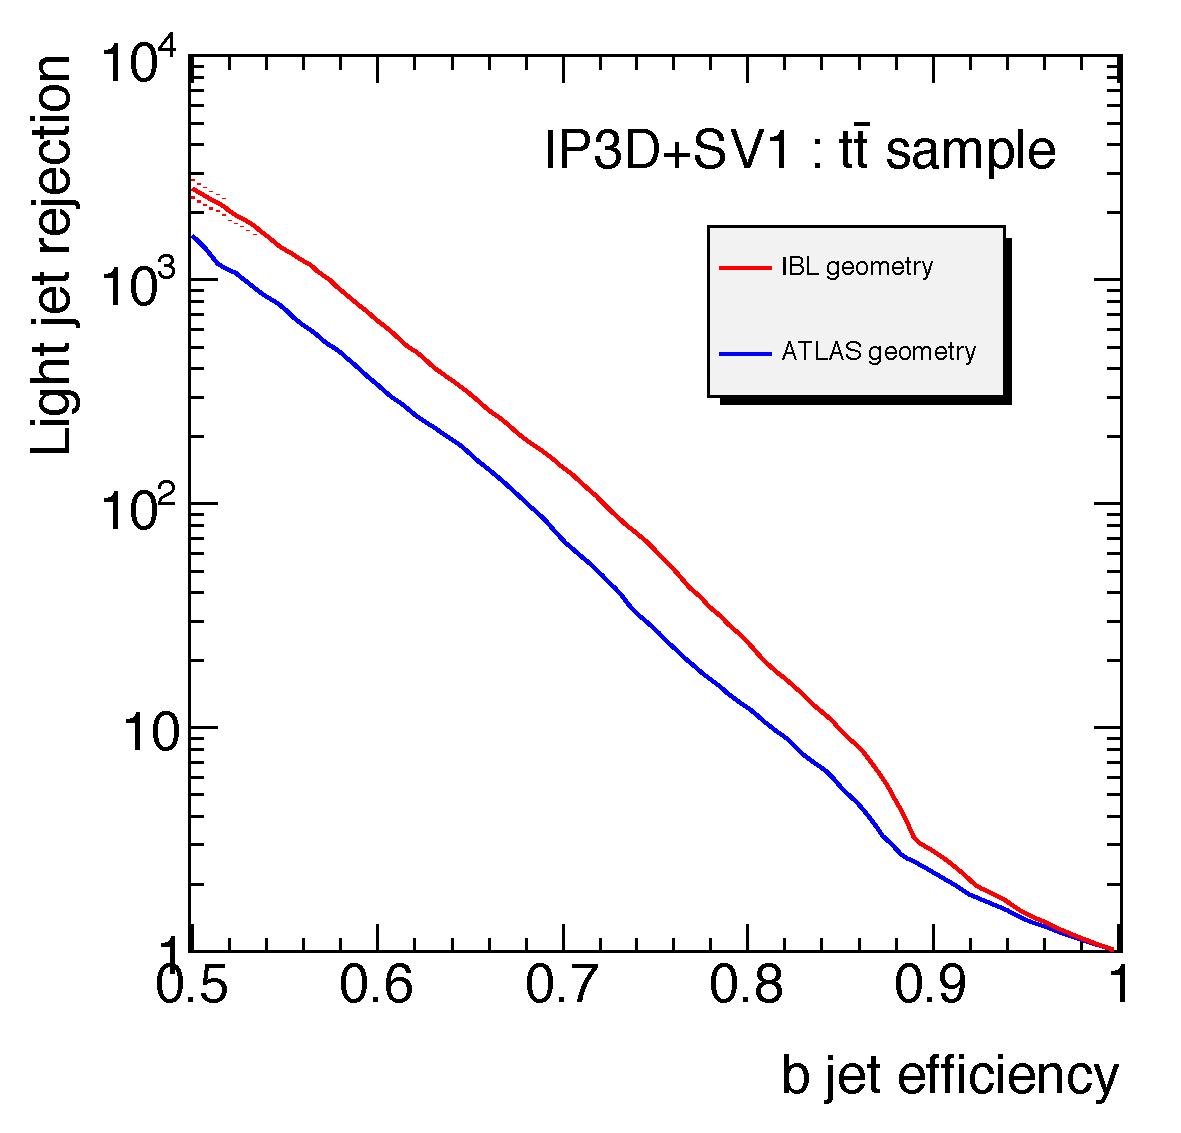
\includegraphics[height=0.44\textwidth]{./figs/IBL_lightrej_factor.pdf}
  \label{sfig:lightrejectionIBL}
}
\caption[Performance of the upgraded pixel detector]{
%
\Fig~\subref{sfig:muontrack} shows one of the first cosmic muon events leaving a track in all four layers of both the new pixel detector including \gls{IBL} and the \gls{SCT}~\cite{ATLASRun2EventDisplays}. 
%
\Fig~\subref{sfig:lightrejectionIBL} shows the \ljet\ rejection factor as a function of the \btag\ efficiency evaluated for the \btag\ algorithm IP3D+SV1 on a \ttbar\ \gls{MC} sample for \gls{ATLAS} with and without the \gls{IBL}~\cite{IBL-TDR}. 
}
\label{fig:IBLsuccess}
\end{figure*}
%%%%%%%%%%%%%%%%%%%%%%%%%%%%%%%%%%%%%%%%%%%%%%%%%%%%%%%%%%%%%%%%%%%%%%%%%%%%%%%







\section{Summary}
\gls{LS1} has been used to prepare the \gls{ATLAS} \gls{ID} for the challenges of \RunTwo. The previous pixel detector has been refurbished and an additional innermost layer of pixel modules, \gls{IBL}, has been inserted. The pixel detector is now in excellent condition and is expected to continue reliable operation throughout \RunTwo, until it will eventually be fully replaced for the conditions of \gls{HLLHC} in 2024.
%
The pixel detector is operating successfully and the new \gls{IBL} detector contributes to the excellent \btag\ performance during \RunTwo. %done

%%%%%%%%%%%%%%%%%%%%%%%% Top quark mass measurements
\chapter{Measurement of the top quark mass at \texorpdfstring{$\sqrts=7$}{sqrt(s)=7}~\TeV}
\label{chap:topmass7TeV}
%
While the data recorded in 2010 allowed for developing physics analyses within the \gls{SM}, the year 2011 marked the beginning of the \gls{LHC} precision measurement era in many fields of particle physics. 
%
Together with the large amount of data provided by the \gls{LHC}, the ever increasing knowledge of the detector and precise theoretical models contributed to a series of successful precision measurements at \gls{ATLAS}. 
%
One of these is the measurement of the \tquark mass in the \dil\ and \ljets\ channels, which has been published early 2015~\cite{Aad:2015nba}. 
%


This chapter presents the analysis in the \dileptonic\ \ttbar\ decay channel with data collected in 2011 at a \cme\ of $\sqrts=7$~\TeV\ at \gls{ATLAS} and is organised as follows:  
%
after the definition of the physical observables, the data and \gls{MC} samples used in the analysis are specified. 
%
The event selection and reconstruction are discussed, based on the definition of physical observables. 
%
The template method is introduced as the way of choice for the determination of the unknown data-inherent parameter, the \tquark mass. 
%
Finally, systematic uncertainty sources are identified, followed by an analysis of their impact on the measurement. 

Unless stated differently, all subsequent analyses are performed using \Root~5.34.12~\cite{Brun199781}, a collection of \Cpp\ libraries for statistical data analysis.






\section{Physics object definition}
\label{sect:physobj7TeV}
As introduced in \sect~\ref{sect:TopQuarkPhysics}, the detector objects resulting from the \tquark pair decay are electron and muon candidates, jets and \met. 
%
They are defined in the following and further reference to any of these reconstructed objects corresponds to the definitions given here. Details to the identification of jet flavours are given as well.
%
More detailed information is given in \reference~\cite{Acharya:1472525}.
%
Throughout this work, the term lepton is used for charged leptons exclusively, whereas non-charged leptons are denoted as neutrinos.

%
\paragraph{Leptons:}\mbox{}
Electron candidates consist of an energy cluster in the \gls{ECAL} and a corresponding well-reconstructed \gls{ID} track~\cite{CERN-PH-EP-2014-040}. 
%
They are required to have a transverse energy of $\et>25$~\GeV, a pseudorapidity of the corresponding \gls{EM} cluster of $\absetaclus < 2.47$, with the transition region $1.37<\absetaclus<1.52$ between the barrel and the end-cap calorimeter excluded. 
%
The reconstruction of muon candidates starts with track segments in the outermost layers of the \gls{MS}~\cite{CERN-PH-EP-2014-151}, consecutively including layers farther inside. 
%
Taking into account effects of the detector material, these segments are then matched to tracks in the \gls{ID}. 
%
After a final fit including the complete track information, the muon candidates are required to satisfy $\pt>20$~\GeV\ and $\vert\eta\vert<2.5$.


The identification of prompt leptons suffers from contamination by heavy-flavour decays inside jets and leptons from photon conversion, referred to as \gls{NP} leptons. 
%
Also, hadrons can mimic lepton signatures and can be misreconstructed as leptons. This is referred to as fake lepton background.
%
To minimise these background contributions, strict isolation criteria are applied to the amount of \gls{EM} activity in the vicinity of the lepton candidate. For the data recorded in 2011, this is defined via a fixed cone size approach.
%
Energy not associated with the lepton cluster within a cone of $\dR = 0.2$ around the candidate is required to be below an $\eta$-dependent threshold, ranging from $1.25$ to $3.7$~\GeV\ for an electron, and $4$~\GeV\ for a muon candidate. These requirements are applied after the subtraction of energy deposits attributed to pile-up, which are typically of the order of $0.5~\GeV$.
%
The total transverse momentum in a cone of $\dR = 0.3$ is similarly restricted and must not exceed a \pt\ and $\eta$ dependent threshold, ranging from $1$ to $1.35$~\GeV, for an electron candidate and a constant threshold of $2.5$~\GeV\ for a muon candidate. 
%
To further reduce the contribution of leptons not stemming from the hard interaction, the longitudinal impact parameter of each charged lepton with respect to the reconstructed primary vertex, defined  as the vertex with the highest $\sum_{\rm trk} p_{\rm T,trk}^2$, among all candidates with at least five associated tracks with $p_{\rm T,trk} > 0.4~\GeV$, is required to be less than 2~\mm.



%
\paragraph{Jets:}\mbox{}
Jets are built from energy clusters in adjacent calorimeter cells, referred to as topological clusters~\cite{Lampl:1099735}, with the \antikt\ jet clustering algorithm~\cite{CAC-0801}, using a radius parameter of $R=0.4$. 
%
A first calibration to the energy scale established for \gls{EM} objects, referred to as \gls{EM} scale, is performed. 
%
Jets are then corrected for in-time and out-of-time pile-up via a pile-up subtraction procedure. 
%
Subsequently, the jet direction is corrected to point to the primary vertex, a procedure referred to as origin correction. After that, jet energy and $\eta$ dependent corrections obtained from simulation are used to calibrate the \gls{EM} jet to the hadronic energy scale. 
%
The final jet energies are obtained with a residual in-situ calibration derived from data and \gls{MC}, calibrating the jet \pt\ against well-reconstructed objects in \Zj\ and \Gammaj\ events~\cite{ATLASCollaboration2015b}. This is the calibration to the \gls{JES}.
%
The entire calibration scheme is referred to as \gls{EM}+\gls{JES} calibration.
%
The jet candidates are required to satisfy $\pt>25$~\GeV.
%
Jets originating from energy deposits not stemming from the hard scattering event, like collisions with residual gas in the beam pipe or calorimeter noise, are identified and rejected by jet quality criteria~\cite{ATLAS-CONF-2012-20}, making use of variables like pulse shape and negative energy measurements in adjacent calorimeter cells.
The amount of low-\pt\ jets originating from pile-up interactions is reduced by requiring associated tracks from the primary vertex to account for at least 75\% of the scalar sum of the \pt\ of all tracks within the jet. This quantity is referred to as \gls{JVF}. Jets with no associated tracks are also accepted. In the data recorded in 2011, this requirement is applied to all jets, regardless of their kinematic properties.
%
The contamination by muons from hadron decays within jets is reduced by removing muons from the event, which are reconstructed within a $\dR=0.4$ cone around the axis of a jet and satisfy $\pt>25$~\GeV. 
%
Electron clusters are usually also reconstructed as jets and, therefore, jets within a $\dR=0.2$ cone around an electron candidate are removed to avoid double-counting. 
%
Finally, electrons are rejected if their spatial distance to the closest jet is smaller than $\dR=0.4$.


%
\paragraph{\boldmath$\met$:}\mbox{}
The construction of the \met\ is based on the vector sum of energy deposits in the calorimeters, projected onto the transverse plane. 
%
Calorimeter clusters are treated at the \gls{EM} scale and subsequently corrected according to the energy scale of the corresponding identified physics object. Muons are included using their momentum, reconstructed in the \gls{ID} and \gls{MS}~\cite{ATLAS-MET-NEW}. 



%
\paragraph{Flavour tagging:}\mbox{}
The identification of the underlying jet flavour is of high importance for the reconstruction of \tquark\ pair events and is referred to as flavour tagging. 
%
Most important for the \ttbar\ decay reconstruction is the process of identifying a jet originating from a \bquark, the \btag. 
%
In the following, irrespective of their origin, jets tagged by the algorithm are referred to as \btagged\ jets, whereas those not tagged are referred to as untagged jets. 
%
Similarly, whether they are tagged or not, jets originating from \bquark{s}\ are referred to as \bjet{s}\ and those from $u, d, c, s$-quarks or gluons as \ljet{s}.
%
The \bhadron\ properties like invariant mass, long lifetime and large branching fraction of the decay to leptons can be used for discrimination. A direct consequence of the long lifetime of the \bhadron\ is the significant decay length, resulting in a large distance of the decay vertex from the primary vertex and large jet track impact parameters. This information is input to \btag\ algorithms, which determine a \btag\ discrimination weight, corresponding to a probability for a given jet to originate from a \bquark. 
%
The strategy adopted here relies on the neural network-based MV1 algorithm~\cite{Aad:2015ydr}. It combines the weights of the \btag\ algorithms JetFitter, IP3D and SV1~\cite{Aad:2015ydr} with information on the jet \pt\ and $\eta$ to form a discriminant variable $w$, using a neural network in a \gls{MVA}. Light quark and gluon jets populate the lower regions of the $w$ phase space, \cflavoured\ jets adopt values of $w\approx0.5$ and \bflavoured\ jets have values close to $w=1$. A cut-off, referred to as working point and chosen according to the needs of the analysis, is applied to the discriminating variable. It determines the algorithm efficiency, i.e. the probability for a \bjet\ to be \btagged, and the rejection factor, i.e. the number of untagged \ljet{s} per one mistagged \ljet. 
%
The MV1 working point for this analysis is chosen to correspond to an average \btag\ efficiency of 75\% for \bjet{s}\ in simulated \ttbar\ events and a \ljet\ (\cjet) rejection factor of 64 (4). 
%This efficiency is highly \pt\ dependent.
%$w=0.404219$
To match the \btag\ performance in the data, \pt-dependent scale factors, obtained from dijet and \ttbarll~\cite{Aad:2015ydr} events, are applied to MC jets depending on their true flavour. 
%
The \btag\ efficiency is determined from \ttbarll\ events. A combinatorial likelihood is formed using \ljet\ efficiencies and \bquark\ multiplicities from simulation and \btagged\ jet multiplicities measured in data. The likelihood considers the correlations of jets in the same event, thus outperforming previous equation-based determinations~\cite{Aad:2015ydr}. The scale factors are defined as the \btag\ efficiency ratio of \bjet{s} in data and \gls{MC}. A significant jet $\eta$-dependence is not observed.
%
The per jet scale factors are multiplied to obtain the \gls{MC} event weight.
























\section{Data and Monte Carlo samples}
\label{sect:dataMC7TeV}
%
The \tquark\ mass measurement presented in this chapter is based on \gls{LHC} data, recorded by the \gls{ATLAS} experiment in the year 2011 with a \pp\ \cme\ of $\sqrts=7$~\TeV. 
%
The triggers used are single-electron or single-muon triggers, operating with an electron threshold of 20 or 22~\GeV, depending on the data-taking period, and a muon threshold of 18~\GeV. Recorded events therefore stem from the electron-photon (\Egam) and the \Muon\ data stream. Double-counting is avoided by only accepting a \Muon\ triggered event if it was not present in the \Egam\ stream. 
%
The integrated luminosity, recorded with stable beam conditions and all relevant detector components operational, amounts to $\intlumi=4.6~\invfb$ with an uncertainty of 1.8\%~\cite{Aad:2013ucp}. 


The modelling of \ttbar, single \tquark\ and most background processes relies on \gls{MC} simulations. 
%
For \tquark\ pair and single \tquark\ production in the s- and $Wt$-channel, the \gls{NLO} program \Powheg-hvq (patch4)~\cite{FRI-0701} with the NLO CT10~\cite{LAI-1001} \gls{PDF} and the parameter $\hdamp=\infty$, controlling the matrix element to \gls{PS} matching, is used.
%
The \Acermc\ (v3.8) generator~\cite{SAMPLES-ACER} interfaced with \Pythia (v6.425) provides the simulation of the single top quark t-channel process. 
%
The \Acermc\ and \Pythia\ programs are used with the CTEQ6L1 \glspl{PDF} and the corresponding Perugia 2011C (P2011C) parameter set~(tune)~\cite{Skands}.
%
The \Pythia\ (v6.425)~\cite{SJO-0601} program with the P2011C tune and the corresponding CTEQ6L1 \glspl{PDF}~\cite{Pumplin2002} are employed to model processes, which are not attributed to the hard scattering, like the \gls{PS}, the hadronisation and the underlying event. 
%
For \mt\ hypothesis testing, the \ttbar\ and single top quark production samples are generated for different assumed values of \mt\ in the range $167.5$ to $177.5$~\GeV\ in steps of $2.5$~\GeV.
%
For each \mt\ value, the \ttbar\ MC samples are normalised to the predicted \ttbar\ cross section for \pp\ collisions at $\sqrts = 7$~\TeV, which was calculated at \gls{NNLO} in \gls{QCD} including resummation of \gls{NNLL} soft gluon terms with Top++~2.0~\cite{CAC-1101,PRL-109-132001,JHEP-1212,JHEP-1301,Czakon:2013goa,CZA-1101}.
%
% The \ttbar\ cross section is $\sigma_{\ttbar}= 177^{+10}_{-11}$~\pb\ for $\mt=172.5$~\GeV.
%
% The \gls{PDF}+\alphas\ uncertainties on the cross section were calculated using the PDF4LHC prescription~\cite{PDF4LHC} with the MSTW2008 $68\%$ CL~NNLO~\cite{MAR-0901,MAR-0902}, CT10~NNLO~\cite{LAI-1001,CT10NNLO} and NNPDF2.3~5f~FFN~\cite{Ball:2012cx} \glspl{PDF}, and added in quadrature to the factorisation and renormalisation scale uncertainty. 
%
% The \gls{NNLO}+\gls{NNLL} value, as implemented in Hathor~1.5~\cite{ALI-1101}, is about $3\%$ larger than the plain \gls{NNLO} prediction. %too detailed

The single \tquark\ production cross sections are normalised to the approximate \gls{NNLO} prediction values. 
%
At $\mt=172.5$~\GeV, these are $64.6^{+2.7}_{-2.0}$~\pb~\cite{Kidonakis:2011wy}, $15.7\pm 1.1$~\pb~\cite{Kidonakis:2010ux} and $4.6\pm 0.2$~\pb~\cite{Kidonakis:2010tc} for the t-, $Wt$- and the s-channels, respectively. 
%
% The corresponding \gls{LO} Feynman diagrams are shown in \fig{s}~\subref*{sfig:tchanfeyn},\subref{sfig:Wtchanfeyn} and \subref{sfig:schanfeyn}, respectively.  
%
The \Alpgen (v2.13) generator~\cite{MAN-0301} interfaced to the \Herwig\ (v6.520)~\cite{COR-0001} and \Jimmy\ (v4.31)~\cite{SAMPLES-JIMMY} packages is used for the simulation of \Wbos\ or \Zboson{s} in association with jets. 
%
The CTEQ6L1 \glspl{PDF} and the corresponding AUET2 tune~\cite{ATL-PHYS-PUB-2011-008} are used for the matrix element and \gls{PS} settings. 
%
The \Wj\ events containing heavy-flavour quarks ($Wbb$+jets, $Wcc$+jets, and $Wc$+jets) are generated separately with \gls{LO} matrix elements involving massive bottom and \cquark{s}. 
%
Double-counting of heavy-flavour quarks in the matrix element and the \gls{PS} evolution is avoided via a \gls{HFOR} procedure~\cite{TwikiHFOR}. 
%
Diboson production processes ($WW$, $WZ$ and $ZZ$) are produced using the \Herwig\ generator with the AUET2 tune.



\Pythia (v6.425) with the AMBT2B tune~\cite{ATL-PHYS-PUB-2011-009} is used to generate multiple soft \pp\ interactions. 
%
After being added to all \gls{MC} samples, these simulated events are reweighted until the distributions of the pile-up related quantities \meanmu\ and \nvtx\ in the simulated samples match the ones observed in the data. 
%
These are $\meanmu=8.8$ and $\langle\nvtx\rangle=7.0$ for the dataset considered. These values are analysis-specific due to the event selection.
 % and do not necessarily match the values in \fig~\ref{sfig:meanmu}.
%
Finally, the samples undergo a simulation of the ATLAS detector~\cite{WT-ATLAS-SIMULATION-PAPER} based on \Geantfour~\cite{AGO-0301} and are from then on processed through the same reconstruction software as the data. Due to limited computing resources, many samples used to assess systematic uncertainties, have been produced bypassing the highly computing intensive full \Geantfour\ simulation with the fast simulation package \Atlfast~\cite{Richter-Was:683751}. It uses smearing functions and interpolates particle behaviour and detector response, based on resolution functions measured in full simulation studies, to approximate the results of the full simulation of the calorimeters, where particle interactions are most complex. 









\section{Event selection and reconstruction}
\label{sect:evselreco7TeV}
%
The \ttbarll\ channel is characterised by the presence of two high-\pt\ leptons with opposite charge, large \met\ originating from the two invisible neutrinos, and two \bjet{s}. 
%
This final state is similar to the ones of a number of other processes. The dominant contribution of this physics background arises from the single \tquark\ production in the $Wt$ channel. With leptonically decaying \Wboson{s}, this process contains two leptons, \met\ and potentially two or more jets in the final state. If one of those is mistagged as \bjet, the process mimics the \dil\ final state. 
%
Leptonic \Zboson\ decays accompanied by two or more jets and diboson processes provide additional sources of background. 
%
These processes are estimated from \gls{MC}, normalised to their respective cross sections. 
%

The contribution of events wrongly reconstructed as \ttbarll\ events due to the presence of \fake{s} is estimated from data. 
%
The technique employed here uses fake and real lepton efficiencies measured in a background enhanced control region with low \met\ and a region around the \Zboson\ peak, where true leptons can easily be identified. 
%
From this, fake lepton efficiencies as a function of the lepton $\eta$ and $p_T$ are derived.
%
Using two sets of lepton identification quality requirements, a loose and a tight definition, in a matrix method~\cite{Aad:2010ey}, a fake lepton weight is assigned to each event in the data, representing the probability of containing a \fake. 
%
The expected \fake\ yield is extracted from the data sample, rescaled by these weights.
%
This procedure also accounts for the contribution of \Wj\ events to the background, which only involves a single prompt lepton.










\subsection{Event selection}
\label{sect:evsel7TeV}
To select the relevant processes from the vast amount of data, an analysis-specific series of selection criteria is applied to general event quality variables and reconstructed objects. 
%
These criteria have been established to select a maximum amount of signal events while minimising the pollution from background. 
%
They are either positively formulated, such as requiring the presence of a certain physical object, or negatively by vetoing it:
%
\begin{enumerate}
\item Events are required to have at least one good primary vertex. 
%
This suppresses non-collision background events.
\item A signal from the corresponding single-electron or single-muon trigger is required.
\item Exactly two oppositely charged leptons are required, with at least one of them matching the trigger object.
\item In the same lepton flavour channels, \ee\ and \mumu, $\met>60~\GeV$ is required. This reduces background contributions like the one from \Zj\ events.
\item In the \emu\ channel, $\Ht>130~\GeV$ is required, with \Ht\ being the scalar sum of \pt\ of the two selected leptons and all jets. This requirement reduces the background from \Zj\ and diboson events.
\item In the same lepton flavour channels, the invariant mass of the lepton pair is required to satisfy $m_{\ell\ell} > 15~\GeV$. 
%
This reduces Drell--Yan production and low-mass resonance backgrounds decaying into charged lepton--anti-lepton pairs.
\item  To reduce background from \Zboson\ production, in the same lepton flavour channels events with lepton--lepton system invariant mass values $m_{\ell\ell}$ compatible within $10$~\GeV\ with the \Zboson\ mass are excluded.
\item The presence of least two jets with $\pt>25$~\GeV\ and $\vert\eta\vert<2.5$ is required.
\item Exactly one or two of these jets have to be \btagged.
\end{enumerate}

An overall count of 6661 data events satisfies these requirements. 
















\subsection{Event reconstruction}
\label{sect:dilreco7TeV}
After the selection of events, the different objects therein are related to the corresponding \gls{LO} decay hypothesis via an event reconstruction. 
%
Since the electric charge of quarks cannot be measured with sufficient accuracy from the observed jet, the matching of reconstructed jets and their ancestor partons at \genlevel is ambiguous and has to be assessed using channel-specific techniques.



In the \ttbarll\ channel, the two neutrinos in the final state mostly account for the observed \met. 
%
Consequently, the system of kinematic equations is underconstrained and a full reconstruction of the event decay kinematics is not possible without additional assumptions. 
%
Two approaches to overcome this limitation are in use: the reconstruction of the most probable full decay configuration and the reconstruction of subsystems of the decay.
%
The full reconstruction techniques rest on estimations of the most probable neutrino four-momenta, given the event-specific decay kinematics~\cite{PhysRevD.92.032003,CMS-PAS-TOP-14-010,D0:2015dxa}.
%
These techniques exploit \gls{MC} based hypotheses for neutrino momenta, pseudorapidity $\eta$ or azimuthal angle $\phi$ distributions to construct a per-event likelihood and use the most probable solution to reconstruct \mt. 
%
However, these approaches do not yield a significant advantage in terms of systematic uncertainties~\cite{Maier2012} and are often outperformed by partial reconstruction approaches, like the one pursued in this work. 
%
Instead of using the maximum amount of information available, it uses the least necessary, while keeping a high sensitivity to \mt. 
%
A full event reconstruction is not performed and also the use of the \met variable is avoided, since despite the information on the event kinematics, the uncertainties connected with it deteriorate the final precision. This has been shown for two estimators, closely connected but for their usage of \met. 
%
Furthermore, the partial reconstruction has been shown to be superior in terms of total uncertainty~\cite{Maier2012}.
%
The  \mlb\ estimator yields the best final precision on \mt\ among those investigated and is used in this analysis. 



%dilepton reco
The \mlb\ estimator is defined as the average invariant mass of the two lepton--\bjet\ pairs, $\mlb=(\mlbplus+\mlbminus)/2$. 
%
In the case of exactly two \btagged\ jets, there are two possible assignments for the jet--lepton pairs, each leading to a different value of \mlb. 
%
The combination leading to the lowest \mlb\ value is retained and the \bjet{s} are assigned to the \tquark\ or anti-\tquark, according to the lepton charge. 
%
In the case of only one \btagged\ jet, the jet carrying the next highest MV1 \btag\ weight is taken as second \bjet. 
%
This also allows for the single \tquark\ contributions to be treated as signal and to exploit their inherent sensitivity to \mt.
%
Finally, the measured \mlbr\ is required to be in the range 30~\GeV\ to 170~\GeV. 
%
This extra selection retains 97\% of the candidate events in data. 
%
With a total of 6476 data events, the expected background fraction is 2\%. 











\subsection{Event yields}
\label{sect:evtyields7TeV}
The observed and expected numbers of events at an input \tquark\ mass of $\mt=172.5$~\GeV\ after the above selection are reported in \tab~\ref{tab:stdselDL7TeV}. 
%
For both \btag\ multiplicities, the observed numbers of events are in agreement with the sum of the signal and background estimates within uncertainties. 
%
The quoted uncertainties are the sum in quadrature of the statistical uncertainty, the uncertainty on the \btag\ efficiency, a 1.8\% uncertainty on the integrated luminosity~\cite{Aad:2013ucp}, the uncertainties on the \ttbar\ and single \tquark\ theoretical cross sections, a 30\% uncertainty on the \Wj\ and \Zj\ normalisation and finally a 50\% uncertainty on the \fake\ background normalisation.
% 
The distributions of several kinematic variables in the data were inspected and found to be well described by the prediction.
%
As examples, \fig~\ref{fig:DLdataMCcomp7TeV} shows jet multiplicities and the \pt\ and $\eta$ distributions for the leptons and \btagged\ jets. \Fig~\ref{fig:DLdataMCcomp7TeV2} shows the \met, the \mlbr\ and the \pt\ distributions of the dijet and \dil\ systems. 
%
The \gls{MC} prediction assumes an input \tquark\ mass of 172.5~\GeV. 
%
%%%%%%%%%%%%%%%%%%%%%%%%%%%%%%%%%%%%%%%%%%%%%%%%%%%%%%%%%%%%%%%%%%%%%%%%%%%%%%%
\begin{table}[tbp!]
\begin{center}
\small
\begin{tabular}{|l|rr|rr|rr|}
\hline
Process             & \multicolumn{2}{c|}{$=1$ \btagged\ jet} 
										& \multicolumn{2}{c|}{$=2$ \btagged\ jets} 
										& \multicolumn{2}{c|}{Sum} \\
\hline
\ttbar\   signal         &  2840 $\pm$ &   180  & 2950  $\pm$ &  210 &  5790 $\pm$ &   360\\
Single \tquark\ (signal) &   181 $\pm$ &    10  & 82.5  $\pm$ &  5.7 &   264 $\pm$ &    15\\
\fake{s}            &    52 $\pm$ &    28  &  2.6  $\pm$ &  8.4 &    55 $\pm$ &    30\\
\Zj\                &    34 $\pm$ &    11  &  4.1  $\pm$ &  1.5 &    38 $\pm$ &    12\\
$WW/WZ/ZZ$          &  7.01 $\pm$ &  0.63  & 0.61  $\pm$ & 0.15 &  7.62 $\pm$ &  0.67\\\hline
Signal+background   &  3110 $\pm$ &   180  & 3040  $\pm$ &  210 &  6150 $\pm$ &   360\\\hline
Data                & \multicolumn{2}{c|}{3227} 
                    & \multicolumn{2}{c|}{3249} 
                    & \multicolumn{2}{c|}{6476} \\\hline
Exp. bkg. frac.     & 0.03 $\pm$ & 0.00 & 0.00 $\pm$ & 0.00 & 0.02 $\pm$ & 0.00 \\
Data/MC             & 1.04 $\pm$ & 0.06 & 1.07 $\pm$ & 0.07 & 1.05 $\pm$ & 0.06 \\\hline
\end{tabular}
\end{center}
\caption[Event yields for $\sqrts=7$~\TeV\ data]{
%
The observed numbers of events in $\intlumi=4.6$~\invfb\ of $\sqrts = 7$~\TeV\ data, divided into \btagged\ jet multiplicity. 
%
In addition, the expected numbers of signal and background events corresponding to the integrated luminosity of the data are given. 
%
Two significant digits are used for the uncertainties of the predictions.
% 
Values smaller than $0.005$ are listed as $0.00$.
%
}
\label{tab:stdselDL7TeV}
\end{table}
%%%%%%%%%%%%%%%%%%%%%%%%%%%%%%%%%%%%%%%%%%%%%%%%%%%%%%%%%%%%%%%%%%%%%%%%%%%%%%%
%
%%%%%%%%%%%%%%%%%%%%%%%%%%%%%%%%%%%%%%%%%%%%%%%%%%%%%%%%%%%%%%%%%%%%%%%%%%%%%%%
\begin{figure*}[tbp!]
\centering
\subfloat[Number of jets]{
  \includegraphics[width=0.49\textwidth]{./figs/Plot_3dTMT_dataMC_finalnjet_s1725_seltype5.pdf}
  \label{sfig:llnjets}
}
\subfloat[Number of \btagged\ jets]{
  \includegraphics[width=0.49\textwidth]{./figs/Plot_3dTMT_dataMC_finalntag_s1725_seltype5.pdf}
  \label{sfig:llntaggedjets}
}
\hfill
\subfloat[\btagged\ jets \pt]{
  \includegraphics[width=0.49\textwidth]{./figs/Plot_3dTMT_dataMC_BjetPt_s1725_seltype5.pdf}
  \label{sfig:lltaggedjetspt}
}
\subfloat[Lepton \pt]{
  \includegraphics[width=0.49\textwidth]{./figs/Plot_3dTMT_dataMC_LepPt_s1725_seltype5.pdf}
  \label{sfig:llleptonspt}
}
\hfill
\subfloat[\btagged\ jets  $\eta$]{
  \includegraphics[width=0.49\textwidth]{./figs/Plot_3dTMT_dataMC_BjetEta_s1725_seltype5.pdf}
  \label{sfig:lltaggedjetseta}
}
\subfloat[Lepton $\eta$]{
  \includegraphics[width=0.49\textwidth]{./figs/Plot_3dTMT_dataMC_LepEta_s1725_seltype5.pdf}
  \label{sfig:lltaggedleptonseta}
}
\hfill
\caption[Data to \gls{MC} comparison for $\sqrts=7$~\TeV\ data: direct observables]{
\Fig{s}~\subref{sfig:llnjets} and \subref{sfig:llntaggedjets} show the jet and \btagged\ jet multiplicity, \fig{s}~(c, d) and (e, f) show the distributions of the lepton and \btagged\ jets \pt\ and $\eta$. 
%
The data are shown by the points with statistical uncertainty bars, and the predictions are shown by the solid histograms. 
%
The hatched area is the combined uncertainty on the prediction described in \sect~\ref{sect:evtyields7TeV}, and the rightmost bin contains the overflow, if present. 
%
For each figure, the ratio of the data to the \gls{MC} prediction is also presented.
%
  \label{fig:DLdataMCcomp7TeV}}
\end{figure*}
%%%%%%%%%%%%%%%%%%%%%%%%%%%%%%%%%%%%%%%%%%%%%%%%%%%%%%%%%%%%%%%%%%%%%%%%%%%%%%%
%
%%%%%%%%%%%%%%%%%%%%%%%%%%%%%%%%%%%%%%%%%%%%%%%%%%%%%%%%%%%%%%%%%%%%%%%%%%%%%%%
\begin{figure*}[tbp!]
\centering
\subfloat[\met]{
  \includegraphics[width=0.49\textwidth]{./figs/Plot_3dTMT_dataMC_Met_s1725_seltype5.pdf}
  \label{sfig:llmet}
}
\subfloat[\mlbr]{
  \includegraphics[width=0.49\textwidth]{./figs/Plot_3dTMT_dataMC_mlb_s1725_seltype5.pdf}
  \label{sfig:llmlb}
}
\hfill
\subfloat[\ptbb]{
  \includegraphics[width=0.49\textwidth]{./figs/Plot_3dTMT_dataMC_pTbb_s1725_seltype5.pdf}
  \label{sfig:llptbb}
}
\subfloat[\ptll]{
  \includegraphics[width=0.49\textwidth]{./figs/Plot_3dTMT_dataMC_pTll_s1725_seltype5.pdf}
  \label{sfig:llptll}
}
\hfill
\caption[Data to \gls{MC} comparison for $\sqrts=7$~\TeV\ data: derived observables]{
%
Same as \fig~\ref{fig:DLdataMCcomp7TeV} but \fig{s}~\subref{sfig:llmet} and \subref{sfig:llmlb} show the \met\ and \mlbr\ distributions. \Fig{s}~\subref{sfig:llptbb} and \subref{sfig:llptll} show the \pt\ distributions of the dijet and \dil\ systems.
%
  \label{fig:DLdataMCcomp7TeV2}}
\end{figure*}
%%%%%%%%%%%%%%%%%%%%%%%%%%%%%%%%%%%%%%%%%%%%%%%%%%%%%%%%%%%%%%%%%%%%%%%%%%%%%%%


































\clearpage






\section{The template method}
The analysis method employed in this work is the template method. 
%
Templates are simulated distributions of an estimator, constructed for a number of discrete values of the parameter under study, in this case for different \mt values. 
%
Appropriate functions are then fitted to these templates, interpolating between different input values of the physics parameter. 
%
The remaining parameters of the functions are fixed by a simultaneous fit to all templates, imposing linear dependences of the parameters on \mt. 
%
The resulting template fit function has \mt as the only free parameter and an unbinned likelihood maximisation yields the value of \mt\ that best describes the data. 
%
This procedure is detailed in the following.












\subsection{Construction of the likelihood function}
\label{sect:like7TeV}

The signal templates are distributions of \mlbr, based on independent \gls{MC} samples, using different input values of \mt in the range of $167.5$ to $177.5$~\GeV\ in steps of $2.5$~\GeV.
%
The \mlbr\ estimator distribution and its dependency on the underlying \gls{MC} \mt\ value are shown in \fig~\ref{fig:templtop7TeV} for events with exactly two \btagged\ jets. 
%
%%%%%%%%%%%%%%%%%%%%%%%%%%%%%%%%%%%%%%%%%%%%%%%%%%%%%%%%%%%%%%%%%%%%%%%%%%%%%%%
\begin{figure*}[tbp!]
\centering
% \subfloat[\mlbr\ for exactly two \btagged\ jets]{
	\includegraphics[width=0.6\textwidth]{./figs/MC_fit_wp75_mlb_overlaid_ele0_dep0.pdf}
	% \label{sfig:mlbrmtop}
% }
\caption[Template fit functions for $\sqrts=7$~\TeV\ data]{
%
The distribution of \mlbr\ for different values of the input \mt\ for \gls{MC} signal events with exactly two \btagged\ jets. 
%
The corresponding \glspl{pdf} are displayed on top of the distributions.
%
\label{fig:templtop7TeV}}
\end{figure*}
%%%%%%%%%%%%%%%%%%%%%%%%%%%%%%%%%%%%%%%%%%%%%%%%%%%%%%%%%%%%%%%%%%%%%%%%%%%%%
%
%
The sum of a Gaussian and a Landau function is fitted to the \mlbr\ signal templates produced with different \mt\ values. 
%
A Landau function is fitted to the background template. 
%
Since the single \tquark\ contribution with its \tquark\ mass dependence is included in the signal, the background templates are insensitive to and not parametrised as a function of \mt. 
%
The fits are done separately for events with exactly one or exactly two \btagged\ jets. 
%
After verifying that all fit parameters of the separate fits depend linearly on \mt, the linearity is imposed and used to fix all other parameters in a combined fit to all templates. An example for this procedure can be found in \reference~\cite{Maier2012}.
%
The resulting signal and background \glspl{pdf} are used in an unbinned likelihood fit to the data.
%
The likelihood function, maximised for $N$ data events, is
%
%%%%%%%%%%%%%%%%%%%%%%%%%%%%%%%%%%%%%%%%%%%%%%%%%%%%%%%%%%%%%%%%%%%%%%%%%%%%%%%
\[
\Like(\mt, \fbkg) = 
\prod_{i=1}^{N} 
\left[ (1-\fbkg)\cdot \Ptopsig(\mlbri \,\vert\, \mt) + \fbkg \cdot \Ptopbkg(\mlbri) \right],
\]
%%%%%%%%%%%%%%%%%%%%%%%%%%%%%%%%%%%%%%%%%%%%%%%%%%%%%%%%%%%%%%%%%%%%%%%%%%%%%%%
%
with \Ptopsig\ and \Ptopbkg\ denoting the signal and background \glspl{pdf} and \fbkg\ the fraction of background events in the selected data sample.

% %
%%%%%%%%%%%%%%%%%%%%%%%%%%%%%%%%%%%%%%%%%%%%%%%%%%%%%%%%%%%%%%%%%%%%%%%%%%%%%%%%%%%%%%
\begin{figure*}[tbp!]
\centering
\subfloat[\mt\ residual]{
  % \includegraphics[width=0.49\textwidth,trim={460 210 0 0},clip]{./figs/Plot_Pexp_RlbCalo_dim0_shape_2_ele2_bkgfr_002wc_501_pe_4600_invpb_summary.pdf}
  \includegraphics[height=0.4\textwidth]{./figs/bias7TeV.png}
  \label{sfig:bias7TeV}
}
\subfloat[Pull width]{
  \includegraphics[height=0.4\textwidth]{./figs/pullwidth7TeV.png}
  \label{sfig:pullwidth7TeV}
}
\caption[\mt\ residuals and pull widths for $\sqrts=7$~\TeV\ data]{
%
\Fig~\subref{sfig:bias7TeV} shows the \mt\ residuals observed when applying the method to the respective input templates and \fig~\subref{sfig:pullwidth7TeV} shows the pull distribution width.
%
The dashed lines correspond to the expected values of zero and one respectively. The full lines are the result of a fit of a constant to the points. 
%
\label{fig:pulls7TeV}
}
\end{figure*}
%%%%%%%%%%%%%%%%%%%%%%%%%%%%%%%%%%%%%%%%%%%%%%%%%%%%%%%%%%%%%%%%%%%%%%%%%%%%%%%%%%%%%%
%
The consistency of the method and the expected statistical uncertainty corresponding to the data sample of $\intlumi=4.6$~\invfb\ is examined using pseudo-experiments. 
%
These are performed by randomly drawing events from the signal and background samples and then applying the aforementioned likelihood to this pseudo-dataset to extract its \mt\ value. 
%
These pseudo-experiments are performed 500 times per mass point and corrected for oversampling~\cite{BarlowCF}, following the procedure used in \reference~\cite{Maier2012}. The results are shown in \fig~\ref{fig:pulls7TeV}. No significant deviation is found between the known input parameters \mtin\ and the results of the fits \mtout. This means that the method is unbiased.
%
For all mass points the distribution of the pull $(\mt-\mt^\mathrm{fit})/\sigma^\mathrm{fit}$, the per pseudo-experiment deviation of the fit result from the expected underlying \mt\ value normalised to the uncertainty, exhibits a mean and width value consistent with the expectation of zero and one within the statistical uncertainties. 
%
This means the statistical uncertainties are correctly evaluated. 
%
The expected statistical uncertainties for $\mt=172.5$~\GeV\ in the exactly one or two \btagged\ jets case are determined to be $0.95\pm0.04$~\GeV\ and $0.65\pm0.02$~\GeV, respectively. The values quoted are the means and standard deviations of the distributions of the statistical uncertainties of the fitted masses from the pseudo-experiments. 
%
The different statistical power is not a consequence of different numbers of events, as can be seen from \tab~\ref{tab:stdselDL7TeV}, but of the superior inherent resolution on \mt\ for events with two \btagged\ jets compared to events with only one \btagged\ jet.

The final \mt\ measurement is performed by multiplication of the per event \btagged\ jet multiplicity-specific likelihood. 
%
The \mt\ value is required to be the same for the two \btagged\ jet multiplicity-specific sub-samples. 
%
However, the background fractions are treated as separate parameters in the two sub-samples, corresponding to two individual parameters ($f_\mathrm{bkg}^{1b}$, $f_\mathrm{bkg}^{2b}$). 
%
Analysing the two sub-samples in a combined likelihood fit reduces statistical uncertainties and mitigates some systematic effects. The correlation between the fitted parameters is shown in \tab~\ref{tab:bkgmtopcorr}.
%
For this likelihood fit, the expected statistical precision on the \mt\ measurement for $\mt=172.5$~\GeV\ is $0.54 \pm 0.01$~\GeV. 
%
%%%%%%%%%%%%%%%%%%%%%%%%%%%%%%%%%%%%%%%%%%%%%%%%%%%%%%%%%%%%%%%%%%%%%%%%%%%%%%%
\begin{table*}[tb!]
%\footnotesize
% \small
\begin{center}
\begin{tabular}{|r||rrr|}%\cline{2-6}
\hline
& \mt & $f_{\rm bkg}^{1b}$ & $f_{\rm bkg}^{2b}$ \\ \hline
\mt                     &  1.00 &       &         \\  
 $f_{\rm bkg}^{1b}$  &  0.07 &  1.00 &         \\
 $f_{\rm bkg}^{2b}$  & --0.14 & --0.01&  1.00    \\  \hline
\end{tabular}
\end{center}
\caption[Correlation of the fitted parameters]{
%
The correlations of the fitted parameters used in the likelihood maximisation.
%
\label{tab:bkgmtopcorr}}
\end{table*}
%%%%%%%%%%%%%%%%%%%%%%%%%%%%%%%%%%%%%%%%%%%%%%%%%%%%%%%%%%%%%%%%%%%%%%%%%%%%%
%









\section{Result in the data}
% \label{sec:result}

The likelihood fit to the data yields
%
%%%%%%%%%%%%%%%%%%%%%%%%%%%%%%%%%%%%%%%%%%%%%%%%%%%%%%%%%%%%%%%%%%%%%%%%%%%%%%%
\[
 \mt = \XZst{173.79}{0.54}~\GeV.
\]
%%%%%%%%%%%%%%%%%%%%%%%%%%%%%%%%%%%%%%%%%%%%%%%%%%%%%%%%%%%%%%%%%%%%%%%%%%%%%%%
%
The corresponding fitted values of the background fraction are $3.5\% \pm 3.7\%$ and $1.4\% \pm 2.2\%$ for one \btagged\ jet and the two \btagged\ jets samples. 
%
These fractions are consistent with the expectations given in \tab~\ref{tab:stdselDL7TeV} and also with no background at all. 
%
\Fig~\subref*{sfig:mlbrecofit} shows the \mlbr\ distribution in the data together with the corresponding fitted \glspl{pdf} for the background alone and for the sum of signal and background for the combined one and two \btagged\ jets samples. 
%
The uncertainty band is the envelope of all \glspl{pdf}, obtained from 500 pseudo-experiments with fixed background fractions while varying the fitted \mt\ within $\pm 1\sigma$ of its full uncertainty, including the systematic effects to be discussed below. 
%
Within this band, the data are well described by the fitted \gls{pdf}.
%


The likelihood profile as a function of \mt\ is reported in \fig~\subref*{sfig:llmtoplike} for the sample with one \btagged\ jet, the sample with two \btagged\ jets and the combined \ttbarll\ result.
%
The figure demonstrates the consistency of the measured \mt\ values in the samples with different \btagged\ jet multiplicities.
%
%
%%%%%%%%%%%%%%%%%%%%%%%%%%%%%%%%%%%%%%%%%%%%%%%%%%%%%%%%%%%%%%%%%%%%%%%%%%%%%%%
\begin{figure*}[tbp!]
\centering
\subfloat[Fit to the data]{
	\includegraphics[height=0.37\textwidth]{figs/Fit_data_rlbcalo_mlb_ele2_4600invpb.pdf}
	\label{sfig:mlbrecofit}
}
\subfloat[\mt\ likelihood profile]{
	\includegraphics[height=0.37\textwidth]{figs/Compare_1and2btag_results_3.pdf}
	\label{sfig:llmtoplike}
}
%
\caption[Likelihood fit for $\sqrts=7$~\TeV\ data]{
%
\Fig~\subref{sfig:mlbrecofit} shows the data distribution for one and two \btagged\ jets of \mlbr\ and the fitted \glspl{pdf} for the background alone and for signal-plus-background, using an unbinned likelihood fit. 
%
The uncertainty band indicates the total uncertainty on the signal-plus-background fit obtained from pseudo-experiments as explained in the text. 
%
\Fig~\subref{sfig:llmtoplike} shows the likelihood profile as a function of \mt, denoted by \mtdl\ in the figure, for the sample with one \btagged\ jet (grey), the sample with two \btagged\ jets (red) and the combined result (blue). 
%
\label{fig:results7TeV}}
\end{figure*}
%%%%%%%%%%%%%%%%%%%%%%%%%%%%%%%%%%%%%%%%%%%%%%%%%%%%%%%%%%%%%%%%%%%%%%%%%%%%%
%


















\section{Uncertainties affecting the \mt determination}
\label{sect:unc7TeV}
%
% Uncertainties on the measurement of a physics observable comprise both statistical or systematic effects. 
%
While the statistical uncertainties are determined from the likelihood maximisation, this section focusses on the treatment of uncertainty sources of systematic nature.
%
%
Several sources of systematic uncertainties are considered. 
%
Their impact on the analysis is mostly evaluated by varying the respective quantities by $\pm 1 \sigma$ with respect to their default values, constructing the corresponding template and measuring the average \mt change  with respect to the result from the nominal \gls{MC} sample with $500$ pseudo-experiments each, drawn from the full \gls{MC} sample. 
%
Half this \mt change, corresponding to one standard deviation, is then quoted as systematic uncertainty from this source, if not stated otherwise. 
%
In view of a combination with results from the \ttbarlj\ channel, every systematic uncertainty is assigned a statistical uncertainty, taking into account the statistical correlation of the considered samples. 
%
The resulting total uncertainty and all components are listed in \tab~\ref{tab:llresults7TeV}, irrespective of their statistical significance. 
%
This approach follows the suggestion in \reference~\cite{Barlow:2002yb} and relies on the fact that, given a large enough number of considered uncertainty sources, statistical fluctuations wash out. 
%
The uncertainty sources are constructed to be used uncorrelated between each other and thus the total uncertainty is calculated as the sum in quadrature of all components. 
%
The various sources of systematic uncertainties and their evaluation are described in the following.
%






%--------------------------------------------------------------------------
\subsection{Statistics and method calibration}
%
Uncertainties related to statistical effects or method calibration are discussed here.
%
%
\paragraph{Statistics}\mbox{}
%
The statistical uncertainty on the \mt\ determination is taken from the symmetrised \mt\ values corresponding to the likelihood values at $-2\ln{\Like^\mathrm{min}} + 1$, displayed in \fig~\subref*{sfig:llmtoplike}. 
%
\paragraph{Method}\mbox{}
%
The residual difference in fitted and underlying \mt\ when analysing a template from an \gls{MC} sample reflects the bias of the method. 
%
The largest average difference observed in pseudo-experiments for the samples with different \mt\ values is quoted as uncertainty. 
%
This uncertainty also covers effects from limited \gls{MC} statistics in the templates.



%
%--------------------------------------------------------------------------
\begin{table*}[tb!]
%\footnotesize
\small
\begin{center}
\begin{tabular}{|l|r|}\cline{2-2}
\multicolumn{1}{c|}{}         &  \mt\ [\GeV]      \\ \hline
            Result            &  173.79           \\ \hline
        Statistics            &    0.54           \\ \hline
            Method            & 0.09 $\pm$ 0.07   \\
Signal \glsdesc{MC} generator & 0.26 $\pm$ 0.16   \\
     Hadronisation            & 0.53 $\pm$ 0.09   \\
  \glsdesc{ISRFSR}            & 0.47 $\pm$ 0.05   \\
      \glsdesc{UE}            & 0.05 $\pm$ 0.05   \\
      \glsdesc{CR}            & 0.14 $\pm$ 0.05   \\
     \glsdesc{PDF}            & 0.11 $\pm$ 0.00   \\ \hline
   $W/Z$+jets normalisation   & 0.01 $\pm$ 0.00   \\
  $W/Z$+jets shape            & 0.00 $\pm$ 0.00   \\
       \fake normalisation    & 0.04 $\pm$ 0.00   \\
       \fake shape            & 0.01 $\pm$ 0.00   \\ \hline
     \glsdesc{JES}            & 0.75 $\pm$ 0.08   \\
    \Glsdesc{bJES}            & 0.68 $\pm$ 0.02   \\
     \glsdesc{JER}            & 0.19 $\pm$ 0.04   \\
     \glsdesc{JRE}            & 0.07 $\pm$ 0.00   \\
     \glsdesc{JVF}            & 0.00 $\pm$ 0.00   \\
             \btag            & 0.07 $\pm$ 0.00   \\
           Leptons            & 0.13 $\pm$ 0.00   \\
              \met            & 0.04 $\pm$ 0.03   \\
           Pile-up            & 0.01 $\pm$ 0.00   \\ \hline
 Total systematics            & 1.31 $\pm$ 0.23   \\ \hline
             Total            & 1.41 $\pm$ 0.24   \\ \hline
\end{tabular}
\end{center}
\caption[Systematic uncertainties on \mt\ for $\sqrts=7$~\TeV\ data]{
%
The measured value of \mt together with the statistical and systematic uncertainty components for the $\sqrts=7$~\TeV\ data. 
%
Values quoted as 0.00 are smaller than 0.005. 
%
The last line gives the sum in quadrature of the statistical and systematic uncertainty components. 
%
\label{tab:llresults7TeV}}
\end{table*}
%--------------------------------------------------------------------------





%--------------------------------------------------------------------------
\subsection[Modelling of \texorpdfstring{$\ttbar$}{ttbar} processes]{Modelling of \texorpdfstring{\boldmath$\ttbar$}{ttbar} processes}



\label{sect:systtbarmod7TeV}
%
\Tquark\ pair processes have a rich physics environment and are consequently subject to various systematic effects, ranging from the \ttbar\ production to the hadronisation of the showered objects. The corresponding uncertainties are discussed here.
%
%
\paragraph{Signal \glsdesc{MC} generator}\mbox{}
%
The impact of the choice of the \ttbar\ signal \gls{MC} generator is determined by comparing an event sample produced with \Mcatnlo~\cite{FRI-0201,FRI-0301} to the default \Powheg\ sample, both generated at $\mt=172.5$~\GeV\ and using the \Herwig\ program for the hadronisation.
%
The full observed difference is quoted as systematic uncertainty.
%
This approach follows the observation that \Mcatnlo\ and \Powheg\ samples exhibit jet multiplicities for the \ttbarlj\ channel, which bracket those observed in the data~\cite{ATLASCollaboration2015}.
%
The generator \Alpgen\ was not used for this comparison due to possible distortions in the estimator distributions caused by the unphysical treatment of the \tquark\ and \Wboson\ decay width within this program~\cite{ATL-PHYS-INT-2014-001}. 
%
In addition, the impact of variations of the factorisation and renormalisation scales ($\mu_{\mathrm{F/R}}$) was determined within \Powheg\ to be $0.14\pm 0.05~\GeV$. 
%
Within statistical uncertainties, this value is consistent with the differences observed from the \Mcatnlo\ and \Powheg comparison and therefore assumed to be already covered.
%  
%  
\paragraph{Hadronisation}\mbox{}
%
To cover the choice of the hadronisation model, samples produced with the \Powheg\ event generator are processed with either \Pythia\ using the P2011C tune or \Herwig\ and \Jimmy\ using the ATLAS AUET2 tune~\cite{ATL-PHYS-PUB-2011-008}.
%
This includes different approaches in shower modelling, like the usage of a \pt\ or angular ordered \gls{PS}, \gls{PS} matching scales, fragmentation functions and hadronisation models like the choice of the Lund--String model~\cite{Andersson198331,Andersson:1998tv}, implemented in \Pythia, or the cluster fragmentation model~\cite{Webber:1983if} used in \Herwig. 
%
The full observed difference of the samples is quoted as systematic uncertainty. 
%
Due to a $\tau$~lepton polarisation modelling problem in the \PowhegHerwig\ sample, events containing $W\to \tau\nu$ decays were excluded from the evaluation. The effect is expected to be negligible, since the difference is purely leptonic and has no effect on the colour charge topology, whose modelling stability is assessed in this systematic uncertainty. 



The calibration of the \gls{JES} and \gls{bJES}, which is discussed in detail below, is also partially based on a comparison of jet energy responses in \Herwigpp\ and \Pythia\ event samples.
%
The jet energy response is defined as the ratio of \recolevel\ to \stablevel\ jet \pt, referred to as \truelevel\ in this context, $\resp=\pt^\mathrm{reco}/\pt^\mathrm{truth}$. The response typically ranges from 0.5 to 0.9, due to energy loss effects like out-of-cone radiation dominanting over gain effects like pile-up.
%
Despite the fact that the \gls{JES} and \gls{bJES} is estimated independently using dijet and other non-\ttbar\ samples~\cite{ATLASCollaboration2015b}, a certain level of double-counting of uncertainty components cannot be excluded. 
%
This has been investigated closely for the \gls{ATLAS} \tquark\ mass measurement in the \ljets\ channel~\cite{Aad:2015nba} by a recalibration of the jets in a \Pythia\ sample to match the jet response observed in \Herwig, thus eliminating the double-counting from jet energy response differences~\cite{ATL-PHYS-PUB-2015-042}. 
%
This has been performed in two ways: jet flavour inclusively, removing the effect for the \gls{JES}, and flavour-by-flavour, using a minimum \dR\ parton to jet matching, which removes the \gls{bJES} double-counting.
%
A fit within the framework of the analysis yields no significant change in the difference of fitted masses of \PowhegPythia\ and, consequently, the amount of double-counting of \gls{JES} and hadronisation effects for the \ljets\ channel is small. 
%
A similar behaviour is expected for the \dil\ channel.
%
%
\glsreset{ISRFSR}
\paragraph{\gls{ISRFSR}}\mbox{}
%
\gls{ISRFSR} leads to a higher jet multiplicity and different jet energies in the event, which affects the estimator distributions. 
%
The effect is evaluated by comparing two dedicated samples generated with \Acermc~\cite{SAMPLES-ACER} in combination with \Pythia\ P2011C for hadronisation and the \gls{PS}. 
%
In each of those, the \Pythia\ P2011C tune is replaced by other tunes with different values of \alphas\ used in the \gls{PS}, relevant for the amount of \gls{ISRFSR}. The variations are performed in ranges according to a study of additional jets in \ttbar\ events~\cite{ATL-2012-033}. 
%
Half the observed difference is quoted as systematic uncertainty.
%
%
\glsreset{UE}
\paragraph{\gls{UE}}\mbox{}
%
The systematic uncertainty connected with the \gls{UE} is estimated using samples simulated with \Powheg-hvq and \Pythia, which are based on the same \genlevel\ \Powheg-hvq events generated with the CT10 \glspl{PDF}. 
%
The difference in \gls{UE} modelling is assessed by comparing a sample with the Perugia 2012 tune (P2012) to a sample with the P2012 mpiHi tune~\cite{Skands}, with both tunes using the same CTEQ6L1 \glspl{PDF}~\cite{cteq5l} for \gls{PS} and hadronisation. The Perugia 2012 mpiHi tune provides more semi-hard multiple parton interactions and is used for this comparison with identical \gls{CR} parameters in both tunes. The full observed difference is assigned as systematic uncertainty. 
%
%
%This was just requested info for the paper
% The mpiHi tune introduces more semi-hard multiple parton interactions, but it yields similar predictions for an observable sensitive to the \gls{UE} activity in inclusive \pp\ collisions~\cite{ATL-PHYS-PUB-2011-009}, the activity in the transverse plane of the leading \pt\ charged particle. The \gls{CR} tunes, to be discussed next, produce notably different predictions and cover variations in this observable. \todo{why evaluate UE with tunes that leave UE sensitive observables unchanged??}
%
%
\glsreset{CR}
\paragraph{\gls{CR}}\mbox{}
\gls{CR} denotes the strong interaction between colour singlet parton systems originating at different stages of the event evolution. It influences the development of the \gls{PS} and the subsequent hadronisation. The strength of \gls{CR} effects in simulation is tuned to match the observation in data.
%
The systematic uncertainty connected with the \gls{CR} is estimated using the same samples as the ones for \gls{UE}, but with the P2012 tune and the P2012 loCR tune~\cite{Skands} for \gls{PS} and hadronisation. 
%
The \gls{CR} effects are estimated by assigning the full difference observed between samples. 
%
%This was just requested info for the paper
% As measured in \reference~\cite{ATL-PHYS-PUB-2011-009}, the P2012 loCR tune leads to significantly less activity in the transverse region of the leading \pt\ charged particle than the standard P2012 tune.
% %
% Therefore, the observed differences also cover the uncertainty associated with the particle spectra in the \gls{UE}.
%
%
\paragraph{\acrlong{PDF} (\acrshort{PDF})}\mbox{}
%
\glspl{PDF} are determined from a global fit to short distance scattering data. Therefore, they have an experimental uncertainty, which is reflected in this case in 26~pairs of independent \gls{PDF} variations provided by the CTEQ group~\cite{Pumplin2002}.
%
The uncertainty based on the CT10 set is evaluated by pairwise comparison of templates, produced with reweighted events according to each of the 26 \gls{PDF} variations, and assigning half of the observed difference as uncertainty. 
%
The final uncertainty is obtained by summing up the single components in quadrature and amounts to 0.10~\GeV.
%
Additionally, a reweighting comparison of the central CT10 \gls{PDF} set to two independently evaluated \gls{PDF} sets is performed, namely to the MSTW2008~\cite{MAR-0901} and the NNPDF23~\cite{Ball:2012cx} \glspl{PDF}. 
%
The corresponding differences amount both to 0.01~\GeV.
%
The final \gls{PDF} systematic uncertainty is the sum in quadrature of these three contributions.
%







%--------------------------------------------------------------------------
% \subsection{Modelling of non-\texorpdfstring{\ttbar}{ttbar} processes}
\subsection[Modelling of non-\texorpdfstring{$\ttbar$}{ttbar} processes]{Modelling of non-\texorpdfstring{\boldmath$\ttbar$}{ttbar} processes}
%
The contribution of non-\ttbar\ processes is very low, thanks to the restrictive selection requirements. 
%
Nevertheless mismodelling of these processes is taken into account by variation of the corresponding normalisations and distribution shapes.
%
%
\paragraph{$W/Z$+jets normalisation and shape} 
%
The \Wj\ background normalisation uncertainty is dominated by the uncertainty on the heavy-flavour content, as shown in \reference~\cite{CERN-PH-EP-2012-015} and the same normalisation uncertainty is assigned to the \Zj\ background.
%
The overall uncertainty for both kinds of processes amounts to $\pm30\%$.
%
The $\Wbos/\Zbos$ boson event shape uncertainty covers variations of \Alpgen\ parameters and the parton shower matching scale.
%
Due to the vanishing contribution of the \Wj\ background, the corresponding uncertainties have no impact on the analysis. 
%
%
\paragraph{\fake\ normalisation and shape} 
%
The uncertainty connected to the \fake\ background normalisation following the matrix method is $\pm50\%$~\cite{Aad:2010ey}. 
%
Shape variations arising from efficiency variations of the real and fake leptons are evaluated and added in quadrature. 
%
Additionally, for the fake muon background, two independent matrix methods are applied, and their difference is taken as systematic uncertainty and added in quadrature. 
%
Detailed information on the determination of \fake\ background can be found in \reference~\cite{ATLAS-CONF-2014-058}. 
%
%
\paragraph{Single \tquark\ contribution} 
%
The single \tquark\ normalisation uncertainties are estimated from the corresponding uncertainty on the theoretical cross sections. 
%
The resulting systematic uncertainty is negligible.










%--------------------------------------------------------------------------
\subsection{Detector modelling} 
\label{sect:detectormodelling7TeV}
%
The limited knowledge of the detector and the particle interactions therein is reflected in numerous systematic uncertainties.
%
%
\glsreset{JES}
\paragraph{\gls{JES}}\mbox{}
%
The \gls{JES} is derived from test-beam data, \gls{LHC} collision data and simulation. If unconstrained, its uncertainties dominantly limit the precision of \tquark\ mass measurements at hadron colliders. 
% 
Jet energies can be measured with a relative precision of about $1\%$ to $4\%$, typically falling with jet \pt\ and rising with jet $\eta$~\cite{ATLASCollaboration2015b}. This is shown as a function of \pt\ in \fig~\ref{fig:JES7TeV}. 
%
%
% %%%%%%%%%%%%%%%%%%%%%%%%%%%%%%%%%%%%%%%%%%%%%%%%%%%%%%%%%%%%%%%%%%%%%%%%%%%%%%%
% \begin{figure*}[tbp!]
% \centering
% \subfloat[\gls{JES} uncertainty for \ljet{s}]{
% 	\includegraphics[width=0.49\textwidth]{./figs/JES_7TeV_EMJES_61a.pdf}
% 	\label{sfig:lightJES7TeV}
% }
% \subfloat[\gls{JES} uncertainty for \bjet{s}]{
% 	\includegraphics[width=0.49\textwidth]{figs/bJES_7TeV_EMJES_65a.pdf}
% 	\label{sfig:bJES7TeV}
% }
% \caption[\gls{JES} uncertainties for $\sqrts=7$~\TeV\ data]{
% %
% The sample-dependent fractional \gls{JES} uncertainty for jets in \semileptonic\ \tquark\ pair decays with at least two \btagged\ jets as a function of \pt\ \subref{sfig:lightJES7TeV} for \ljet{s} and \subref{sfig:bJES7TeV} for \bjet{s} with the average 2011 pile-up conditions~\cite{ATLASCollaboration2015b}. The exact values are analysis dependent and do not necessarily match the shown curves exactly.
% %https://atlas.web.cern.ch/Atlas/GROUPS/PHYSICS/PAPERS/PERF-2012-01/
% %
% \label{fig:JES7TeV}
% }
% \end{figure*}
% %%%%%%%%%%%%%%%%%%%%%%%%%%%%%%%%%%%%%%%%%%%%%%%%%%%%%%%%%%%%%%%%%%%%%%%%%%%%%
% %
%
%%%%%%%%%%%%%%%%%%%%%%%%%%%%%%%%%%%%%%%%%%%%%%%%%%%%%%%%%%%%%%%%%%%%%%%%%%%%%%%
\begin{figure*}[tbp!]
\centering
\subfloat[\gls{JES} uncertainties as a function of the jet \pt]{
	\includegraphics[width=0.49\textwidth]{./figs/fig_8TeV_TRC28_wp70//PlotJESUncertaintyComponents_Final17_TRC28_7TeV_0.pdf}
	\label{sfig:JES7TeVpt}
}
\subfloat[\gls{JES} uncertainties as a function of the jet $\eta$]{
	\includegraphics[width=0.49\textwidth]{figs//fig_8TeV_TRC28_wp70/PlotJESUncertaintyComponents_Final17_TRC28_7TeV_3.pdf}
	\label{sfig:JES7TeVeta}
}
\caption[\gls{JES} uncertainties for $\sqrts=7$~\TeV\ data]{
%
The fractional \gls{JES} uncertainty for jets at $\sqrts=7$~\TeV\ as a function of jet \pt~\subref{sfig:JES7TeVpt} and $\eta$~\subref{sfig:JES7TeVeta}. 
%
The most significant components in terms of systematic uncertainty on the \mt\ measurement and the flavour related uncertainties using the \dil\ \gls{QGF} information are shown as well.
%
The values correspond to events with three jets and the respective pile-up conditions in 2012 data. The average values for the analyses are selection dependent and do not necessarily match the shown curves exactly.
%
\label{fig:JES7TeV}
}
\end{figure*}
%%%%%%%%%%%%%%%%%%%%%%%%%%%%%%%%%%%%%%%%%%%%%%%%%%%%%%%%%%%%%%%%%%%%%%%%%%%%%
%
The total \gls{JES} uncertainty consists of more than 60 subcomponents, originating from the various steps in the jet calibration. 
%
The components are classified in the categories `Statistical', `Detector', `Modeling', `Mixed', or `Special'. This comprises statistical components from in-situ calibration, detector related components like energy scales and resolutions of \gls{EM} objects and modelling components for \Gammaj\ and \Zj\ calibration. In addition, the uncertainty related to the intercalibration for phase space regions in $\eta$ or \pt, which are not accessible with the standard calibration approaches, is taken into account. Also, uncertainties related to the flavour composition of the event and the correction for pile-up or close-by jets are considered. 
%
The number of these \gls{NuP} can be significantly reduced with a matrix diagonalisation of the full \gls{JES} covariance matrix, including all \gls{NuP} of a given category of the \gls{JES} uncertainty components. 
%
This approach preserves the correlations of the uncertainties in different phase space regions with 10\% accuracy. 
%
Variations with negligible eigenvalues are dropped, leading to a significant reduction in complexity~\cite{ATLASCollaboration2015b}. 
%
Here, a reduced set of 21 uncorrelated \pt- and $\eta$-dependent parameters is used.
%
The individual components of the reduced set grouped by category are given in \tab~\ref{tab:jesresults7TeV} in \chap~\ref{chap:combinations}. 
%
For the flavour composition and response uncertainties, the analysis-specific \gls{QGF} has been determined, leading to an improvement of the final precision by \order(20)~\MeV. This is detailed in \sect~\ref{sect:qgf7TeV}. 
%
The dominant \gls{JES} uncertainty components stem from the $\eta$ inter-calibration modelling and the leading \gls{NuP} of the detector category. The \gls{JES} uncertainty is the dominant uncertainty contribution for this analysis. 

%
%
%
\glsreset{bJES}
\paragraph{\Gls{bJES}}\mbox{}
%
The \gls{bJES} is an additional uncertainty for the remaining differences of \bjet{s}\ and \ljet{s} after the global \gls{JES} has been applied and therefore the corresponding uncertainty is uncorrelated with the \gls{JES} uncertainty. 
%
Jets originating from a \bhadron\ are assigned an additional uncertainty of $0.7\%$ to $1.8\%$, with lowest uncertainties for high-\pt\ \bjet{s}. The \gls{bJES} is shown in \fig~\ref{fig:JES7TeV} as a function of jet \pt\ and $\eta$. 
%
The \gls{bJES} uncertainty is obtained from \gls{MC} simulation and verified in the data. 
%
The validation is performed by comparison of \btagged\ calorimeter jets with the corresponding track jets, consisting of charged particles measured in the \gls{ID}.
%
Different \gls{MC} models were used to study \bquark\ fragmentation, hadronisation and underlying soft radiation~\cite{ATLASCollaboration2015b}. 
%
In the \ttbarll\ channel, the \gls{bJES} uncertainty is the second largest contribution. 
%
%- Info on bJes uncertainty: https://atlas.web.cern.ch/Atlas/GROUPS/PHYSICS/PAPERS/PERF-2012-01/fig_53b.png
%
\glsreset{JER}
\paragraph{\gls{JER}}\mbox{}
%
Jet reconstruction suffers from limited jet energy resolution, which is not perfectly modelled in \gls{MC}. 
%
The residual difference of \gls{MC} and data can be mimicked by applying a random Gaussian shift on the jet energies before event selection, such that the final width of the response distribution equals the one observed in data~\cite{Aad:1489592}. 
%
The fitted \mt\ difference of the varied sample to the nominal sample is taken as uncertainty.
%
%
\glsreset{JRE}
\paragraph{\gls{JRE}}\mbox{}
%
The \gls{JRE} is the efficiency to reconstruct a jet in the calorimeter, rising from about 95\% for jets with $\pt=25$~\GeV\ to full efficiency above $\pt=30$~\GeV.
%
The \gls{JRE} in the data and \gls{MC} is found to agree within $2\%$ and less than $1\%$ for jets below and above $\pt=30$~\GeV, respectively~\cite{Aad:1409965}. 
%
These residual differences are accounted for by randomly removing $2\%$ of the jets with $\pt< 30$~\GeV\ from the events prior to the event selection. 
%
The fitted \mt\ difference of the varied sample to the nominal sample is taken as uncertainty.
%
%
\glsreset{JVF}
\paragraph{\gls{JVF}}\mbox{}
% 
The fraction of jet tracks associated to the primary vertex is used for pile-up suppression. 
%
Its modelling shows differences to the data and a correction using jet \pt\ dependent scale factors is applied. 
%
The corresponding uncertainty is evaluated by variation of the scale factors within their uncertainties and turns out to be small.
%
%
\paragraph{\boldmath$\btag$}\mbox{}
%
Mismodelling of the \btag\ efficiency and mistag rate is accounted for by the application of jet specific scale factors to \gls{MC} events~\cite{Aad:2015ydr}.
%
These scale factors depend on the jet \pt\ and $\eta$ and the underlying quark flavour. 
%
The ones used in this analysis were derived from dijet and \ttbarll~\cite{Aad:2015ydr} events. 
%
Since the \btag\ scale factor determination is systematically limited, the statistical correlation, induced by the use of the \ttbarll\ scale factors in the same channel they were derived in, is estimated to be negligible. 
%
Systematic uncertainties that are common in the analysis and the \btag\ calibration are treated in a correlated way. To properly treat these uncertainties, their contribution is subtracted from the \btag\ scale factor covariance matrix, and the varied \btag\ scale factors are instead applied to the events when evaluating the common systematic uncertainty at the \mt\ analysis level.
%
The uncertainty on the correction factors is split into ten uncorrelated components. 
%
Their impact is derived by variation of the scale factors within their uncertainties and adding the resulting fitted differences in quadrature. 
%
A similar procedure is applied for the four components of the scale factors corresponding to \cjet{s}. 
%
Additionally, the scale factors for \ljet{s} are varied within their uncertainties. The final \btag\ uncertainty is the sum in quadrature of these uncorrelated components.
%
%
\paragraph{Lepton uncertainties}\mbox{}
%
The lepton uncertainties are related to the electron energy or muon momentum scale, resolution and identification efficiencies. 
%
These have been measured very precisely in high purity $Z\to \ell\ell$ data~\cite{CERN-PH-EP-2014-040,
CERN-PH-EP-2014-151}.
%
The corresponding uncertainty is propagated to the analysis by variation of the respective quantity. The changes are propagated to the \met\ as well. 
%
%
\paragraph{Missing transverse momentum (\boldmath$\met$)}\mbox{}
%
The \met\ is constructed as the negative sum of all measured particle \pt\ and \et\ in the detector.
%
Consequently, a miscalibration of any of these components has a direct impact in the \met\ calculation. 
%
For reconstructed objects, this effect is covered by a recalculation of the \met. 
%
The uncertainties in calorimeter cell energies associated with low-\pt\ jets ($7~\GeV< \pt < 20~\GeV$), without any corresponding reconstructed physics object or from pile-up interactions, are accounted for in this dedicated \met\ uncertainty~\cite{ATLAS-MET-NEW}.
%
Since the \met\ is merely used for the event selection, the corresponding uncertainty is small.
%
%
\paragraph{Pile-up}\mbox{}
%
Besides the component treated in the \gls{JES} uncertainty, the residual dependence of the fitted \mt\ on the amount of pile-up activity has been determined in the data and simulation as functions of \nvtx\ and \meanmu. 
%
The slope of the linear dependence observed in simulation on the \mt\ measurement amounts to $0.15\pm0.02$~\GeV\ per vertex and $0.11\pm0.03$~\GeV\ per interaction, with the uncertainties being of statistical nature only. This observation is consistent in the data and \gls{MC}.
%
The final effect on the measurement is assessed by a convolution of the linear dependence with the respective \nvtx\ and \meanmu\ distributions observed in the data and \gls{MC}. 
%
The maximum of the \nvtx\ and \meanmu\ effects is assigned as uncertainty due to pile-up.









\subsection{Statistical precision of systematic uncertainties}
\label{sect:syststat}
%
The systematic uncertainties quoted in \tab~\ref{tab:llresults7TeV} carry statistical uncertainties themselves. In view of a combination with other measurements, the statistical precision from a comparison of two samples $\sigma_{12}$ is determined for each uncertainty source based on the correlation $\rho_{12}$ of the underlying samples, following $\sigma_{12}^2=\sigma_1^2+\sigma_2^2-\rho_{12}\sigma_1\sigma_2$. The correlation is usually expressed as a function of the fraction of shared events of both samples $\rho_{12}=\sqrt{\N{12}/((\N{1}+\N{2})/2)}$, with $\N{1/2}$ being the number of events in the respective sample. An alternative way, using a set of pseudo-experiments to randomly draw events from the union of both samples and assess their correlation, produces similar results and is not used for simplicity. 
%
The \gls{MC} samples used here have an integrated luminosity in the range $\intlumi=100$ to $300~\invfb$ and the statistical precision on a single sample fit ranges from about $65$ to $110$~\MeV. 
%
Most estimations are based on the same sample with only a change in a single parameter, leading to a high correlation of the central \mt\ values and a correspondingly low statistical uncertainty on their difference. 
%
Others, which do not share the same generated events or exhibit other significant differences, have a lower correlation and the corresponding uncertainty is higher, like in the case of the signal \gls{MC} modelling uncertainty. Due to the relatively low precision, the determination of this uncertainty component would especially profit from higher \gls{MC} statistics.

%Giorgio says, too detailed:
% The signal \gls{MC} generator uncertainty is evaluated from two disjunct generators for the hard scattering event. The samples are statistically uncorrelated and the precision of the difference is therefore simply the sum in quadrature of the individual uncertainties. 
% %
% This is not the case for the Hadronisation, the \gls{UE}, the \gls{CR} and the \gls{ISRFSR} sources, which share the generated hard scattering events. Due to details of the \gls{ATLAS} simulation procedure, a one-to-one matching of events with the same underlying hard scattering and consequently an exact determination of the sample overlap is not possible. Therefore, a 50\% overlap of the samples is assumed, corresponding to a 71\% statistical correlation to be used for the uncertainty determination. 
% %
% The systematic uncertainty sources whose impact is assessed based on the variation of scale factors share the same events and have 100\% overlap. Consequently, the \btag, the lepton trigger, reconstruction and identification and the \gls{PDF} uncertainties have negligible statistical uncertainty. 
% %
% The precision of the composite \gls{JES} uncertainty is evaluated, using the correlation of the different up and down variations, which is typically $\order(99\%)$ due to the high overlap of the varied samples. Consequently, the final statistical precision is only insignificantly larger than the precision for a single sample measurement. 
%
% \todo{which JER correlation assumed for dilepton? 92 or lower because of ljets arguments? INTNOTE}
% An exception to the above methodology has however to be made for the Jet Energy
% Resolution systematics. In this case the fraction of common events of the
% default and varied samples amounts to $F_C=0.85$, corresponding to $\rho_{F_C}
% =0.92$, whereas $\rho_{\rm pexp}$ is considerable smaller for the observables
% used in the \ttbarlj\ analysis ($0.71<\rho_{\rm pexp}<0.74$).
% %
% This is currently attributed to the random jet \pt\ smearing which is applied to
% the varied samples, which is in contrast for example to the correlated upward or
% downwards shifts of JES components. To avoid underestimating the statistical
% uncertainty of the JER systematics, the values $\rho_{\rm pexp}$ are used rather
% than $\rho_{F_C}$.





































\subsection{The quark gluon fraction}
\label{sect:qgf7TeV}
%
Jet responses not only vary as a function of jet \pt\ and $\eta$, but also depend on the flavour of the particle initiating the jet, referred to as jet flavour.
%
Gluon jets tend to have a higher number and wider spread of particles due to the additional process of gluon splitting. Light quark initiated jets therefore have a harder \pt\ spectrum. Due to calorimeter threshold effects and the rising calorimeter response with particle \pt, this results in a higher response \resp\ for light quark initiated jets by up to 8\% for the \gls{EM}+\gls{JES} calibration.
%\todo{should I add the plot showing these response differences as a function of pt for pythia and herwig?}
%
% , as shown in \fig~\ref{fig:jetresponse}.
%
% %
% %%%%%%%%%%%%%%%%%%%%%%%%%%%%%%%%%%%%%%%%%%%%%%%%%%%%%%%%%%%%%%%%%%%%%%%%%%%%%%%
% \begin{figure*}[tbp!]
% \centering
% % \subfloat[\mlbr\ for exactly two \btagged\ jets]{
% 	\includegraphics[width=0.6\textwidth]{./figs/jet_response_7TeV_EMJES.pdf}
% 	% \includegraphics[width=0.6\textwidth]{./figs/jet_response_7TeV_GSC.pdf}
% 	% \label{sfig:mlbrmtop}
% % }
% \caption[Jet response for gluon and light quark jets for $\sqrts=7$~\TeV\ data]{
% %
% Jet response difference of gluon and light quark initiated jets as a function of \pt\ for several \gls{MC} setups~\cite{ATLASCollaboration2015b}. The P2011 tune differs from the P2011C tune used in this analysis by the \gls{PDF} set employed~\cite{Skands}, but as shown in the figure, the response difference of \Pythia\ \gls{UE} tunes is small. The sizeable difference of the \Pythia\ and the \Herwig\ setup is a consequence of different response of gluon initiated jets.
% %
% \label{fig:jetresponse}}
% \end{figure*}
% %%%%%%%%%%%%%%%%%%%%%%%%%%%%%%%%%%%%%%%%%%%%%%%%%%%%%%%%%%%%%%%%%%%%%%%%%%%%%
% %
%
These differences are accounted for in the flavour composition and response components in the \gls{JES} calibration. 
%
Effects on \bjet{s} are not considered here, since the \gls{bJES} uncertainty accounts for the additional uncertainty related to their flavour composition.
%
With in-situ determination of the light \gls{JES} and assuming equal \gls{JES} for $b$- and $c$-quarks, the flavour related uncertainty can be expressed as
%
\[
\Delta \resp = \Delta r_\mathrm{gluon} (\resp_\mathrm{quark} - \resp_\mathrm{gluon}) + \Delta \resp_\mathrm{quark} + (1-r_\mathrm{gluon}) \Delta \resp_\mathrm{gluon},
\]
%
with the fraction of gluon initiated jets over all jets, referred to as the \gls{QGF} $r_\mathrm{gluon}$, its uncertainty $\Delta r_\mathrm{gluon}$ and the responses \resp\ and response uncertainties $\Delta \resp$~\cite{ATLASCollaboration2015b}. The gluon jet response uncertainty $\Delta \resp_\mathrm{gluon}$ is evaluated based on a comparison of \Pythia\ and \Herwig\ jets.
%
The \gls{QGF} is event selection-specific and has to be reevaluated for every analysis.
%
The procedure to obtain this analysis-specific fraction is detailed in the following.











% 
%%%%%%%%%%%%%%%%%%%%%%%%%%%%%%%%%%%%%%%%%%%%%%%%%%%%%%%%%%%%%%%%%%%%%%%%%%%%%%%
%/afs/ipp-garching.mpg.de/home/m/maiera/top_work/TMT/src/QGFraction_dilep_Giorgio_njet_sel
\begin{figure*}[tb!]
\centering
\subfloat[\gls{QGF} as a function of the jet \pt]{
	\includegraphics[width=0.49\textwidth]{figs/fractions_1d_dilep.pdf}
	\label{sfig:qgf7TeV1d}
}
\subfloat[\gls{QGF} as a function of the jet \pt\ and $\eta$]{
	\includegraphics[width=0.49\textwidth]{figs/qgf_2d_dilep.pdf}
	% \includegraphics[width=0.49\textwidth]{figs/qgf_2d_dilep_njet2.pdf}
	\label{sfig:qgf7TeV2d}
}
\caption[\gls{QGF} for $\sqrts=7$~\TeV\ data]{
The analysis-specific \gls{QGF} $r_\mathrm{gluon}$ is shown in \fig~\subref{sfig:qgf7TeV1d} in bins of jet \pt\ for different jets multiplicities. 
%
\Fig~\subref{sfig:qgf7TeV2d} shows the \gls{QGF} as a function of jet $\eta$ and \pt\ for events passing the analysis-specific jet selection requirements inclusively in jet multiplicity. 
%
\label{fig:qgf7TeV}}
\end{figure*}
%%%%%%%%%%%%%%%%%%%%%%%%%%%%%%%%%%%%%%%%%%%%%%%%%%%%%%%%%%%%%%%%%%%%%%%%%%%%%


Jets at \recolevel, passing the analysis-specific quality requirements, are matched to jets at \stablevel, referred to as truth jets, within a cone of $\dR<0.3$. 
%
Each \recolevel\ jet is assigned the flavour of the most energetic \genlevel\ particle from \gls{MC} information within a spatial distance of $\dR=0.4$ to the matched truth jet. 
%
A jet \pt, $\eta$ and jet multiplicity $\Njet{}$ dependent \gls{QGF} is determined by the ratio $r_\mathrm{gluon}=\Njet{gluon}/(\Njet{gluon}+\Njet{quark})$, with $\Njet{quark}$ being defined as the number of jets that were assigned a light quark flavour ($u$, $d$, $s$).
%
The uncertainty on the binned \gls{QGF} consists of a statistical component, determined from the number of jets observed, and a systematic component, taken from the comparison of the \gls{MC} samples used for the determination of the signal \gls{MC}, the hadronisation and the \gls{ISRFSR} uncertainties. The uncertainties are summed in quadrature to obtain the total uncertainty on the \gls{QGF} in each \pt, $\eta$ and $\Njet{}$ bin. 
%
\Fig~\subref*{sfig:qgf7TeV1d} shows the \gls{QGF} as a function of \pt. In this figure, the \gls{QGF} is integrated over jet $\eta$ and shown for different jet multiplicities. The uncertainty bands are dominated systematically in the low \pt\ regions and statistically in the high-\pt\ tails. 
%
\Fig~\subref{sfig:qgf7TeV2d} shows the \gls{QGF} as functions of jet $\eta$ and \pt\ for events passing the analysis-specific jet selection requirements inclusively in jet multiplicity. This histogram contains the necessary information for the determination of the jet flavour related uncertainties. 
%







\section{Summary}
%
The \tquark\ mass has been measured at $\sqrts=7$~\TeV\ in the \ttbarll\ channel to be $\mt = \XZ{173.79}{0.54}{1.30}~\GeV=\XZtot{173.79}{1.41}~\GeV$.  
%
The precision is limited by the systematic uncertainties related to the \gls{JES} and \gls{bJES}, while the next largest components are of statistical and theoretical nature. 
%
The statistical power of the $\sqrts=7$~\TeV\ dataset is insufficient for a further phase space optimisation to reduce the systematic components. 
%
However, this is feasible for the analysis of the $\sqrts=8$~\TeV\ \gls{ATLAS} data described next.
 %done

\chapter{Measurement of the top quark mass at \texorpdfstring{$\sqrts=8$}{sqrt(s)=8}~\TeV}
\label{chap:topmass8TeV}
%
The \tquark\ mass analysis presented in \chap~\ref{chap:topmass7TeV} has been refined and applied to the \gls{ATLAS} dataset, recorded in 2012 with the higher \cme\ of $\sqrts=8$~\TeV. This chapter highlights the differences from the analysis at $\sqrts=7$~\TeV\ and refers back to the definitions and motivations therein wherever possible, to avoid repetition. Extensive documentation about physics objects, calibration, background estimation and \gls{MC} samples is available in \reference~\cite{Acharya:1563201}.

The chapter is organised as follows: 
%
after an introduction to the data and \gls{MC} samples, the different event selections are discussed.
%
The template fits and their application to the data are presented, followed by the identification of the systematic uncertainty sources and an evaluation of their impact on the measurement. 










\section{Data and Monte Carlo samples}
\label{sect:dataMC8TeV}
%
This analysis is based on \pp\ collision data recorded by the \gls{ATLAS} detector in 2012 at a \cme\ of $\sqrts=8$~\TeV. The integrated luminosity amounts to $\intlumi=\atlumo~\invfb$ with an uncertainty of \atlumounc. This was measured using a technique similar to the ones employed for $\sqrts=7$~\TeV\ data in \reference~\cite{Aad:2013ucp}, based on a calibration from beam overlap scans. 

The \gls{MC} simulated event samples have been produced with mostly the same setup as specified in \sect~\ref{sect:dataMC7TeV}, but with the respective change of the beam energy. The integrated luminosity of the central \ttbar\ sample with $\mt=172.5$~\GeV\ is about $\intlumi=360~\invfb$. The effects of \gls{ISRFSR} variations were studied based on \Acermc\ using the CTEQ61 \glspl{PDF} interfaced to \Pythiasix, tuned with the AUET2 instead of the P2011C tune. The \Zj\ background contribution was modelled using \Alpgen\ generated samples interfaced to either \Pythiasix\ or \Herwig, with the same \gls{HFOR} procedure as for the 2011 analysis~\cite{TwikiHFOR}. The \gls{MC} samples were normalised according to the best available cross section calculations, $\sigma_{\ttbar}=253^{+13}_{-15}$~\pb~\cite{CAC-1101,PRL-109-132001,JHEP-1212,JHEP-1301,Czakon:2013goa,CZA-1101} for the \ttbar\ and  $\sigma_\mathrm{t}=87.8^{+3.4}_{-1.9}$~\pb~\cite{Kidonakis:2011wy}, $\sigma_{Wt}=22.4\pm1.5$~\pb~\cite{Kidonakis:2010ux} and $\sigma_\mathrm{s}=5.6\pm0.2$~\pb~\cite{Kidonakis:2010tc} for the single \tquark\ production in the t-, the $Wt$- and the s-channel, respectively.
%
The estimation of the background contributions follows the procedures used for the $\sqrts=7$~\TeV\ analysis. Single \tquark, \Zj, \Wj\ and diboson contributions are estimated from \gls{MC}, as specified in \sect~\ref{sect:dataMC7TeV}. The \fake\ contribution is determined from data using the matrix method, as specified in \sect~\ref{sect:evselreco7TeV}.
%
The uncertainties of the predictions are estimated as the sum in quadrature of the statistical uncertainty, a \atlumounc\ uncertainty on the integrated luminosity, a \xsecunc\ uncertainty on the \ttbar\ cross section, a \stopxsecunc\ uncertainty on the single \tquark\ cross section, a jet multiplicity dependent uncertainty of about 40.0\% on the \Zj\ normalisation and a \qcdunc\ uncertainty on the \fake\ normalisation. Finally, global \JESunc, \bJESunc and \btagunc\ uncertainties are added, corresponding to the envelopes of the results from the eigenvector variations of the \gls{JES}, the \gls{bJES} and the \btag\ scale factors, respectively.
%
These uncertainties apply for all the following tables and figures, unless stated differently.  Distributions normalised to the observed number of data events are shown without the contribution of global uncertainties.









\section{Physics objects}
\label{sect:physobj8TeV}
%
The reconstruction of physics objects in the detector follows the one described in \sect~\ref{sect:physobj7TeV}. 
%
The most important differences with respect to the $\sqrts=7$~\TeV\ objects are specified in the following. 
%
%
\paragraph{Leptons:}\mbox{}
%
As for $\sqrts=7$~\TeV, electron candidates are required to satisfy $\pt>25$~\GeV\ and $\abseta<2.47$~\cite{ATLASCollaboration2014b}.
%
Muon candidates are required to satisfy $\abseta<2.5$ and $\pt > 25$~\GeV\ instead of $20$~\GeV. Also, no pixel detector \blayer\ hits are required and \gls{TRT} hits only in the region $0.1<\abseta<1.9$. 
%
For isolation, instead of the fixed cone requirement, the mini-isolation requirement of $I_\mathrm{mini}<0.05$ is applied, with $I_\mathrm{mini}$ being the ratio of the sum of track \pt\ in a cone of variable radius $\dR = 10~\GeV/\pt^\mu$ around the muon candidate to the transverse momentum of the muon $\pt^\mu$~\cite{Rehermann2011}.
%
%
\paragraph{Jets:}\mbox{}
For the data recorded in 2012, jets are reconstructed using the \gls{LCW} and \gls{GSC} algorithms.
%LCW
The \gls{LCW} procedure is an alternative to the calibration of topological calorimeter clusters to the \gls{EM} scale, which has been used at $\sqrts=7$~\TeV. It locally classifies clusters to be of either hadronic or electromagnetic nature and calibrates them accordingly. In this process, calorimeter non-compensation, limited acceptance and noise contributions are taken into account, following the method described in \reference~\cite{Aad:1409965}.
%GSC
The multivariate \gls{GSC} technique is applied on top of the \gls{LCW}+\gls{JES} calibration. It removes the jet response dependence on a series of variables without changing the average jet energy by a sequential procedure. At each step, the response is reevaluated based on corrected jets from the previous steps to evaluate the next correction~\cite{Aad:1409965}. 
%
This calibration scheme is referred to as the \gls{LCW}+\gls{GSC} calibration. It generally outperforms the \gls{EM}+\gls{JES} calibration scheme in terms of residual \gls{JES} uncertainty, as shown in \reference~\cite{ATLASCollaboration2015b} for $\sqrts=7$~\TeV.
%
% This is shown in \fig{s}~\subref*{sfig:LCWlightdijetJES8TeV} and \subref{sfig:EMlightdijetJES7TeV}, where the fractional \gls{JES} uncertainty as a function of \pt\ for inclusive \ljet{s} in dijet events for the calibrations employed at $\sqrts=8$ and $7$~\TeV\ is displayed. 
% %
% %
% %%%%%%%%%%%%%%%%%%%%%%%%%%%%%%%%%%%%%%%%%%%%%%%%%%%%%%%%%%%%%%%%%%%%%%%%%%%%%%%
% \begin{figure*}[tbp!]
% \centering
% \subfloat[\glsname{LCW}+\glsname{GSC} at $\sqrts=8$~\TeV]{
% 	\includegraphics[width=0.49\textwidth]{./figs/JES_8TeV_LCW_dijet_14a.pdf}
% 	\label{sfig:LCWlightdijetJES8TeV}
% }
% % \subfloat[\gls{EM}+\gls{JES} calibrated jets]{
% % 	\includegraphics[width=0.49\textwidth]{figs/JES_8TeV_EMJES_dijet_14b.pdf}
% % 	\label{sfig:EMlightdijetJES8TeV}
% % }
% \subfloat[\glsname{EM}+\glsname{JES} at $\sqrts=7$~\TeV]{
% 	\includegraphics[width=0.49\textwidth]{figs/JES_7TeV_EMJES_dijet_63a.pdf}
% 	\label{sfig:EMlightdijetJES7TeV}
% }
% \caption[\gls{JES} calibration schemes]{
% %
% The sample-dependent fractional \gls{JES} uncertainty for inclusive \ljet{s} in dijet events as a function of \pt.
% %
% \Fig~\ref{sfig:LCWlightdijetJES8TeV} shows the uncertainty for \glsname{LCW}+\glsname{GSC} calibrated \ljet{s} at $\sqrts=8$~\TeV~\cite{ATLAS-CONF-2015-037}.
% %
% For comparison, the uncertainties for \gls{EM}+\gls{JES} \ljet{s} at $\sqrts=7$~\TeV\ are shown in \fig~\subref{sfig:EMlightdijetJES7TeV}~\cite{ATLASCollaboration2015b}.
% %
% % For comparison, the uncertainties for \gls{EM}+\gls{JES}, the scheme employed for the $\sqrts=7$~\TeV\ analysis, is shown in \fig~\subref{sfig:EMlightJES8TeV}~\cite{ATLAS-CONF-2015-037}.
% %
% \label{fig:JES8TeVschemes}
% }
% \end{figure*}
% %%%%%%%%%%%%%%%%%%%%%%%%%%%%%%%%%%%%%%%%%%%%%%%%%%%%%%%%%%%%%%%%%%%%%%%%%%%%%
% %
%
The pile-up subtraction is performed via the jet area method. This global procedure is based on the observation that pile-up is a uniform and diffuse background, which adds momentum to each jet~\cite{ATLAS-CONF-2013-083}. In this method, the per event average \pt\ density $\rho$ in the $\eta$-$\phi$ plane is determined. This allows the subtraction of the average pile-up momentum from each jet, based on a definition of the jet area using equally distributed artificial particles with negligible \pt\ in the jet clustering, referred to as ghost particles. These ghosts do not influence the clustering of the physical particles, and the number of clustered ghosts over the ghost density represents a measure for the jet area. 
%
Jets originating from local pile-up fluctuations, which are not suppressed below the reconstruction energy threshold by the global pile-up subtraction method, are identified via their \gls{JVF}.
%
The \gls{JVF} requirement of $|\mathrm{\gls{JVF}}|>0.5$ is solely applied to jets with $\pt<50$~\GeV\ and $\abseta<2.4$. Jets outside this phase space are always accepted.
%
Finally, a residual correction for negative energy contributions from \gls{LAr} out-of-time pile-up in high \abseta\ regimes is applied~\cite{ATLAS-CONF-2013-083}.
%
As for $\sqrts=7$~\TeV, jets are required to satisfy $\pt>25$~\GeV\ and $\abseta<2.5$.
%
The \btag\ working point is chosen corresponding to a \btag\ efficiency of 70\% in simulated \ttbar\ events and a \ljet\ (\cjet) rejection factor of 137 (5).
% as $w=0.7892$, 
%https://twiki.cern.ch/twiki/bin/viewauth/AtlasProtected/BTaggingBenchmarks
%










\section{Event reconstruction}
%
The event reconstruction is identical to the one detailed in \sect~\ref{sect:evselreco7TeV}. 
%
The two jets carrying the highest MV1 weight are taken as the two \bjet{s} for the construction of the \mlbr\ estimator. 






Additional studies of discriminative variables confirm the nearly optimal performance of the minimum \mlb\ criterion for the jet to lepton assignment.
%
The performance of the matching algorithms is estimated using \gls{MC} \genlevel\ information to match \recolevel\ objects to the closest \genlevel\ objects.
%
The \genlevel\ matching is performed with a \dR\ requirement of a maximum spatial distance of $\dR^\mathrm{max}_{\ell}=0.1$ for leptons and $\dR^\mathrm{max}_\mathrm{jet}=0.3$ for jets. 
%
Due to acceptance losses and reconstruction inefficiency, not all \recolevel\ objects can successfully be matched to their \genlevel\ counterparts and the corresponding event is denoted as unmatched.
%
The performance is assessed in terms of matching efficiency $\epsilon$ and \selPurity\ $\pi$. The matching efficiency is defined as the fraction of correctly matched over all matched events $\epsilon=\N{c}/(\N{c}+\N{w})$, whereas \selPurity\ denotes the fraction of correctly matched over all events $\pi=\N{c}/(\N{c}+\N{w}+\N{u})$, independently of whether they could be matched or not. The variables $\N{c}$, $\N{w}$, and $\N{u}$ denote the numbers of correctly, wrongly and unmatched events, respectively.
%
%%%%%%%%%%%%%%%%%%%%%%%%%%%%%%%%%%%%%%%%%%%%%%%%%%%%%%%%%%%%%%%%%%%%%%%%%%%%%%%%
\begin{table}[tbp!]
% \footnotesize
\begin{center}
\begin{tabular}{|l|c|c|l|}
\hline
Discriminator                   & $\epsilon$ [\%]  & $\pi$ [\%]   & Assignment strategy    \\ \hline
\mttwo                          & $81.2 \pm 0.2$   & $53.5 \pm 0.1$ & Minimum \mttwo   \\
\mlb                            & $78.4 \pm 0.2$   & $51.6 \pm 0.1$ & Minimum \mlb   \\
$\sum\dR_{j\ell}$               & $73.2 \pm 0.2$   & $48.2 \pm 0.1$ & Minimum sum of $\dR_{j\ell}$    \\
$\prod\dR_{j\ell}$              & $71.9 \pm 0.2$   & $47.3 \pm 0.1$ & Minimum product of $\dR_{j\ell}$    \\
$\pt^\mathrm{max}$              & $71.7 \pm 0.2$   & $47.2 \pm 0.1$ & Maximum jet--lepton system \pt   \\
Random                          & $50.1 \pm 0.1$   & $33.0 \pm 0.1$ & Random choice  \\
\hline
\end{tabular}
\end{center}
\caption[Performance of the matching criteria]{
%
A selection of matching criteria and their performance in terms of matching efficiency $\epsilon$ and \selPurity\ $\pi$ for events with at least one \btagged\ jet. The \mlb\ criterion is used in the analyses.
%
\label{tab:matchcriteria}
}
\end{table}
%%%%%%%%%%%%%%%%%%%%%%%%%%%%%%%%%%%%%%%%%%%%%%%%%%%%%%%%%%%%%%%%%%%%%%%%%%%%%%%%



A set of discriminative variables has been investigated, such as spatial distances between jets and leptons $\dR_{j\ell}$ and their sum and product. Furthermore, $\pt^\mathrm{max}$ and \pt\ balance approaches have been considered, maximising the resulting lepton--\bjet\ system \pt\ or favouring similar \pt\ among top and anti-\tquark\ decay products. 
%
The five best performing variables are given in \tab~\ref{tab:matchcriteria}.
%
A criterion using the transverse mass variable \mttwo~\cite{Barr:2003rg,Lester:1999tx} following the algorithm internal assignment is found to yield slightly higher matching efficiencies than \mlb\ but is not used for simplicity and consistency with the $\sqrts=7$~\TeV\ analysis.













\section{The standard event selection}
\label{sect:evsel8TeV}
%
Since the relevant kinematic event properties remain approximately constant with the change in \cme, the $\sqrts=7$~\TeV\ event selection can also be applied as standard to the $\sqrts=8$~\TeV\ dataset.
%
Therefore, the standard event selection follows the one detailed in \sect~\ref{sect:evselreco7TeV}, but requires events to have at least one \btagged\ jet. The small fraction of events with more than two \btagged\ jets have been included.
%, because they yield an even higher efficiency to select the correct jet--lepton pairs than events with one or two \btagged\ jets.
%
To perform the template parametrisation described in \sect~\ref{sec:templates8TeV}, an additional selection criterion is applied, restricting the measured \mlbr\ to the range  $30~\GeV < \mlbr < 170~\GeV$.  All subsequent tables and figures take this additional criterion into account.
%
The observed numbers of events in the data after the event selection, together with the expected numbers of signal and background events corresponding to the integrated data luminosity, are given in \tab~\ref{tab:stdselDL8TeV}. 
%
Assuming a \tquark\ mass of $\mt=172.5$~\GeV, the predicted number of events is consistent with the one observed in the data within uncertainties. The event yields for the samples with exactly one and exactly two \btagged\ jets are also given. 
%
The matching performance of the \mlb\ reconstruction algorithm in the standard event selection is reported in the bottom rows.
%
In the following, the samples with different \btagged\ jet multiplicity are treated together.
%
%%%%%%%%%%%%%%%%%%%%%%%%%%%%%%%%%%%%%%%%%%%%%%%%%%%%%%%%%%%%%%%%%%%%%%%%%%%%%%%
\begin{table}[tb!]
\begin{center}
\small
\begin{tabular}{|l|rr|rr|rr|}
\hline
Selection &\multicolumn{6}{c|}{Standard event selection} \\  
\hline
\btagged\ jet multiplicity
& \multicolumn{2}{c|}{$=1$ \btagged\ jet} 
& \multicolumn{2}{c|}{$=2$ \btagged\ jets} 
& \multicolumn{2}{c|}{$\ge 1$ \btagged\ jets}\\  
\hline
\ttbar\ signal            & 18800 $\pm$ & 1600 & 14300 $\pm$ & 1200 & 33500 $\pm$ & 2800 \\
Single  \tquark\ (signal) &  1093 $\pm$ &   66 &   377 $\pm$ &   23 &  1477 $\pm$ &   89 \\
\fake{s}                  &   170 $\pm$ &  170 &    61 $\pm$ &   61 &   230 $\pm$ &  230 \\
\Zj\                      &   148 $\pm$ &   56 &  16.6 $\pm$ &  6.8 &   165 $\pm$ &   63 \\
$WW/WZ/ZZ$                &    43 $\pm$ &   15 &  1.36 $\pm$ & 0.63 &    44 $\pm$ &   16 \\
Signal+background         & 20300 $\pm$ & 1600 & 14700 $\pm$ & 1200 & 35400 $\pm$ & 2800 \\ \hline
Data                      & \multicolumn{2}{c|}{19985} 
                          & \multicolumn{2}{c|}{14732} 
                          & \multicolumn{2}{c|}{35099} \\ \hline
Exp. bkg. frac.           & 0.02 $\pm$ & 0.01 & 0.01 $\pm$ & 0.00 & 0.01  $\pm$ & 0.01 \\
Data/MC                   & 0.98 $\pm$ & 0.08 & 1.00 $\pm$ & 0.08 & 0.99  $\pm$ & 0.08 \\
\hline
Matching efficiency $\epsilon$ [\%]    & \effoneb $\pm$ & \effonebunc
													  & \efftwob   $\pm$ & \efftwobunc
													  & \eff   $\pm$ & \effunc \\
\SelPurity\ $\pi$ [\%]          & \fracmatchoneb $\pm$ & \fracmatchonebunc
													  & \fracmatchtwob $\pm$ & \fracmatchtwobunc
													  & \fracmatch $\pm$ & \fracmatchunc \\
Unmatched events [\%]       & \fracunmatchoneb $\pm$ & \fracunmatchonebunc
													  & \fracunmatchtwob $\pm$ & \fracunmatchtwobunc
													  & \fracunmatch $\pm$ & \fracunmatchunc \\
Wrongly matched events [\%] & \fracwrongoneb $\pm$ & \fracwrongonebunc
													  & \fracwrongtwob $\pm$ & \fracwrongtwobunc
													  & \fracwrong $\pm$ & \fracwrongunc \\
\hline
\end{tabular}
\end{center}
\caption[Event yields for $\sqrts=8$~\TeV\ data: standard event selection]{
%
The observed numbers of events in $\intlumi=\atlumo$~\invfb\ of $\sqrt{s} = 8$~\TeV\ data after the standard event selection for different \btagged\ jet multiplicities.
%
Two significant digits are used for the uncertainties of the predictions.
% 
Values smaller than $0.005$ are listed as $0.00$.
%
In addition, the expected numbers of signal and background events corresponding to the integrated luminosity of the data and the matching performance are given with statistical uncertainties only. 
%

%
\label{tab:stdselDL8TeV}
}
\end{table}
%%%%%%%%%%%%%%%%%%%%%%%%%%%%%%%%%%%%%%%%%%%%%%%%%%%%%%%%%%%%%%%%%%%%%%%%%%%%%%%
%



% Distributions of several kinematic variables for the data and the \gls{MC} prediction with $\mt=172.5$~\GeV\ corresponding to the standard event selection are shown in \sect~\ref{sect:distr}, together with the distributions of the optimised event selections.













\section{The optimised event selections}
\label{sect:opti}
Based on the standard event selection described in \sect~\ref{sect:evsel8TeV} without the additional range restriction of the \mlb\ variable, optimisation studies have been performed to improve on the precision of the measurement. 
%
The applied techniques comprise a \oned\ phase space restriction and an \gls{MVA} based selection using a \gls{BDT}. 
%
The former is referred to as \cutbased, the latter as \mvabased\ event selection.
%
%%%%%%%%%%%%%%%%%%%%%%%%%%%%%%%%%%%%%%%%%%%%%%%%%%%%%%%%%%%%%%%%%%%%%%%%%%%%%%%%%%%%%%
\begin{figure*}[tb!]
\centering
\subfloat[\Cutbased]{
  \includegraphics[width=0.49\textwidth]{./figs/fig_8TeV_TRC28_wp70/mlb_sel3_optimization_profile_ptlb.pdf}
  \label{sfig:ptlb_optimisation}
}
\subfloat[\Mvabased]{
  \includegraphics[width=0.49\textwidth]{./figs/fig_8TeV_TRC28_wp70/mlb_sel3_optimization_profile_BDT.pdf}
  \label{sfig:BDT_optimisation}
}
\caption[Phase space optimisation for $\sqrts=8$~\TeV\ data]{
%
The statistical and systematic uncertainties as functions of an additional \ptlb\ requirement~\subref{sfig:ptlb_optimisation} and the \gls{BDT} working point~\subref{sfig:BDT_optimisation}, applied in addition to the standard event selection. The total uncertainties are shown in the top, the theoretical in the middle and the experimental in the bottom figures. The chosen working points are indicated by the black dashed lines.
%
\label{fig:llopti}
}
\end{figure*}
%%%%%%%%%%%%%%%%%%%%%%%%%%%%%%%%%%%%%%%%%%%%%%%%%%%%%%%%%%%%%%%%%%%%%%%%%%%%%%%%%%%%%%
%

Both optimisation procedures lead to one additional event selection requirement on top of the standard selection. To determine the best performing working points for the respective procedure, the total uncertainty profile in dependence of the discriminative variable has been scanned.
%
The event selection changes have been propagated through the full analysis, including the recreation of templates and the determination of the systematic uncertainties. This is shown for the \cutbased\ and the \mvabased\ event selections in \fig~\ref{fig:llopti}, with the leftmost bin in each figure referring to the standard selection. Additional event selection requirements reduce the final number of events, which is reflected in the rising statistical uncertainty. Systematic uncertainties are subject to multiple effects and their profiles are discussed in \sect~\ref{sect:unc8TeV}.
%
An exploitation of those is the goal of the optimisation. For both methods, the chosen values of the additional requirement are indicated by the dashed lines.
%
The \cutbased\ and the \mvabased\ event selections are discussed in the following sections.
%
\Tab~\ref{tab:selections} shows the observed and predicted numbers of events at an input $\mt=172.5$~\GeV\ for the standard, the \cutbased\ and the \gls{BDT} event selections. In all cases, the observed numbers of events are in good agreement with the sum of the signal and background estimates.
% 
The respective matching performances are reported as well.
% 
%%%%%%%%%%%%%%%%%%%%%%%%%%%%%%%%%%%%%%%%%%%%%%%%%%%%%%%%%%%%%%%%%%%%%%%%%%%%%%%
\begin{table}[tb!]
\begin{center}
\small
\begin{tabular}{|l|rr|rr|rr|}
\hline
Selection & \multicolumn{2}{c|}{Standard} & \multicolumn{2}{c|}{\Cutbased} & \multicolumn{2}{c|}{\Mvabased}\\  
\hline
\ttbar\ signal            & 33500 $\pm$ & 2800 & 7800 $\pm$ &  640 & 15800 $\pm$ & 1300 \\
Single  \tquark\ (signal) &  1477 $\pm$ &   89 &  287 $\pm$ &   17 &   376 $\pm$ &   23 \\
\fake{s}                  &   230 $\pm$ &  230 &   19 $\pm$ &   19 &    73 $\pm$ &   73 \\
\Zj\                      &   165 $\pm$ &   63 & 16.4 $\pm$ &  6.9 &  23.5 $\pm$ &  9.2 \\
$WW/WZ/ZZ$                &    44 $\pm$ &   16 &  8.0 $\pm$ &  3.0 &   6.0 $\pm$ &  2.1 \\
Signal+background         & 35400 $\pm$ & 2800 & 8100 $\pm$ &  640 & 16200 $\pm$ & 1300 \\ \hline
Data                      & \multicolumn{2}{c|}{35099} 
                          & \multicolumn{2}{c|}{7346}
                          & \multicolumn{2}{c|}{16117} \\ 
\hline
Exp. bkg. frac.           & 0.01  $\pm$ & 0.01 & \bkgfrEightTeV $\pm$ & \bkgfrEightTeVunc & \bkgfrBDT $\pm$ & \bkgfrBDTunc \\
Data/MC                   & 0.99  $\pm$ & 0.08 & 0.91 $\pm$ & 0.07                        & 0.99 $\pm$ & 0.08              \\ 
\hline
Matching efficiency $\epsilon$ [\%]    & \eff $\pm$ & \effunc
													  & \Cutmatcheff   $\pm$ & \Cutmatcheffunc
													  & \BDTmatcheff   $\pm$ & \BDTmatcheffunc \\
\SelPurity\ $\pi$ [\%]    & \fracmatch $\pm$ & \fracmatchunc
													  & \Cutsignalpurity   $\pm$ & \Cutsignalpurityunc
													  & \BDTsignalpurity   $\pm$ & \BDTsignalpurityunc \\
Unmatched events [\%]       & \fracunmatch $\pm$ & \fracunmatchunc
													  & \fracunmatchopti $\pm$ & \fracunmatchoptiunc
													  & \BDTfracunmatch $\pm$ & \BDTfracunmatchunc \\
Wrongly matched events [\%] & \fracwrong $\pm$ & \fracwrongunc
													  & \fracwrongopti $\pm$ & \fracwrongoptiunc
													  & \BDTfracwrong $\pm$ & \BDTfracwrongunc \\
\hline
\end{tabular}
\end{center}
\caption[Event yields for $\sqrts=8$~\TeV\ data: optimised event selections]{
%
The observed numbers of events in the \dil\ final states in $\intlumi=\atlumo$~\invfb\ of $\sqrt{s} = 8$~\TeV\ data after the different event selections.
%
In addition, the expected numbers of signal and background events corresponding to the integrated luminosity of the data are given.
%
Two significant digits are used for the uncertainties of the predictions.
% 
Values smaller than $0.005$ are listed as $0.00$.
%
The lower rows report the matching performance with statistical uncertainties only. 
\label{tab:selections}
}
\end{table}
%%%%%%%%%%%%%%%%%%%%%%%%%%%%%%%%%%%%%%%%%%%%%%%%%%%%%%%%%%%%%%%%%%%%%%%%%%%%%%%




























\subsection{Optimisation via a phase space restriction}
\label{sect:evlselopticut}
%
Event kinematics and physics objects in high \pt\ regimes are typically reconstructed more accurately, as can e.g. be seen for jets at $\sqrts=7$~\TeV\ in \fig~\ref{fig:JES7TeV}. Consequently, effective discriminating variables are most likely correlated with the transverse momenta observed in the event.
%
To avoid a bias of the measurement, a small correlation with the estimator is desirable.
%
A variable, satisfying these requirements, is the average \pt\ of the lepton--\bjet\ systems, using the same jet to lepton assignment as for the \mlbr\ reconstruction.
%
Increasing lower limits for the \ptlb\ variable moves the bulk of the observed \ttbar\ events towards higher \pt\ regimes. 
%
As shown in \fig~\ref{fig:mlb_ptlb_corr}, the correlation coefficients of the \mlbr\ and \ptlb\ variables in the data and \gls{MC} are concordantly found to be $\rho=0.11$. 


% %
%%%%%%%%%%%%%%%%%%%%%%%%%%%%%%%%%%%%%%%%%%%%%%%%%%%%%%%%%%%%%%%%%%%%%%%%%%%%%%%%%%%%%%
\begin{figure*}[tbp!]
\centering
\subfloat[Correlation in data]{
  \includegraphics[width=0.49\textwidth]{./figs/fig_8TeV_TRC28_wp70/Dilep_Plot_Analysis_f1_corr_mlb_ptlb.pdf}
  \label{sfig:mlb_ptlb_corr_data}
}
\subfloat[Correlation in \gls{MC}]{
  \includegraphics[width=0.49\textwidth]{./figs/fig_8TeV_TRC28_wp70/Dilep_Plot_Analysis_f172_corr_mlb_ptlb.pdf}
  \label{sfig:mlb_ptlb_corr_MC}
}
\caption[Correlation of \mlbr\ and \ptlb]{
%
% \Fig~\subref{sfig:mlb_ptlb_corr} shows the correlation of the estimator \mlbr\ with the \ptlb\ variable, used for the event selection optimisation.
The correlation of the estimator \mlbr\ with the \ptlb\ variable, used for the \cutbased\ event selection optimisation, in the data and \gls{MC}. 
%
The figures correspond to $\intlumi=\atlumo$ and about $360~\invfb$ for the data and \gls{MC}, respectively.
%
The selected phase space corresponds to the area above the black dashed line.
%
\label{fig:mlb_ptlb_corr}
}
\end{figure*}
%%%%%%%%%%%%%%%%%%%%%%%%%%%%%%%%%%%%%%%%%%%%%%%%%%%%%%%%%%%%%%%%%%%%%%%%%%%%%%%%%%%%%%
%
The dependence of the leading uncertainty components on the \ptlb\ requirement is shown in \fig~\subref*{sfig:ptlb_optimisation}.
%
The minimum total uncertainty value lies on a plateau centred around $\ptlb>130~\GeV$. 
%
This \ptlb\ condition is therefore taken as additional requirement for the \cutbased\ event selection. 
%
A similar phase space scan has been performed using a minimum requirement on the \btagged\ jet \pt,  but found to be inferior in terms of correlation to \mlb\ ($\rho=0.19$) and minimal total uncertainty ($\sigma_\mathrm{tot}^\mathrm{min}=1.01$~\GeV). 
%
With the \ptlb\ requirement, a drastic reduction in the hadronisation uncertainty is observed, accompanied by a moderate reduction in the leading two uncertainties, namely the \gls{JES} and the \gls{bJES} uncertainty. 
%
This goes along with a rising fraction of correct \bjet\ to parton matchings, compared to the standard selection. 
%
The matching performance and the reduced number of events in comparison to the standard selection are detailed in \tab~\ref{tab:selections}. The total number of data events is reduced to \OptiFraction\ of the standard event yield, with the bulk of the distribution cut out. The \gls{MC} prediction of the total yield overestimates the observation in the data by \DLevtexcopti, but it is still consistent within uncertainties. 
%
% However, this only affects the total predicted event yield and not distribution shapes, as can be verified by investigating kinematic distributions normalised to data. The template method is insensitive to total yield differences, but for a possible misdetermination of the background fraction. 
The effect on this analysis with vanishing background fraction is negligible and covered by the background normalisation uncertainties, discussed in \sect~\ref{sect:unc8TeV}.


% Distributions of several kinematic variables for the data and \gls{MC} prediction with $\mt=172.5$~\GeV\ corresponding to the \cutbased\ event selection are shown in \sect~\ref{sect:distr}, together with the distributions of the other event selections.























\subsection{Optimisation via a multivariate analysis}
\label{sect:evlselbdt}
%
The \cutbased\ optimisation procedure, using a single discriminative variable, can be improved upon by the usage of an \gls{MVA} technique. Multivariate techniques combine the discriminative power of several variables into a single discriminator of the desired category, referred to as signal, and the category to be suppressed, referred to as background. The method chosen here is the \gls{BDT} method, as implemented in the \TMVA\ package~\cite{Hocker:2007ht}, which is used in version \TMVA~4.2.0 together with \Root~5.34.25.


A decision tree consists of a set of requirements for its discriminative variables. The input events successively pass a binary decision at each node to be signal- or background-like. The order of the decisive variables and the decision limit at each node is optimised for best signal efficiency. Finally, after a specified number of splits, referred to as tree depth, each event ends up in a signal or background leaf. This is the start point for a second tree, reprocessing the misidentified events from the first tree. This is done by assigning additional weight to them in the selection, referred to as boost. This procedure is repeated until a forest of trees is obtained. A weighted average of the tree decisions is then taken as the \gls{BDT} output distribution, referred to as \gls{BDT} response.
%
The boosting type used in this analysis is the adaptive boosting technique with a learning rate of $\beta=0.5$. The adaptive boosting technique performs best on discriminative variables with weak decisive power. A tree depth of 3 is chosen for a maximum of 800 decision trees. The minimum number of training events required in a node is set to 5\% of the total number of events. The node splitting algorithm uses the Gini index~\cite{Hocker:2007ht} as impurity measure to evaluate the separation gain of a given splitting. The total separation power of a variable is calculated as the number of occurrences of the variable in nodes weighted by the separation gain squared and the number of events in that node~\cite{TreeSeparation}. For the training, half of the central \ttbar\ sample at $\mt=172.5$~\GeV\ has been used, corresponding to about $\intlumi=180~\invfb$, which is nine times the data luminosity. The other half is used for evaluating the performance of the algorithm.
%on separation power of a variable http://www.biostat.jhsph.edu/~ririzarr/Teaching/649/section-11.pdf

%
The \gls{BDT} is trained to optimise the \selPurity\, starting from the standard event selection, selecting events with high probability of a correct jet to parton matching. The signal category therefore contains the $\fracmatch\%$ correctly matched events in the central \ttbar\ sample after the standard selection. The background category is defined as the rest, i.e. the sum of unmatched and wrongly matched events.
%
Starting from more than 30 promising discriminating variables, an investigation has been performed to eliminate redundant or insignificant input variables to the \gls{BDT}. 
%
For pairs of highly correlated variables, only one has been retained as input to the \gls{BDT}. 
%
The thirteen variables with a discriminative power larger than $0.2\%$ are chosen. They are given in \tab~\ref{tab:BDTvars}.
%
%%%%%%%%%%%%%%%%%%%%%%%%%%%%%%%%%%%%%%%%%%%%%%%%%%%%%%%%%%%%%%%%%%%%%%%%%%%%%%%%
\begin{table}[tbp!]
% \footnotesize
\begin{center}
\begin{tabular}{|c|c|l|}
\hline
Separation & Variable             & Comment \\ \hline
9.3\%  & $n_{b-\mathrm{jets}}$    & Number of \btagged\ jets \\
7.8\%  & $\mttwo             $    & Transverse mass of the lepton--\btagged\ jet\ systems \\
7.2\%  & $p_\mathrm{T,j_1}       $ & Second highest \btagged\ jet\ \pt\ \\
5.7\%  & $p_\mathrm{T,j_0}       $ & Highest \btagged\ jet\ \pt\ \\
4.5\%  & $p_\mathrm{T,lb}       $ & Average \pt\ of lepton--\btagged\ jet\ systems \\
1.2\%  & $\dR_\mathrm{j_0l_0}$      & \dR\ of highest \pt\ \btagged\ jet\ and highest \pt\ lepton \\
1.0\%  & $\dR_\mathrm{j_0j_1}$      & \dR\ of \btagged\ jet{s} \\
0.9\%  & $\dR_\mathrm{l_0l_1}$      & \dR\ of leptons \\
0.8\%  & $\dR_\mathrm{j_1l_0}$      & \dR\ of second highest \pt\ \btagged\ jet\ and highest \pt\ lepton \\
0.8\%  & $\dR_\mathrm{j_0l_1}$      & \dR\ of highest \pt\ \btagged\ jet\ and second highest \pt\ lepton \\
0.4\%  & $p_\mathrm{T,l_0}       $ & Highest lepton \pt\ \\
0.2\%  & $p_\mathrm{T,l_1}       $ & Second highest lepton \pt\ \\
0.2\%  & $\dR_\mathrm{j_1l_1}$      & \dR\ of second highest \pt\ \btagged\ jet\ and second highest \pt\ lepton \\ \hline
\end{tabular}
\end{center}
\caption[Input variables to the \gls{BDT}]{
%
The input variables to the \gls{BDT} ranked by their separation power.
%
\label{tab:BDTvars}
}
\end{table}
%%%%%%%%%%%%%%%%%%%%%%%%%%%%%%%%%%%%%%%%%%%%%%%%%%%%%%%%%%%%%%%%%%%%%%%%%%%%%%%%



%
%%%%%%%%%%%%%%%%%%%%%%%%%%%%%%%%%%%%%%%%%%%%%%%%%%%%%%%%%%%%%%%%%%%%%%%%%%%%%%%
\begin{figure*}[tbp!]
\centering
\subfloat[Number of \btagged\ jets]{
  % \includegraphics[width=0.49\textwidth,trim={0 150 380 0},clip]{./figs/fig_TMVA_8TeV_TRC28_wp70/variables_id_c3.eps}
  \includegraphics[width=0.49\textwidth]{./figs/fig_8TeV_TRC28_wp70_BDT-0.03/mlb_discr_bjet_n.pdf}
  \label{sfig:bdtnbjet}
}
\subfloat[\mttwo]{
  % \includegraphics[width=0.49\textwidth,trim={190 150 190 0},clip]{./figs/fig_TMVA_8TeV_TRC28_wp70/variables_id_c1.eps}
  \includegraphics[width=0.49\textwidth]{./figs/fig_8TeV_TRC28_wp70_BDT-0.03/mlb_discr_mt2.pdf}
  \label{sfig:bdtmt2}
}
\hfill
\subfloat[\ptlb]{
  % \includegraphics[width=0.49\textwidth,trim={0 150 380 0},clip]{./figs/fig_TMVA_8TeV_TRC28_wp70/variables_id_c1.eps}
  \includegraphics[width=0.49\textwidth]{./figs/fig_8TeV_TRC28_wp70_BDT-0.03/mlb_discr_ptlb.pdf}
  \label{sfig:bdtptlb}
}
\subfloat[$\dR_\mathrm{j_0l_0}$]{
  % \includegraphics[width=0.49\textwidth,trim={190 150 190 0},clip]{./figs/fig_TMVA_8TeV_TRC28_wp70/variables_id_c2.eps}
  \includegraphics[width=0.49\textwidth]{./figs/fig_8TeV_TRC28_wp70_BDT-0.03/mlb_discr_dRj0l0.pdf}
  \label{sfig:bdtdRj0l0}
}
\hfill
\subfloat[\gls{BDT} response for signal and background]{
  % \includegraphics[width=0.49\textwidth]{./figs/fig_TMVA_8TeV_TRC28_wp70/mva_BDT.eps}
  % \includegraphics[width=0.49\textwidth]{./figs/fig_TMVA_8TeV_TRC28_wp70/overtrain_BDT.eps}
  \includegraphics[width=0.49\textwidth]{./figs/fig_8TeV_TRC28_wp70_BDT-0.03/mlb_discr_response.pdf}
  \label{sfig:bdtmva_BDT}
}
\subfloat[\gls{BDT} response in data and \gls{MC}]{
  \includegraphics[width=0.49\textwidth]{./figs/fig_8TeV_TRC28_wp70/Dilep_SgnBkg_ratio_norm_sel3_BDT_response.pdf}
  \label{sfig:bdtmva_BDT_data}
}
%
\caption[Input variables and response of the \gls{BDT}]{
%
Examples of input variables and response of the \gls{BDT}.
%
The \fig{s}~\subref{sfig:bdtnbjet} to \subref{sfig:bdtdRj0l0} show the normalised signal and background distributions for the number of \btagged\ jets, the \mttwo\ the \ptlb\ and the \dR\ of the highest \pt\ \bjet\ and the highest \pt\ lepton.
%
\Fig~\subref{sfig:bdtmva_BDT} shows the final \gls{BDT} response distributions for signal and background, evaluated on the test and on the training sample.
%
The data to \gls{MC} comparison for the \gls{BDT} response is shown in \fig~\subref{sfig:bdtmva_BDT_data}, with the prediction normalised to the observed number of data events.
%
The bin sizes correspond to a total of 50 bins over the full variable range, the standard setting of the \TMVA\ software.
%
\label{fig:bdtvars}}
\end{figure*}
%%%%%%%%%%%%%%%%%%%%%%%%%%%%%%%%%%%%%%%%%%%%%%%%%%%%%%%%%%%%%%%%%%%%%%%%%%%%%
%
The normalised distributions of the leading two variables together with the \ptlb\ and the \dR\ between the highest \pt\ \btagged\ jet and the highest \pt\ lepton $\dR_\mathrm{j_0l_0}$ are shown in \fig~\ref{fig:bdtvars}, together with the final \gls{BDT} response for signal and background. 
%
The high susceptibility for a mismatch in the case of one \btagged\ jet reported in \tab~\ref{tab:stdselDL8TeV} is reflected in the deviation shown in \fig~\subref*{sfig:bdtnbjet}.
%
%
% It is generally defined as $m_\mathrm{T}^2=m_0^2+\pt^2$ and used for the partial reconstruction of decays including one or more invisible daughter particles~\cite{Barr:2003rg,Lester:1999tx,Maier2012}. 
%
The \mttwo\ variable is a transverse mass of the lepton--\bjet\ systems with a natural cut-off at the \tquark\ mass. As can be seen in \fig~\subref{sfig:bdtmt2}, the unphysical values stem predominantly from unsuccessful jet to parton matching. \Fig~\subref{sfig:bdtptlb} shows the generally lower \ptlb\ values for background events, which is in line with the observation from the \cutbased\ analysis that high \ptlb\ values favour a correct assignment. In \fig~\subref{sfig:bdtdRj0l0}, the \dR\ distribution between the leading \pt\ jet and lepton displays two peaks for correctly matched events. The low \dR\ peak corresponds to the cases where the high-\pt\ jet and lepton correspond to the same \tquark\ and the high \dR\ peak to the cases where they do not. The region in between is less populated since the \tquark\ decay products tend to be collimated. This feature is not visible in the background distribution, since the lepton--\btagged\ jet pairs do not stem from the same \tquark. \Fig~\subref{sfig:bdtmva_BDT} shows the resulting \gls{BDT} response for signal and background, evaluated on the training and on the test sample.
%
Bias by overtraining of the \gls{BDT} can be excluded from the good agreement of the \gls{BDT} response in the training and the test sample. The resulting p-values of a Kolmogorov-Smirnov test are $8\%$ and $0.2\%$ for the signal and background response distributions, respectively.
%see https://cds.cern.ch/record/1416762/files/ATL-COM-PHYS-2012-042.pdf
%
The \gls{BDT} response in \gls{MC} is in reasonable agreement with the one observed in the data, as shown in \fig~\subref{sfig:bdtmva_BDT_data}. 
%
This justifies the application of the \gls{BDT} approach to the data.


%
%%%%%%%%%%%%%%%%%%%%%%%%%%%%%%%%%%%%%%%%%%%%%%%%%%%%%%%%%%%%%%%%%%%%%%%%%%%%%%%
\begin{figure*}[tbp!]
\centering
\subfloat[Signal and background correlation matrices]{
  \includegraphics[width=0.49\textwidth]{./figs/fig_8TeV_TRC28_wp70_BDT-0.03/mlb_BDT_corr_sigandbkg.pdf}
  \label{sfig:bdtvarcorrSB}
}
\subfloat[Signal minus background correlation matrix]{
  \includegraphics[width=0.49\textwidth]{./figs/fig_8TeV_TRC28_wp70_BDT-0.03/mlb_BDT_corr_diffsigbkg.pdf}
  \label{sfig:bdtvarcorrDiff}
}
%
\caption[Correlation of input variables of the \gls{BDT}]{
%
\Fig~\subref{sfig:bdtvarcorrSB} shows the correlation matrices of the input variables of the \gls{BDT} for the signal above and for the background below the diagonal. The difference of the signal minus the background correlation matrix in percent points is given in \fig~\subref{sfig:bdtvarcorrDiff}. Empty coloured bins indicate a correlation coefficient or a correlation coefficient difference of 0. 
%
\label{fig:bdtvarcorr}}
\end{figure*}
%%%%%%%%%%%%%%%%%%%%%%%%%%%%%%%%%%%%%%%%%%%%%%%%%%%%%%%%%%%%%%%%%%%%%%%%%%%%%
%
The pairwise linear correlation coefficients of the \gls{BDT} input variables are given in \fig~\subref*{sfig:bdtvarcorrSB} for signal and background, and in \fig~\subref{sfig:bdtvarcorrDiff} for the difference signal minus background. The correlation matrices are symmetric and only one side of the diagonal is shown in each case. Differences in the correlation can be exploited by the separation algorithm and the variable ranking in \tab~\ref{tab:BDTvars} is reflected in the correlations.
%
Higher correlations can be seen for variables within the same category of angular and momentum related observables and for the \ptlb\ variable, combining information from both. 
%
The dynamics leading to the correlation differences between signal and background are manifold and often not directly deducible from first principle arguments. 
%
An example is the correlation of the \pt\ of the highest and second highest \pt\ \btagged\ jets. Besides the fact that per definition $p_\mathrm{T,j0} > p_\mathrm{T,j1}$, at \gls{LO} the top and anti-\tquark\ \pt\ values balance in the event and this trend is propagated to the daughter particles. Consequently, a high-\pt\ jet in one \tquark\ decay is often balanced by a higher \pt\ jet in the other, resulting in a positive correlation. The same holds for the leptons. As expected, this feature is observed equally in the signal and background samples.
%
The \mlb\ matching algorithm, which is the basis for the signal and background classification, prefers low jet--lepton system mass and consequently low $\dR_\mathrm{j\ell}$ combinations. 
%
The positive correlation observed for the $\dR_\mathrm{j\ell}$ variables when exchanging two indices and the negative correlation when exchanging one index are consequences of the decay kinematics. 
%
% The signal sample is enriched with events where small $\dR_\mathrm{j\ell}$ is an indication for the same mother \tquark. The \tquark\ \pt\ results in a positive correlation for \dR, when exchanging both indices. Small \dR\ between the daughter particles results in large \dR\ for objects with different mother \tquark, as can also be seen in \fig~\subref*{sfig:bdtdRj0l0}. Signal events thus exhibit a pronounced \dR\ asymmetry under the exchange of one index, resulting in the negative correlation. Since the background sample does not favour small $\dR_\mathrm{j\ell}$, it does not show these features.
% %
% The largest correlation differences of signal and background are observed for the \mttwo\ variable and the number of \btagged\ jets. The consistent deviations with respect to almost many other variables indicates a different 
% \todo{why positive correlation in background and not for signal for mt2?}




Once the \gls{BDT} is successfully trained, a suitable value of the \gls{BDT} response to separate signal from background has to be found for the subsequent analysis, referred to as working point. 
%
Traditionally, the value maximising the product of signal efficiency and \selPurity\ is chosen as working point, being \BDTcutpureff\ in this case. While this purity approach may be the optimal value for a cross section analysis or a search for a hidden signal, it is not necessarily optimal for systematically limited analyses like the measurement of the \tquark\ mass. 
%
% Therefore, the working point \BDTcuteff, corresponding to the same number of final data events as observed for the \cutbased\ analysis, is also investigated. 
%
Following a similar procedure as for the \cutbased\ analysis, the minimum \gls{BDT} response value has been scanned to find the smallest total uncertainty of the analysis. The resulting profile of the leading uncertainty components is shown in \fig{s}~\subref*{sfig:BDT_optimisation}. The minimum lies at a \gls{BDT} working point of \BDTcutoptieff, driven by a reduced sensitivity to the \gls{JES} and hadronisation effects, as observed for the \cutbased\ analysis. This restriction is used as event selection requirement for the \mvabased\ selection. This requirement reduces the total number of data events to \BDTOptiFraction\ of the standard event yield.
%
Motivated by the shape of the \mlbr\ estimator distribution visible in \fig~\subref*{sfig:mlb_8TeV_mvabased}, an additional selection requirement of $50~\GeV < \mlbr < 140~\GeV$ is applied.
%



A comparison of matching performance of the different event selections is shown in the bottom rows of \tab~\ref{tab:selections}.
%
The fractions of correct \bjet\ to parton matchings are significantly improved with respect to the standard analysis. 
%
% The event selection corresponding to the \gls{BDT} working point of \BDTcutpureff\ shows a similar \selPurity\ as the \cutbased\ event selection, but a factor three more data events.
%
The \gls{BDT} working point of \BDTcutoptieff\ retains more than twice the number of data events than the \cutbased\ event selection with higher \selPurity. 
%
% Finally, the \gls{BDT} working point of \BDTcuteff\ results in a similar number of final data events and the same matching efficiency as the \cutbased\ event selection but a considerably higher \selPurity. This stems from a fraction of unmatched events of less than half the one of the \cutbased\ event selection.
%
This shows the superior selection performance of a \mvabased\ analysis.
%
The \gls{BDT} is not trained to differentiate between unmatched and wrongly matched events, so a lower fraction of wrongly matched events cannot be expected. This results in a lower matching efficiency $\epsilon$ than observed for the \cutbased\ selection despite a high \selPurity.
%, but, since the distributions of wrongly and unmatched events are very similar, without relevance for the analysis.\todo{check if they are similar!}

%A similarly large deviation as for the \cutbased\ selction is not observed. The \gls{BDT} approach selects events based on a per event probability from all regions of phase space and therefore preserves the good \gls{MC} to data agreement of the standard selection.
%
% The quoted uncertainties are the same for \tab~\ref{tab:stdselDL8TeV}.




% Distributions of several kinematic variables for the data and \gls{MC} prediction with $\mt=172.5$~\GeV\ corresponding to the \mvabased\ event selection are shown in \sect~\ref{sect:distr}, together with the distributions of the other event selections.
%
In the following, the \mvabased\ analysis is shown alongside the standard and the \cutbased\ analysis, for comparison.
















\section{Observable distributions}
\label{sect:distr}
%
Distributions of several kinematic variables for different event selections are shown in \fig{s}~\ref{fig:DL_dataMC_njets} to \ref{fig:DL_dataMC_mlb}. They are compared to the prediction of the sum of signal events for $\mt=172.5$~\GeV\ and background events. Due to the normalisation deviation of \DLevtexcopti\ compared to the data in the case of the \cutbased\ analysis, all distributions are shown normalised to the observed number of data events.


\Fig~\ref{fig:DL_dataMC_njets} shows the jet and \btagged\ jet multiplicities.
%
A slight overestimation of the prediction is visible for high jet multiplicities, which has also been observed in \reference~\cite{ATLASCollaboration2014a}. This effect is well covered by variations of the \Acermc\ \gls{PS} settings, which are used for the evaluation of the systematic uncertainty connected with \gls{ISRFSR}.
%
%
The \bjet\ and lepton transverse momentum distributions are shown in \fig~\ref{fig:DL_dataMC_pt}.
%
\Fig~\ref{fig:DL_dataMC_lb} shows the average \pt\ of the lepton--\bjet\ systems \ptlb\ and the spatial distance of the lepton with respect to its matched \bjet\ $\dR_{\ell b}$. 
%
The observed ratio distributions in the standard selection show a significant trend towards harder \gls{MC} object \pt. This is even more apparent for the \ptlb\ and $\dR_{\ell b}$ observables. Due to the collimation of decay products of a high-\pt\ object, the $\dR_{\ell b}$ observable is anticorrelated with \ptlb\ and its distribution exhibits a trend towards lower values. 
%
%
The \mlbr\ estimator distributions are displayed in \fig~\ref{fig:DL_dataMC_mlb}.
They are well described by the prediction within uncertainties, but for differences that can be accounted for by a different assumption of \mt\ in the signal sample.
%
This is exploited to measure the \tquark\ mass using the template method.


The trend in the object \pt\ is likely to be a consequence of today's \gls{NLO} \gls{MC} generators' mismodelling of \tquark\ \pt~\cite{ATL-PHYS-PUB-2015-002,Aad:1993530}. Only recently, \gls{NNLO} predictions of differential \tquark\ production cross sections have become available, giving strong indication that this behaviour is cured by including \gls{NNLO} contributions~\cite{Czakon:2015owf}. 
%
% This is shown in comparison to \gls{CMS} data from the \ljets\ \ttbar\ decay channel at $\sqrts=8$~\TeV~\cite{Khachatryan:2015oqa} in \fig~\ref{fig:NNLOtoppt}. 
%
The effect on the observable distributions has been investigated using the variable \ptlb, being closest to the mismodelled \tquark\ \pt. The data to \gls{MC} ratio in \fig~\subref*{sfig:ptlb_8TeV_standard} has been fitted with a fourth order polynomial. Based on this, \gls{MC} events have been reweighted according to their \ptlb\ value and the data to \gls{MC} comparison has been reperformed. The resulting \gls{MC} distributions for all selections are found to be in good agreement with the data within uncertainties. The numerical impact of this mismodelling on the final result is discussed in \sect~\ref{sect:addinvest}.
%
%
%%%%%%%%%%%%%%%%%%%%%%%%%%%%%%%%%%%%%%%%%%%%%%%%%%%%%%%%%%%%%%%%%%%%%%%%%%%%%%%
\begin{figure*}[tbp!]
\centering
\subfloat[Standard]{
% \subfloat[Number of jets]{
  \includegraphics[width=0.49\textwidth]{./figs/fig_8TeV_TRC28_wp70/Dilep_SgnBkg_ratio_norm_sel3_n_jets.pdf}
  \label{sfig:n_jets_8TeV_standard}
}
\subfloat[Standard]{
% \subfloat[Number of \btagged\ jets]{
  \includegraphics[width=0.49\textwidth]{./figs/fig_8TeV_TRC28_wp70/Dilep_SgnBkg_ratio_norm_sel3_n_bjets.pdf}
  \label{sfig:n_bjets_8TeV_standard}
}
\hfill
\subfloat[\Cutbased]{
% \subfloat[Number of jets]{
  \includegraphics[width=0.49\textwidth]{./figs/fig_8TeV_TRC28_wp70_ptlb130/Dilep_SgnBkg_ratio_norm_sel3_n_jets.pdf}
  \label{sfig:n_jets_8TeV_cutbased}
}
\subfloat[\Cutbased]{
% \subfloat[Number of \btagged\ jets]{
  \includegraphics[width=0.49\textwidth]{./figs/fig_8TeV_TRC28_wp70_ptlb130/Dilep_SgnBkg_ratio_norm_sel3_n_bjets.pdf}
  \label{sfig:n_bjets_8TeV_cutbased}
}
\hfill
\subfloat[\Mvabased]{
% \subfloat[Number of jets]{
  \includegraphics[width=0.49\textwidth]{./figs/fig_8TeV_TRC28_wp70_BDT-0.03/Dilep_SgnBkg_ratio_norm_sel3_n_jets.pdf}
  \label{sfig:n_jets_8TeV_mvabased}
}
\subfloat[\Mvabased]{
% \subfloat[Number of \btagged\ jets]{
  \includegraphics[width=0.49\textwidth]{./figs/fig_8TeV_TRC28_wp70_BDT-0.03/Dilep_SgnBkg_ratio_norm_sel3_n_bjets.pdf}
  \label{sfig:n_bjets_8TeV_mvabased}
}
%
% \caption[Data to \gls{MC} comparison for $\sqrts=8$~\TeV\ data]{
\caption[Data to \gls{MC} comparison for $\sqrts=8$~\TeV\ data: jet multiplicities]{
%
Kinematic distributions normalised to the data observation after the standard, the \cutbased\ and the \mvabased\ event selection with at least one \btagged\ jet. 
%
The figures show the measured jet and \btagged\ jet multiplicities on the left and on the right, respectively.
%
The prediction (solid histogram) is normalised to the data (points).
%
The hatched area is the combined uncertainty on the prediction, described in \sect~\ref{sect:dataMC8TeV}, and the rightmost bin contains the overflow, if present. The uncertainty bars of the data correspond to the statistical uncertainty.
%
For each figure, the ratio of the data to the \gls{MC} prediction is also presented.
%
\label{fig:DL_dataMC_njets}}
\end{figure*}
%%%%%%%%%%%%%%%%%%%%%%%%%%%%%%%%%%%%%%%%%%%%%%%%%%%%%%%%%%%%%%%%%%%%%%%%%%%%%
% 
%%%%%%%%%%%%%%%%%%%%%%%%%%%%%%%%%%%%%%%%%%%%%%%%%%%%%%%%%%%%%%%%%%%%%%%%%%%%%%%
\begin{figure*}[tbp!]
\centering
\subfloat[Standard]{
% \subfloat[\btagged\ jet \pt]{
  \includegraphics[width=0.49\textwidth]{./figs/fig_8TeV_TRC28_wp70/Dilep_SgnBkg_ratio_norm_sel3_bJet_Pt_logscale.pdf}
  \label{sfig:bJet_Pt_8TeV_standard}
}
\subfloat[Standard]{
% \subfloat[Lepton \pt]{
  \includegraphics[width=0.49\textwidth]{./figs/fig_8TeV_TRC28_wp70/Dilep_SgnBkg_ratio_norm_sel3_Lep_Pt_logscale.pdf}
  \label{sfig:Lep_Pt_8TeV_standard}
}
\hfill
\subfloat[\Cutbased]{
% \subfloat[\btagged\ jet \pt]{
  \includegraphics[width=0.49\textwidth]{./figs/fig_8TeV_TRC28_wp70_ptlb130/Dilep_SgnBkg_ratio_norm_sel3_bJet_Pt_logscale.pdf}
  \label{sfig:bJet_Pt_8TeV_cutbased}
}
\subfloat[\Cutbased]{
% \subfloat[Lepton \pt]{
  \includegraphics[width=0.49\textwidth]{./figs/fig_8TeV_TRC28_wp70_ptlb130/Dilep_SgnBkg_ratio_norm_sel3_Lep_Pt_logscale.pdf}
  \label{sfig:Lep_Pt_8TeV_cutbased}
}
\hfill
\subfloat[\Mvabased]{
% \subfloat[\btagged\ jet \pt]{
  \includegraphics[width=0.49\textwidth]{./figs/fig_8TeV_TRC28_wp70_BDT-0.03/Dilep_SgnBkg_ratio_norm_sel3_bJet_Pt_logscale.pdf}
  \label{sfig:bJet_Pt_8TeV_mvabased}
}
\subfloat[\Mvabased]{
% \subfloat[Lepton \pt]{
  \includegraphics[width=0.49\textwidth]{./figs/fig_8TeV_TRC28_wp70_BDT-0.03/Dilep_SgnBkg_ratio_norm_sel3_Lep_Pt_logscale.pdf}
  \label{sfig:Lep_Pt_8TeV_mvabased}
}
%
% \caption[Data to \gls{MC} comparison for $\sqrts=8$~\TeV\ data]{
\caption[Data to \gls{MC} comparison for $\sqrts=8$~\TeV\ data: \pt]{
%
Same as \fig~\ref{fig:DL_dataMC_njets} but showing the \bjet\ \pt\ on the left and the lepton \pt\ distributions on the right.
%
\label{fig:DL_dataMC_pt}}
\end{figure*}
%%%%%%%%%%%%%%%%%%%%%%%%%%%%%%%%%%%%%%%%%%%%%%%%%%%%%%%%%%%%%%%%%%%%%%%%%%%%%
% %
% %%%%%%%%%%%%%%%%%%%%%%%%%%%%%%%%%%%%%%%%%%%%%%%%%%%%%%%%%%%%%%%%%%%%%%%%%%%%%%%
\begin{figure*}[tbp!]
\centering
\subfloat[Standard]{
% \subfloat[\ptlb]{
  \includegraphics[width=0.49\textwidth]{./figs/fig_8TeV_TRC28_wp70/Dilep_SgnBkg_ratio_norm_sel3_ptlb_logscale.pdf}
  \label{sfig:ptlb_8TeV_standard}
}
\subfloat[Standard]{
% \subfloat[$\dR_{\ell b}$]{
  \includegraphics[width=0.49\textwidth]{./figs/fig_8TeV_TRC28_wp70/Dilep_SgnBkg_ratio_norm_sel3_dR_lb.pdf}
  \label{sfig:dR_lb_8TeV_standard}
}
\hfill
\subfloat[\Cutbased]{
% \subfloat[\ptlb]{
  \includegraphics[width=0.49\textwidth]{./figs/fig_8TeV_TRC28_wp70_ptlb130/Dilep_SgnBkg_ratio_norm_sel3_ptlb_logscale.pdf}
  \label{sfig:ptlb_8TeV_cutbased}
}
\subfloat[\Cutbased]{
% \subfloat[$\dR_{\ell b}$]{
  \includegraphics[width=0.49\textwidth]{./figs/fig_8TeV_TRC28_wp70_ptlb130/Dilep_SgnBkg_ratio_norm_sel3_dR_lb.pdf}
  \label{sfig:dR_lb_8TeV_cutbased}
}
\hfill
\subfloat[\Mvabased]{
% \subfloat[\ptlb]{
  \includegraphics[width=0.49\textwidth]{./figs/fig_8TeV_TRC28_wp70_BDT-0.03/Dilep_SgnBkg_ratio_norm_sel3_ptlb_logscale.pdf}
  \label{sfig:ptlb_8TeV_mvabased}
}
\subfloat[\Mvabased]{
% \subfloat[$\dR_{\ell b}$]{
  \includegraphics[width=0.49\textwidth]{./figs/fig_8TeV_TRC28_wp70_BDT-0.03/Dilep_SgnBkg_ratio_norm_sel3_dR_lb.pdf}
  \label{sfig:dR_lb_8TeV_mvabased}
}
%
% \caption[Data to \gls{MC} comparison for $\sqrts=8$~\TeV\ data]{
\caption[Data to \gls{MC} comparison for $\sqrts=8$~\TeV\ data: \ptlb\ and $\dR_{\ell b}$]{
%
Same as \fig~\ref{fig:DL_dataMC_njets} but showing the average \pt\ of the lepton--\bjet\ systems \ptlb\ on the left and the spatial distance of the lepton with respect to its matched \bjet\ $\dR_{\ell b}$ on the right.
%
\label{fig:DL_dataMC_lb}}
\end{figure*}
%%%%%%%%%%%%%%%%%%%%%%%%%%%%%%%%%%%%%%%%%%%%%%%%%%%%%%%%%%%%%%%%%%%%%%%%%%%%%
%
%
% %%%%%%%%%%%%%%%%%%%%%%%%%%%%%%%%%%%%%%%%%%%%%%%%%%%%%%%%%%%%%%%%%%%%%%%%%%%%%%%
% \begin{figure*}[tbp!]
% \centering
% \subfloat[Standard]{
% % \subfloat[\btagged\ jet $\eta$]{
%   \includegraphics[width=0.49\textwidth]{./figs/fig_8TeV_TRC28_wp70/Dilep_SgnBkg_ratio_norm_sel3_bJet_Eta.pdf}
%   \label{sfig:bJet_Eta_8TeV_standard}
% }
% \subfloat[Standard]{
% % \subfloat[Lepton $\eta$]{
%   \includegraphics[width=0.49\textwidth]{./figs/fig_8TeV_TRC28_wp70/Dilep_SgnBkg_ratio_norm_sel3_Lep_Eta.pdf}
%   \label{sfig:Lep_Eta_8TeV_standard}
% }
% \hfill
% \subfloat[\Cutbased]{
% % \subfloat[\btagged\ jet $\eta$]{
%   \includegraphics[width=0.49\textwidth]{./figs/fig_8TeV_TRC28_wp70_ptlb130/Dilep_SgnBkg_ratio_norm_sel3_bJet_Eta.pdf}
%   \label{sfig:bJet_Eta_8TeV_cutbased}
% }
% \subfloat[\Cutbased]{
% % \subfloat[Lepton $\eta$]{
%   \includegraphics[width=0.49\textwidth]{./figs/fig_8TeV_TRC28_wp70_ptlb130/Dilep_SgnBkg_ratio_norm_sel3_Lep_Eta.pdf}
%   \label{sfig:Lep_Eta_8TeV_cutbased}
% }
% \hfill
% \subfloat[\Mvabased]{
% % \subfloat[\btagged\ jet $\eta$]{
%   \includegraphics[width=0.49\textwidth]{./figs/fig_8TeV_TRC28_wp70_BDT-0.03/Dilep_SgnBkg_ratio_norm_sel3_bJet_Eta.pdf}
%   \label{sfig:bJet_Eta_8TeV_mvabased}
% }
% \subfloat[\Mvabased]{
% % \subfloat[Lepton $\eta$]{
%   \includegraphics[width=0.49\textwidth]{./figs/fig_8TeV_TRC28_wp70_BDT-0.03/Dilep_SgnBkg_ratio_norm_sel3_Lep_Eta.pdf}
%   \label{sfig:Lep_Eta_8TeV_mvabased}
% }
% %
% % \caption[Data to \gls{MC} comparison for $\sqrts=8$~\TeV\ data]{
% \caption[Data to \gls{MC} comparison for $\sqrts=8$~\TeV\ data: $\eta$]{
% %
% Same as \fig~\ref{fig:DL_dataMC_njets} but showing the \bjet\ $\eta$ distributions on the left and lepton $\eta$ distributions on the right.
% %
% \label{fig:DL_dataMC_eta}}
% \end{figure*}
% %%%%%%%%%%%%%%%%%%%%%%%%%%%%%%%%%%%%%%%%%%%%%%%%%%%%%%%%%%%%%%%%%%%%%%%%%%%%%
%
% %%%%%%%%%%%%%%%%%%%%%%%%%%%%%%%%%%%%%%%%%%%%%%%%%%%%%%%%%%%%%%%%%%%%%%%%%%%%%%%
\begin{figure*}[tbp!]
\centering
\subfloat[Standard]{
% \subfloat[\mlbr]{
  \includegraphics[width=0.55\textwidth]{./figs/fig_8TeV_TRC28_wp70/Dilep_SgnBkg_ratio_norm_sel3_mlb.pdf}
\label{sfig:mlb_8TeV_standard}
}
\hfill
\subfloat[\Cutbased]{
% \subfloat[\mlbr]{
  \includegraphics[width=0.55\textwidth]{./figs/fig_8TeV_TRC28_wp70_ptlb130/Dilep_SgnBkg_ratio_norm_sel3_mlb.pdf}
\label{sfig:mlb_8TeV_cutbased}
}
\hfill
\subfloat[\Mvabased]{
% \subfloat[\mlbr]{
  \includegraphics[width=0.55\textwidth]{./figs/fig_8TeV_TRC28_wp70_BDT-0.03/Dilep_SgnBkg_ratio_norm_sel3_mlb.pdf}
\label{sfig:mlb_8TeV_mvabased}
}
%
% \caption[Data to \gls{MC} comparison for $\sqrts=8$~\TeV\ data]{
\caption[Data to \gls{MC} comparison for $\sqrts=8$~\TeV\ data: \mlbr]{
%
Same as \fig~\ref{fig:DL_dataMC_njets} but showing the estimator distribution of \mlbr. The distributions have different ranges due to the selection specific restriction on \mlbr.
%
\label{fig:DL_dataMC_mlb}}
\end{figure*}
%%%%%%%%%%%%%%%%%%%%%%%%%%%%%%%%%%%%%%%%%%%%%%%%%%%%%%%%%%%%%%%%%%%%%%%%%%%%%
%

% %
% %%%%%%%%%%%%%%%%%%%%%%%%%%%%%%%%%%%%%%%%%%%%%%%%%%%%%%%%%%%%%%%%%%%%%%%%%%%%%%%
% % \begin{figure*}[h!]
% \begin{figure*}[tbp!]
% \centering
% % \subfloat[\mlbr\ for exactly two \btagged\ jets]{
% 	\includegraphics[width=0.5\textwidth]{./figs/LHC8-P_Tavt-norm.eps}
% 	% \label{sfig:mlbrmtop}
% % }
% \caption[NNLO prediction for the \tquark\ \pt]{
% %
% Normalised \tquark\ \pt\ distributions at different order in \gls{QCD}~\cite{Czakon:2015owf} in comparison to \gls{CMS} data from the \ljets\ \ttbar\ decay channel at $\sqrts=8$~\TeV~\cite{Khachatryan:2015oqa}.
% %
% \label{fig:NNLOtoppt}}
% \end{figure*}
% %%%%%%%%%%%%%%%%%%%%%%%%%%%%%%%%%%%%%%%%%%%%%%%%%%%%%%%%%%%%%%%%%%%%%%%%%%%%%
% %

\clearpage


















\section{The template fit}
\label{sec:templates8TeV}
%
%
%%%%%%%%%%%%%%%%%%%%%%%%%%%%%%%%%%%%%%%%%%%%%%%%%%%%%%%%%%%%%%%%%%%%%%%%%%%%%%%%%%%%%%
\begin{figure*}[tbp!]
\centering
\subfloat[Signal templates]{
  \includegraphics[width=0.49\textwidth]{./figs/fig_8TeV_TRC28_wp70_BDT-0.03/mlb_fit_all_doublegauss_shift_sel3.pdf}
  \label{sfig:sigtmpl}
}
\subfloat[Background template]{
  \includegraphics[width=0.49\textwidth]{./figs/fig_8TeV_TRC28_wp70_BDT-0.03/mlb_BkgFit_shift_withfunc_sel3.pdf}
  \label{sfig:bkgtmpl}
}
\caption[Template fit functions for $\sqrts=8$~\TeV\ data]{
%
The templates of the \mvabased\ analysis for~\subref{sfig:sigtmpl} the signal for different values of \mt\ and~\subref{sfig:bkgtmpl} the background contribution.
%
The corresponding \glspl{pdf} are displayed on top of the distributions and their ratios are drawn below.
%
The uncertainty bars are statistical only.
%
\label{fig:tmpl8TeV}}
\end{figure*}
%%%%%%%%%%%%%%%%%%%%%%%%%%%%%%%%%%%%%%%%%%%%%%%%%%%%%%%%%%%%%%%%%%%%%%%%%%%%%%%%%%%%%%
%
The signal templates are constructed as a function of the \tquark\ mass used in the \gls{MC} generator in the range $167.5$ to $177.5$~\GeV\ in steps of $2.5$~\GeV, using separate samples for each of the five different mass points.
%
They comprise both the \ttbar\ and the single top quark production processes. The sum of a Gaussian and a Landau in the standard and the \cutbased, and the sum of two Gaussian functions in the \mvabased\ analysis are found to give a good description of the distribution shape. 
%
Since the single \tquark\ contribution is accounted for in the signal templates, the background distribution does not vary as a function of \mt. A Gaussian function is fitted to the background distribution.
%
The superposition of the signal templates and the corresponding fitted \glspl{pdf} for three \mt\ values is shown in \fig~\ref{fig:tmpl8TeV}. The background template with its fitted \gls{pdf} is shown as well. These and all subsequent figures are taken from the \mvabased\ analysis. 

%
%%%%%%%%%%%%%%%%%%%%%%%%%%%%%%%%%%%%%%%%%%%%%%%%%%%%%%%%%%%%%%%%%%%%%%%%%%%%%%%%%%%%%%
\begin{figure*}[tbp!]
\centering
\subfloat[\mt\ residual]{
  % \includegraphics[width=0.49\textwidth]{./figs/fig_8TeV_TRC28_wp70_ptlb130/{mlb_Pexp_langauss_shape0_bkgfr0.010_pe1000_invpb20277_seed2_sel3_massdiff}.pdf}
  \includegraphics[width=0.49\textwidth]{./figs/fig_8TeV_TRC28_wp70_BDT-0.03/{mlb_Pexp_doublegauss_shape0_bkgfr0.010_pe1000_invpb20277_seed5_sel3_massdiff}.pdf}
  \label{sfig:bias8TeV}
}
\subfloat[Pull mean]{
  % \includegraphics[width=0.49\textwidth]{./figs/fig_8TeV_TRC28_wp70_ptlb130/{mlb_Pexp_langauss_shape0_bkgfr0.010_pe1000_invpb20277_seed2_sel3_pull_mean}.pdf}
  \includegraphics[width=0.49\textwidth]{./figs/fig_8TeV_TRC28_wp70_BDT-0.03/{mlb_Pexp_doublegauss_shape0_bkgfr0.010_pe1000_invpb20277_seed5_sel3_pull_mean}.pdf}
  \label{sfig:pullmean8TeV}
}
\hfill
\subfloat[Pull width]{
  % \includegraphics[width=0.49\textwidth]{./figs/fig_8TeV_TRC28_wp70_ptlb130/{mlb_Pexp_langauss_shape0_bkgfr0.010_pe1000_invpb20277_seed2_sel3_pull_width}.pdf}
  \includegraphics[width=0.49\textwidth]{./figs/fig_8TeV_TRC28_wp70_BDT-0.03/{mlb_Pexp_doublegauss_shape0_bkgfr0.010_pe1000_invpb20277_seed5_sel3_pull_width}.pdf}
  \label{sfig:pullwidth8TeV}
}
\subfloat[Observed statistical uncertainty]{
  % \includegraphics[width=0.49\textwidth]{./figs/fig_8TeV_TRC28_wp70_ptlb130/{mlb_Pexp_langauss_shape0_bkgfr0.010_pe1000_invpb20277_seed2_sel3_error}.pdf}
  \includegraphics[width=0.49\textwidth]{./figs/fig_8TeV_TRC28_wp70_BDT-0.03/{mlb_Pexp_doublegauss_shape0_bkgfr0.010_pe1000_invpb20277_seed5_sel3_error}.pdf}
  \label{sfig:stat8TeV}
}
\hfill
\subfloat[Distribution for $\mt=172.5$~\GeV\ of the observed statistical uncertainty]{
  % \includegraphics[width=0.49\textwidth]{./figs/fig_8TeV_TRC28_wp70_ptlb130/{mlb_Pexp_langauss_shape0_bkgfr0.010_pe1000_invpb20277_seed2_sel3_staterrordistr}.pdf}
  \includegraphics[width=0.49\textwidth]{./figs/fig_8TeV_TRC28_wp70_BDT-0.03/{mlb_Pexp_doublegauss_shape0_bkgfr0.010_pe1000_invpb20277_seed5_sel3_expstaterr}.pdf}
  \label{sfig:expstat8TeV}
}
\caption[\mt\ residual and pull distributions for $\sqrts=8$~\TeV\ data]{
%
\Fig~\subref{sfig:bias8TeV} shows the \mt\ residuals observed when applying the method to the respective input templates. \Fig{s}~\subref{sfig:pullmean8TeV} and \subref{sfig:pullwidth8TeV} show the pull distribution mean and width. 
%
The dashed lines correspond to the expected values of zero and one respectively. The full lines are the result of a fit of a constant to the points. 
%
\Fig~\subref{sfig:stat8TeV} shows the observed statistical uncertainty as a function of \mt, representing the mean and width parameters of fits with Gaussian functions to the distributions of the observed statistical uncertainty, as the one for $\mt=172.5$~\GeV, shown in \fig~\subref{sfig:expstat8TeV}.
%
\label{fig:pull8TeV}}
\end{figure*}
%%%%%%%%%%%%%%%%%%%%%%%%%%%%%%%%%%%%%%%%%%%%%%%%%%%%%%%%%%%%%%%%%%%%%%%%%%%%%%%%%%%%%%
%
The likelihood to be maximised is the same as specified in \sect~\ref{sect:like7TeV} but for the fact that the background contribution is fixed in the fit to the expected value of \bkgfrBDT\ for all analyses.
%and \bkgfrEightTeV\ for the \mvabased and \cutbased\ analysis, respectively.
%%%%%%%%%%%%%%%%%%%%%%%%%%%%%%%%%%%%%%%%%%%%%%%%%%%%%%%%%%%%%%%%%%%%%%%%%%%%%%%
\begin{equation*}
%
\Like(\mt) = 
\prod_{i=1}^{N} 
\left[ (1-\fbkg)\cdot \Ptopsig(\mlbri \,\vert\, \mt) + \fbkg \cdot \Ptopbkg(\mlbri) \right]
%
% \label{eq:LikeDL7TeV}
\end{equation*}
%%%%%%%%%%%%%%%%%%%%%%%%%%%%%%%%%%%%%%%%%%%%%%%%%%%%%%%%%%%%%%%%%%%%%%%%%%%%%%%
%
In contrast to the $\sqrts=7$~\TeV\ analyses, where the likelihood functions for the samples containing one or two \bjet{s} have been treated independently and only combined at likelihood level, the analyses at $\sqrts=8$~\TeV\ use a single likelihood for all selected events. %The statistical uncertainty is taken from the parabolic approximation of the likelihood profile. %mentioned below anyway
%
Pseudo-experiments are used to verify the internal consistency of the fitting procedure.
%
These pseudo-experiments are performed 1000 times per mass point and corrected for oversampling~\cite{BarlowCF}. No significant deviation is found between the input parameters and the results of the fits, proving that the estimator has no bias. The \mt\ residuals, the pull and the expected statistical uncertainty distributions are shown in \fig~\ref{fig:pull8TeV}.
%
The residuals and pull means are consistent with zero within the uncertainties. A fit with a first order polynomial shows non-significant slope, and the offset obtained from a fit of a constant is assigned as the method calibration uncertainty. 
%
% The pull widths are consistent with one for all \mt\ values. The statistical uncertainty on the determination of \mt\ is increasing with \mt, showing that larger masses have a slightly worse resolution.
The pull widths are consistent with one for all \mt\ values within one or two standard deviations. The statistical uncertainty on the determination of \mt\ is not significantly increasing with \mt, showing that the mass distributions have similar resolution.
%
In summary, these investigations show that the method is unbiased and the statistical uncertainty is evaluated correctly.
%
The distribution of statistical uncertainties for $\mt=172.5$~\GeV\ is approximately Gaussian in shape and a fit of a Gaussian function yields expected statistical uncertainties of \ExpstatuncStandard, $\ExpstatuncEight\pm\ExpstatuncEightunc$ and \ExpstatuncBDT~\GeV\ for the standard, the \cutbased\ and \mvabased\ analysis, respectively.





















%
%%%%%%%%%%%%%%%%%%%%%%%%%%%%%%%%%%%%%%%%%%%%%%%%%%%%%%%%%%%%%%%%%%%%%%%%%%%%%%%%%%%%%%
\begin{figure*}[tbp!]
\centering
\subfloat[Standard]{
  % \includegraphics[height=0.48\textwidth]{./figs/fig_8TeV_TRC28_wp70/{mlb_fit_f1_m0_full_invpb20276_bkgfr0.010_sel3_main}.pdf}
  \includegraphics[height=0.39\textwidth]{./figs/fig_8TeV_TRC28_wp70/{mlb_fit_f1_m0_full_invpb20276_bkgfr0.010_sel3_main}.pdf}
  \label{sfig:result8TeVstandard}
}
\subfloat[Standard]{
  % \includegraphics[height=0.48\textwidth]{./figs/fig_8TeV_TRC28_wp70/{mlb_fit_f1_m0_full_invpb20276_bkgfr0.010_sel3_like}.pdf}
  \includegraphics[height=0.39\textwidth]{./figs/fig_8TeV_TRC28_wp70/{mlb_fit_f1_m0_full_invpb20276_bkgfr0.010_sel3_like}.pdf}
  \label{sfig:like8TeVstandard}
}
\hfill
\subfloat[\Cutbased]{
  % \includegraphics[height=0.48\textwidth]{./figs/fig_8TeV_TRC28_wp70_ptlb130/{mlb_fit_f1_m0_full_invpb20276_bkgfr0.010_sel3_main}.pdf}
  \includegraphics[height=0.39\textwidth]{./figs/fig_8TeV_TRC28_wp70_ptlb130/{mlb_fit_f1_m0_full_invpb20276_bkgfr0.010_sel3_main}.pdf}
  \label{sfig:result8TeVcut}
}
\subfloat[\Cutbased]{
  % \includegraphics[height=0.48\textwidth]{./figs/fig_8TeV_TRC28_wp70_ptlb130/{mlb_fit_f1_m0_full_invpb20276_bkgfr0.010_sel3_like}.pdf}
  \includegraphics[height=0.39\textwidth]{./figs/fig_8TeV_TRC28_wp70_ptlb130/{mlb_fit_f1_m0_full_invpb20276_bkgfr0.010_sel3_like}.pdf}
  \label{sfig:like8TeVcut}
}
\hfill
\subfloat[\Mvabased]{
  % \includegraphics[height=0.48\textwidth]{./figs/fig_8TeV_TRC28_wp70_BDT-0.03/{mlb_fit_f1_m0_full_invpb20276_bkgfr0.010_sel3_main}.pdf}
  \includegraphics[height=0.39\textwidth]{./figs/fig_8TeV_TRC28_wp70_BDT-0.03/{mlb_fit_f1_m0_full_invpb20276_bkgfr0.010_sel3_main}.pdf}
  \label{sfig:result8TeVmva}
}
\subfloat[\Mvabased]{
  % \includegraphics[height=0.48\textwidth]{./figs/fig_8TeV_TRC28_wp70_BDT-0.03/{mlb_fit_f1_m0_full_invpb20276_bkgfr0.010_sel3_like}.pdf}
  \includegraphics[height=0.39\textwidth]{./figs/fig_8TeV_TRC28_wp70_BDT-0.03/{mlb_fit_f1_m0_full_invpb20276_bkgfr0.010_sel3_like}.pdf}
  \label{sfig:like8TeVmva}
}
\caption[Likelihood fit for $\sqrts=8$~\TeV\ data]{
%
\Fig{s}~\subref{sfig:result8TeVstandard}, \subref{sfig:result8TeVcut} and \subref{sfig:result8TeVmva} show the data distributions of \mlbr\ and the fitted \glspl{pdf} for the background alone and for signal-plus-background for the standard, the \cutbased\ and the \mvabased\ analysis, respectively. \Fig{s}~\subref{sfig:like8TeVstandard}, \subref{sfig:like8TeVcut} and \subref{sfig:like8TeVmva} display the corresponding likelihood profiles as a function of \mt.
%
\label{fig:result8TeV}}
\end{figure*}
%%%%%%%%%%%%%%%%%%%%%%%%%%%%%%%%%%%%%%%%%%%%%%%%%%%%%%%%%%%%%%%%%%%%%%%%%%%%%%%%%%%%%%
%



%%%%%%%%%%%%%%%%%%%%%%%%%%%%%%%%%%%%%%%%%%%%%%%%%%%%%%%%%%%%%%%%%%%%%%%%%%%%%%%%
\begin{table}[tbp!]
\setlength{\belowcaptionskip}{-0.3cm}
% \footnotesize
\begin{center}
\begin{tabular}{|l|c|c|c|c|c|c|c|c|c|}
\cline{5-10}
%
% \multicolumn{3}{c|}{}                                 & \multicolumn{3}{c|}{Correlation $\rho$} & \multicolumn{3}{c|}{Deviation [$\sigma_\rho$] ($\sigma_\rho$ [\GeV])} \\ \hline
% Selection & Events    & $\sigma^*$ [\GeV] & Std.     & Cut       & \mvabased        & Std.         & Cut            & \mvabased   \\ \hline
% Standard  & $35099$   &          $0.22$               & $  1   $ & $ 0.59  $ & $  0.79 $        & $  0 ~(0)   $ & $ 1.22~ (0.38) $ & $ 1.76 ~(0.20)  $   \\
% \Cutbased & $ 7346$   &          $0.48$               & $      $ & $   1   $ & $  0.69 $        & $          $ & $   0  ~(0   ) $ & $ 2.39 ~(0.34)  $   \\
% \mvabased & $16117$   &          $0.32$               & $      $ & $       $ & $   1   $        & $          $ & $             $ & $   0  ~(0   )  $   \\ \hline
%
\multicolumn{4}{c|}{}                     & \multicolumn{3}{c|}{Correlation $\rho$} & \multicolumn{3}{c|}{Significance [$\sigma$]} \\ \hline
Selection & Events   & Fraction         & $\sigma^*$ [\GeV] & Std.     & Cut       & \mvabased & Std.     & Cut      & \mvabased   \\ \hline
Standard  & $35099$  & $100\%$          & $0.22$            & $1$      & $ 0.59 $  & $ 0.79 $  & $  0   $ & $ 1.22 $ & $ 1.76  $   \\
\Cutbased & $ 7346$  & \OptiFraction    & $0.48$            & $ $      & $   1  $  & $ 0.69 $  & $      $ & $   0  $ & $ 2.39  $   \\
\mvabased & $16117$  & \BDTOptiFraction & $0.32$            & $ $      & $      $  & $  1   $  & $      $ & $      $ & $   0   $   \\ \hline
\end{tabular}
\end{center}
\vspace{-0.4cm}
\caption[Selection efficiency at \truelevel]{
%
The numbers of data events in the respective selections and the extrapolated statistical uncertainty $\sigma^*$, obtained from scaling the statistical uncertainty of the standard selection by the square-root of the event fraction.
%
The statistical correlation $\rho$ of the data samples $i$ and $j$ is given, determined as $\rho_{ij}=\sqrt{2\N{ij}/(\N{i}+\N{j})}$, as well as the statistical significance of the respective central value differences. 
%
\label{tab:8TeVdatacompat}
}
\end{table}
%%%%%%%%%%%%%%%%%%%%%%%%%%%%%%%%%%%%%%%%%%%%%%%%%%%%%%%%%%%%%%%%%%%%%%%%%%%%%%%%

\section{Result in the data}
\label{sect:application8TeV}
%
In what follows, the results of the fit to the data are blinded\footnote{Within \gls{ATLAS} before approval for publication, results are typically blinded to avoid comparison to existing results while optimising the analysis.} by applying a constant offset to the measured values of \mt. %comment for unblinded
%
The offset is drawn as random number from a Gaussian \gls{pdf} centred at zero and with a width according to the expected statistical uncertainty of the \cutbased\ analysis. The same offset is used for the three $\sqrts=8$~\TeV\ analyses to allow for investigation of their consistency. %comment for unblinded
%
\Fig~\ref{fig:result8TeV} shows the \mlbr\ distributions in the data together with the corresponding fitted \glspl{pdf} for the background alone and for the sum of signal and background. The corresponding likelihood profiles are shown as well.
%
% The uncertainty band shown is the envelope of all \glspl{pdf}, obtained from 1000 pseudo-experiments with fixed background fractions while varying the fitted parameters \mt\ within $\pm 1\sigma$ of its full uncertainties. 
%
% Within this band, the data are well described by the fitted probability density function.
%
The likelihood fits to the data yield
%
% %%%%%%%%%%%%%%%%%%%%%%%%%%%%%%%%%%%%%%%%%%%%%%%%%%%%%%%%%%%%%%%%%%%%%%%%%%%%%%%
\begin{eqnarray*}
  \mt^\mathrm{Standard} & = &\XZst{\EightValueStandard}{\EightStatStandard}~\GeV \\
  \mt^\mathrm{Cut}       & = &\XZst{\EightValue}{\EightStat}~\GeV \\
  \mt^\mathrm{\gls{BDT}} & = &\XZst{\BDTValue}{\BDTStat}~\GeV
\end{eqnarray*}
% %%%%%%%%%%%%%%%%%%%%%%%%%%%%%%%%%%%%%%%%%%%%%%%%%%%%%%%%%%%%%%%%%%%%%%%%%%%%%%%
%
for the standard, the \cutbased\ and the \mvabased\ analyses, with the background fractions fixed to the expectation of \bkgfrBDT\ 
% and \bkgfrEightTeV\ 
given in \tab~\ref{tab:selections}. 
%
The statistical uncertainties are taken from the parabolic approximation of the likelihood profiles.
%
As seen from comparison to \tab~\ref{tab:8TeVdatacompat}, the statistical precisions scale with the ratio of the square-root of numbers of events in the final event selections. The absence of a data-inherent difference in sensitivity beyond the purely statistical effect shows that the mass resolution remains untouched by the optimisation procedures.
%
The compatibility of results in terms of statistical uncertainty only is given in the table as well, where the statistical correlations of the data samples and the significances of the central value differences are reported.
%
%difference MVA and cut
The tension between the \cutbased\ and the \mvabased\ results is resolved when taking into account the systematic uncertainties and the corresponding correlations.
%
With the resulting total correlation of \BDTcutCorrelation, the results of the two optimised events selections are compatible at the level of \BDTcutCompatibility\ standard deviations. 
%
These systematic effects are discussed in the next section.









\section[Uncertainties affecting the \mt\ determination]{Uncertainties affecting the \boldmath$\mt$ determination}
\label{sect:unc8TeV}
%
The uncertainty determination procedure follows the one detailed in \sect~\ref{sect:unc7TeV}. For each systematic variation sample, 1000 pseudo-experiments are performed by drawing random entries from the corresponding templates. The restriction at $\sqrts=7$~\TeV\ to 500 pseudo-experiments was imposed for consistency with the \ttbarlj\ analysis, described in \sect~\ref{sec:resultcomb7TeV}, which was technically coupled to the \ttbarll\ analysis and posed higher computing demands. Both numbers of pseudo-experiments suffice for a precise determination of uncertainties. The statistical precision on the systematic uncertainties has been calculated as detailed in \sect~\ref{sect:syststat}. 
%
The statistical precision of the \mt\ determination in the systematically varied event samples ranges from less than $100$~\MeV\ for the central \ttbar\ sample to about $300$~\MeV\ for the samples with the lowest number of events.
%
Most estimations are based on the same sample with only a change in a single parameter, leading to a high correlation of the estimates of the central \mt\ values and a correspondingly low uncertainty on their difference. 
%
The resulting total uncertainty and all uncertainty components with their statistical precisions are listed in \tab~\ref{tab:llresults8TeV}.
%
%--------------------------------------------------------------------------
\begin{table*}[tb!]
%\footnotesize
\small
\begin{center}
\begin{tabular}{|l|r|r|r|r|}\cline{2-5}
\multicolumn{1}{c|}{}                &  \multicolumn{4}{c|}{\mt\ [\GeV]}  \\ \cline{2-5}
\multicolumn{1}{c|}{}                &  \multicolumn{3}{c|}{$\sqrts=8$~\TeV}                                                 &   $\sqrts=7$~\TeV\ \\ \hline
Event selecton                       &  Standard                      &  \Cutbased\            &  \Mvabased\                 &   Standard        \\ \hline
 Result  ($\sqrts=8$~\TeV\ blinded)  &  \EightValueStandard           &  \EightValue           &  \BDTValue                  &   173.79          \\ \hline%comment for unblinded
       Statistics                    &  \EightStatStandard            &  \EightStat            &  \BDTStat                   &     0.54          \\ \hline
           Method                    &  0.05 $\pm$ 0.04               &  0.11 $\pm$ 0.08       &  0.05 $\pm$ 0.06            &  0.09 $\pm$ 0.07  \\
Signal \glsdesc{MC} generator        &  0.29 $\pm$ 0.09               &  0.07 $\pm$ 0.18       &  0.07 $\pm$ 0.13            &  0.26 $\pm$ 0.16  \\
    Hadronisation                    &  0.44 $\pm$ 0.05               &  0.21 $\pm$ 0.09       &  0.23 $\pm$ 0.07            &  0.53 $\pm$ 0.09  \\
 \glsdesc{ISRFSR}                    &  0.09 $\pm$ 0.03               &  0.16 $\pm$ 0.06       &  0.13 $\pm$ 0.05            &  0.47 $\pm$ 0.05  \\
     \glsdesc{UE}                    &  0.22 $\pm$ 0.07               &  0.16 $\pm$ 0.12       &  0.22 $\pm$ 0.10            &  0.05 $\pm$ 0.05  \\
     \glsdesc{CR}                    &  0.01 $\pm$ 0.06               &  0.00 $\pm$ 0.12       &  0.31 $\pm$ 0.10            &  0.14 $\pm$ 0.05  \\
    \glsdesc{PDF}                    &  0.09 $\pm$ 0.00               &  0.06 $\pm$ 0.00       &  0.07 $\pm$ 0.00            &  0.11 $\pm$ 0.00  \\ \hline
     Background normalisation        &  0.01 $\pm$ 0.00               &  0.03 $\pm$ 0.00       &  0.03 $\pm$ 0.00            &  0.04 $\pm$ 0.00  \\
             Background shape        &  0.04 $\pm$ 0.00               &  0.17 $\pm$ 0.00       &  0.04 $\pm$ 0.00            &  0.01 $\pm$ 0.00  \\ \hline
    \glsdesc{JES}                    &  0.65 $\pm$ 0.03               &  0.54 $\pm$ 0.00       &  0.48 $\pm$ 0.03            &  0.75 $\pm$ 0.08  \\
   \Glsdesc{bJES}                    &  0.41 $\pm$ 0.01               &  0.31 $\pm$ 0.01       &  0.31 $\pm$ 0.01            &  0.68 $\pm$ 0.02  \\
    \glsdesc{JER}                    &  0.33 $\pm$ 0.03               &  0.26 $\pm$ 0.03       &  0.13 $\pm$ 0.03            &  0.19 $\pm$ 0.04  \\
    \glsdesc{JRE}                    &  0.00 $\pm$ 0.00               &  0.02 $\pm$ 0.00       &  0.01 $\pm$ 0.00            &  0.07 $\pm$ 0.00  \\
    \glsdesc{JVF}                    &  0.05 $\pm$ 0.00               &  0.02 $\pm$ 0.00       &  0.00 $\pm$ 0.00            &  0.00 $\pm$ 0.00  \\
            \btag                    &  0.05 $\pm$ 0.00               &  0.06 $\pm$ 0.00       &  0.02 $\pm$ 0.00            &  0.07 $\pm$ 0.00  \\
          Leptons                    &  0.25 $\pm$ 0.00               &  0.28 $\pm$ 0.01       &  0.25 $\pm$ 0.00            &  0.13 $\pm$ 0.00  \\
             \met                    &  0.02 $\pm$ 0.01               &  0.02 $\pm$ 0.01       &  0.02 $\pm$ 0.01            &  0.04 $\pm$ 0.03  \\
          Pile-up                    &  0.06 $\pm$ 0.01               &  0.05 $\pm$ 0.01       &  0.02 $\pm$ 0.01            &  0.01 $\pm$ 0.00  \\ \hline
Total systematics                    &  \EightSystStandard $\pm$ 0.15 &  \EightSyst $\pm$ 0.28 & \BDTSyst $\pm$ \BDTSystUnc  &  1.31 $\pm$ 0.23  \\ \hline
            Total                    &  \EightTotStandard $\pm$ 0.15  &  \EightTot $\pm$ 0.29  & \BDTTot $\pm$ \BDTTotUnc    &  1.41 $\pm$ 0.24  \\ \hline
\end{tabular}
\end{center}
\caption[Systematic uncertainties on \mt\ for $\sqrts=8$~\TeV\ data]{
%
The measured values of \mt\ together with the statistical and systematic uncertainty components for the three event selections using $\sqrts=8$~\TeV\ data. 
%
For comparison, the results at $\sqrts=7$~\TeV\ are repeated here.
%
Values quoted as 0.00 are smaller than 0.005. 
%
The last line refers to the sum in quadrature of the statistical and systematic uncertainty components. 
%
\label{tab:llresults8TeV}
}
\end{table*}
%--------------------------------------------------------------------------


%difference 7 and 8
The total systematic uncertainties of the $\sqrts=8$~\TeV\ measurements result in a \EightSystStandardImprovementSeven, \EightSystImprovementSeven\ and \BDTSystImprovementSeven\ improvement with respect to the result obtained the $\sqrts=7$~\TeV\ data for the standard, the \cutbased\ and the \mvabased\ event selection, respectively.  
%
The increased precision is mainly driven by a more precise knowledge of the \gls{JES}~\cite{ATLAS-CONF-2015-037} and the \gls{bJES}.
%
The applied optimisation procedures significantly reduce the total systematic uncertainty of the measurement further, due to a lower impact of \gls{JES} and theory modelling uncertainties. 
%
The increased statistics in the $\sqrts=8$~\TeV\ dataset has effectively been traded for lower systematic uncertainties, resulting in a significant gain in total precision. 
%
The different impact of the uncertainty sources on the $\sqrts=7$ and $8$~\TeV\ analyses is discussed in the following. Differences in the determination of specific uncertainty sources are commented on as well. All sources not listed here are determined following identical procedures as described in \sect~\ref{sect:unc7TeV} and are compatible in size with the corresponding uncertainties at $\sqrts=7$~\TeV.
%
% \paragraph{Central value}\mbox{}
% %
% The central values of the $\sqrts=8$~\TeV\ analyses are affected by a central miscalibration of the \gls{JES} in \gls{ATLAS} data. This has only recently been discovered and the corresponding update activities are ongoing. The miscalibration amounts to an about $1.5\%$ lower \gls{JES} in data than in simulation, resulting in lower central values for the $\sqrts=8$~\TeV\ analyses, but leaving the uncertainties unchanged.
% %
% Therefore, the tension between the $\sqrts=7$ and $8$~\TeV\ central values, which amounts to \CompatibDil\ standard deviations for the \mvabased\ result, is expected to decrease after the correction.
%
\paragraph{Method}\mbox{}
%
A constant is fitted to the observed \mt\ residuals in \fig~\subref*{sfig:bias8TeV}. This constant and its statistical uncertainty is assigned as method calibration uncertainty. 
%
\paragraph{Hadronisation}\mbox{}
%
The hadronisation uncertainty observed for the standard event selection at $\sqrts=8$~\TeV\ is compatible with the one observed at $\sqrts=7$~\TeV. The sensitivity is largely reduced by the optimisation procedures. This likely is a consequence of the increase of the \selPurity\ from $\fracmatch\%$ to $\Cutsignalpurity\%$ for the \cutbased\ and to $\BDTsignalpurity\%$ for the \mvabased\ analysis, reported in \tab~\ref{tab:selections}.
%
\glsreset{ISRFSR}
\paragraph{\gls{ISRFSR}}\mbox{}
%
At $\sqrts=8$~\TeV, the effects of the \gls{ISRFSR} variations have been evaluated using the AUET2 instead of the P2011C tune of \Pythiasix, which has been used for the analysis at $\sqrts=7$~\TeV. 
%
The corresponding uncertainty difference for different \cmes\ is significant.
%
% This may be a reason for the significant difference, which is observed in the \gls{ISRFSR} uncertainty of the analyses at $\sqrts=7$ and $8$~\TeV. 
The \gls{ISRFSR} uncertainty remains similarly small for all optimisation points at $\sqrts=8$~\TeV, as shown in the uncertainty profile in \fig{s}~\ref{fig:llopti}. It is therefore not a consequence of the optimisation procedure. 
% ISR/FSR is most likely overestimated! Not public yet! https://cds.cern.ch/record/1983214
%
% The ratio of the \mlbr\ estimator distributions in the \Acermc\ samples using the standard event selection at $\sqrts=7$ and $8$~\TeV\ with different \gls{PS} settings, used for the evaluation of the \gls{ISRFSR} uncertainty, are shown in \fig~\subref*{sfig:ISRFSR_investigation}. The ratio distribution of the $\sqrts=8$~\TeV\ samples varies mildly around one (blue), while the corresponding distribution for the $\sqrts=7$~\TeV\ samples shows a more pronounced excess in the bulk of the distribution (green), leading to the larger mass difference. 
% %
% In each case, the low \gls{PS} setting corresponds to a harder \mlbr\ spectrum, as expected from more energy remaining in the jet cone. Further investigation shows a difference in the \Ht\ distribution in the \emu\ channel. 
%The low \gls{PS} setting corresponds in each case to a softer \Ht\ spectrum and the difference of \gls{PS} settings is smaller for $\sqrts=8$~\TeV\ in the lower end of the distribution. A final conclusion on this behaviour is still pending.\todo{interpret that! if time, investigate further! Or reduce info and leave it like it is...}
%
\glsreset{CR}
\paragraph{\gls{CR}}\mbox{}
The determination of the \gls{CR} uncertainty suffers from relatively low statistical precision. The size of this uncertainty at $\sqrts=8$~\TeV\ is in reasonable agreement with the one observed for the $\sqrts=7$~\TeV\ analysis. However, the \mvabased\ analysis exhibits a pronounced uncertainty due to \gls{CR}, in contrast to the standard and \cutbased\ analyses. Taking into account the statistical correlation, the difference from the standard and the \cutbased\ event selection in \gls{CR} uncertainty is significant at the level of $3.5$ and $4.1$ standard deviations, respectively.
%
The \gls{CR} uncertainty profile in \fig~\subref*{sfig:ptlb_optimisation} appears almost independent of the minimum \ptlb\ requirement.
%
In contrast to that, \fig~\subref*{sfig:BDT_optimisation} shows a large positive slope up to \gls{CR} uncertainty values of about $0.5$~\GeV\ for a \gls{BDT} working point of about 0.03 and a similarly steep decrease to the original size for higher working point values. 
%
%
%%%%%%%%%%%%%%%%%%%%%%%%%%%%%%%%%%%%%%%%%%%%%%%%%%%%%%%%%%%%%%%%%%%%%%%%%%%%%%%%%%%%%%
\begin{figure*}[tbp!]
\setlength{\belowcaptionskip}{-0.3cm}
\centering
\subfloat[\mlbr]{
	\includegraphics[width=0.49\textwidth]{./figs/fig_8TeV_TRC28_wp70/Dilep_Compare_sel3_CR_MVAvscut_mlb.pdf}
	\label{sfig:CRmlb}
}
\subfloat[\ptlb]{
	\includegraphics[width=0.49\textwidth]{./figs/fig_8TeV_TRC28_wp70/Dilep_Compare_sel3_CR_MVAvscut_ptlb_logscale.pdf}
	\label{sfig:CRptlb}
}
\hfill
\subfloat[\bjet\ \pt]{
	\includegraphics[width=0.49\textwidth]{./figs/fig_8TeV_TRC28_wp70/Dilep_Compare_sel3_CR_MVAvscut_bJet_Pt_logscale.pdf}
	\label{sfig:CRbjetpt}
}
\subfloat[Lepton \pt]{
	\includegraphics[width=0.49\textwidth]{./figs/fig_8TeV_TRC28_wp70/Dilep_Compare_sel3_CR_MVAvscut_Lep_Pt_logscale.pdf}
	\label{sfig:CRleppt}
}
\caption[Investigation of \gls{CR} effects]{
%
Distributions for the two \Atlfast\ \PowhegPythia\ samples used for the evaluation of the \gls{CR} uncertainty for the standard, the \cutbased\ and the \mvabased\ analyses. 
%
\Fig~\subref{sfig:CRmlb} shows the \mlbr\ and \fig~\subref{sfig:CRptlb} the \ptlb\ distributions.
%
The \bjet\ and lepton \pt\ distributions are shown in \fig{s}~\subref{sfig:CRbjetpt} and \subref{sfig:CRleppt}, respectively.
%
The uncertainties are statistical and the rightmost bin contains the overflow, if present.
%
The pairwise ratio distributions of the low over the nominal \gls{CR} setting are shown below, with uncertainties corresponding to assumed correlations of $\rho=50\%$ in each bin.
%
\label{fig:CR_investigation}
}
\end{figure*}
%%%%%%%%%%%%%%%%%%%%%%%%%%%%%%%%%%%%%%%%%%%%%%%%%%%%%%%%%%%%%%%%%%%%%%%%%%%%%%%%%%%%%%
%
%
A selection of distributions for the low and the nominal \gls{CR} setting in the \Atlfast\ \PowhegPythia\ samples used for the determination of this uncertainty is shown in \fig~\ref{fig:CR_investigation}, together with their pairwise ratios. 
%
Alongside the estimator distribution \mlbr, \pt\ related distributions are shown here, since these are sensitive to different \gls{CR} tunes~\cite{Skands}, and differences from the event selection are expected to be most pronounced here.
%
% Since the samples differ only by a \gls{CR} tune, they are correlated, and uncertainties for the ratios are not drawn.
%
In none of the inspected distributions, a significant difference in the ratios is visible but for the estimator distribution.
%
It shows a slight slope in the \mvabased\ case (green), causing the effect on \mt, while it fluctuates equally around one for the standard (blue) and the \cutbased\ selection (orange). 
%
As expected for an \gls{MVA}, observed differences may originate from the convolution of multiple effects that may each be too small to be visible.
%
%
\paragraph{Background normalisation and shape}\mbox{}
%
The uncertainties attributed to background sources have been summed up into a normalisation component, covering the normalisation uncertainties of the \fake, the \Zj\ and the diboson contributions and a shape uncertainty for the \fake\ estimate. Uncertainties related to the normalisation of \Wj\ processes and shape of the $W/Z$+jets events are negligible and not considered. 
%
The respective single uncertainty components have been summed in quadrature to obtain the total normalisation and shape uncertainties.
%
%
%
%
%
%%%%%%%%%%%%%%%%%%%%%%%%%%%%%%%%%%%%%%%%%%%%%%%%%%%%%%%%%%%%%%%%%%%%%%%%%%%%%%%
\begin{figure*}[tbp!]
\centering
\subfloat[\gls{JES} uncertainties as a function of the jet \pt]{
	\includegraphics[width=0.49\textwidth]{./figs/fig_8TeV_TRC28_wp70//PlotJESUncertaintyComponents_Final23_TRC28_0.pdf}
	\label{sfig:JES8TeVpt}
}
\subfloat[\gls{JES} uncertainties as a function of the jet $\eta$]{
	\includegraphics[width=0.49\textwidth]{figs//fig_8TeV_TRC28_wp70/PlotJESUncertaintyComponents_Final23_TRC28_3.pdf}
	\label{sfig:JES8TeVeta}
}
\hfill
\subfloat[Selection-specific fractional \gls{JES} uncertainties]{
	\includegraphics[width=0.49\textwidth]{figs//fig_8TeV_TRC28_wp70/JESuncertainty_7vs8TeV.pdf}
	\label{sfig:selectionJES}
}
\subfloat[Selection-specific fractional \gls{bJES} uncertainties]{
	\includegraphics[width=0.49\textwidth]{figs//fig_8TeV_TRC28_wp70/bJESuncertainty_7vs8TeV.pdf}
	\label{sfig:selectionbJES}
}
\caption[\gls{JES} uncertainties for $\sqrts=8$~\TeV\ data]{
%
The fractional \gls{JES} uncertainty for jets at $\sqrts=8$~\TeV\ as a function of the jet \pt~\subref{sfig:JES8TeVpt} and $\eta$~\subref{sfig:JES8TeVeta}. 
%
The most significant components in terms of systematic uncertainty on the \mt\ measurement and the flavour related uncertainties using the \dil\ \gls{QGF} information are shown as well.
%
The values correspond to events with three jets and the respective pile-up conditions in 2012 data. The average values for the analyses are selection dependent and do not necessarily match the shown curves exactly.
%
\Fig{s}~\subref{sfig:selectionJES} and \subref{sfig:selectionbJES} show the fractional \gls{JES} and the \gls{bJES} uncertainties for the two jets per event, which are used to construct the \mlbr\ estimator, for the respective event selections. The average fractional uncertainty $\sigma$ is given as the mean values with the \glsname{RMS} as uncertainty for each distribution.
%
\label{fig:JES8TeV}
}
\end{figure*}
%%%%%%%%%%%%%%%%%%%%%%%%%%%%%%%%%%%%%%%%%%%%%%%%%%%%%%%%%%%%%%%%%%%%%%%%%%%%%
%
\glsreset{JES}
\glsreset{bJES}
\paragraph{\gls{JES} and \gls{bJES}}\mbox{}
%
The difference observed for the standard selection at $\sqrts=8$~\TeV\ with respect to the $\sqrts=7$~\TeV\ analysis stems from developments in jet reconstruction and the more precise jet calibration \gls{LCW}+\gls{GSC}~\cite{ATLAS-CONF-2015-057,ATLAS-CONF-2015-017}. \Fig{s}~\subref*{sfig:JES8TeVpt} and \subref{sfig:JES8TeVeta} show the fractional \gls{JES} uncertainties as functions of the jet \pt and $\eta$. Compared to \fig~\ref{fig:JES7TeV}, a significant reduction in total uncertainty is visible.
%
For the $\sqrts=8$~\TeV\ data, the set of \glspl{NuP} used for \gls{JES} uncertainty determination is different, as a result of the adaptation of uncertainty categories to the new collision environments and a change in \gls{JES} calibration from \gls{EM}+\gls{JES} to \gls{LCW}+\gls{GSC}. Terms to account for uncertainties in the \pt\ and \pt\ density $\rho$ dependent pile-up estimation and the punch-through uncertainty have been added. The final reduced number of \glspl{NuP} is 25~\cite{JESRecommendations2012Twiki}. The individual components of the reduced set, grouped by category, and their correspondences in the $\sqrts=7$~\TeV\ analysis are given in \tab~\ref{tab:jesresults8TeV}. 
%
Due to the jet \pt\ dependence of the \gls{JES} uncertainty the impact on the analysis is reduced for the optimised event selections, which favour higher \pt\ jets. This also holds for the \gls{bJES}. 
%
The fractional \gls{JES} and the \gls{bJES} uncertainties for the two jets per event, used to construct the \mlbr\ estimator, are shown in \fig~\subref*{sfig:selectionJES} and \subref{sfig:selectionbJES}, respectively. The \gls{bJES} is shown for jets, additionally matching a \genlevel\ \bquark\ within a spatial distance of $\dR<0.3$. The impact of the different jet calibration schemes at $\sqrts=7$ and $8$~\TeV, and of the respective event selections at $\sqrts=8$~\TeV\ is visible. The mean values, qualitatively reflecting the size of the uncertainties in \tab~\ref{tab:llresults8TeV}, are given with the corresponding \gls{RMS} values as uncertainties.
%
The \gls{QGF} has been determined following the procedure detailed in \sect~\ref{sect:qgf7TeV} for the standard selection. The corresponding \gls{JES} components are evaluated based on this \gls{QGF}, even though no significant differences are observed with respect to the fractions obtained for $\sqrts=7$~\TeV, reported in \fig~\ref{fig:qgf7TeV}.
%
%
%
% %
% \glsreset{JER}
% \paragraph{\gls{JER}}\mbox{}
% %
% A new method to evaluate the \gls{JER} uncertainty will become available in near future. It is based on an eigenvector decomposition using data and \gls{MC}. These approaches generally yield reduced uncertainties, compared to the envelope variation. \todo{add more info, is there any documentation?}
%
\paragraph{\boldmath$\btag$}\mbox{}
%
Similar to the \gls{JES} uncertainties, the \btag\ uncertainties are estimated by using an eigenvector approach, based on the \btag\ calibration analysis at $\sqrts=8$~\TeV~\cite{Aad:2015ydr,ATLAS-CONF-2014-004}. They include the uncertainties on the $b$-, $c$-, $\tau$- and mistagging scale factors.
%
% \paragraph{Leptons}\mbox{}
% %
% The lepton uncertainties at $\sqrts=7$ and $8$~\TeV\ are dominated by the electron energy scale. The corresponding uncertainty is currently believed to be overestimated and will most likely be reduced in near future.\todo{more info? any news from Andrea on the EES?}
% %
\paragraph{Pile-up}\mbox{}
%
The pile-up conditions differ between the $\sqrts=7$ and 8~\TeV\ analyses. The average number of inelastic \pp\ interactions per bunch crossing is $\meanmu=20.7$ and the number of reconstructed primary vertices is about $\nvtx=9.2$ at $\sqrts=8$~\TeV, compared to $\meanmu=8.8$ and $\nvtx=7.0$ at $\sqrts=7$~\TeV~\cite{ATLAS-CONF-2013-083}. Nevertheless, the corresponding uncertainty is observed to be similarly small.









\section{Additional investigations}
\label{sect:addinvest}
%
Besides the evaluation of the systematic uncertainties, the stability of the analyses with respect to other effects has been investigated. These are not attributed as systematic uncertainties for reasons detailed below.
%
\paragraph{\Tquark\ \boldmath$\pt$ mismodelling}\mbox{}
%
The impact of the \tquark\ \pt\ mismodelling, discussed in \sect~\ref{sect:evlselopticut}, has been evaluated by reweighting \gls{MC} events to match the \ptlb\ distribution in the data. The observed \mt\ shift in the reweighted central \gls{MC} sample compared to the nominal sample is $-0.37$, $-0.17$ and $-0.04$~\GeV\ in the standard, the \cutbased\ and the \mvabased\ analysis, respectively. For the optimised event selections, this is than half the respective statistical precision and assumed to be covered by the other \gls{MC} modelling uncertainties. It is assumed to be covered by the \gls{MC} modelling uncertainties, which is supported by the fact, that the \PowhegHerwig\ generated samples describe the \tquark\ \pt\ more accurately than \PowhegPythia. Therefore, it is not assigned as additional systematic uncertainty.
%
\paragraph{Variation of the \boldmath$\hdamp$ parameter}\mbox{}
%
The \hdamp\ parameter in \Powheg\ controls the matrix element to \gls{PS} matching, effectively regulating the cut-off of high-\pt\ radiation according to a damping factor of $f_\mathrm{damp}=\hdamp^2/(\hdamp^2+p_\mathrm{T,\ttbar}^2)$.
%
The \Powheg\ parameter setting $\hdamp=\mt$ has been found to provide better description of the data than the standard choice of no damping $\hdamp=\infty$~\cite{ATLASCollaboration2015}.
%
A \Powheg\ sample produced with $\hdamp=\mt$ has been compared to the standard central \ttbar\ sample with $\hdamp=\infty$, both using the \Pythiasix\ program for generating the \gls{PS}. The observed \mt\ shift with respect to the standard templates is $-0.21\pm0.07$, $-0.23\pm0.13$ and $-0.15\pm0.10$~\GeV\ in the standard, the \cutbased\ and the \mvabased\ analysis, respectively. This is small compared to other \gls{MC} modelling uncertainties and not assigned as additional systematic uncertainty.
%
\paragraph{Variation of \btag\ working point}\mbox{}
%
To investigate the impact of the chosen \btag\ working point on the analysis, a working point corresponding to a \btag\ efficiency of 80\% has been used and the full \cutbased\ analysis including the reevaluation of all systematic uncertainties has been reperformed. No significant effect on the central value or the final uncertainty has been observed. This conclusion is expected to also hold for the \mvabased\ analysis.
%\todo{if time, repeat that for \mvabased\ analysis}
%
% \paragraph{Trend in \boldmath$\met$ distribution}\mbox{}
% %
% As shown in \tab~\ref{tab:llresults8TeV}, the analysis is only marginally affected by \met\ related uncertainties, since the \met\ variable is only used in the event selection. Consequently, no additional systematic uncertainty is assigned.





% \subsection{The quark gluon fraction}
% %
% The \gls{QGF} has been determined following the procedure detailed in \sect~\ref{sect:qgf7TeV} for the standard selection.
% %\todo{if time, check if difference to optimised selection} 
% %
% \Fig~\subref*{sfig:qgf8TeV1d} shows the \gls{QGF} as a function of \pt. In this figure, the \gls{QGF} is integrated over jet $\eta$ and shown for different jet multiplicities. The uncertainty bands are systematically dominated in the low \pt\ regions and statistically limited in the high-\pt\ tails. 
% %
% \Fig~\subref*{sfig:qgf8TeV2d} shows the \gls{QGF} as functions of jet $\eta$ and \pt\ for events passing the analysis-specific jet selection requirements. This histogram contains the necessary information for the determination of the jet flavour related uncertainties. 
% % %
% %
% %%%%%%%%%%%%%%%%%%%%%%%%%%%%%%%%%%%%%%%%%%%%%%%%%%%%%%%%%%%%%%%%%%%%%%%%%%%%%%%
% %/ptmp/mpp/maiera/QGFraction_8TeV_TRC26_wp70/QGFraction_dilep
% \begin{figure*}[tb!]
% \centering
% \subfloat[\gls{QGF} as a function of the jet \pt]{
%   \includegraphics[width=0.49\textwidth]{./figs/fig_8TeV_TRC26_wp70/qgf_1d_dilep.pdf}
%   \label{sfig:qgf8TeV1d}
% }
% \subfloat[\gls{QGF} as a function of the jet \pt\ and $\eta$]{
%   \includegraphics[width=0.49\textwidth]{./figs/fig_8TeV_TRC26_wp70/qgf_2d_dilep.pdf}
%   \label{sfig:qgf8TeV2d}
% }
% \caption[\gls{QGF} for $\sqrts= 8$~\TeV\ data]{
% The analysis-specific \gls{QGF} $r_\mathrm{gluon}$ is shown in \fig~\subref{sfig:qgf8TeV1d} in bins of jet \pt\ for different jets multiplicities. 
% %
% \Fig~\subref{sfig:qgf8TeV2d} shows the \gls{QGF} as a function of jet $\eta$ and \pt\ for events passing the analysis-specific jet selection requirements inclusively in jet multiplicity. 
% %
% \label{fig:qgf8TeV}}
% \end{figure*}
% %%%%%%%%%%%%%%%%%%%%%%%%%%%%%%%%%%%%%%%%%%%%%%%%%%%%%%%%%%%%%%%%%%%%%%%%%%%%%










\section{Summary}
%
For the analysis at $\sqrts=8$~\TeV, the standard event selection in the \ttbarll\ channel has been refined.
%
Optimisation procedures using phase space restrictions in a \cutbased\ approach to select higher energetic \tquark\ pair decay events have been evaluated. This has been compared to a \gls{BDT} selection in an \gls{MVA} approach to efficiently suppress badly reconstructed events.
%
Both approaches yield a significant reduction in total uncertainty, driven by a drastic improvement in theory modelling uncertainties. However, the \mvabased\ event selection retains more events and outperforms the \cutbased\ selection in terms of statistical precision. 
%
% The \tquark\ mass has been measured at $\sqrts=8$~\TeV\ in the \ttbarll\ channel to be $\mt^\mathrm{cut} = \XZ{\EightValue}{\EightStat}{\EightSyst}~\GeV=\XZtot{\EightValue}{\EightTot}~\GeV$ using the \cutbased\ and $\mt^\mathrm{\gls{MVA}} = \XZ{\BDTValue}{\BDTStat}{\BDTSyst}~\GeV=\XZtot{\BDTValue}{\BDTTot}~\GeV$ using the \mvabased\ event selection.
%
Consequently, the result of the \mvabased\ approach is more precise and is taken as standard for the following combinations.
%
% The \tquark\ mass has been measured at $\sqrts=8$~\TeV\ in the \ttbarll\ channel to be $\mt = \XZ{\BDTValue}{\BDTStat}{\BDTSyst}~\GeV=\XZtot{\BDTValue}{\BDTTot}~\GeV$.%comment for blinded
Using this, the \tquark\ mass is measured to be $\mt = \XZ{\BDTValue}{\BDTStat}{\BDTSyst}~\GeV=\XZtot{\BDTValue}{\BDTTot}~\GeV$, where the central value is blinded. %comment for unblinded
%
The precision is dominantly limited by systematic uncertainties. The most relevant of those are connected to the \gls{JES}, \gls{bJES} and \gls{CR}. 
%
This measurement is the first measurement of the \tquark\ mass in the \ttbarll\ channel to date with a total precision of less than 1~\GeV.







\section[Outlook on future \mt\ measurements]{Outlook on future \boldmath$\mt$ measurements}
%
While the past years have seen competitive \tquark\ mass measurements from Tevatron and \gls{LHC} experiments alike, based on about $\intlumi=10$ and $25$~\invfb\ of \ppbar\ and \pp\ collisions, respectively, the future belongs to \gls{LHC} physics. 
%
The \RunTwo\ \cmes\ of up to $\sqrts=14$~\TeV\ will increase the \ttbar\ production cross section to about $960$~\pb\ by about a factor of four, compared to the value at $\sqrts=8$~\TeV~\cite{CAC-1101}. Together with the planned increase of the instantaneous luminosity beyond design value, this will allow for the collection of a vast amount of data, currently estimated to reach about $\intlumi=150$~\invfb\ by the end of \RunTwo\ in 2018~\cite{RossiHLLHC}. 
%
The changed physics environment will have manifold effects on precision measurements, which cannot easily be quantified a priori. Assuming a similar level of data quality, the increased statistical power will allow for further constraints of the leading systematic uncertainty sources and more stringent phase space restrictions to avoid insufficiently modelled regions. 
%
Based on an optimistic scenario, the \gls{CMS} collaboration claims an ultimate precision of about $0.2$~\GeV~\cite{CMS-PAS-FTR-13-017} by the end of the \gls{HLLHC} phase, starting in 2024 and expected to deliver up to $\intlumi=3000$~\invfb\ of data within ten years of operation~\cite{CAC-1101}. This scenario is based on strong assumptions in detector performance and theory development. 
%
Substantial theoretical challenges like the relation of the \gls{MC} mass to the \tquark\ pole mass, proper modelling of \gls{CR} effects and higher order calculations of \ttbar\ production and decay lie ahead. 
%
The implications of the developments are unpredictable and may well lead to the discovery of underestimated sources of systematic uncertainties, as shown in \chap~\ref{chap:nlo}.
%
A quantitative statement is therefore not possible in the present situation.
































% \section{An Outlook at $\sqrts=13$~\TeV}






% \begin{table*}[tbp!]
% %\footnotesize
% \small
% \begin{center}
% \begin{tabular}{|l||r|r|r||c||c|} \cline{2-6}
% \multicolumn{1}{c|}{}&\multicolumn{3}{c|}{arXiv:1503.05427}        &\multicolumn{2}{c|}{Preliminary}                              \\ \cline{2-6}
% \multicolumn{1}{c|}{}&\multicolumn{3}{c|}{ 7 \TeV Results}        &\multicolumn{1}{c|}{8 \TeV Results}        &13 \TeV\ Exp.\\ \cline{2-6}
% \multicolumn{1}{c|}{}&   \mtlj\         &  \mtdl\         & \mtcb\       &  \mtdl\         & Trend                \\ \hline
%  Results             &172.33            & 173.79          &172.99        &  -              &  -                   \\ \hline
%  Statistics          &  0.75            &    0.54         & 0.48         &  0.46           &  $\searrow$          \\
%             Method   &  0.11            & 0.09            & 0.07         &  0.08           &  -                   \\ \hline
%          Signal MC   &  0.22            & 0.26            & 0.24         &  0.08           &  -                   \\
%      Hadronisation   &  0.18            & 0.53            & 0.34         &  0.17           &  -                   \\
%            ISR/FSR   &  0.32            & 0.47            & 0.04         &  0.14           &  -                   \\
%   Underlying event   &  0.15            & 0.05            & 0.06         &  0.19           &  -                   \\
% Colour reconnection  &  0.11            & 0.14            & 0.01         &  0.05           &  -                   \\
%                PDF   &  0.25            & 0.11            & 0.17         &  0.06           &  -                   \\
%         Background   &  0.37            & 0.04            & 0.18         &  0.06           &  -                   \\ \hline
%   Jet energy scale   &  0.58            & 0.75            & 0.41         &  0.51           &  $\searrow$          \\
% $b$-jet energy scale &  0.06            & 0.68            & 0.34         &  0.30           &  $\searrow$          \\
%     Jet resolution   &  0.22            & 0.19            & 0.03         &  0.26           &  -                   \\
%     Jet efficiency   &  0.12            & 0.07            & 0.10         &  0.00           &  -                   \\
% Jet vertex fraction  &  0.01            & 0.00            & 0.00         &  0.02           &  -                   \\
%              \btag   &  0.50            & 0.07            & 0.25         &  0.02           &  -                   \\
%               \met   &  0.15            & 0.04            & 0.08         &  0.01           &  -                   \\
%            Leptons   &  0.04            & 0.13            & 0.05         &  0.36           &  $\searrow$          \\
%              Pile-up &  0.02            & 0.01            & 0.01         &  0.06           &  -                   \\ \hline
%              Total   &  1.27            & 1.41            & 0.91         &  0.93           &  -                   \\ \hline
% \end{tabular}
% \end{center}
% \caption[Systematic uncertainties at different \cme]{The measured values in \GeV of \mt\ and the contributions of various sources to the uncertainty in the \ttbarlj\, the \ttbarll\ analyses and their combination for different \cme{s}. 
% %
% Values in brackets have been assumed unchanged for the moment from the next lower \cme.
% %
% The expected trend for $\sqrts=13$~\TeV\ and a hypothetical case are also given, showing the impact of the statistical component, taking into account the increased \ttbar production cross section and the expected 100~\invfb of data to be collected during \RunTwo.
% %
% Finally, the last line refers to the sum in quadrature of the statistical and
% systematic uncertainty components. \label{tab:7TeVresultscleaner}}
% \end{table*}





\chapter{Combinations of top quark mass measurements}
\label{chap:combinations}
%
Alongside a thorough analysis of systematic uncertainties to constrain their impact on a measurement, a sizeable precision gain can be obtained by a combination of measurements. With ever-increasing precision of single experiment \tquark\ mass analyses, this approach becomes more and more promising, because the absolute precision gain of refined techniques in both theory and experiment tends to saturate. 
%
A combination of measurements requires a precise matching of uncertainty categories and a detailed evaluation of the correlations of observables. 

This chapter gives an overview of \tquark\ mass combinations and presents the combination of the analyses in the \ttbarll\ and the \ttbarlj\ channel at a \cme\ of $\sqrts=7$~\TeV. 
%
Subsequently, the measurement in the \ttbarll\ channel at a \cme\ of $\sqrts=8$~\TeV\ is combined with the $\sqrts=7$~\TeV\ analyses.
%
The status and prospects of the \gls{ATLAS} and \gls{CMS} \mt\ combination effort are discussed in \reference~\cite{Top2015combinissues}.



















\section{Previous combinations}
\label{sect:prevcomb}
%
Traditionally, combinations of top quark mass measurements are based on an a posteriori combination of published measurements. 
%
Various analysis differences like the choice of \gls{MC} simulation programs, uncertainty categorisation and analysis approaches make a precise determination of correlations impossible.
%
Therefore, the correlations of uncertainty categories are assigned based on physics arguments and varied within a reasonable range to assess the stability of the combination. This is in many cases the only possible way of combination, especially for older measurements, where the information on the specific analysis is limited to the published material.

%, since personnel fluctuation in particle physics is generally high and access to analysis details is cut off. 
%
In the last years, \gls{ATLAS}, \gls{CMS}, \gls{CDF} and \gls{D0} have therefore started to publish information relevant for a subsequent combination alongside the actual measurement. This includes, for example, the publication of detailed components of the \gls{JES} uncertainties. In addition, the \gls{ATLAS} and \gls{CMS} collaborations move towards a harmonisation of uncertainty categorisation, for example of the \gls{JES} components~\cite{ATL-PHYS-PUB-2014-020}. This facilitates the matching of uncertainty categories and leads to a more reliable correlation estimate. 

% %hadronisation uncertainty ATLAS vs CMS
% An outstanding issue with respect to harmonisation of uncertainty categories between \gls{CMS} and the other experiments is the treatment of the uncertainty related to parton shower and hadronisation effects, commonly denoted as hadronisation uncertainty. Traditionally, it is estimated from the observed mass difference of two parton shower generators, covering different parton shower concepts (\pt\ ordered or angular ordered), fragmentation functions, tunes and the difference of the cluster and string hadronisation models. Undoubtedly, this introduces a certain amount of double-counting with the \gls{JES} and \gls{bJES} uncertainties. However, the extent of this is at present unknown and under debate. 
% %
% The \gls{CMS} collaboration avoids all double-counting and does not quote an explicit hadronisation uncertainty, assuming that the effects are fully covered by alternative uncertainties. These are a flavour dependent hadronisation uncertainty and an uncertainty covering variations of the $b$-fragmentation, \bhadron\ branching fractions and \tquark\ \pt\ modelling~\cite{Khachatryan:2015hba}.
% %
% The \gls{ATLAS} and the Tevatron collaborations take the conservative approach and quote the full difference of two samples with different parton shower generator as uncertainty. The assumption, that the \gls{JES} uncertainties do not cover the effect, is motivated by the event topology differences of the \ttbar\ events, from which the impact on the \mt\ measurement is evaluated, and the dijet and \Zboson\ events, from which the \gls{JES} uncertainty is determined. A recent study from \gls{ATLAS} shows that the amount of double-counting is indeed small~\cite{ATL-PHYS-PUB-2015-042}.
% %
% Due to the relatively large impact of this uncertainty on different analyses of $\order(0.5)~\GeV$, a common treatment of this uncertainty is of high importance. Studies and intense discussions to resolve this issue are ongoing. 




%world combination
Setting aside categorisation differences~\cite{Top2015combinissues}, combinations of results of all four experiments have been performed. The world combination, including 11 measurements from Tevatron and \gls{LHC}~\cite{ATLAS:2014wva}, is shortly described here. It serves as showcase for the standard combination approach, used for example for the \gls{LHC}~\cite{LHC2013}, the Tevatron~\cite{TEWG2014} and the former \gls{CMS}~\cite{CMS-PAS-TOP-14-015} combinations. The recent \gls{CMS} combination has been performed with a so-called reduced correlation scenario, based on a redefinition of correlations as uncertainty ratios~\cite{Khachatryan:2015hba}. A critical assessment of this method is given in \reference~\cite{BLUERN}.

The world combination includes measurements performed by the \gls{CDF} and \gls{D0} experiments at the Tevatron and the \gls{ATLAS} and \gls{CMS} experiments at the \gls{LHC}. 
%
The Tevatron measurements are based on up to $\intlumi=8.7~\invfb$ of proton--anti-proton collisions, recorded at a \cme of $1.96~\TeV$. 
%
The \gls{LHC} data used for this combination correspond to $\intlumi=4.9~\invfb$ of \pp\ collision data, recorded at a \cme of $7~\TeV$. 
%
\gls{CMS} and \gls{CDF} contribute a measurement in each of the three main \ttbar\ decay channels. \gls{CDF} provides a measurement in the \met+jets channel in addition. \gls{ATLAS} and \gls{D0} contribute two measurements each, one in the \ttbarll\ and one in the \ttbarlj\ channel. The input measurements and the combination results are shown in \fig~\ref{fig:worldcombisummary}.
%
%
%%%%%%%%%%%%%%%%%%%%%%%%%%%%%%%%%%%%%%%%%%%%%%%%%%%%%%%%%%%%%%%%%%%%%%%%%%%%%%%
\begin{figure*}[tbp!]
\centering
\includegraphics[width=0.8\textwidth]{./figs/world_combi_summary.pdf}
\vspace{-0.5cm}
\caption[\Tquark\ mass world combination]{
%
The input measurements and the result of the world combination of Tevatron and \gls{LHC} experiments. The \gls{ATLAS} input measurements~\cite{ATLAS-CONF-2013-046,ATLAS-CONF-2013-077} are now superseded by \reference~\cite{Aad:2015nba}.
%
\label{fig:worldcombisummary}
}
\end{figure*}
%%%%%%%%%%%%%%%%%%%%%%%%%%%%%%%%%%%%%%%%%%%%%%%%%%%%%%%%%%%%%%%%%%%%%%%%%%%%%
%
%
The combination is performed using the \gls{BLUE} method~\cite{BLUE1,BLUERN} in a \Cpp\ implementation described in \reference~\cite{BLUEcpp}.
%
The \gls{BLUE} method combines two or more measurements based on a linear combination of the inputs. 
%
The coefficients are determined via the minimisation of the total variance of the combined result. They can be used to construct measures for the importance of a given single measurement in the combination. 
%
The central values, the list of uncertainty components and the correlations $\rho$ of the estimators for each uncertainty component have to be provided. 
%
For all uncertainties, a Gaussian \gls{pdf} is assumed.
%
% Since the four experiments use different \gls{MC} simulation programs and analysis approaches, a precise determination of correlations is not possible. Therefore, the correlations are assigned using specific physics arguments for each systematic effect. 
%
% An example of assumed full correlation across experiments and accelerators are the \gls{MC} modelling, hadronisation and \gls{UE} uncertainties. Leaving aside the special treatment of the hadronisation uncertainty by the \gls{CMS} exeriment, whose impact on the combination is investigated in detail, the evaluation of these uncertainties is based on similar sets of \gls{MC} generators and therefore considered fully correlated. 
% %
% A correlation of 50\% across accelerators is assumed for the \gls{ISRFSR} uncertainty, because the dominant production processes of \gls{QCD} radiation depend on the \cme\ and the methods chosen to constrain the uncertainty are different. Across experiments at the same collider, a correlation of 100\% is assumed. 
% %
% Finally, an example for the complications regarding the matching of experimental uncertainties is the treatment of the \gls{JES} uncertainties. Different methodologies are used by the experiments to assess the \gls{JES} uncertainty and a direct matching of categories is not always possible. Therefore, a rough categorisation in four components has been worked out to allow for more accurate correlation assumptions and variations. 
% %
% The first category is the iJES component, describing additional statistical uncertainties from in-situ \ttbar\ calibration procedures, like performed in the \ttbarlj\ channel for the determination of a \gls{JSF} from the hadronically decaying \Wboson, described in \sect~\ref{sec:ljanalysis7TeV}. Due to its statistical nature, it is uncorrelated across measurements and experiments, except for \gls{D0}, where a propagation of scales to the \ttbarll\ channel has been performed~\cite{Aaltonen2009} and therefore correlates the two channels. The implications of this on a combination are discussed in \sect~\ref{sec:sgncorr7TeV}.
% %
% The standard \gls{JES} components and the light flavour \gls{JES} are considered fully correlated within the same experiment and uncorrelated across experiments. The last category is the \gls{bJES}, which covers similar effects for the Tevatron and the \gls{ATLAS} experiments, but is treated differently by \gls{CMS}. This leads to a correlation assumption of 100\% for constellations not involving \gls{CMS} and 50\% otherwise. \todo{maybe drop some of this info?}
% %
% After all uncertainty categories have been assigned a correlation, the aforementioned \gls{BLUE} method is applied to perform the combination. 
%
The final result is $\mt = \XZ{173.34}{0.27}{0.71}~\GeV = \XZtot{173.34}{0.76}~\GeV$, providing a 28\% improvement with respect to the most precise single input measurement. Variations of the input uncertainties and correlations yield a remarkable stability of the central value and the combined total uncertainty at the level of $80$ and $30~\MeV$, respectively. 
%
%In comparison to that, an effect of $\pm 100~\MeV$ for both the central value and the total uncertainty is observed for the addition (removal) of the hadronisation uncertainty in the \gls{CMS} (non-\gls{CMS}) results. This underlines the high priority of unified uncertainty treatments for a combination of measurements. 




%problem, better our way
Despite the significant reduction of the total uncertainty on \mt, the approach of assigning correlations still comes with a severe drawback. 
%
Usually, large correlations are chosen, assuming that this leads to a conservative estimate. This may not only be the wrong assumption in cases where a larger correlation is aggressive, but negative correlations and the consequent mutual stabilisations are neglected. These may even lead to the complete insignificance of an uncertainty component in the combination.
%
A novel approach to determine the correlations is presented next.
%
% With a thorough determination of correlations, the world combination's relative precision gain of 28\% can be reached by the combination of only two measurements. Even more, while the two most precise measurements in the world combination differ by only $6\%$ in total uncertainty, the two $\sqrts=7$~\TeV\ measurements differ by about $11\%$. The same fractional improvement in both cases demonstrates the potential of a determination of correlations instead of an assignment. 


















\section[Combination of \texorpdfstring{$\sqrts=7$}{sqrt(s)=7}~\TeV\ ATLAS measurements]{Combination of \texorpdfstring{\boldmath$\sqrts=7~\TeV$}{sqrt(s)=7~\TeV} ATLAS measurements}
\label{sec:resultcomb7TeV}
%
This section presents the combination of the \tquark\ mass measurements at $\sqrts=7$~\TeV\ in the \dil\ channel, presented in \chap~\ref{chap:topmass7TeV}, with the one in the \ljets\ channel, documented in \reference~\cite{Aad:2015nba}. 
%
This combination is repeated here to introduce the methodology, used later for the combination with the results at $\sqrts=8$~\TeV. The analysis in the \ljets\ channel is not presented in detail, but the focus is directed towards the necessary information for the combination. 



\subsection[The measurement in the \ljets\ channel]{The measurement in the \boldmath$\ljets$ channel}
\label{sec:ljanalysis7TeV}
%
%software, data, MC samples
The measurement in the \ljets\ channel has been designed to exploit additional information from the hadronic \Wboson\ decay and the \pt\ ratio of \btagged\ and untagged jets to constrain the main systematic uncertainties. A global \gls{JSF} and a global \gls{bJSF} are determined alongside the \mt\ parameter, using a \threed\ template method. 
%
These two factors scale the jet energies according to their generated quark flavour after the jet calibration and before the event selection. 
%
The usage of the additional dimensions greatly decreases the sensitivity to the two leading systematic uncertainties, the \gls{JES} and the \gls{bJES}. 
%
The analysis has been performed using the same physics object definitions, software setup, data and \gls{MC} samples as in the \dil\ channel analysis presented in \chap~\ref{chap:topmass7TeV}. 




%event selection
The \ttbarlj\ channel is characterised by a single high-\pt\ lepton, \met\ due to the neutrino from the leptonically decaying \Wboson, two \bjet{s} and two \ljet{s} from the hadronic \Wboson\ decay. 
%
The \Wj\ events together with \fake\ events represent the dominant background sources. 
%
After the event selection, 61786 data events with a background fraction of 22\% are retained. 




%event reconstruction
In the \ttbarlj\ channel, the single neutrino from the leptonic \Wboson\ decay mainly causes the \met. 
%
This advantage on the leptonic side is counteracted by the larger jet multiplicity in the \gls{LO} representation of the \ttbar\ system decay. The more involved assignment of jets and lepton to the \Wboson{s} and \tquark{s} requires special efforts.
%
The algorithm of choice is a kinematic likelihood fit~\cite{ATL-2012-Mass,KLFitterNIM} to fully reconstruct the \ttbarlj\ kinematics. 
%
It is based on a likelihood maximisation, with the likelihood being constructed as product of \gls{BW} distributions for particle masses and \gls{TF} to relate parton to jet energies. 




%estimators
In the \ttbarlj\ channel, three estimators are used. The reconstructed \tquark\ mass \mtr, obtained from the kinematic likelihood fit, is the observable, primarily sensitive to the underlying \mt. 
%
The second estimator is the invariant mass of the hadronically decaying \Wboson\ \mWr, which is calculated from the four-vector sum of the two associated jets. 
%
The third estimator is a \bjet\ to \ljet\ transverse momentum ratio, referred to as \rbqr. 
%
In the case of one \btagged\ jet, it is defined as the ratio of the \pt\ of the \bjet\ to the average \pt\ of the two jets, assigned to the hadronic \Wboson\ decay. 
%
For events with two or more \btagged\ jets, it is defined as the ratio of the scalar sum of the \pt\ of the two \bjet{s}, assigned to the \tquark\ decays, to the scalar sum of the \pt of the two jets, assigned to the hadronic \Wboson\ decay. 
%
The two estimators \mWr\ and \rbqr\ have been designed to stabilise the measurement against the \gls{JES} uncertainty and the relative \gls{bJES} uncertainty, respectively. 
%
To keep maximum sensitivity to those, they are computed from the jet four-vectors as given by the jet reconstruction. 
%
As for the \ttbarll channel, there are additional selection criteria to discard badly reconstructed events with unphysical \mtr\ or \mWr\ values or prevent mixing effects of the information provided by the \mWr\ and \rbqr\ distributions.
%
Even though 35\% of the data are discarded that way, the quality of the remaining events compensates that loss in statistics. 
%
Besides that, the resulting templates have more homogeneous shapes and can be modelled analytically with fewer parameters.




%templates
Templates corresponding to variations of the three estimators \mtr, \mWr\ and \rbqr\ are produced as functions of \mt, \gls{JSF} and \gls{bJSF}. 
%
The per event correlations of the estimators are found to be smaller than 0.15 and are therefore neglected. 
%
The information from the three estimators is used in a \threed\ unbinned likelihood fit to the data to simultaneously determine \mt, the \gls{JSF} and the \gls{bJSF}, thereby mitigating the effects of \gls{JES} and \gls{bJES} variations. 
%
%results
The statistical and systematic uncertainties are estimated following the same procedure as described for the \dil\ channel analysis in \sect~\ref{sect:unc7TeV}. 
%
The analysis results are reported in \tab~\ref{tab:llandljresults7TeV}, together with the statistical and systematic uncertainties and the results in the \dil\ channel for comparison. The table also shows the correlations of measurements for each uncertainty source. They are determined following the procedure detailed below. 







\subsection{Evaluation of the correlations}
\label{sec:sgncorr7TeV}
%
For each uncertainty component reported in \tab~\ref{tab:llandljresults7TeV}, the correlation of the \mt\ measurements has been evaluated. 
%
%
%--------------------------------------------------------------------------
\begin{table*}[tbp!]
% \footnotesize
\small
\begin{center}
\begin{tabular}{|l|r|r|r|r|r|r|}\cline{2-5}
\multicolumn{1}{c|}{}  & \ttbarll & \ttbarlj & \multicolumn{2}{c|} {Combination}\\\cline{2-5}
\multicolumn{1}{c|}{}  &  \mtdl\ [\GeV] &   \mtlj\ [\GeV] & \mtcb\ [\GeV] & $\rho$  \\\hline
          Results                     & 173.79           &   172.33         &  172.99 &           \\ \hline
       Statistics                     &    0.54          &     0.75         &    0.48 & 0         \\
{\it $~~$-- Stat. comp.} (\mt)        & {\it 0.54}       & {\it 0.23}       &         &           \\ 
{\it $~~$-- Stat. comp.} (\gls{JSF})  &                  & {\it 0.25}       &         &           \\
{\it $~~$-- Stat. comp.} (\gls{bJSF}) &                  & {\it 0.67}       &         &           \\
            Method                    & 0.09 $\pm$ 0.07  &  0.11 $\pm$ 0.10 & 0.07    & $ 0$      \\ \hline
Signal \glsdesc{MC} generator         & 0.26 $\pm$ 0.16  &  0.22 $\pm$ 0.21 & 0.24    & $+1.00$   \\
     Hadronisation                    & 0.53 $\pm$ 0.09  &  0.18 $\pm$ 0.12 & 0.34    & $+1.00$   \\
  \glsdesc{ISRFSR}                    & 0.47 $\pm$ 0.05  &  0.32 $\pm$ 0.06 & 0.04    & $-1.00$   \\
      \glsdesc{UE}                    & 0.05 $\pm$ 0.05  &  0.15 $\pm$ 0.07 & 0.06    & $-1.00$   \\
      \glsdesc{CR}                    & 0.14 $\pm$ 0.05  &  0.11 $\pm$ 0.07 & 0.01    & $-1.00$   \\
     \glsdesc{PDF}                    & 0.11 $\pm$ 0.00  &  0.25 $\pm$ 0.00 & 0.17    & $+0.57$   \\ \hline
  $W/Z$+jets norm.                    & 0.01 $\pm$ 0.00  &  0.02 $\pm$ 0.00 & 0.02    & $+1.00$   \\
  $W/Z$+jets shape                    & 0.00 $\pm$ 0.00  &  0.29 $\pm$ 0.00 & 0.16    &  0        \\
       \fake norm.                    & 0.04 $\pm$ 0.00  &  0.10 $\pm$ 0.00 & 0.07    & $+1.00$   \\
       \fake shape                    & 0.01 $\pm$ 0.00  &  0.05 $\pm$ 0.00 & 0.03    & $+0.23$   \\ \hline
     \glsdesc{JES}                    & 0.75 $\pm$ 0.08  &  0.58 $\pm$ 0.11 & 0.41    & $-0.23$   \\
    \Glsdesc{bJES}                    & 0.68 $\pm$ 0.02  &  0.06 $\pm$ 0.03 & 0.34    & $+1.00$   \\
     \glsdesc{JER}                    & 0.19 $\pm$ 0.04  &  0.22 $\pm$ 0.11 & 0.03    & $-1.00$   \\
     \glsdesc{JRE}                    & 0.07 $\pm$ 0.00  &  0.12 $\pm$ 0.00 & 0.10    & $+1.00$   \\
     \glsdesc{JVF}                    & 0.00 $\pm$ 0.00  &  0.01 $\pm$ 0.00 & 0.00    & $-1.00$   \\
             \btag                    & 0.07 $\pm$ 0.00  &  0.50 $\pm$ 0.00 & 0.25    & $-0.77$   \\
           Leptons                    & 0.13 $\pm$ 0.00  &  0.04 $\pm$ 0.00 & 0.05    & $-0.34$   \\
              \met                    & 0.04 $\pm$ 0.03  &  0.15 $\pm$ 0.04 & 0.08    & $-0.15$   \\
           Pile-up                    & 0.01 $\pm$ 0.00  &  0.02 $\pm$ 0.01 & 0.01    & $ 0$      \\ \hline
 Total systematics                    & 1.31 $\pm$ 0.23  &  1.03 $\pm$ 0.31 & 0.77    &           \\ \hline
             Total                    & 1.41 $\pm$ 0.24  &  1.27 $\pm$ 0.33 & 0.91    & $-0.07$   \\ \hline
\end{tabular}
\end{center}
\caption[Combination of the $\sqrts=7$~\TeV\ analyses]{
%
The measured values of \mt\ in the \ttbarll\ and the \ttbarlj\ channel for the $\sqrts=7$~\TeV\ data, together with the statistical and systematic uncertainty components. 
%
The result of the \mt\ combination is shown on the right side, together with the correlation $\rho$ of the measurements for each uncertainty group.  
%
Values quoted as 0.00 are smaller than 0.005.
%
The last line refers to the sum in quadrature of the statistical and systematic uncertainty components or the total correlation, respectively.
%
All values are taken from \reference~\cite{Aad:2015nba}.
%
\label{tab:llandljresults7TeV}
}
\end{table*}
%--------------------------------------------------------------------------
%
%--------------------------------------------------------------------------
\begin{table*}[hp!]
% \footnotesize
%\small
\begin{center}
\begin{tabular}{|l|r|r|r|r|r|r|}\cline{2-5}
\multicolumn{1}{c|}{}  & \ttbarll & \ttbarlj & \multicolumn{2}{c|}{Combination} \\\cline{2-5}
\multicolumn{1}{c|}{}                               &     $\Delta\mtdl$ [\GeV] & $\Delta\mtlj$ [\GeV]     & $\Delta\mtcb$[\GeV] &      $\rho$ \\ \hline
\textbf{Statistical (total)}                        &\boldmath$ 0.16 \pm 0.03$ &\boldmath$ 0.18 \pm 0.04$ &\boldmath$0.11$  &\boldmath$-0.25$ \\
$~~~$ Statistical \gls{NuP}1                        &         $+0.01 \pm 0.02$ &         $-0.17 \pm 0.02$ &         $0.09$  &         $-1.00$ \\         
$~~~$ Statistical \gls{NuP}2                        &         $+0.05 \pm 0.00$ &         $+0.02 \pm 0.00$ &         $0.03$  &         $+1.00$ \\         
$~~~$ Statistical \gls{NuP}3                        &         $+0.12 \pm 0.02$ &         $-0.01 \pm 0.02$ &         $0.05$  &         $-1.00$ \\
$~~~$ $\eta$ inter-calibration (stat.)              &         $+0.10 \pm 0.02$ &         $-0.07 \pm 0.02$ &         $0.01$  &         $-1.00$ \\
\textbf{Modelling (total)}                          &\boldmath$ 0.52 \pm 0.04$ &\boldmath$ 0.31 \pm 0.06$ &\boldmath$0.26$  &\boldmath$-0.18$ \\
$~~~$ Modelling \gls{NuP}1                          &         $+0.22 \pm 0.02$ &         $-0.30 \pm 0.03$ &         $0.07$  &         $-1.00$ \\        
$~~~$ Modelling \gls{NuP}2                          &         $+0.14 \pm 0.02$ &         $+0.03 \pm 0.02$ &         $0.08$  &         $+1.00$ \\         
$~~~$ Modelling \gls{NuP}3                          &         $-0.15 \pm 0.02$ &         $-0.01 \pm 0.02$ &         $0.07$  &         $+1.00$ \\         
$~~~$ Modelling \gls{NuP}4                          &         $+0.02 \pm 0.00$ &         $-0.01 \pm 0.00$ &         $0.00$  &         $-1.00$ \\
$~~~$ $\eta$ inter-calibration (model)              &         $+0.43 \pm 0.03$ &         $+0.07 \pm 0.04$ &         $0.23$  &         $+1.00$ \\
\textbf{Detector (total)}                           &\boldmath$ 0.45 \pm 0.04$ &\boldmath$ 0.05 \pm 0.03$ &\boldmath$0.20$  &\boldmath$-0.19$ \\
$~~~$ Detector \gls{NuP}1                           &         $+0.45 \pm 0.02$ &         $-0.01 \pm 0.03$ &         $0.20$  &         $-1.00$ \\         
$~~~$ Detector \gls{NuP}2                           &         $+0.03 \pm 0.00$ &         $-0.05 \pm 0.00$ &         $0.02$  &         $-1.00$ \\
\textbf{Mixed (total)}                              &\boldmath$ 0.03 \pm 0.02$ &\boldmath$ 0.02 \pm 0.02$ &\boldmath$0.01$  &\boldmath$-0.80$ \\
$~~~$ Mixed \gls{NuP}1                              &         $+0.02 \pm 0.00$ &         $-0.02 \pm 0.00$ &         $0.00$  &         $-1.00$ \\         
$~~~$ Mixed \gls{NuP}2                              &         $+0.02 \pm 0.02$ &         $+0.00 \pm 0.02$ &         $0.01$  &         $+1.00$ \\
\textbf{Single particle high-\boldmath$\pt$}        &\boldmath$+0.00 \pm 0.00$ &\boldmath$+0.00 \pm 0.00$ &\boldmath$0.00$  &\boldmath$+1.00$ \\
\textbf{Relative non-closure \gls{MC}}              &\boldmath$+0.03 \pm 0.02$ &\boldmath$+0.00 \pm 0.02$ &\boldmath$0.02$  &\boldmath$+1.00$ \\
\textbf{Pile-up (total)}                            &\boldmath$ 0.04 \pm 0.03$ &\boldmath$ 0.15 \pm 0.04$ &\boldmath$0.09$  &\boldmath$+0.03$ \\
$~~~$ Pile-up: offset ($\mu$)                       &         $-0.02 \pm 0.02$ &         $-0.11 \pm 0.02$ &         $0.07$  &         $+1.00$ \\         
$~~~$ Pile-up: offset ($n_{\rm vtx}$)               &         $+0.03 \pm 0.03$ &         $-0.10 \pm 0.04$ &         $0.04$  &         $-1.00$ \\ 
\textbf{Flavour (total)}                            &\boldmath$ 0.03 \pm 0.03$ &\boldmath$ 0.36 \pm 0.04$ &\boldmath$0.20$  &\boldmath$-0.17$ \\
$~~~$ Flavour composition                           &         $-0.02 \pm 0.02$ &         $-0.24 \pm 0.02$ &         $0.14$  &         $+1.00$ \\         
$~~~$ Flavour response                              &         $+0.03 \pm 0.02$ &         $-0.28 \pm 0.03$ &         $0.14$  &         $-1.00$ \\
\textbf{Close-by jets}                              &\boldmath$+0.25 \pm 0.03$ &\boldmath$-0.22 \pm 0.04$ &\boldmath$0.01$  &\boldmath$-1.00$ \\
\textbf{\gls{bJES}}                                 &\boldmath$+0.68 \pm 0.02$ &\boldmath$+0.06 \pm 0.03$ &\boldmath$0.34$  &\boldmath$+1.00$ \\ \hline
   Total (without \gls{bJES})                       &         $ 0.75 \pm 0.08$ &         $ 0.58 \pm 0.11$ &         $0.41$  &         $-0.23$ \\ \hline
\end{tabular}
\end{center}
\caption[\gls{JES} components for the $\sqrts=7$~\TeV\ analyses]{
%
The individual components of the \gls{JES} uncertainty, based on the reduced set of \gls{NuP}~\cite{ATLASCollaboration2015b}, together with the corresponding uncertainties on \mtdl, \mtlj\ and \mtcb.
%
The corresponding measurement correlations needed for the combination in \sect~\ref{sec:7TeVcombination} are also reported.
%
All values are taken from \reference~\cite{Aad:2015nba}.
%
\label{tab:jesresults7TeV}
}
\end{table*}
%--------------------------------------------------------------------------
%
For the statistical, the method calibration and the pile-up uncertainty, the measurements are assumed to be uncorrelated. 
%
When using $\pm \sigma$ variations of the systematic effects, there are two possibilities for the remaining uncertainties, depending on the sign of the \mt\ difference evaluated for the respective uncertainty component. A systematic variation can result in a same or opposite sign \mt\ shift in the two channels, corresponding to full correlation ($\rho=+1$) or full anti-correlation ($\rho=-1$) of the analyses. 
%
Consequently, an uncertainty component $i$ only consisting of a single variation, such as the uncertainty related to the choice of MC generator for signal events, has a correlation of $\rho_i=\pm1$. 
%
Correlations of composite uncertainties are evaluated by combining the correlations of the single components, as shown in \tab~\ref{tab:jesresults7TeV} for the \gls{JES} uncertainty components. 
%
This is done by a summation of the single covariance terms and dividing by the total uncertainties for that source. The result is a combined correlation, which is quoted in \tab~\ref{tab:llandljresults7TeV} and used in the combination:
%
\[
\rho_\mathrm{eff}=\frac
{\sum_{i=1}^{N_\mathrm{comp}} \rho_i \cdot \sigma_{i,\mathrm{dil}} \cdot \sigma_{i,\mathrm{l+jets}}}
{\sigma_\mathrm{dil} \cdot \sigma_\mathrm{l+jets}},
\]
%
with $\sigma_\mathrm{dil/l+jets}^2=\sum_{i=1}^{N_\mathrm{comp}} \sigma_{i,\mathrm{dil/l+jets}}^{2}$ being the sum of the single component variances in either the \dil\ or the \ljets\ analysis.
%
The evaluated shifts in \mt\ for the uncertainty components observed in the two channels are shown in \fig~\subref*{sfig:corrll3dlj}, denoted by \dmtlj\ and \dmtdl. 
%
Every point represents a systematic uncertainty variation together with the statistical precisions as uncertainty cross, indicating the respective precision in the \dil\ and the \ljets\ channels. 
%
Sources for which the two estimators are fully (anti-)correlated are shown in red (blue).
%
All dominant uncertainty variations are unambiguously located in a given quadrant, because their uncertainty crosses do not overlap with the quadrant boundaries.
%
%%%%%%%%%%%%%%%%%%%%%%%%%%%%%%%%%%%%%%%%%%%%%%%%%%%%%%%%%%%%%%%%%%%%%%%%%%%%%%%
\begin{figure*}[t!]
\centering
\subfloat[3d \ljets\ ]{
  \includegraphics[width=0.33\textwidth]{./figs/SystCorr_TG_LJDL_fit3d1.pdf}
  \label{sfig:corrll3dlj}
}
\subfloat[2d \ljets\ ]{
  \includegraphics[width=0.33\textwidth]{./figs/SystCorr_TG_LJDL_fit3d0.pdf}
  \label{sfig:corrll2dlj}
}
\subfloat[1d \ljets\ ]{
  \includegraphics[width=0.33\textwidth]{./figs/SystCorr_TG_LJDL_fit3d-1.pdf}
  \label{sfig:corrll1dlj}
}
% \hfill
% \subfloat[3d \ljets\ ]{
%   \includegraphics[width=0.33\textwidth]{./figs/bjes_LJDL_systcorr_103.pdf}
%   \label{sfig:corrllbjes3dlj}
% }
% \subfloat[2d \ljets\ ]{
%   \includegraphics[width=0.33\textwidth]{./figs/bjes_LJDL_systcorr_102.pdf}
%   \label{sfig:corrllbjes2dlj}
% }
% \subfloat[1d \ljets\ ]{
%   \includegraphics[width=0.33\textwidth]{./figs/bjes_LJDL_systcorr_101.pdf}
%   \label{sfig:corrllbjes1dlj}
% }
\caption[Estimator correlations for the $\sqrts=7$~\TeV\ analyses]{
%
The systematic uncertainties of \mt\ in the \dil\ analysis versus those of the \subref{sfig:corrll3dlj} \threed, \subref{sfig:corrll2dlj} \twod and \subref{sfig:corrll1dlj} \oned \ljets\ analysis.
%
Sources for which the two estimators are fully \mbox{(anti-)}correlated are shown in red (blue).
%
% \Fig{s}~\subref{sfig:corrllbjes3dlj}, \subref{sfig:corrllbjes2dlj} and \subref{sfig:corrllbjes1dlj} show results of 500 pseudo-experiments for the \gls{bJES} uncertainty, with the up (red) and down (blue) variation, for the \dil\ analysis versus the \ljets\ analysis with different dimensionality. 
%
The points show the estimated systematic uncertainties on \mt\ for the two analyses and the uncertainty crosses reflect the corresponding statistical uncertainties. }
%
\label{fig:LJDLsystCorrTG7TeV}
%
\end{figure*}
%%%%%%%%%%%%%%%%%%%%%%%%%%%%%%%%%%%%%%%%%%%%%%%%%%%%%%%%%%%%%%%%%%%%%%%%%%%%%%%
%
%
The effect of the additional dimensions in the \ljets\ analysis is twofold: a reduction of single measurement uncertainties and a decorrelation effect, thus improving the gain of a combination. 
%
This can be seen in \fig~\ref{fig:LJDLsystCorrTG7TeV}. For an unchanged \dil\ analysis, the analysis in the \ljets\ channel has been performed with three dimensions~\subref{sfig:corrll3dlj}, with two dimensions~\subref{sfig:corrll2dlj}, fixing the \gls{bJSF} to unity, and with one dimension~\subref{sfig:corrll1dlj}, fixing in addition the \gls{JSF} to unity, only leaving \mt\ free in the fit. 
%
The figures show that the dominant uncertainties, which have the greatest distance to $\dmtlj=0$~\GeV\ in \fig~\subref{sfig:corrll1dlj}, are shifted towards the center, as a consequence of higher dimensionality and the corresponding higher constraining power. 
%
Most striking is the case of the \gls{bJES} uncertainty, which changes from the dominant right-most position in \fig~\subref{sfig:corrll2dlj} to an almost negligible size in \fig~\subref{sfig:corrll3dlj} due to the discriminative power of the \rbqr estimator. 
%
% \Fig{s}~\subref{sfig:corrllbjes3dlj} to \subref{sfig:corrllbjes1dlj} show the pseudo-experiments performed for the \gls{bJES} uncertainty as showcase. Also here, the drastic reduction in uncertainty is visible. 
%
Additionally, the almost diagonal alignment of the \mt\ shifts in \fig~\subref{sfig:corrll1dlj} shows the large similarity and correlation of the two \oned\ estimators, while the decorrelating effect of additional dimensions is visible from \fig~\subref{sfig:corrll2dlj} to \subref{sfig:corrll3dlj}. 


The guideline of minimising the correlation of the \ljets\ and \dil\ channels has been followed and has lead to the decision to not propagate the \gls{JSF} and \gls{bJSF} factors, measured in the \ljets\ analysis to the \dil\ analysis. 
%
Not only would the knowledge of \mt\ not increase that way and the combination result not improve~\cite{Aaltonen2009}, but secondly, a scale transfer would require an additional systematic uncertainty to account for the differences in kinematic selection and jet topologies of the two channels. 














\subsection{The combination}
\label{sec:7TeVcombination}
%
The results obtained for the \ttbarll\ and \ttbarlj\ channels, which are listed in \tab~\ref{tab:llandljresults7TeV}, are combined using the \gls{BLUE} method. 
%
The two measurements are compatible at the level of $0.75$ standard deviations, corresponding to a mass difference of $\mtlj-\mtdl = -1.47 \pm 1.96~\GeV$. 
%
The combination of the results yields:
%
\[
\mtcb = \XZ{172.99}{0.48}{0.78}~\GeV = \XZtot{172.99}{0.91}~\GeV
\]
%
This corresponds to a $28\%$ gain in precision with respect to the more precise single measurement, which is the measurement in the \ttbarlj\ channel. 
%
The total correlation of the two measurements is $-0.07$ and the $\chi^2$ probability of the combination is $45.5\%$. 
%
The \gls{BLUE} weights of the \ttbarll\ and \ttbarlj\ analyses are +0.452 and +0.548, respectively.
%
%
%%%%%%%%%%%%%%%%%%%%%%%%%%%%%%%%%%%%%%%%%%%%%%%%%%%%%%%%%%%%%%%%%%%%%%%%%%%%%%%
\begin{figure*}[tbp!]
\centering
\subfloat[Combined central value]{
  \includegraphics[width=0.49\textwidth]{./figs/CombValRhoDep.pdf}
  \label{sfig:CombValRhoDep}
}
\subfloat[Combined total uncertainty]{
  \includegraphics[width=0.49\textwidth]{./figs/CombUncRhoDep.pdf}
  \label{sfig:CombUncRhoDep}
}
\hfill
\caption[Stability of the combination for $\sqrts=7$~\TeV\ data]{
%
The dependence of the central value~\subref{sfig:CombValRhoDep} and the final uncertainty~\subref{sfig:CombUncRhoDep} of the combined result (blue) of the \gls{ATLAS} combination at $\sqrts=7~\TeV$~\cite{Aad:2015nba} as a function of the total correlation. For comparison, the corresponding values for the input measurements are also shown (grey and red dashed lines).
  \label{fig:combinationrho}}
\end{figure*}
%%%%%%%%%%%%%%%%%%%%%%%%%%%%%%%%%%%%%%%%%%%%%%%%%%%%%%%%%%%%%%%%%%%%%%%%%%%%%%%





\subsection{Stability of the results}
\label{sec:stabtests}
%
The input uncertainties to the \gls{BLUE} combination are subject to statistical fluctuations of the systematic uncertainties. Therefore, the stability of the combination results has been investigated by performing 1000 \gls{BLUE} combinations, in which the uncertainties are randomly varied according to a Gaussian \gls{pdf} with a width corresponding to their statistical uncertainty. 
%
In the process, the correlation assignments are reevaluated as well. 
%
The resulting combination values are Gaussian distributed with a width of 37~\MeV\ for the central value and 43~\MeV\ for the total uncertainty. 
%
The \gls{BLUE} combination weights and the total correlation values are similarly Gaussian distributed, with widths of $0.025$ and $0.06$, respectively.
%
These effects are negligible, compared to the total uncertainty of the combined result and no additional systematic uncertainty is assigned. 
%
The dependence of the central value and the total uncertainty on the total correlation is displayed in \fig~\ref{fig:combinationrho}. The uncertainty on the determined correlation of $2.5\%$ is small compared to the axis scale and corresponds to an insignificant change of the results. This shows the stability of the estimate. 







\subsection{Comparison to the traditional correlation scenario}
%
The combination presented here relies on a direct evaluation of the correlations of uncertainty sources. A comparison with the traditional correlation scenario discussed in \sect~\ref{sect:prevcomb} is given in \tab~\ref{tab:corrcomp}, showing the correlations, which have been assigned as either $+100\%$ or $0\%$ based on the physics arguments in the \gls{LHC} combination~\cite{LHC2013}, and the evaluated ones from \tab~\ref{tab:llandljresults7TeV}. Based on the same input except for the correlations, the combination has been reperformed and the resulting combined uncertainty components for the leading uncertainty sources are given.
%
This shows that the 22\% precision gain with respect to the traditional correlation scenario is a consequence of the exploitation of anti-correlations, which may lead to a significant reduction or even complete cancellation of the combined uncertainty, such as the \gls{ISRFSR} and the \gls{JER} uncertainties. The dominant \gls{JES} uncertainty is also significantly reduced.
%
This shows the potential precision gain from a determination instead of an assignment of correlations.
%
% -------------------------------------------------------
\begin{table*}[tbp!]
% \footnotesize
\begin{center}
\begin{tabular}{|l|c|c|c|c|}
\cline{2-5}
  \multicolumn{1}{c}{}
& \multicolumn{ 2}{|c|}{Assigned}
& \multicolumn{ 2}{c|}{Evaluated} \\
\hline
Uncertainty categories & $\rho$ &  $\mtcb$ [\GeV]&  $\rho$  & $\mtcb$ [\GeV]\\
\hline
Result                                 & $    $ & $172.91$ & $     $ & $172.99$ \\
% Statistics                           & $ 0.00$ & $  0.50$ & $ 0.00$ & $  0.48$ \\
% Method                               & $ 0.00$ & $  0.08$ & $ 0.00$ & $  0.07$ \\
% Signal \glsdesc{MC} generator        & $+1.00$ & $  0.24$ & $+1.00$ & $  0.24$ \\
Hadronisation                          & $+1.00$ & $  0.32$ & $+1.00$ & $  0.34$ \\
\glsdesc{ISRFSR}                       & $+1.00$ & $  0.38$ & $-1.00$ & $  0.04$ \\
% \glsdesc{UE}                         & $+1.00$ & $  0.11$ & $-1.00$ & $  0.06$ \\
\glsdesc{CR}                           & $+1.00$ & $  0.12$ & $-1.00$ & $  0.00$ \\
% \glsdesc{PDF}                        & $+1.00$ & $  0.19$ & $+0.57$ & $  0.17$ \\
% $W/Z$+jets normalisation             & $+1.00$ & $  0.02$ & $+1.00$ & $  0.02$ \\
% $W/Z$+jets shape                     & $+1.00$ & $  0.17$ & $ 0.00$ & $  0.16$ \\
% \fake normalisation                  & $ 0.00$ & $  0.06$ & $+1.00$ & $  0.07$ \\
% \fake shape                          & $ 0.00$ & $  0.03$ & $+0.23$ & $  0.03$ \\
\glsdesc{JES}                          & $+1.00$ & $  0.65$ & $-0.23$ & $  0.41$ \\
\glsdesc{bJES}                         & $+1.00$ & $  0.31$ & $+1.00$ & $  0.34$ \\
\glsdesc{JER}                          & $+1.00$ & $  0.21$ & $-1.00$ & $  0.03$ \\
% \glsdesc{JRE}                        & $+1.00$ & $  0.10$ & $+1.00$ & $  0.10$ \\
% \glsdesc{JVF}                        & $+1.00$ & $  0.01$ & $-1.00$ & $  0.01$ \\
\btag                                  & $+1.00$ & $  0.33$ & $-0.77$ & $  0.25$ \\
% Leptons                              & $+1.00$ & $  0.08$ & $-0.34$ & $  0.06$ \\
% \met                                 & $+1.00$ & $  0.11$ & $-0.15$ & $  0.08$ \\
% Pile-up                              & $+1.00$ & $  0.02$ & $ 0.00$ & $  0.01$ \\
\hline
Total Syst                             & $     $ &  $1.05$ & $     $ & $0.78$ \\
Total                                  & $+0.51$ &  $1.16$ & $-0.07$ & $0.91$ \\
\hline
Relative precision gain                &   \multicolumn{ 2}{c|}{$9\%$}  &  \multicolumn{ 2}{c|}{$28\%$}  \\
% \hline
% % Source                 & \begin{turn}{90}LHC comb.\end{turn} & \begin{turn}{90}BLUE\end{turn} & \begin{turn}{90}ATLAS comb.\end{turn}  & \begin{turn}{90}ATLAS comb.\end{turn} \\
% Values taken from      & [2] &  BLUE & \multicolumn{ 2}{c|}{[1]} \\
\hline
\end{tabular}
\end{center}
\caption[Comparison of correlation scenarios]{
%
Comparison of the traditional correlation scenario with assignments of $+100\%$ or $0\%$ correlation based on physics arguments with the results of the direct correlation evaluation. 
%
For a selection of uncertainty sources, the assigned or evaluated correlations are shown together with the resulting uncertainties of the standard scenario. The relative precision gain with respect to the most precise input measurement is given as well.
%
Uncertainty sources either leading in size or with significant gain in precision are shown.
%
\label{tab:corrcomp}}
\end{table*}
% -------------------------------------------------------
%
%























\section[Combination of the \texorpdfstring{$\sqrts=7$}{sqrt(s)=7} and 8~\TeV\ measurements]{Combination of the \texorpdfstring{\boldmath$\sqrts=7$ and \boldmath$8~\TeV$}{sqrt(s)=7 and 8~\TeV} measurements}
\label{sec:resultcomb78TeV}
%
The combination of the \ttbarlj\ and \ttbarll\ results at $\sqrts=7$~\TeV\ with the \ttbarll\ result at $\sqrts=8$~\TeV\ from the \mvabased\ analysis is described in this section. 
%
All quantities related to the central values of the $\sqrts=8$~\TeV\ analyses are subject to the constant but unknown blinding shift, described in \sect~\ref{sect:application8TeV}. Therefore, compatibility studies of different \cmes\ are performed for completeness, but carry limited information. An up and down variation of the blinded central value at $\sqrts=8$~\TeV\ by this shift is performed to obtain an estimate of its impact on the combination.
%
The evaluation of the correlations, introduced for the $\sqrts=7$~\TeV\ combination, has been used. While the treatment of uncertainty categories for the two measurements at $\sqrts=7$~\TeV\ follows the approach outlined in the previous section, for a combination with the results at $\sqrts=8$~\TeV\ a mapping of uncertainty categories for data taken at different \cmes\ has to be set up. 
%
Non-trivial cases are the uncertainty components involving eigenvector decompositions like the \gls{JES} and \btag\ scale uncertainties, or uncertainty categories that have been added or removed. 
%
For the \gls{JES}, two scenarios have been proposed for a combined treatment, a weak and a strong correlation scenario~\cite{JEScorrelationScenarios}. The two scenarios relate the \glspl{NuP} of the different \gls{JES} categories to the ones at $\sqrts=7$~\TeV, as shown in \tab~\ref{tab:jesresults8TeV}. Components without an equivalent at the other \cme\ are treated as independent. The strong correlation scenario assumes full correlation for several uncertainty components resulting from eigenvector decomposition, e.g. the modelling uncertainties, while the weak correlation scenario only relates the components where an unambiguous equivalent can be identified. Since the true correlation is unknown, the weak correlation scenario is taken as default and the strong correlation setup serves as stability check.
%
The $\sqrts=7$ and $8$~\TeV\ measurements are treated as uncorrelated for the \glspl{NuP} of the $b$-, $c$-, $\tau$- and mistagging uncertainties. A correlated treatment of the flavour tagging \glspl{NuP} yields no difference in the combination.
%% https://twiki.cern.ch/twiki/bin/viewauth/AtlasProtected/JESCorrelationRecommendations
%
%--------------------------------------------------------------------------
\begin{table*}[thp!]
% \footnotesize
%\small
\begin{center}
\begin{tabular}{|l|r|l|}\cline{2-3}
%%%%%%%%%%%%%%%%%%%%%%%%%%%%%%%%%%%%%%%%%%
%%%%%%% VALUES FOR CUTBASED DILEPTON  %%%%
%%%%%%%%%%%%%%%%%%%%%%%%%%%%%%%%%%%%%%%%%%
% 0.13 \pm 0.00 
% +0.03 \pm 0.01
% +0.01 \pm 0.00
% -0.07 \pm 0.00
% +0.07 \pm 0.01
% +0.08 \pm 0.01
%  0.37 \pm 0.00
% +0.35 \pm 0.02
% +0.02 \pm 0.09
% -0.05 \pm 0.01
% +0.03 \pm 0.00
% +0.08 \pm 0.01
%  0.25 \pm 0.00
% +0.25 \pm 0.01
% -0.01 \pm 0.01
% +0.02 \pm 0.00
%  0.19 \pm 0.00
% +0.18 \pm 0.01
% -0.02 \pm 0.01
% -0.06 \pm 0.00
% +0.01 \pm 0.00
%  0.00 \pm 0.00
%  0.22 \pm 0.00
% -0.01 \pm 0.00
% -0.02 \pm 0.00
% +0.02 \pm 0.00
% +0.22 \pm 0.00
% +0.01 \pm 0.00
%  0.02 \pm 0.00
% +0.00 \pm 0.00
% -0.02 \pm 0.00
% +0.31 \pm 0.01
%  0.55 \pm 0.01
%%%%%%%%%%%%%%%%%%%%%%%%%%%%%%%%%%%%%%%%%%
\multicolumn{1}{c|}{}                            &     $\Delta\mt$ [\GeV]   & \multicolumn{1}{c|}{Mapping to $\sqrts=7$~\TeV}          \\ \hline
\textbf{Statistical (total)}                     &\boldmath$0.14 \pm 0.02 $ & \multicolumn{1}{c|}{--}                          \\
$~~~$ Statistical \gls{NuP}1                     &         $+0.04 \pm 0.01$ & \multicolumn{1}{c|}{--}                          \\         
$~~~$ Statistical \gls{NuP}2                     &         $+0.01 \pm 0.00$ & \multicolumn{1}{c|}{--}                          \\         
$~~~$ Statistical \gls{NuP}3                     &         $-0.07 \pm 0.01$ & \multicolumn{1}{c|}{--}                          \\
$~~~$ Statistical \gls{NuP}4                     &         $+0.06 \pm 0.01$ & \multicolumn{1}{c|}{--}                          \\
$~~~$ $\eta$ inter-calibration (stat.)           &         $+0.09 \pm 0.01$ & \multicolumn{1}{c|}{--}                          \\
\textbf{Modelling (total)}                       &\boldmath$ 0.33 \pm 0.01$ & \multicolumn{1}{c|}{--}                          \\
$~~~$ Modelling \gls{NuP}1                       &         $+0.31 \pm 0.01$ & Modelling \gls{NuP}1 {\bf \color{red}(strong)}   \\        
$~~~$ Modelling \gls{NuP}2                       &         $+0.01 \pm 0.00$ & Modelling \gls{NuP}2 {\bf \color{red}(strong)}   \\         
$~~~$ Modelling \gls{NuP}3                       &         $-0.06 \pm 0.00$ & Modelling \gls{NuP}3 {\bf \color{red}(strong)}   \\         
$~~~$ Modelling \gls{NuP}4                       &         $+0.04 \pm 0.00$ & Modelling \gls{NuP}4 {\bf \color{red}(strong)}   \\
$~~~$ $\eta$ inter-calibration (model)           &         $+0.09 \pm 0.01$ & $\eta$ inter-calib. (model)                      \\
\textbf{Detector (total)}                        &\boldmath$ 0.19 \pm 0.01$ & \multicolumn{1}{c|}{--}                          \\
$~~~$ Detector \gls{NuP}1                        &         $+0.19 \pm 0.01$ & Detector \gls{NuP}1                              \\         
$~~~$ Detector \gls{NuP}2                        &         $+0.00 \pm 0.00$ & \multicolumn{1}{c|}{--}                          \\
$~~~$ Detector \gls{NuP}3                        &         $+0.02 \pm 0.00$ & Detector \gls{NuP}2 {\bf \color{red}(strong)}    \\
\textbf{Mixed (total)}                           &\boldmath$ 0.16 \pm 0.01$ & \multicolumn{1}{c|}{--}                          \\
$~~~$ Mixed \gls{NuP}1                           &         $+0.15 \pm 0.01$ & Mixed \gls{NuP}1 {\bf \color{red}(strong)}       \\         
$~~~$ Mixed \gls{NuP}2                           &         $-0.03 \pm 0.01$ & \multicolumn{1}{c|}{--}                          \\
$~~~$ Mixed \gls{NuP}3                           &         $-0.05 \pm 0.00$ & \multicolumn{1}{c|}{--}                          \\
$~~~$ Mixed \gls{NuP}4                           &         $+0.01 \pm 0.00$ & Mixed \gls{NuP}2 {\bf \color{red}(strong)}       \\
\textbf{Single particle high-\boldmath$\pt$}     &\boldmath$ 0.00 \pm 0.00$ & Single part. high-\pt                            \\
\textbf{Pile-up (total)}                         &\boldmath$ 0.20 \pm 0.00$ & \multicolumn{1}{c|}{--}                          \\
$~~~$ Pile-up: offset ($\mu$)                    &         $-0.01 \pm 0.00$ & Pile-up: offset ($\mu$)                          \\         
$~~~$ Pile-up: offset ($n_{\rm vtx}$)            &         $-0.04 \pm 0.00$ & Pile-up: offset ($n_{\rm vtx}$)                  \\ 
$~~~$ Pile-up: \pt                               &         $+0.03 \pm 0.00$ & \multicolumn{1}{c|}{--}                          \\ 
$~~~$ Pile-up: $\rho$                            &         $+0.20 \pm 0.00$ & \multicolumn{1}{c|}{--}                          \\ 
\textbf{Punch-through}                           &\boldmath$+0.01 \pm 0.00$ & \multicolumn{1}{c|}{--}                          \\
\textbf{Flavour (total)}                         &\boldmath$ 0.00 \pm 0.00$ & \multicolumn{1}{c|}{--}                          \\
$~~~$ Flavour composition                        &         $ 0.00 \pm 0.00$ & Flavour composition                              \\         
$~~~$ Flavour response                           &         $ 0.00 \pm 0.00$ & Flavour response                                 \\
\textbf{\gls{bJES}}                              &\boldmath$+0.31 \pm 0.01$ & \gls{bJES}                                       \\ \hline %\cline{1-2}
   Total (without \gls{bJES})                    &         $ 0.48 \pm 0.00$ &                                                  \\ \hline
                                                 % &                          & \textbf{Relative non-closure \gls{MC}}           \\
                                                 % &                          & \textbf{Close-by jets}                           \\
\end{tabular}
\end{center}
\caption[\gls{JES} components for the $\sqrts=8$~\TeV\ analysis]{
%
The individual components of the \gls{JES} uncertainty observed in the $\sqrts=8$~\TeV\ analysis, together with the corresponding uncertainty on \mt~\cite{JESRecommendations2012Twiki}.
%
The main components are listed in bold-face and calculated as the sum in quadrature of the respective sub-components.
%
The weak and the strong correlation mapping to the uncertainty components at $\sqrts=7$~\TeV\ is also given~\cite{JEScorrelationScenarios}.
%
\label{tab:jesresults8TeV}}
\end{table*}
%--------------------------------------------------------------------------







The combination is performed with the \gls{BLUE} method, while individually treating all systematic subcomponents.
%
\Fig~\ref{fig:rhoeval78TeV} shows the observed \mt\ differences for the variation of all corresponding uncertainty subcomponents for the remaining pairs of the three measurements, as determined from pseudo-experiments for the $\sqrts=7$ and $8$~\TeV\ measurements, respectively. 
%
%Similar to \fig~\ref{fig:LJDLsystCorrTG7TeV}, the uncertainty components with a same sign effect on \mt\ are assigned a full correlation, while the ones with an opposite sign effect are assigned a full anti-correlation. 
%
Using these results, composite uncertainty sources are treated by adding the corresponding terms of the covariance matrices, resulting in a correlation different from $\pm 100\%$, as outlined in \sect~\ref{sec:sgncorr7TeV}. Besides the usual composite components based on eigenvector decomposition like the \gls{JES} uncertainty, this has also been applied to the background uncertainties corresponding to $\Wbos/\Zbos$ boson and \fake\ events. 

As expected, a positive correlation for the two measurements in the \dil\ channel is observed for most uncertainty components. 
%
An exception is the \gls{MC} generator uncertainty, i.e. the leftmost point in the upper left quadrant of \fig~\subref*{sfig:corr12}. Due to limited statistics in the \gls{MC} samples used for its evaluation, its size is not significantly different from zero and the assignment to a quadrant and the corresponding correlation is ambiguous. The impact of this on the combination results is evaluated using pseudo-experiments and found to be small.
%
The observed correlations of the $\sqrts=7$~\TeV\ \ljets\ and the $8$~\TeV\ \dil\ channel analyses are shown in \fig~\subref*{sfig:corr02}. The corresponding distribution for the two $\sqrts=7$~\TeV\ analyses has already been discussed in \sect~\ref{sec:sgncorr7TeV} and shown in \fig~\subref*{sfig:corrll3dlj}. In both figures, a similarly uncorrelated configuration is observed, due to the in-situ measurement of the \gls{JSF} and \gls{bJSF} in the \threed\ \ljets\ analysis.
%
%%%%%%%%%%%%%%%%%%%%%%%%%%%%%%%%%%%%%%%%%%%%%%%%%%%%%%%%%%%%%%%%%%%%%%%%%%%%%%%
\begin{figure*}[tbp!]
\centering
% \subfloat[Uncertainties of the $\sqrts=7$~\TeV\ analyses]{
% \subfloat[$\sqrts=7$~\TeV\ \dil\ vs \ljets]{
%   \includegraphics[width=0.49\textwidth]{./figs/fig_8TeV_TRC28_wp70_BDT-0.03/Combination_7_8TeV_correlation_12.pdf}
%   \label{sfig:corr01}
% }
% \subfloat[Uncertainties of the \dil\ analyses]{
\subfloat[$\sqrts=7$ vs $8$~\TeV\ \dil]{
  \includegraphics[width=0.49\textwidth]{./figs/fig_8TeV_TRC28_wp70/Combination_7_8TeV_correlation_01.pdf}
  \label{sfig:corr12}
}
\subfloat[$\sqrts=7$~\TeV\ \ljets\ vs  $\sqrts=8$~\TeV\ \dil]{
  \includegraphics[width=0.49\textwidth]{./figs/fig_8TeV_TRC28_wp70/Combination_7_8TeV_correlation_02.pdf}
  \label{sfig:corr02}
}
% \hfill
\caption[Estimator correlations for the $\sqrts=7$ and $8$~\TeV\ analyses]{
%
%
The systematic uncertainties on \mt\ of the \dil\ analysis at $\sqrts=8$~\TeV\ versus those of the $\sqrts=7$~\TeV\ analyses. 
%
The uncertainty crosses indicate the statistical precision on the systematic uncertainty.
%
Sources for which the two estimators are fully (anti-)correlated are shown in red (blue).
%
\label{fig:rhoeval78TeV}}
\end{figure*}
%%%%%%%%%%%%%%%%%%%%%%%%%%%%%%%%%%%%%%%%%%%%%%%%%%%%%%%%%%%%%%%%%%%%%%%%%%%%%%%
%



The central values of the three measurements, their uncertainty components, the determined correlations of each pair of measurements and the results of the combinations are given in \tab~\ref{tab:resultscomb78TeV}.
%
%
%--------------------------------------------------------------------------
\begin{sidewaystable*}[tbp!]
%\footnotesize
\small
\begin{center}
\begin{tabular}{|l|r|r|r|r|r|r|r|r|r|} \cline{2-10}
\multicolumn{1}{c|}{}  	  & \multicolumn{2}{c|} {$\sqrts=7$~\TeV}    & $\sqrts=8$~\TeV       & \multicolumn{3}{c|} {Correlations}               &\multicolumn{3}{c|} {Combinations} \\ \cline{2-10}
\multicolumn{1}{c|}{}  	      &   \mtlj\ [\GeV]    &  \mtdl\ [\GeV]     &   \mtdl\ [\GeV]           & $\rho_{01} $ & $\rho_{02}$  & $\rho_{12}$ & \mtseven\ [\GeV] & \mtdl\ [\GeV] & \mtall\ [\GeV] \\ \hline
          Results             & 172.33             & 173.79             & \BDTValue                 & $     $      & $     $      & $     $     & 172.99    & \CombValueDL  & \CombValue    \\ \hline
       Statistics             &   0.75             &   0.54             & \BDTStat                  & $    0$      & $    0$      & $    0$     &   0.48    & \CombStatDL   & \CombStat     \\
            Method            &   0.11 $\pm$ 0.10  &   0.09 $\pm$ 0.07  &      0.05 $\pm$ 0.06      & $    0$      & $    0$      & $    0$     &   0.07    & 0.05          & 0.05          \\ \hline
Signal \glsdesc{MC} generator &   0.22 $\pm$ 0.21  &   0.26 $\pm$ 0.16  &      0.07 $\pm$ 0.13      & $+1.00$      & $-1.00$      & $-1.00$     &   0.24    & 0.04          & 0.05          \\
     Hadronisation            &   0.18 $\pm$ 0.12  &   0.53 $\pm$ 0.09  &      0.23 $\pm$ 0.07      & $+1.00$      & $+1.00$      & $+1.00$     &   0.34    & 0.26          & 0.24          \\
  \glsdesc{ISRFSR}            &   0.32 $\pm$ 0.06  &   0.47 $\pm$ 0.05  &      0.13 $\pm$ 0.05      & $-1.00$      & $-1.00$      & $+1.00$     &   0.04    & 0.16          & 0.02          \\
      \glsdesc{UE}            &   0.15 $\pm$ 0.07  &   0.05 $\pm$ 0.05  &      0.22 $\pm$ 0.10      & $-1.00$      & $+1.00$      & $-1.00$     &   0.06    & 0.20          & 0.18          \\
      \glsdesc{CR}            &   0.11 $\pm$ 0.07  &   0.14 $\pm$ 0.05  &      0.31 $\pm$ 0.10      & $-1.00$      & $-1.00$      & $+1.00$     &   0.01    & 0.29          & 0.16          \\
     \glsdesc{PDF}            &   0.25 $\pm$ 0.00  &   0.11 $\pm$ 0.00  &      0.07 $\pm$ 0.00      & $+0.57$      & $+0.24$      & $+0.17$     &   0.17    & 0.06          & 0.10          \\ \hline
Background normalisation      &   0.10 $\pm$ 0.00  &   0.04 $\pm$ 0.00  &      0.03 $\pm$ 0.00      & $+1.00$      & $-0.40$      & $-0.44$     &   0.07    & 0.02          & 0.03          \\
  $W/Z$+jets shape            &   0.29 $\pm$ 0.00  &   0.00 $\pm$ 0.00  &               0           & 0            &              &             &   0.16    & 0.00          & 0.09          \\
       \fake shape            &   0.05 $\pm$ 0.00  &   0.01 $\pm$ 0.00  &      0.04 $\pm$ 0.00      & $+0.23$      & $+0.13$      & $+0.20$     &   0.03    & 0.03          & 0.03          \\ \hline
     \glsdesc{JES}            &   0.58 $\pm$ 0.11  &   0.75 $\pm$ 0.08  &      0.48 $\pm$ 0.03      & $-0.23$      & $-0.01$      & $+0.35$     &   0.41    & 0.46          & 0.36          \\
    \Glsdesc{bJES}            &   0.06 $\pm$ 0.03  &   0.68 $\pm$ 0.02  &      0.31 $\pm$ 0.01      & $+1.00$      & $+1.00$      & $+1.00$     &   0.34    & 0.34          & 0.26          \\
     \glsdesc{JER}            &   0.22 $\pm$ 0.11  &   0.19 $\pm$ 0.04  &      0.13 $\pm$ 0.03      & $-1.00$      & $-1.00$      & $+1.00$     &   0.03    & 0.13          & 0.02          \\
     \glsdesc{JRE}            &   0.12 $\pm$ 0.00  &   0.07 $\pm$ 0.00  &      0.01 $\pm$ 0.00      & $+1.00$      & $-1.00$      & $-1.00$     &   0.10    & 0.00          & 0.04          \\
     \glsdesc{JVF}            &   0.01 $\pm$ 0.00  &   0.00 $\pm$ 0.00  &      0.00 $\pm$ 0.00      & $-1.00$      & $-1.00$      & $+1.00$     &   0.00    & 0.00          & 0.00          \\
             \btag            &   0.50 $\pm$ 0.00  &   0.07 $\pm$ 0.00  &      0.02 $\pm$ 0.00      & $-0.77$      & $+0.00$      & $+0.00$     &   0.25    & 0.02          & 0.15          \\
           Leptons            &   0.04 $\pm$ 0.00  &   0.13 $\pm$ 0.00  &      0.25 $\pm$ 0.00      & $-0.34$      & $-0.43$      & $+0.94$     &   0.05    & 0.24          & 0.16          \\
              \met            &   0.15 $\pm$ 0.04  &   0.04 $\pm$ 0.03  &      0.02 $\pm$ 0.01      & $-0.15$      & $-0.15$      & $-0.05$     &   0.08    & 0.02          & 0.05          \\
           Pile-up            &   0.02 $\pm$ 0.01  &   0.01 $\pm$ 0.00  &      0.02 $\pm$ 0.00      & $    0$      & $    0$      & $    0$     &   0.01    & 0.02          & 0.02          \\ \hline
 Total systematics            &   1.03 $\pm$ 0.31  &   1.31 $\pm$ 0.23  &\BDTSyst $\pm$ \BDTSystUnc &              &              &             &   0.77    & \CombSystDL   & \CombSyst     \\ \hline
             Total            &   1.27 $\pm$ 0.33  &   1.41 $\pm$ 0.24  & \BDTTot $\pm$ \BDTTotUnc  & $-0.07$      & \CorrEightDilSevenLj  & \CorrDil    &   0.91    & \CombTotDL    & \CombTot      \\ \hline
\end{tabular}
\end{center}
\caption[Combination of the $\sqrts=7$ and $8$~\TeV\ analyses]{
%
The measured values of \mt\ in the \ttbarlj\ channel at $\sqrts=7$~\TeV\ and in the \ttbarll\ channel at $\sqrts=7$ and $8$~\TeV, together with the statistical and systematic uncertainty components. 
%
The result of the \mt\ combinations for the two measurements at $\sqrts=7$~\TeV, the two measurements in the \dil\ channel and all three measurements is shown together with the correlations $\rho_\mathrm{ij}$ of each pair of measurements, with 0, 1 and 2 denoting the \ljets\ and \dil\ measurements at $\sqrts=7$~\TeV\ and the \dil\ measurement at $\sqrts=8$~\TeV, respectively.  
%
Values quoted as 0.00 are smaller than 0.005.
%
The last line refers to the sum in quadrature of the statistical and systematic uncertainty components or the total correlations, respectively.
%
\label{tab:resultscomb78TeV}}
\end{sidewaystable*}
%--------------------------------------------------------------------------
%
The effective background normalisation correlation in the combination of the $\sqrts=7$~\TeV\ measurements deviates from unity, but is $1.00$ at the quoted precision.
%
% root[0] (0.01*0.02+0.04*0.10)/(sqrt(pow(0.04,2)+pow(0.01,2))*sqrt(pow(0.02,2)+pow(0.10,2)))
%= 9.98868137724437277e-01
%
The pairwise compatibilities of the three measurements are $\CompatibSeven\sigma$ for the $\sqrts=7$~\TeV\ measurements, $\CompatibMixed\sigma$ for the \ljets\ at $\sqrts=7$ and \dil\ measurements at $\sqrts=8$~\TeV\ and $\CompatibDil\sigma$ for the two \dil\ results, in units of one standard deviation of the respective \mt\ difference.
%
%The tension of the central value with the result at $\sqrts=7$~\TeV\ is most likely due to the \gls{JES} miscalibration discussed in \sect~\ref{sect:unc8TeV}.%comment for blinded
%
The dependence of the combined central values and total uncertainties on the total correlation of the pairwise combinations are shown in \fig~\ref{fig:combinationrho78}. The corresponding figures for the combination of the two analyses at $\sqrts=7$~\TeV\ have already been discussed in \sect~\ref{sec:7TeVcombination} and shown in \fig~\ref{fig:combinationrho}. 
%
% \Fig{s}~\subref*{sfig:CombUncRhoDep78Dil} and \subref{sfig:CombUncRhoDep7lj8dil} show the difference in precision gain
%
%%%%%%%%%%%%%%%%%%%%%%%%%%%%%%%%%%%%%%%%%%%%%%%%%%%%%%%%%%%%%%%%%%%%%%%%%%%%%%%
\begin{figure*}[tbp!]
\centering
\subfloat[\Dil\ ($\sqrts=7$ and $8$~\TeV)]{
  \includegraphics[width=0.49\textwidth]{./figs/fig_8TeV_TRC28_wp70/CombValRhoDep_8dil_7dil.pdf}
  \label{sfig:CombValRhoDep78Dil}
}
\subfloat[\Dil\ ($\sqrts=7$ and $8$~\TeV)]{
  \includegraphics[width=0.49\textwidth]{./figs/fig_8TeV_TRC28_wp70/CombUncRhoDep_8dil_7dil.pdf}
  \label{sfig:CombUncRhoDep78Dil}
}
\hfill
\subfloat[\Dil\ ($\sqrts=8$~\TeV) and \ljets\ ($\sqrts=7$~\TeV)]{
  \includegraphics[width=0.49\textwidth]{./figs/fig_8TeV_TRC28_wp70/CombValRhoDep_8dil_7ljets.pdf}
  \label{sfig:CombValRhoDep7lj8dil}
}
\subfloat[\Dil\ ($\sqrts=8$~\TeV) and \ljets\ ($\sqrts=7$~\TeV)]{
  \includegraphics[width=0.49\textwidth]{./figs/fig_8TeV_TRC28_wp70/CombUncRhoDep_8dil_7ljets.pdf}
  \label{sfig:CombUncRhoDep7lj8dil}
}
\caption[Stability of the combination for the $\sqrts=7$ and $8$~\TeV\ analyses]{
%
The dependence of the central values (left) and the final uncertainties (right) of the combined result (blue) of the combination of the result at $\sqrts=8~\TeV$ in the \dil\ channel with the two results in the \dil\ (top) and \ljets\ channel (bottom) at $\sqrts=7~\TeV$ as a function of the total correlation. 
%
For comparison, the corresponding values for the input measurements are also shown (grey and red dashed lines).
%
  \label{fig:combinationrho78}}
\end{figure*}
%%%%%%%%%%%%%%%%%%%%%%%%%%%%%%%%%%%%%%%%%%%%%%%%%%%%%%%%%%%%%%%%%%%%%%%%%%%%%%%


The combined result for the two measurements in the \dil\ channel alone is $\mtdl = \XZ{\CombValueDL}{\CombStatDL}{\CombSystDL}~\GeV = \XZtot{\CombValueDL}{\CombTotDL}~\GeV$, providing only a \CombImprovementDL\ improvement with respect to the most precise single input measurement, i.e. the result at $\sqrts=8$~\TeV\ carrying a \gls{BLUE} combination weight of \CombWeightDLeightDL. This is a consequence of the measurement correlation of \CorrDil. The $\chi^2$ probability of the combination is \CombChiSqProbDL\ and variations of the input uncertainties and correlations yield a good stability of the central value and the combined total uncertainty. The corresponding distributions from 1000 pseudo-experiments are observed to be approximately Gaussian with a width of $\CombValueStabDL$ and $\CombTotStabDL~\MeV$, respectively. 
%
The same holds for the distribution of the determined correlation, which exhibits a width of \CorrDilUnc. 
%
The variation of the central value is larger than the ones observed for the other combinations, due to the increased correlation dependence of the central value, shown in \fig~\subref*{sfig:CombValRhoDep78Dil}. The resulting central value lies in a region of steeper slope and therefore the corresponding uncertainty is higher.
%
Using the the strong \gls{JES} correlation scenario yields negligible changes of $\CombValueStrongDiffDL$~\MeV\ on the central value and $\CombTotStrongDiffDL$~\MeV\ on the final uncertainty.
%
%%%%%%%%%%%%%%%%%%%%%%%%%%%%%%%%%%%%%%%%%%%%%%%%%%%%%%%%%%%%%%%%%%%%%%%%%%%%%%%%%%%%%%
\begin{figure*}[tbp!]
\centering
\subfloat[Distribution of the combined central values]{
  \includegraphics[width=0.49\textwidth]{./figs/fig_8TeV_TRC28_wp70/Combination_7_8TeV_stability_central.pdf}
  \label{sfig:combstabcentral}
}
\subfloat[Distribution of the combined uncertainties]{
  \includegraphics[width=0.49\textwidth]{./figs/fig_8TeV_TRC28_wp70/Combination_7_8TeV_stability_unc.pdf}
  \label{sfig:combstabunc}
}
\caption[Stability determination for the $\sqrts=7$ and $8$~\TeV\ analyses]{
%
The combination results of 1000 pseudo-experiments for the central value and the total uncertainty. For each of those, the size of the uncertainty and the correlation were newly evaluated, based on a random variation of each systematic uncertainty within its statistical precision. The parameters of the Gaussian function fitted to the distributions are shown as well.
%
\label{fig:combstab}
}
\end{figure*}
%%%%%%%%%%%%%%%%%%%%%%%%%%%%%%%%%%%%%%%%%%%%%%%%%%%%%%%%%%%%%%%%%%%%%%%%%%%%%%%%%%%%%%


The combination of all three measurements provides a \CombImprovement\ improvement with respect to the most precise single input measurement, which is the \ttbarll\ analysis at $\sqrts=8$~\TeV. The combined result is $\mtall = \XZ{\CombValue}{\CombStat}{\CombSyst}~\GeV = \XZtot{\CombValue}{\CombTot}~\GeV$. The central value and the combined total uncertainty are stable at the level of $\CombValueStab$ and $\CombTotStab~\MeV$, respectively. The combined central value and total uncertainty distributions of the corresponding pseudo-experiments are shown in \fig~\ref{fig:combstab}. Using the strong \gls{JES} correlation scenario yields changes of $\CombValueStrongDiff$~\MeV\ on the central value and $\CombTotStrongDiff$~\MeV\ on the final uncertainty. These effects are negligible, compared to the total uncertainty of the combined result and no additional systematic uncertainty is assigned. 
%
The $\chi^2$ probability of the combination is \CombChiSqProb\ and the \gls{BLUE} combination weights of the \ljets\ and \dil\ analyses at $\sqrts=7$~\TeV\ and the \dil\ analysis at $\sqrts=8$~\TeV\ are \CombWeightLLseven, \CombWeightDLseven\ and \CombWeightDLeight, respectively.
%
A variation of the blinded central value of the $\sqrts=8$~\TeV\ analysis in the combination, corresponding to the width $\sigma=0.5~\GeV$ of the Gaussian \gls{pdf} used for the blinding, yields a variation of $\Delta\mtall=^{+0.29}_{-0.29}$~\GeV. The unblinded result is likely to lie within this region.
%up 172.69
%down 172.11
%central 172.40








\section{Summary}
%
% A novel approach enables the evaluation of correlations related to systematic uncertainties for the first time, enabling the exploitation of the stabilising effect of anti-correlations of measurements. 
%
For the first time in \mt\ combinations, the correlations of the measurements have been evaluated rather than assigned based on physics arguments~\cite{Aad:2015nba}. By carefully designing the analysis methods in the different decay channels, the estimators are anti-correlated for a number of uncertainty sources that significantly contribute to the total systematic uncertainty. By construction, this leads to much larger improvements with respect to the the most precise measurement in the combination, than what is usually achieved with assigned correlations, which are frequently larger than the evaluated ones.



The combination of the \mt\ measurements in the \ttbarll\ and \ttbarlj\ channels at $\sqrts=7$~\TeV\ yields $\mtcb = \XZtot{172.99}{0.91}~\GeV$, constituting a relative precision of $0.5\%$. This corresponds to a 28\% precision gain, compared to the most precise input measurement, and a 22\% precision gain compared to the traditional correlation scenario.




Using a dedicated mapping of uncertainty categories, the combination of the two $\sqrts=7$~\TeV\ measurements with the $\sqrts=8$~\TeV\ measurement in the \dil\ channel has been performed. The combination yields a \tquark\ mass of $\mt = \XZ{\CombValue}{\CombStat}{\CombSyst}~\GeV = \XZtot{\CombValue}{\CombTot}~\GeV$, corresponding to a relative precision of $0.4\%$.
%
The combination is mostly limited by the calibration of the jet energy scales and the MC modelling of \ttbar\ events. 
%
The inclusion of the \mt\ measurement at $\sqrts=8$~\TeV\ in the \ljets\ channel in the combination is expected to yield another significant improvement in precision due to the anti-correlations that are present by construction. This analysis is currently being finalised and results are expected soon.
%
%this is speculation, says Giorgio:
% The general trend of decreasing experimental uncertainties, which is driven by the ever improving detector calibration and statistical power provided by the \gls{LHC}, will eventually lead to dominating theoretical uncertainties. 
% %
% These are not trivial to control by the analyser and will require increased efforts in the theoretical understanding of high energetic particle collisions.



 %done

%%%%%%%%%%%%%%%%%%%%%%%% Unfolding
\chapter{An analysis using unfolded ATLAS data}
\label{chap:unfolding}
%
As shown in the previous chapters, the ever-decreasing uncertainty on \tquark\ mass measurements raises the relative impact of theoretical uncertainties. Now comparable in size with the statistical and experimental uncertainties, a precise understanding of those has become even more relevant to make meaningful predictions and precise measurements.
%
An approach to ease investigations of \gls{MC} modelling effects is a \tquark\ mass measurement at \stablevel. 
%
The backwards transformation of data or \gls{MC} samples from \recolevel\ to the desired level, denoted as \truelevel, is referred to as unfolding. Detector effects are corrected for by a sophisticated algorithm.


This chapter presents the first steps towards a measurement of \mt\ at \stablevel\ and is organised as follows: after a motivation for the usage of unfolding techniques, the technical details of the employed unfolding algorithm are explained. The fiducial phase space for the unfolded measurement is defined and the unfolding is performed. Finally, a fitting algorithm, taking into account the covariance matrix of the unfolded result, and its performance are presented.











\section{Motivation}
%
%
%computational advantage
Physics analyses at collider experiments rely on \gls{MC} simulations. The corresponding uncertainties are usually evaluated at \recolevel\ after a simulation of the \gls{PS}, the hadronisation and the detector interactions. 
%detector simulation 
While an \gls{NLO} calculation with \gls{PS} and fragmentation can be performed on a commercial desktop \gls{PC}, the especially high computing demands of the detector simulation step set limits to the availability of theory predictions at \recolevel, resulting in sizeable statistical uncertainties of \gls{MC} modelling related systematic uncertainties.
%solution
This difficulty can be overcome by performing the measurement at the level of the respective theory prediction in a measurement calibrated with the corresponding \truelevel\ distributions.
%
Data, varied \gls{MC} samples or other differential cross section predictions can then be analysed without depending on detector specifics, circumventing the computing intensive detector simulation. 
%
%improving MC tunings
The findings can also be exploited for improved \gls{MC} tuning and model building, leading to a better understanding of the corresponding uncertainties. 



%compatibility
An additional advantage of unfolded data is the comparability with other unfolded data distributions. 
%combination
As seen in the previous chapter, combining measurements from different experiments can be a complicated task. Given a suitably chosen \truelevel\ definition, the corresponding datasets can be added at \truelevel\ and analysed together.
%comparison
For a comparison of data from different experiments, differences concerning detector effects, selection requirements and object definitions have to be considered. Unfolded data based on the same \truelevel\ definition are corrected for these effects and can thus be used and compared as detector independent physics results. 
%old experiments
This forward compatibility allows not only for a direct comparison of experiments, but also for the usage of unfolded distributions from old experiments, which might become desirable or even necessary in case of future theoretical developments. 


These advantages come at the cost of an additional uncertainty due to the unfolding, which is reduced by a careful optimisation of the procedure.

% This is the motivation for a measurement of the \tquark\ mass using unfolded \gls{ATLAS} data, which is investigated in the following.








\section{The unfolding method}
%
Physics measurements suffer from limited acceptance, detection inefficiency and finite resolution. These effects tend to smear out the \truelevel\ spectrum. The purpose of the unfolding procedure is to correct the data distribution for this and to perform the measurement at \stablevel. A short explanation of the unfolding problem is given in the following. Detailed information can be found in \reference~\cite{Blobel:1984ku,CowanBook}.


Any measured distribution $g(x)$ differs from the true underlying distribution $f(y)$, where $x$ and $y$ denote the expectation values of the same physical observable at \recol\ and at \truelevel. The functions $g(x)$ and $f(y)$ are usually discretised in $i=1...n$ and $j=1...m$ histogram bins, so they can be written as vectors $\vec{x}$ and $\vec{y}$ with $n$ and $m$ dimensions respectively. Adding the background distribution $\vec{b}$, their relation is given by the matrix equation:
\[
\vec{x}=\boldsymbol{R}\vec{y} +\vec{b}.
\label{eq:folded}
\]
The true distribution $\vec{y}$ is folded with the response matrix $\mathbf{R}$, incorporating all acceptance and detector resolution effects, resulting in bin migrations. Leaving aside the background $\vec{b}$, it is obvious that with unit $\mathbf{R}$ there is no bin migration and the distributions $\vec{x}$ and $\vec{y}$ are identical. The solution to the unfolding problem is the inversion:
\[
\vec{y}=\boldsymbol{R}^{-1}(\vec{x} - \vec{b}).
\label{eq:unfolded}
\]
The response matrix $\mathbf{R}$ is not known a priori and can be estimated by analysing the bin migration in an \gls{MC} simulated sample. This is done via an event by event comparison of the \recol\ and \truelevel\ values, which are filled into a two-dimensional histogram or a matrix referred to as bin migration matrix $\mathbf{M}$. The response matrix can be inferred from the migration matrix and the binned reconstruction efficiency $\epsilon$ as $R_{ij}=M_{ij}/(\epsilon^{-1}_{j}\sum^n_{k=1}M_{kj})$, with bin indices $i$ and $j$.
%
The practical evaluation of this relation is complicated by several effects. Results can wildly fluctuate due to large off-diagonal correlation matrix elements. Finite statistics of the \gls{MC} samples leads to resolution problems in sparsely populated bin areas, and empty bins in the data distribution may bias the unfolding result. This leads to statistical instabilities, due to which small changes in the original distribution may cause significant changes in the unfolded result. For best resolution and stability, the correlation of the corresponding $\vec{x}$ and $\vec{y}$ bins should be large, reflected in a close to diagonal response matrix. 
%
Fluctuations of the result are suppressed by a procedure denoted as regularisation, inserting prior knowledge about the distribution. The suitably chosen regularisation function $S(\vec{y})$ is taken as additional constraint in the likelihood $\Phi$, maximised for the optimisation of the unfolding:
\[
\Phi(\vec{y})=\alpha \log{\mathcal{L}(\vec{y})}+S(\vec{y}),
\]
with the likelihood $\log{\mathcal{L}(\vec{y})}$ constructed from the inverse response matrix $\boldsymbol{R}^{-1}$ and the covariance matrix of the bin contents $\vec{x}$ of the \recolevel\ distribution~\cite{CowanBook}. The parameter $\alpha$ is a Lagrange multiplier referred to as regularisation parameter. Low values of $\alpha$ decrease the impact of the data until they are completely ignored in the case of $\alpha=0$, returning the distribution favoured by the regularisation function.


The matrix inversion technique chosen here is the \gls{SVD} technique~\cite{Hocker:1995kb}, closely related to the eigenvector decomposition, also used in \reference{s}~\cite{PhysRevD.90.072004,ATLAS:2014zza}.
%
The \gls{SVD} decomposes a matrix in three other matrices $\mathbf{R}=\mathbf{USV}^\mathrm{T}$, where $\mathbf{U}$  and $\mathbf{V}$ are orthogonal matrices consisting of eigenvectors of $\mathbf{R}\mathbf{R}^\mathrm{T}$. The matrix $\mathbf{S}$ is diagonal and consists of the singular values of $\mathbf{R}$. The inversion of $\mathbf{R}$ is then $\mathbf{R}^{-1}=(\mathbf{USV}^\mathrm{T})^{-1}=\mathbf{VS}^{-1}\mathbf{U}^\mathrm{T}$. The trivial inversion of the diagonal matrix $\mathbf{S}$ yields the solution of the problem. 
%
The challenge of this approach lies in the decomposition itself and in the regularisation. 
%
The algorithm used for this analysis is provided by the \Roounfold\ package (v1.1.1)~\cite{Prosper:1306523}. Following the nomenclature therein, the determination of the response matrix is referred to as training.
%
In this implementation, the \gls{SVD} requires the same number of bins at \recol\ and \truelevel, i.e. $n=m$. The strength of the regularisation can be controlled with a discrete parameter $k$, ranging from 1 to the number of distribution bins, with low values leading to higher regularisation. The second order Tikhonov regularisation function~\cite{levine1979} is used. 
%
For a binned distribution with equal bin widths, it can be expressed as a sum of finite differences:
\[
S(y)=-\sum_{i=1}^{N-2}\big[(y_{i+2}-y_{i+1})-(y_{i+1}-y_{i})\big]^2,
\]
with the number of bins $N$ and the bin contents $y_i$ of the unfolded distribution. 
%
The regularisation function is a measure for the average curvature of the unfolded distribution and thus introduces smoothing and correlation of every bin with its two neighbours.
%
In the case of unequal bin widths, each set of three bins is approximated by a parabolic function. The sum of finite differences is altered to a sum of curvatures of these parabolic functions, excluding the first and the last bins.











\section[Unfolding of the $\sqrts=8$~\TeV\ data]{Unfolding of the \boldmath$\sqrts=8~\TeV$ data}
%
The unfolding procedure described above is applied to the distributions of the $\sqrts=8$~\TeV\ measurement discussed in \chap~\ref{chap:topmass8TeV}, following the suggestions in \reference~\cite{Armbruster:1694351}.
%
After the object and phase space definitions at \recol\ and \truelevel, a motivation for the parameter choice of the unfolding is given. The unfolding matrix is presented and consistency investigations are performed.






\subsection{Object definition}
%
The \recolevel\ objects are identical to the ones defined in \sect~\ref{sect:physobj8TeV} for the $\sqrts=8$~\TeV\ analysis.
%
The objects used to calculate the \mlbt\ estimator at \stablevel, which is the \truelevel\ in this analysis, are defined, following the suggestions in \reference{s}~\cite{ATL-PHYS-PUB-2015-013,LHCtopWGparticlelevel}.
%leptons
Usually, leptons at \stablevel\ are stable leptons after \gls{QED} radiation, clustered with photons in the vicinity. A cone or a jet algorithm with a distance parameter of $\dR_{\ell \gamma}<0.1$ is used to include photon bremsstrahlung and the resulting objects are referred to as dressed leptons. Due to technical limitations in the following prototyping analysis, \genlevel\ leptons are used instead. The differences are expected to be small since $\gamma$ radiation is soft and/or collinear.
%jets
Jets at \stablevel\ are referred to as truth jets. They are reconstructed from all stable particles in the event record, excluding dressed muons, dressed electrons and neutrinos not stemming from hadron decays, and have a minimum \pt\ of $4$~\GeV. A minimum \dR\ matching to the \bquark{s} at \genlevel\ is performed to select the two truth jets closest to the \genlevel\ \bquark{s} from \tquark\ decays in a cone of $\dR<0.4$. They are used for the further reconstruction of the \mlbt\ estimator. The average truth jet multiplicity is $10.4$, and the average spatial distance of the selected truths jet to the respective \bquark{s} is $\dR=0.07$.
%met
% The missing transverse momentum at \stablevel\ \mettruth\ is defined as the transverse momentum sum of the stable particles in the event, not interacting with the detector. In \gls{SM} \gls{MC} samples these are neutrinos, exclusively.
%
The \mlbt\ estimator is constructed using the same procedure as detailed in \sect~\ref{sect:dilreco7TeV}, without relying on \gls{MC} \genlevel\ information. Therefore, it represents the \truelevel\ equivalent of the \mlbr\ estimator at \recolevel\ and its definition is independent of the underlying event generation specifics.







\subsection{Definition of the fiducial phase space}
\label{sect:fidphasespace}
%
For later comparison of the measurement with theory, special care has to be taken for the definition of the phase space. To estimate the efficiencies of the selection, the full central \ttbar\ event sample has been processed without event selection, to classify each \genlevel\ event according to which of the selections it passes. The unfolding is carried out from the \recol\ to the \truelevel\ phase space, defined in the following. The fractions of entries passing the selections over all entries in the \genlevel\ event record are given in \tab~\ref{tab:evseltrue}.
%
%%%%%%%%%%%%%%%%%%%%%%%%%%%%%%%%%%%%%%%%%%%%%%%%%%%%%%%%%%%%%%%%%%%%%%%%%%%%%%%%
\begin{table}[tbp!]
% \footnotesize
\begin{center}
\begin{tabular}{|l|r|c|r|c|}
\cline{1-3}
Selection             &  \multicolumn{1}{c|}{\N{events}}     & \multicolumn{1}{c|}{Efficiency}       \\ \hline
None                  & $5965091$  & $100\%$          \\
\Truelevel\           & $ 486725$  & \passtruefrac    \\
\Recolevel\           & $ 155978$  & \passrecofrac    \\
Both                  & $ 115149$  & \passbothfrac    \\ 
% \hline
% Both / Stab.          & \multicolumn{2}{c|}{$23.7\%$} \\
% Both / Reco.          & \multicolumn{2}{c|}{$73.8\%$} \\
% Reco. / Stab.         & \multicolumn{2}{c|}{$32.0\%$} \\
\hline
\end{tabular}
\end{center}
\caption[Selection efficiency at \truelevel]{
%
The numbers of \ttbar\ events \N{events} passing the event selections at different levels in the central \gls{MC} sample.
%
\label{tab:evseltrue}
}
\end{table}
%%%%%%%%%%%%%%%%%%%%%%%%%%%%%%%%%%%%%%%%%%%%%%%%%%%%%%%%%%%%%%%%%%%%%%%%%%%%%%%%




%reco
To ease the harmonisation of phase space restrictions at \truel\ and \recolevel, the \recolevel\ phase space has been chosen as the one described in \sect~\ref{sect:evlselopticut} for the \tquark\ mass measurement at $\sqrts=8$~\TeV\ using the \cutbased\ event selection, but for the restriction on the \mlbr\ range. 
%truth
At \truelevel, leptons and truth jets are required to satisfy $\pt>25$~\GeV\ and $\abseta<2.5$. No restriction is applied on the truth lepton flavour, such that tau leptons are included, irrespectively of their later decay to quarks or leptons. Besides that, events have to satisfy $\ptlbt>130$~\GeV, with \ptlbt\ constructed from \truelevel\ objects using the \mlb\ matching algorithm. A minimum number of two truth jets matching a \bquark\ from the \tquark\ pair decay at \genlevel\ is required. Additional restrictions have been left out for this investigation.
%
The efficiency difference reported in \tab~\ref{tab:evseltrue} of the \truel\ and \recolevel\ selection is a consequence of the additional restrictions present at \recolevel\ such as the \met\ and \Ht\ requirements, the \Zboson\ veto, the \btag\ efficiency and a minimum distance between lepton and jet of $\dR>0.4$. Also, at \recolevel, hadronically decaying tau leptons are excluded. Smaller differences are caused by the lepton \abseta\ restrictions, for example the lack of instrumentation for the electron reconstruction in the $1.37<\absetaclus<1.52$ transition region between the barrel and the end-cap \gls{ECAL} and the reconstruction inefficiency in the central region for muons~\cite{CERN-PH-EP-2014-151}. The product of these inefficiencies account for the observed difference of the \truel\ and \recolevel\ selection efficiency.


%efficiency
Due to limited acceptance and detection efficiency, events can pass the \truelevel\ but fail the \recolevel\ selection. This is referred to as inefficiency contribution.
%fakes
Events passing the \recolevel\ but failing the \truelevel\ selection are referred to as fake contribution. 
%
To minimise the diluting effect of fake and inefficiency contributions, the phase space at \truelevel\ is designed to be close to the one at \recolevel\ with as little and simple restrictions as possible.


%
%%%%%%%%%%%%%%%%%%%%%%%%%%%%%%%%%%%%%%%%%%%%%%%%%%%%%%%%%%%%%%%%%%%%%%%%%%%%%%%
\begin{figure*}[tbp!]
\centering
\subfloat[Electron $\eta$]{
  \includegraphics[width=0.49\textwidth]{./figs/fig_8TeV_TRC28_wp70_ptlb130/Dilep_Compare_sel3_recotrue_withtaus_e_Eta.pdf}
  \label{sfig:recotrueeeta}
}
\subfloat[Muon $\eta$]{
  \includegraphics[width=0.49\textwidth]{./figs/fig_8TeV_TRC28_wp70_ptlb130/Dilep_Compare_sel3_recotrue_withtaus_m_Eta.pdf}
  \label{sfig:recotruemeta}
}
\hfill
\subfloat[\mll]{
  \includegraphics[width=0.49\textwidth]{./figs/fig_8TeV_TRC28_wp70_ptlb130/Dilep_Compare_sel3_recotrue_withtaus_m_ll.pdf}
  \label{sfig:recotruemll}
}
\subfloat[\met]{
  \includegraphics[width=0.49\textwidth]{./figs/fig_8TeV_TRC28_wp70_ptlb130/Dilep_Compare_sel3_recotrue_withtaus_met_et.pdf}
  \label{sfig:recotruemet}
}
\hfill
\subfloat[\ptlb]{
  \includegraphics[width=0.49\textwidth]{./figs/fig_8TeV_TRC28_wp70_ptlb130/Dilep_Compare_sel3_recotrue_withtaus_ptlb_logscale.pdf}
  \label{sfig:recotrueptlb}
}
\subfloat[\mlb]{
  \includegraphics[width=0.49\textwidth]{./figs/fig_8TeV_TRC28_wp70_ptlb130/Dilep_Compare_sel3_recotrue_withtaus_mlb.pdf}
  \label{sfig:recotruemlb}
}
%
\caption[Distributions at \truel\ and \recolevel]{
%
Distributions at \truel\ and \recolevel\ within the fiducial phase space. 
%
\Fig{s}~\subref{sfig:recotrueeeta} and \subref{sfig:recotruemeta} show the electron and muon $\eta$ distributions. 
%
The \mll~\subref{sfig:recotruemll}, the \met~\subref{sfig:recotruemet}, the \ptlb~\subref{sfig:recotrueptlb} and the estimator distribution \mlb~\subref{sfig:recotruemlb} are displayed as well.
%
The uncertainty bars are statistical only, and the rightmost bin contains the overflow, if present.
%
\label{fig:evselrecotrue}
}
\end{figure*}
%%%%%%%%%%%%%%%%%%%%%%%%%%%%%%%%%%%%%%%%%%%%%%%%%%%%%%%%%%%%%%%%%%%%%%%%%%%%%
%
A comparison of normalised \truel\ and \recolevel\ distributions is given in \fig~\ref{fig:evselrecotrue}. 
%
The phase space restrictions, exclusively present at \recolevel, are visible. 
%
\Fig~\subref{sfig:recotrueeeta} displays the effect of the \gls{ECAL} gap on the electron $\eta$ distribution.
%
\Fig~\subref{sfig:recotruemeta} shows the loss of muons at central $\eta$ values due to the reconstruction inefficiency of the \gls{MS}.
%
In \fig{s}~\subref{sfig:recotruemll} and \subref{sfig:recotruemet}, the effect of the \Zboson\ mass and \met\ restrictions in the same lepton flavour channels \ee\ and \mumu\ are visible.
%
\Fig~\subref{sfig:recotrueptlb} shows the \ptlb\ variable which is used for the phase space optimisation. 
%
The estimator distributions \mlb\ at both levels are shown in \fig~\subref{sfig:recotruemlb}. 
%
The \recolevel\ distribution is wider and shifted to larger \mlb\ values.
%
These distributions constitute the basis of the following unfolding procedure.























\subsection{Resolution, binning and regularisation}
%samples
For the training of the unfolding algorithm, the central \ttbar\ \gls{MC} sample with $\mt=172.5$~\GeV\ is used, corresponding to about $\intlumi=360$~\invfb. The corresponding \mlb\ distributions at \recol\ and \truelevel are shown in \fig~\subref*{sfig:recotrue172}.
%
The bin range has been chosen as $\mlb=40$ to $150$~\GeV\ with the outer bins having a width of $35$ and $30$~\GeV\ and the inner bins having a width of $15$~\GeV, resulting in five bins in total. 
%
The regularisation parameter is set to $k=4$.
%
The considerations leading to this decision are detailed in the following.
%
%%%%%%%%%%%%%%%%%%%%%%%%%%%%%%%%%%%%%%%%%%%%%%%%%%%%%%%%%%%%%%%%%%%%%%%%%%%%%%%
\begin{figure*}[tbp!]
\centering
\subfloat[\mlb\ for $\mt=172.5$~\GeV]{
  \includegraphics[width=0.49\textwidth]{./figs/fig_8TeV_TRC28_wp70_unfolding_ptlb130/mlb_unfold_hl_5bins_large_SVD_4_recotrue.pdf}
  \label{sfig:recotrue172}
}
\subfloat[Total \mlb\ response]{
  \includegraphics[width=0.49\textwidth]{./figs/fig_8TeV_TRC28_wp70_unfolding_ptlb130/mlb_unfold_hl_5bins_large_SVD_4_resolution.pdf}
  \label{sfig:unfoldres}
}
\hfill
\subfloat[Resolution profile]{
  \includegraphics[width=0.49\textwidth]{./figs/fig_8TeV_TRC28_wp70_unfolding_ptlb130/mlb_unfold_hl_5bins_large_SVD_4_res_profile.pdf}
  \label{sfig:unfoldresprofile}
}
\subfloat[Bin migration matrix $\mathbf{M}$]{
  \includegraphics[width=0.49\textwidth]{./figs/fig_8TeV_TRC28_wp70_unfolding_ptlb130/mlb_unfold_hl_5bins_large_SVD_4_migration.pdf}
  \label{sfig:migrationmatrix}
}
\hfill
\subfloat[Response matrix $\mathbf{R}$]{
  \includegraphics[width=0.49\textwidth]{./figs/fig_8TeV_TRC28_wp70_unfolding_ptlb130/mlb_unfold_hl_5bins_large_SVD_4_response.pdf}
  \label{sfig:responsematrix}
}
\caption[Resolution and response for unfolding]{
%
\Fig~\subref{sfig:recotrue172} shows the normalised \mlb\ distributions at \recol\ and \truelevel\ for $\mt=172.5$~\GeV, which are used to determine the response matrix $\mathbf{R}$.
%
%
\Fig~\subref{sfig:unfoldres} shows the residual distribution of the \recol\ and \truelevel\ \mlb\ values and \subref{sfig:unfoldresprofile} the change of its width $\sigma$ as a function of \mlbt. Each width is taken from a fit of a Gaussian function to the peak of the \mlb\ residual distribution.
%
\Fig{s}~\subref{sfig:migrationmatrix} and \subref{sfig:responsematrix} show the bin migration matrix $\mathbf{M}$ and the response matrix $\mathbf{R}$ for the chosen binning. In each bin, the percentage of bin entries corresponding to a given \mlbt\ value resulting in the respective \mlbr\ bin is given.
%
\label{fig:unfoldresolution}
}
\end{figure*}
%%%%%%%%%%%%%%%%%%%%%%%%%%%%%%%%%%%%%%%%%%%%%%%%%%%%%%%%%%%%%%%%%%%%%%%%%%%%%
%



Low values of $k$ bias the unfolded distribution towards the training distribution, while high parameter values make it susceptible to statistical fluctuations. All parameter values of $k$ between 1 and the number of bins have been tested and the unfolded distribution has been compared to the underlying truth distribution. Parameter values around half the number of bins yield comparable performance in terms of compatibility of the unfolded distribution with the underlying \truelevel\ distribution.


The event by event difference of the estimator values at truth and \recolevel\ is shown in \fig~\subref*{sfig:unfoldres}. As expected from the \mlb\ distribution shapes in \fig~\subref*{sfig:recotruemlb}, the \mlb\ response is slightly asymmetric and biased towards larger \mlbr\ values. A fit of a Gaussian function to the peak of the response distribution ($\vert\mlbr-\mlbt\vert<10$~\GeV) is taken as an approximation of the average bias and the resolution from the Gaussian $\mu$ and $\sigma$ parameters, resulting in a bias of about \averagebias\ and a resolution of about \averageres. The region $\mu\pm\sigma$ contains \eventsinpeak\ of all events. 
%
The resolution changes as a function of \mlbt, as shown in \fig~\subref*{sfig:unfoldresprofile}. To minimise bin migration effects due to resolution, i.e. the off-diagonal elements of the bin migration matrix $\mathbf{M}$, the bin widths for the unfolding have been chosen well above twice the resolution, leading to a minimum bin width of about $\Delta\mlb=15$~\GeV.
%
\Fig~\subref*{sfig:migrationmatrix} shows $\mathbf{M}$ as the percentage of bin entries of a given \mlbt\ value in the respective \mlbr\ bin. The probability for a given event at \truelevel\ to be reconstructed in the same bin at \recolevel\ is therefore given on the diagonal, while the off-diagonal elements represent the probability of migration to another bin. By construction, the numbers per row add up to $100\%$.
%
% For too fine bin widths, the bin to bin migrations are large, resulting in large off-diagonal elements in the response matrix and inter-bin correlations in the unfolded histogram, complicating a comparison to theory predictions. This can be avoided by the choice of a bin width resulting in a close to diagonal migration matrix.
% %
While the diagonal elements show entries well above $60\%$, the migrations between neighbouring bins range from about $10\%$ to $20\%$. A finer binning would increase this bin migration and further complicate the unfolding procedure.
%
To avoid complications from bins with low statistics, the bin range and width are chosen to exclude or merge sparsely populated bins. This, together with the correlation argument, leads to the decision of larger outer bin widths.


However, the most important criterion for the choice of binning and regularisation is the performance of the unfolding algorithm described next.
%
%  in terms of the reproduction of \truelevel\ distributions and of the consistent assignment of uncertainties. This also includes the performance of the fit method, applied to assess the value of \mt\ at \truelevel.
% %
% This criterion led to the particular bin and regularisation parameter choice from the various combinations satisfying the aforementioned criteria. 
% %
% These investigations are detailed together with the assessment of the fit performance in \sect~\ref{sect:unfoldsyst}.


















\subsection{Unfolding and closure tests}
%https://cds.cern.ch/record/1647176/files/ATL-COM-PHYS-2014-086.pdf
Using the parameter settings determined in the previous section, the unfolding method is trained, using the central \ttbar\ sample. 
%
Taking into account the inefficiency and fake contributions, the response matrix $\mathbf{R}$ in \fig~\subref*{sfig:responsematrix} is derived. 
%
The \gls{SVD} technique is used to invert the matrix.
%
%%%%%%%%%%%%%%%%%%%%%%%%%%%%%%%%%%%%%%%%%%%%%%%%%%%%%%%%%%%%%%%%%%%%%%%%%%%%%%%
\begin{figure*}[tbp!]
\centering
\subfloat[$\mt=170$~\GeV]{
	\includegraphics[width=0.49\textwidth]{{./figs/fig_8TeV_TRC28_wp70_unfolding_ptlb130/mlb_unfold_hl_5bins_large_SVD_4_unftesttrue.closure170}.pdf}
  \label{sfig:closure170}
}
\subfloat[$\mt=175$~\GeV]{
	\includegraphics[width=0.49\textwidth]{{./figs/fig_8TeV_TRC28_wp70_unfolding_ptlb130/mlb_unfold_hl_5bins_large_SVD_4_unftesttrue.closure175}.pdf}
  \label{sfig:closure175}
}
\caption[Unfolded \mlb\ \gls{MC} distributions]{
%
The unfolded \mlbr\ distributions at \subref{sfig:closure170} $\mt=170$ and \subref{sfig:closure175} $175$~\GeV\ using the response matrix obtained from the sample at $\mt=172.5$~\GeV\ in comparison to their underlying \truelevel\ distribution. 
%
The histograms are statistically independent, since they are derived from disjunct subsets of the full \gls{MC} sample.
%
The bins of the unfolded histogram are correlated and the uncertainty corresponding uncertainty band includes the uncertainties due to statistics and the unfolding procedure.
%
The bins of the \truelevel\ templates are uncorrelated and the uncertainty bars are statistical only.
%
Taking into account the bin correlation from the unfolding procedure, the \truel\ and unfolded level histograms agree with \chidof\ values of 8.1/4 and 5.5/4, corresponding to probabilities of 8.8 and 24\%, respectively.
%
\label{fig:unfoldclosure}
}
\end{figure*}
%%%%%%%%%%%%%%%%%%%%%%%%%%%%%%%%%%%%%%%%%%%%%%%%%%%%%%%%%%%%%%%%%%%%%%%%%%%%%



%closure
The performance of the determined response matrix is tested, using the statistically independent templates at the neighbouring \tquark\ mass points $\mt=170$ and $175$~\GeV. To avoid correlation between the unfolded result and the corresponding \truelevel\ distribution, these samples are split into two parts, 80\% to be used at \recolevel\ for the unfolding and 20\% to be used at \truelevel\ to obtain statistically independent distributions for consistency tests. 
%
The response matrix $\mathbf{R}$ is kept fixed to the one determined from the full $\mt=172.5$~\GeV\ \gls{MC} sample.
%
The unfolded in comparison to the \truelevel\ distributions is shown in \fig{s}~\subref*{sfig:closure170} and \subref*{sfig:closure175}. For each \mt\ value, the \chiq\ value divided by the \gls{ndf} shows that the unfolded distribution is in good agreement with the \truelevel\ distribution. The \chiq\ is calculated taking into account the covariance matrix of the unfolded result, with the variances of the \truelevel\ histogram added to the diagonal. 
%
The relative size of the variances due to the sample statistics with respect to the variances due to the unfolding procedure amounts to about $20\%$ in the rightmost and about $5\%$ in the other bins.
%
% The same capability of reproducing the underlying \truelevel\ distribution has been observed in 1000 pseudo-experiments from unfolding randomly varied data-sized \recolevel\ distributions.
%
% As an additional investigation, 1000 pseudo-experiments are drawn from both samples, each constructed by randomly drawing events, passing either the \recolevel, the \truelevel\ or both event selections, until an integrated \recolevel\ event weight equal to the number of expected data events has been reached. This procedure ensures the correct contribution of fake and inefficiency events. 
% %
% These distributions are unfolded and the resulting histograms are then compared to the respective \truelevel\ histograms. The residual distributions of the histogram mean and \gls{RMS} are Gaussian distributed and yield an average bias of \closureaveragebiasbelow\ (\closureaveragebiasabove)~\GeV\ and an \gls{RMS} deviation of \closureaveragewidthbelow\ (\closureaveragewidthabove)~\GeV\ for $\mt=170$ ($175$)~\GeV.  This bias is consistent with zero and the increase of the width indicates the loss of resolution by the unfolding procedure. The impact in terms of \mt\ is evaluated in \sect~\ref{sect:unfoldsyst}.

Altogether, this shows that the unfolding procedure returns the underlying \truelevel\ distribution within uncertainties. Furthermore, the response matrix is independent of \mt, an essential pre\-requisite for the \mt\ measurement. 
%







\subsection{Unfolded data distribution}
%
%
%
%%%%%%%%%%%%%%%%%%%%%%%%%%%%%%%%%%%%%%%%%%%%%%%%%%%%%%%%%%%%%%%%%%%%%%%%%%%%%%%
\begin{figure*}[tbp!]
\centering
\subfloat[Unfolded and \recolevel\ data distribution]{
	\includegraphics[width=0.7\textwidth]{./figs/fig_8TeV_TRC28_wp70_unfolding_ptlb130/mlb_unfold_hl_5bins_large_SVD_4_f1_m0_result_measunf.pdf}
  \label{sfig:unfoldeddata}
}
\hfill
\subfloat[Covariance matrix]{
  \includegraphics[width=0.7\textwidth]{./figs/fig_8TeV_TRC28_wp70_unfolding_ptlb130/mlb_unfold_hl_5bins_large_SVD_4_f1_m0_result_cov.pdf}
  \label{sfig:covariancematrixdata}
}
\caption[Unfolded \mlb\ data distribution and covariance matrix]{
%
The normalised unfolded background subtracted data \mlbr\ distribution at \truelevel\ in comparison to its original shape at \recolevel~\subref{sfig:unfoldeddata}.
%
The bins of the unfolded distribution are correlated.
%
The corresponding uncertainty band includes the uncertainties due to statistics and the unfolding procedure.
%
The bins of the \recolevel\ data are uncorrelated and the uncertainty bars are statistical only.
%
The covariance matrix corresponding to the unfolded background subtracted data distribution~\subref{sfig:covariancematrixdata}.
%
The covariance matrix consists of the variances of the independent bins in the \recolevel\ distribution and the covariances from the unfolding procedure.
%
For the symmetric matrix only one side of the diagonal is shown.
%
\label{fig:unfoldclosure}
}
\end{figure*}
%%%%%%%%%%%%%%%%%%%%%%%%%%%%%%%%%%%%%%%%%%%%%%%%%%%%%%%%%%%%%%%%%%%%%%%%%%%%%
%
%
%
%%%%%%%%%%%%%%%%%%%%%%%%%%%%%%%%%%%%%%%%%%%%%%%%%%%%%%%%%%%%%%%%%%%%%%%%%%%%%%%
\begin{figure*}[tbp!]
\centering
\subfloat[Correlation matrix]{
  \includegraphics[width=0.7\textwidth]{./figs/fig_8TeV_TRC28_wp70_unfolding_ptlb130/mlb_unfold_hl_5bins_large_SVD_4_f1_m0_result_corr.pdf}
  \label{sfig:correlationmatrixdata}
}
\hfill
\subfloat[Unfolded data distribution and \truelevel\ templates]{
	\includegraphics[width=0.7\textwidth]{./figs/fig_8TeV_TRC28_wp70_ptlb130/mlb_unfold_hl_5bins_large_SVD_4_f1_m0_Binbybin_templates.pdf}
  \label{sfig:truetemplates}
}
\caption[Correlation matrix of the unfolded \mlb\ data distribution and \truelevel\ templates]{
%
The correlation matrix corresponding to the unfolded background subtracted data distribution~\subref{sfig:correlationmatrixdata}.
%
For the symmetric matrix only one side of the diagonal is shown.
%
The normalised unfolded data distribution at \truelevel\ in comparison to the predictions at \truelevel~\subref{sfig:truetemplates}.
%
The bins of the unfolded data distribution are correlated.
%
The corresponding uncertainty band includes the uncertainties due to statistics and the unfolding procedure.
%
The bins of the \truelevel\ templates are uncorrelated and the uncertainty bars are statistical only.
%
\label{fig:unfoldclosure}
}
\end{figure*}
%%%%%%%%%%%%%%%%%%%%%%%%%%%%%%%%%%%%%%%%%%%%%%%%%%%%%%%%%%%%%%%%%%%%%%%%%%%%%


The unfolding is applied to the data distribution. The background distribution shown in \fig~\subref*{sfig:mlb_8TeV_cutbased}, this time including the single \tquark\ contribution, is subtracted from the data \mlbr\ distribution. The resulting histogram corresponds to the \ttbar\ only distribution at \recolevel. This distribution is then unfolded to obtain the underlying \mlbt\ distribution at \truelevel.
%
\Fig~\subref*{sfig:unfoldeddata} shows the resulting distribution in comparison to the background subtracted measured data distribution at \recolevel. 
%
Due to the unfolding procedure, the bins are correlated. The correlation information and individual bin uncertainties are encoded in the covariance matrix in \fig~\subref*{sfig:covariancematrixdata}. 
%
% The matrix is obtained from 1000 pseudo-experiments by varying the \recolevel\ \mlbr\ distribution within statistical uncertainties and performing the subsequent unfolding. 
%
It incorporates the statistical uncertainty on the measured data distribution and the uncertainty corresponding the inverted response matrix alike.
%
Dividing each covariance matrix element by the product of the corresponding bin uncertainties yields the correlation matrix in \fig~\subref*{sfig:correlationmatrixdata}. The matrix shows positive correlation between the first four neighbouring bins and no or negative correlation for the last bin. 
%
% This is expected from \fig~\subref*{sfig:truetemplates}.
%

The data distribution is compared to the \truelevel\ distributions of the templates for different \mt\ values. \Fig~\subref*{sfig:truetemplates} shows the template distributions, satisfying the \truelevel\ event selection specified in \sect~\ref{sect:fidphasespace}, in comparison to the unfolded data distribution. The data points lie closest to the central curve with $\mt=172.5$~\GeV. However, due to the non-diagonal covariance matrix, the naive comparison by eye can be misleading. A measurement has to be performed, taking into account the correlation of the bins.












\section{A fit with correlated histogram bins}
\label{sect:unffit}
%
From the unfolded data distribution, a measurement of \mt\ can be performed with a fit of the \truelevel\ prediction, represented by a suitable parametrisation of the \truelevel\ \gls{MC} templates. 
%
Following the approach used in \reference~\cite{ATLAS:2014zza}, the parametrisation is performed per bin using normalised distributions, interpolating the template bin contents as functions of \mt. A third order polynomial is used for the fit to the bin contents. These predictions are then used in a least-squares method to assess the optimal value of \mt. The \chiq\ to be minimised taking into account the normalised covariance matrix~\cite{CowanBook} is
%
\[
\chiq(\mt)=\sum^N_{i,j=1} (y_i-f_i(\mt)) \mathbf{V}^{-1} (y_j-f_j(\mt)).
\]
%
The indices $i$ and $j$ denote the bins with the unfolded bin contents $y$. The matrix $\mathbf{V}^{-1}$ is the inverted covariance matrix and the function $f_i$ represents the prediction for the respective bin at \truelevel. Due to the normalisation requirement, the least sensitive bin is omitted in the \chiq\ expression. For this, the first bin is chosen, because its omission deteriorates the statistical precision the least. 
%
The obtained central value is stable within uncertainties with respect to the choice of the omitted bin. 
%
The covariance matrix is normalised via a division by the square of the data distribution integral. After the inversion, the elements corresponding to the omitted bin are set to zero.
%
The statistical uncertainty is determined from the \mt\ shifts corresponding to $\Delta\chiq=+1$ around the \chiq\ minimum.






















\section{Performance of the fit}
\label{sect:unfoldsyst}
%
Before applying the method to the data or determining systematic uncertainties, the performance of the fit method and the unfolding procedure is assessed using pseudo-experiments. This is done following the same approach as the \recolevel\ analyses with a set of 1000 data-sized pseudo-experiments, randomly altering the \recolevel\ templates within their statistical uncertainty. The altered distributions are then unfolded and the fit method, calibrated with the \truelevel\ templates, is applied to assess the corresponding \mt\ value and its uncertainty.
%
%%%%%%%%%%%%%%%%%%%%%%%%%%%%%%%%%%%%%%%%%%%%%%%%%%%%%%%%%%%%%%%%%%%%%%%%%%%%%%%%%%%%%%
\begin{figure*}[tbp!]
\centering
\subfloat[\mt\ residual]{
  \includegraphics[width=0.49\textwidth]{./figs/fig_8TeV_TRC28_wp70_ptlb130/mlb_unfold_hl_5bins_large_SVD_4_Pexp_pe1000_invpb20277_seed0_sel3_custom12_option3_err3_massdiff.pdf}
  \label{sfig:mtopbiasunfolding}
}
\subfloat[Pull width]{
  \includegraphics[width=0.49\textwidth]{./figs/fig_8TeV_TRC28_wp70_ptlb130/mlb_unfold_hl_5bins_large_SVD_4_Pexp_pe1000_invpb20277_seed0_sel3_custom12_option3_err3_pull_width.pdf}
  \label{sfig:pullwidthunfolding}
}
\caption[\mt\ residuals and pull widths for the unfolded $\sqrts=8$~\TeV\ data]{
%
\Fig~\subref{sfig:mtopbiasunfolding} shows the \mt\ residuals observed when applying the method to the respective unfolded input templates.
%
The dashed line correspond to the expected value of zero. 
%
\Fig~\subref{sfig:pullwidthunfolding} shows the pull distribution width.
%
The full lines are the result of a fit of a constant to the points. 
%
\label{fig:pullsunfolding}
}
\end{figure*}
%%%%%%%%%%%%%%%%%%%%%%%%%%%%%%%%%%%%%%%%%%%%%%%%%%%%%%%%%%%%%%%%%%%%%%%%%%%%%%%%%%%%%%
%
The resulting \mt\ residual and pull width distributions are shown in \fig~\ref{fig:pullsunfolding}.
%
The \mt\ residuals are consistent with zero. The curve exhibits a slight slope but it proves that within uncertainties, the full method, including the unfolding and the fit procedure, is not dependent on \mt\ and returns consistent central values.
%
However, the pull width distribution shows a significant trend with \mt\ and a sizeable deviation from unity. A unit pull width is expected for a method with consistent determination of statistical uncertainties. The pull width value of \UnfStatScaleFac\ for $\mtin=172.5$~\GeV\ indicates that the statistical uncertainties returned by the fit underestimate the actual fluctuation of \mt\ by this factor in the case of a fit result of $\mtout=172.5$~\GeV.
%
%%%%%%%%%%%%%%%%%%%%%%%%%%%%%%%%%%%%%%%%%%%%%%%%%%%%%%%%%%%%%%%%%%%%%%%%%%%%%%%
\begin{figure*}[tbp!]
\centering
\subfloat[Parametrisation of the first bin]{
	\includegraphics[width=0.49\textwidth]{./figs/fig_8TeV_TRC28_wp70_ptlb130/mlb_unfold_hl_5bins_large_SVD_4_f1_m0_param_bin0.pdf}
  \label{sfig:bin0}
}
\subfloat[Parametrisation of the second bin]{
	\includegraphics[width=0.49\textwidth]{./figs/fig_8TeV_TRC28_wp70_ptlb130/mlb_unfold_hl_5bins_large_SVD_4_f1_m0_param_bin1.pdf}
  \label{sfig:bin1}
}
\hfill
\subfloat[Parametrisation of the third bin]{
	\includegraphics[width=0.49\textwidth]{./figs/fig_8TeV_TRC28_wp70_ptlb130/mlb_unfold_hl_5bins_large_SVD_4_f1_m0_param_bin2.pdf}
  \label{sfig:bin2}
}
\subfloat[Parametrisation of the fourth bin]{
	\includegraphics[width=0.49\textwidth]{./figs/fig_8TeV_TRC28_wp70_ptlb130/mlb_unfold_hl_5bins_large_SVD_4_f1_m0_param_bin3.pdf}
  \label{sfig:bin3}
}
\hfill
\subfloat[Parametrisation of the fifth bin]{
	\includegraphics[width=0.49\textwidth]{./figs/fig_8TeV_TRC28_wp70_ptlb130/mlb_unfold_hl_5bins_large_SVD_4_f1_m0_param_bin4.pdf}
  \label{sfig:bin4}
}
\subfloat[The parabolic \chiq\ function]{
	\includegraphics[width=0.49\textwidth]{./figs/fig_8TeV_TRC28_wp70_ptlb130/mlb_unfold_hl_5bins_large_SVD_4_f1_m0_Binbybin_like.pdf}
  \label{sfig:unfoldfitchi2}
}
\caption[\chiq\ fit to the unfolded distribution]{
%
\Fig{s}~\subref{sfig:bin0} to \subref{sfig:bin4} show the \truelevel\ template and unfolded data bin contents of the \mlb\ distribution. 
%
The third order polynomial parametrisation as a function of \mt\ is shown as well.
%
The data bin contents are placed at \mt-positions corresponding to the minimum of the \chiq\ distribution, shown in \fig~\subref{sfig:unfoldfitchi2}.
%
It is evaluated taking into account the bin correlations. The \mt-axis and, correspondingly, the minimum position are blinded by a constant but unknown shift.
%
\label{fig:unfoldfit}
}
\end{figure*}
%%%%%%%%%%%%%%%%%%%%%%%%%%%%%%%%%%%%%%%%%%%%%%%%%%%%%%%%%%%%%%%%%%%%%%%%%%%%%













This unbiased method can in principle be used for a measurement by correcting the statistical uncertainty for the known offset, determined from the pseudo-experiment procedure above.
%
This is shown in \Fig{s}~\subref*{sfig:bin0} to \subref{sfig:bin4}. The template bin contents and their parametrisations as a function of \mt\ are displayed, together with the bin content of the unfolded data distribution. \Fig~\subref{sfig:unfoldfitchi2} shows the corresponding \chiq\ function and its minimum for the data distribution. 
%
The minimum position is blinded with the same blinding shift as used in \chap~\ref{chap:topmass8TeV} for the $\sqrts=8$~\TeV\ analyses. The resulting \mt\ value with the statistical uncertainty scaled by the correction factor \UnfStatScaleFac\ from the pull width determination is $\mt=\XZst{\UnfValue}{\UnfStat}~\GeV\stackrel{\mathrm{scaled}}{=}\XZst{\UnfValue}{\UnfStatScaled}~\GeV$.
%
For a comparison to the central value of $\mt=\XZst{\EightValue}{\EightStat}$~\GeV, obtained from the \cutbased\ analysis at \recolevel, the statistical uncertainty is split into a fully correlated and an uncorrelated part, stemming from the limited number of data events and the unfolding procedure, respectively.
%
The uncorrelated part is taken as the difference in quadrature of the statistical uncertainties at \recol\ and unfolded level, and amounts to \UnfStatUnfPart~\GeV. Based on this, the central values at \recol\ and unfolded level are consistent within \DiffSignUnfReco\ standard deviations.
%











To optimise the method, a large number of combinations of regularisation parameters, number of bins and bin widths have been tested. A reasonable agreement between unfolded and \truelevel\ distribution could be achieved for most of them, but the performance in the fit in terms of \mt\ residuals and pull width was found to vary strongly. 
%
The employed parameter choice corresponds to the best obtained configuration.
%
Due to the non-linearity of the matrix inversion, linear behaviour of an unfolding procedure is not expected and small parameter variations can lead to significant changes of the final result. Careful tuning and optimisation are required, until a stable and consistent configuration can be achieved.  
%
Therefore, a list of systematic uncertainties is not shown and is left for future investigations. 





\section{Outlook and future studies}
%
%efficiency
Future studies should aim at a reduction of the size of the inefficiency correction, thereby reducing the uncertainty inherent to it. This can be achieved by including additional event requirements at \truelevel, such as the \met\ and \mll\ requirements in the same lepton flavour channels, and by excluding hadronically decaying tau leptons from the \truelevel\ selection.
%dressed leptons
For a consistent treatment of jets and leptons, dressed leptons should be used for the definition of the \truelevel\ objects.
%parameter choice
Further clarification of the impact of the regularisation on the unfolding, on the covariance matrix and on the fit given a particular binning, is needed. 
%discrete regularisation parameters
Especially for distributions with low numbers of bins, the limitation of the \Roounfold\ package to discrete regularisation parameters prevents a fine tuning.
%event by event unfolding
An unfolding based on events rather than histograms, taking into account the detector effects on various variables, can be used to gain more control of the sanity of the unfolded distributions. This can potentially result in increased resolution. This is for example implemented in the \TRUEE\ program~\cite{TRUEE,Milke2013133}.







\section{Summary}
%
An approach to measure the \tquark\ mass at \stablevel\ has been outlined, using unfolded estimator distributions. The investigations constitute the first steps towards a measurement of \mt\ at \stablevel.
%
The approach allows for the determination of theoretical uncertainties and the investigation of theoretical effects without the computing intensive detector simulation, and therefore with high statistical precision. 
%
This chapter concludes the experimental part of this work.
%
% However, for a successful comparison to theory predictions, this technique requires an unambiguous definition of the \truelevel\ phase space. While this is in general not a problem for \stablevel, it is difficult to achieve for the convention-dependent \genlevel. For predictions without \gls{PS} matching, other techniques have to be employed. One of those is shown next. 


%%%%%%%%%%%%%%%%%%%%%%%% NLO comparison
\chapter{Top quark mass analyses in the light of full NLO calculations}
\label{chap:nlo}
%
The ever-increasing precision of \mt\ measurements requires accurate theory predictions, beyond the simplifying assumption that production and decay of a \tquark\ pair can be treated as independent.
%
In particular, this factorisation approximation neglects Feynman graphs connecting the initial and the final state. This is the basis for the \gls{NWA}, working in the zero-decay-width limit $\Gt\to0$, which additionally requires the absence of connecting elements between both \tquark\ decays. The heuristic equivalent for this is the assumption of an average lifetime large enough for production and decay to be separated. 
%
This is challenged already at \gls{NLO} precision, where a gluon can connect initial and final state or \tquark\ decay products. 
%
Moreover, the \tquark\ is one of the most short lived particles of the \gls{SM} with an average lifetime of $\tau_\mathrm{top} \approx 0.5 \cdot 10^{-24}$~s, resulting in a broad width of $\Gt\approx1.4$~\GeV~\cite{PDG2014}. 
%
Consequently, non-negligible effects due to the finite width and non-factorising contributions are expected. 
%
% In fact the fractional uncertainty on \ttbar\ production cross section calculations is observed to be $O(\Gamma_\mathrm{top}/\mt) \approx 0.9\%$ and up to $10\%$ in high \pt\ regions in the presence of phase space restrictions.\todo{add citation, update numbers!}
%
The calculation of the full process \ppWWbb\ naturally takes into account non-factorising contributions and includes resonant, singly resonant and non-resonant contributions of \tquark\ production and decay.

This chapter presents an investigation of the numerical impact of the full \gls{NLO} calculation and its related uncertainties compared to the commonly used \gls{NWA} approach in the framework of \mt\ measurements. The study is performed at \genlevel. It is the result of a collaboration of groups from phenomenological and experimental physics and published in \reference~\cite{Heinrich2014}. 


%
% Unlike previous investigations~\cite{Biswas:2010sa}, non-factorising contributions are taken into account for the first time.















\section{Status of Monte Carlo modelling}
%
The last decades have seen a dramatic improvement of the \tquark\ pair production modelling, ranging from the \gls{NLO} \gls{QCD} corrections~\cite{Nason:1987xz,Beenakker:1990maa,Frixione:1995fj} over the \gls{NLO} \gls{EW} corrections~\cite{Beenakker:1993yr} to the \gls{NNLO} calculation, which has only recently become available~\cite{Czakon:2013goa,Top2015NNLOtopxsec}.
%
Today's standard \gls{MC} generator programs employ the aforementioned \gls{NWA} for the \tquark\ pair decay modelling, still mostly at \gls{LO}, preserving spin correlations via techniques like spin density matrices or reweighting. 
%
Further improvement has been achieved by a \gls{NLO} treatment of \tquark\ pair decays and a consistent evaluation of production and decay including spin correlations at \gls{NLO}, using the \gls{NWA}~\cite{Melnikov:2009dn,Biswas:2010sa,Melnikov:2011ai}. However, this is still limited to \genlevel. 



A consistent treatment of \tquark\ pair production and decay at \gls{NLO} without any factorisation assumption necessarily leads to the inclusion of terms without a \ttbar\ intermediate state. These can be divided into singly resonant or non-resonant contributions, depending on the number of \tquark\ propagators in the corresponding Feynman diagram that can be on the mass shell, i.e. satisfying the relation $E^2=p^2+m^2$, as shown in \fig~\ref{fig:resonant}. Without factorisation, the process \ppttbarWWbb\ becomes \ppWWbb, summing up all intermediate states and treating the \tquark{s} as off-shell particles. This comes with a significant rise in complexity, because the process to be calculated is no longer a $2 \to 2$ process with the decay treated separately, but a $2 \to 4$ process, connecting the incoming protons with the final state. This calculation is not only desirable because of its consistency in higher order perturbation theory, but it is also closer to reality, where singly and non-resonant contributions constitute irreducible physics background. Consequently, their consistent treatment in the calculation provides a more accurate description of the experimentally accessible final state.
%
%%%%%%%%%%%%%%%%%%%%%%%%%%%%%%%%%%%%%%%%%%%%%%%%%%%%%%%%%%%%%%%%%%%%%%%%%%%%%%%
\begin{figure*}[tbp!]
\centering
\subfloat[Resonant term]{
  \includegraphics[width=0.3\textwidth]{./figs/resonant.pdf}
  \label{sfig:resonant}
}
\subfloat[Singly resonant term]{
  \includegraphics[width=0.3\textwidth]{./figs/sresonant.pdf}
  \label{sfig:sresonant}
}
\subfloat[Non-resonant term]{
  \includegraphics[width=0.3\textwidth]{./figs/nonresonant.pdf}
  \label{sfig:nonresonant}
}  
\caption[Terms in a \ppWWbb\ calculation]{
%
Representative tree-level Feynman diagrams illustrating the resonant~\subref{sfig:resonant}, singly resonant~\subref{sfig:sresonant} and non-resonant~\subref{sfig:nonresonant} terms present in the calculation of the \ppWWbb\ process.
%
This and all subsequent figures are published in \reference~\cite{Heinrich2014}.
%
\label{fig:resonant}
}
\end{figure*}
%%%%%%%%%%%%%%%%%%%%%%%%%%%%%%%%%%%%%%%%%%%%%%%%%%%%%%%%%%%%%%%%%%%%%%%%%%%%%%%
%
After a pioneering full calculation of the process \ppWWbb\ at \gls{NLO} using massless \bquark{s} (5-flavour scheme), but ignoring the contribution of initial state \bquark{s}~\cite{Denner:2010jp,Denner:2012yc,Bevilacqua:2010qb}, a calculation including massive \bquark{s} (4-flavour scheme) has been achieved~\cite{Frederix:2013gra,Cascioli:2013wga}.
















\section{Calculational framework}
%
The work presented in the following is based on the calculation documented in \reference~\cite{Heinrich2014}. 
%
It employs a computation in the 5-flavour scheme of the $\order(\alphas^2\alpha^2)$ process $pp\to W^+W^-b\bar{b}\to$\newline$(e^+ \nu_e)\,(\mu^- \bar{\nu}_{\mu})\,b\bar{b}$ with \gls{NLO} \gls{QCD} corrections, including initial state \bquark\ contributions. 
%
Diagrams involving Higgs bosons are neglected, just as non-resonant \Wboson\ and \Zboson\ contributions, whose impact has been found to be small~\cite{Denner:2012yc}. 
%
% The sub-process involving $b\bar b$ in the initial state is generated separately from the other quark--anti-quark annihilation processes, because the \bquark{s} may propagate to the final state, which adds additional diagrams.
% separately 
%
The large number of Feynman diagrams necessitates automatic diagram generation and algebraic manipulation~\cite{Nogueira:1991ex,Vermaseren:2000nd, Reiter:2009ts, Cullen:2010jv}, which is provided by the one-loop amplitude package \Gosam~\cite{Cullen:2011ac}. 
%
% It is linked via the Binoth--Les-Houches interface~\cite{Binoth:2010xt,Alioli:2013nda} to the multi-purpose \gls{MC} event generator \Sherpa~\cite{Gleisberg:2008ta}, which provides the Born, real radiation and subtraction term contributions and performs the phase-space integration.
%
\Tquark\ width effects are taken into account by employing the complex mass scheme~\cite{Denner:2006ic}, which preserves gauge invariance. 
%
% This can be accomplished by replacing \mt\ in the calculations with the complex number $\mu_\mathrm{top}^2\;=\;\mt^2-i\;\!\mt\Gamma_\mathrm{top}$. 
%
%The neglection of \Wboson\ and \Zboson\ contributions leaves the weak mixing angle real-valued.
%
% The strong coupling constant \alphas\ and its running are set according to the MSTW2008 \gls{LO} and \gls{NLO} parton distributions~\cite{MAR-0901}. 
%
The \tquark\ mass is set to $\mt=172.5$~\GeV\ and the \pp\ collision \cme\ to $\sqrts=7$~\TeV.
%
The other quarks are treated as massless. 
%
% The \tquark\ decay width is set to $\Gamma_\mathrm{top}^\mathrm{(N)LO}=1.4426 (1.3167)$~\GeV~\cite{Jezabek:1988iv}.
%
%Giorgio says this is too detailed:
% Besides that, the following \gls{EW} paramers in the $G_{\mu}$ scheme\todo{What is the $G_{\mu}$ scheme?} are used:
% %
% \begin{equation*}
%   \begin{matrix}
%    G_{\mu} &=& ~1.16637\cdot10^{-5}&\GeV^{-2},~~& \\[1mm]
%    m_{W}  &=& 80.399~\GeV\,,\hphantom{0}     && \Gamma_W &=& 2.0997~\GeV\,,\\
%    m_{Z}  &=& 91.1876~\GeV\,,                && \Gamma_Z &=& 2.5097~\GeV\,.
%   \end{matrix}
% \end{equation*}
%
Results obtained with this setup have been compared to previous calculations in selected phase space regions and found to be consistent within uncertainties~\cite{Denner:2012yc}.
%



To assess the effects of the finite width treatment in the simulation of the \ttbar\ process, calculations of the $(e^+ \nu_e)\,(\mu^- \bar{\nu}_{\mu})\,b\bar{b}$ final states using two different setups were performed. 
%
In the full approach, the $2\to4$ process \ppWWbb\ is calculated at \gls{LO} or \gls{NLO} precision, fully taking into account finite width effects of the \tquark{s} and non-resonant contributions. 
%
In the factorised approach, the $2\to2$ process \ppttbar\ is calculated at \gls{NLO} precision, while the \ttbar\ decay is evaluated at \gls{LO} precision, based on the \gls{NWA}. This approach is referred to as narrow width approximation with leading-order decays.
%
As detailed in \reference~\cite{Heinrich2014}, contributions neglected in the \gls{NWA} are suppressed by powers of $\Gt/\mt\lesssim1\%$. However, this holds for cross section calculations and sufficiently inclusive variables, while the impact on variables like the estimator \mlb, making use of only some of the physical final states, may be different. 
%
In the following, the differences of the full and the factorised approach at \genlevel\ applied in a direct \tquark\ mass measurement are investigated.






\section{Phase space and object definition}
%
The phase space and physics objects have been defined as closely as possible to the experimental setup of the $\sqrts=7$~\TeV\ analysis, described in \chap~\ref{chap:topmass7TeV}.
%
%%%%%%%%%%%%%%%%%%%%%%%%%%%%%%%%%% merged selection %%%%%%%%%%%%%%%%%%%%%%%%%%%%%%%
\Genlevel\ jets are constructed from final state partons using the \antikt\ jet clustering algorithm~\cite{CAC-0801} implemented in \Fastjet~\cite{Cacciari:2011ma} with an $R$ parameter of $0.4$ and a spatial jet separation requirement of $\dR_\mathrm{jj}>0.4$. At least two \bjet{s} with $\pt>25~\GeV$\ and $\abseta<2.5$ are required, which are defined as jets containing a \bquark\ among the clustered particles. 
%
Electrons are required to have $\pt>25~\GeV$ and muons to have $\pt>20~\GeV$. All leptons have to satisfy $\abseta<2.5$. Since the generated final state is the e$^+\mu^-$ decay channel, the restrictions on the number of electrons and their flavour and charge are met by default. 
%
A spatial separation of jets and leptons of $\dR_\mathrm{l,j}>0.4$ is required.
%
% The \met\ is defined as the transverse vector sum of the two neutrinos and required to be $\met>20$~\GeV. \\not used in emu channel!
%
The \Ht\ variable is defined as $\Ht=\sum_i {\pt}_{,i}$ with the sum running over all final state particles, including neutrinos. An \Ht\ requirement reflecting the experimental conditions is applied by defining $\Ht^\mathrm{exp}$ as the sum over the transverse momenta of leptons, excluding neutrinos, and jets and requiring $\Ht^\mathrm{exp}>130$~\GeV.
%
The default renormalisation and factorisation scales are chosen as $\mur=\muf=\mu\equiv \Ht/2$. This choice is motivated by the relative stability against scale variations and the small difference of the \gls{LO} and \gls{NLO} results for the resulting cross sections.
%
The corresponding inclusive \gls{LO} and \gls{NLO} cross sections for the full approach in the above defined phase-space are 
%
\[
\begin{aligned}
  \sigma_{\gls{LO}} &\;=\; 638.4\,^{+38.5\%}_{-24.8\%}\,(\text{scale})\;\pm\;0.03\%\,(\text{stat})~\fb,\\[1mm]
  \sigma_{\gls{NLO}} &\;=\; 758.5\,^{-2.5\%}_{-5.3\%}\,(\text{scale})\;\pm\;0.2\%\,(\text{stat})~\fb,
\end{aligned}
\]
%
corresponding to a ratio of about $1.2$ of the \gls{NLO} to the \gls{LO} inclusive cross sections (\kfac). The scale uncertainties have been evaluated from a variation of the central scale $\mu$ by a factor of 2 and 1/2, corresponding to $x=1/2$ and $x=2$ with $x=\frac{\mu}{\Ht/2}$. As shown in \fig~\subref*{sfig:scale}, the \gls{NLO} cross section at the central scale is close to a maximum. Consequently, both scale variation uncertainties are negative. 
%
%The statistical uncertainties stem from the \gls{MC} integration process. 
%
\Fig~\subref*{sfig:pTbmax} shows the differential cross section as a function of the leading \bjet\ \pt\ at \gls{LO} and \gls{NLO}. The bands indicate the scale variation uncertainty. A comparison of the size of the uncertainty bands shows the drastically reduced uncertainty at \gls{NLO} and also the harder \pt\ spectrum, stemming from the possibility of a gluon radiation recoil against the \ttbar\ system. The \gls{LO} prediction is coated by a flat uncertainty band, while the \gls{NLO} band depends on \pt. 
%
In contrast to global uncertainties like the one of the total cross section, phase space dependent uncertainties are relevant for the shape sensitive analysis used in the \tquark\ mass measurements.
%
%%%%%%%%%%%%%%%%%%%%%%%%%%%%%%%%%%%%%%%%%%%%%%%%%%%%%%%%%%%%%%%%%%%%%%%%%%%%%%%
\begin{figure*}[tbp!]
\centering
\subfloat[Total \ttbar\ production cross section]{
  \includegraphics[width=0.49\textwidth]{./figs/scalevar.pdf}
  \label{sfig:scale}
}
\subfloat[Leading \bjet\ \pt\ distribution]{
  \includegraphics[width=0.49\textwidth]{./figs/pTbmax.pdf}
  \label{sfig:pTbmax}
}
\caption[Effects of scale variation]{
%
\gls{LO} and \gls{NLO} cross section results \subref{sfig:scale} in the full approach as a function of the central scale $\mu$ in the range $x=\frac{\mu}{\Ht/2}=1/4...16$, with the chosen central scale at $x=1$.
%
The leading \bjet\ \pt\ distribution \subref{sfig:pTbmax} at \gls{LO} and \gls{NLO} with uncertainty bands corresponding to a scale variation of a factor of 2 and 1/2 around $\mu=\Ht/2$~\cite{Heinrich2014}.
%
}
\label{fig:scalevar}
\end{figure*}
%%%%%%%%%%%%%%%%%%%%%%%%%%%%%%%%%%%%%%%%%%%%%%%%%%%%%%%%%%%%%%%%%%%%%%%%%%%%%%%
%















\section[Effects on the \texorpdfstring{\mlb}{mlb} estimator distribution]{Effects on the \texorpdfstring{\boldmath$\mlb$}{mlb} estimator distribution}
%
\Tquark\ measurements rely on \mt\ dependent differential distributions. Consequently, they are affected by shape altering modelling uncertainties, like a variation of the renormalisation and factorisation scales $\mur$ and $\muf$. 
%
At \recolevel, the corresponding effect on \mt, obtained from present \gls{MC} models, is relatively small, compared to other modelling uncertainties. The impact of these variations at \genlevel\ on a measurement, similar to the \dil\ measurements presented in this work, is investigated in the following.

To follow the experimental approach as closely as possible, the \mlb\ variable is taken as estimator and constructed the same way as detailed in \sect~\ref{sect:dilreco7TeV}. 
%
The resulting differential cross sections as functions of \mlb\ are shown in \fig~\subref*{sfig:mlbfull} for the full and in \fig~\subref{sfig:mlbnwa} for the factorised approach at \gls{LO} and \gls{NLO} precision, with the uncertainty band covering the scale variations. 
%
Here and in all following figures, the full (factorised) approach is denoted by \WWbbplusminus\ (\ttbar).
%
The scale choice for the full approach is the standard dynamic choice $\mu=\Ht/2$, while for the factorised approach it is fixed to $\mu=\mt$. 
%
The \gls{NLO} predictions lie within the uncertainty bands of the \gls{LO} predictions, except for the tails. Here, the full calculation predictions differ significantly and also, in the factorised approach, the last bins before the \gls{LO} kinematic cut-off at $\mlb > \sqrt{\mt^2-\mW^2} \approx 150$~\GeV\ hint at the same feature. This kinematic cut-off for the factorised approach is a consequence of the fact that at \gls{LO} both \bquark--lepton systems stem from an on-shell \tquark. 
%
The \gls{LO} tail in the full calculation is a result of the events that are added to the signal by the inclusion of the non-resonant terms. At \gls{NLO}, it is even more pronounced.
%
 % by misreconstruction in presence of \gls{NLO} radiation.
%
The uncertainty bands of the factorised calculation are larger than the ones of the full calculation. In contrast to the full approach, the \gls{NLO} relative corrections using the factorised approach are flat in the bulk region. Similarly, the scale variation uncertainty bands are centred around the mean value, while for the \gls{NLO} full approach they are not. Consequently, in the factorised approach, the \gls{NLO} and scale variation effects mainly change the event rate, while in the full approach they affect the shape of the observable distribution as well. 
%
Consistent results have been found using the fixed scale for the full approach, so the difference is not dominated by the scale choice.
%
%%%%%%%%%%%%%%%%%%%%%%%%%%%%%%%%%%%%%%%%%%%%%%%%%%%%%%%%%%%%%%%%%%%%%%%%%%%%%%%
\begin{figure*}[tbp!]
\centering
\subfloat[\gls{LO} vs \gls{NLO} for the full calculation]{
  \includegraphics[width=0.49\textwidth]{./figs/mlb_scalevar_wwbb.pdf}
  \label{sfig:mlbfull}
}
\subfloat[\gls{LO} vs \gls{NLO} for the factorised calculation]{
  \includegraphics[width=0.49\textwidth]{./figs/mlb_scalevar_tt.pdf}
  \label{sfig:mlbnwa}
}
\\
\subfloat[Full and factorised calculation]{
  \includegraphics[width=0.49\textwidth]{./figs/mlb_compare_tt_wwbb.pdf}
  \label{sfig:mlbcalc}
}
\subfloat[\mt\ dependence of full calculation]{
  \includegraphics[width=0.49\textwidth]{./figs/mlb_norm0_log1_NLOLO.pdf}
  \label{sfig:mlbmass}
}
\caption[\mlb\ distributions at \gls{NLO}]{
%
Differential cross sections as functions of \mlb\ for~\subref{sfig:mlbfull} the full and~\subref{sfig:mlbnwa} the factorised approach at \gls{LO} and \gls{NLO} precision, with the uncertainty band corresponding to the standard scale variations. The scale choice for the full approach is dynamic ($\mu=\Ht/2$), while for the factorised approach it is fixed ($\mu=\mt$). The \gls{LO} result is taken as reference in the ratio shown below. 
%
In \fig~\subref{sfig:mlbcalc}, the full and factorised calculations are compared using a fixed scale. The \gls{LO} full calculation approach is used as reference in the ratio shown below.
%
In \fig{s}~\subref{sfig:mlbfull} to \subref{sfig:mlbcalc}, the distributions are shown for $\mt=172.5$~\GeV, and \gls{LO} distributions are drawn in blue, \gls{NLO} distributions in red. 
%
\Fig~\subref{sfig:mlbmass} shows the dependence of the full \gls{NLO} \mlb\ distributions on the input \mt\ value. For comparison, the $\mt=172.5$~\GeV\ prediction at \gls{LO} (dashed line) is drawn as well.
}
\label{fig:mlbnlo}
\end{figure*}
%%%%%%%%%%%%%%%%%%%%%%%%%%%%%%%%%%%%%%%%%%%%%%%%%%%%%%%%%%%%%%%%%%%%%%%%%%%%%%%
%

A comparison of distribution shapes is most relevant for the \mt\ measurement, and this is displayed at \gls{LO} and \gls{NLO} in \fig~\subref*{sfig:mlbcalc} for the full and factorised approach. Since the calculations are reasonably stable with respect to the scale choice, the technically more convenient fixed scale $\mu=\mt$ is used in the factorised approach. The distributions are normalised and depicted without uncertainty bands. Apart from the aforementioned differences in the tail, a considerable \mlb\ dependent deviation of the full \gls{NLO} prediction from the other distributions of up to $20\%$ in the bulk is visible. This can lead to a potentially large difference in the measured \mt.
%
\Fig~\subref*{sfig:mlbmass} shows the effect of a changed \mt\ parameter on the distributions, where \mt\ can be identified with the \tquark\ pole mass. Here, \mlb\ distributions calculated with the full approach are displayed for several \mt\ values at \gls{NLO}. The experimental measurements are based on the sensitivity of the \mlb\ variable to \mt, whose effect is visible in the ratio histograms. 
%
Judging from the observed differences in \fig{s}~\subref{sfig:mlbcalc} and \subref{sfig:mlbmass}, an impact of non-factorising effects of $\order(\GeV)$ can be expected.
%$20\%/60\%\cdot 7.5~\GeV=2.5~\GeV$ from non-factorising effects can be expected.




















\section{Effects on \tquark\ mass measurements}
%
Using the \genlevel\ predictions of the \mlb\ distributions for different values of \mt\ as templates, a template method similar to the ones described in \chap{s}~\ref{chap:topmass7TeV} and \ref{chap:topmass8TeV} is set up. 
%
Templates are constructed from the cross sections differential in \mlb, and a $\chi^2$ fit is used to determine the \mt\ parameter. This fit can then be used to quantify the difference of any pair of \mlb\ distributions in terms of \mt\ at \genlevel. 
%
Following the analysis presented in \chap~\ref{chap:topmass7TeV}, 1000 pseudo-datasets according to $\intlumi=4.7~\invfb$ are drawn from the \gls{NLO} prediction at $\mt=172.5$~\GeV\ and $\sqrts=7$~\TeV\ and analysed with a template fit function corresponding to either the \gls{LO} or the \gls{NLO} model. 
%
The data are represented in this case by the best available prediction. This mimics the situation of analysing experimental data with template fit functions calibrated to templates from a given model, which may be different. 
%
Due to the sizeable differences in the predicted distribution shape, separate fit functions are used for the factorised and the full approach and the effects are evaluated separately. A showcase pseudo-experiment is given for each, the factorised approach in \fig~\subref*{sfig:pseudott} and the full approach in \fig~\subref{sfig:pseudoWWbb}, together with the respective fitted template fit functions in red. 
%
The prediction, according to which the pseudo-dataset is drawn, is displayed as black histogram. In both cases the fitted \mt\ value \mtout\ is consistent within uncertainties with the input value $\mtin=172.5$~\GeV. 
%
% The mean values of the distributions differ by almost $2~\GeV$ and also the predicted cross section, the normalisation of the distributions, is higher in the factorised approach by about $20\%$. 
%
% This is another sign of the sizeable differences of the factorised and the full approach. 

%
%%%%%%%%%%%%%%%%%%%%%%%%%%%%%%%%%%%%%%%%%%%%%%%%%%%%%%%%%%%%%%%%%%%%%%%%%%%%%%%
\begin{figure*}[tbp!]
\centering
\subfloat[Factorised]{
  \includegraphics[width=0.49\textwidth]{./figs/fig10a.pdf}
  \label{sfig:pseudott}
}
\subfloat[Full]{
  \includegraphics[width=0.49\textwidth]{./figs/fig9a.pdf}
  \label{sfig:pseudoWWbb}
}
\\
\subfloat[Factorised]{
  \includegraphics[width=0.49\textwidth]{./figs/fig10b.pdf}
  \label{sfig:effectstt}
}
\subfloat[Full]{
  \includegraphics[width=0.49\textwidth]{./figs/fig9b.pdf}
  \label{sfig:effectsWWbb}
}
\caption[Quantitative effects of scale variations at \genlevel]{
%
An example pseudo-dataset (black dots) for $\intlumi=4.7~\invfb$ generated at \gls{NLO} in \subref{sfig:pseudott} the factorised and \subref{sfig:pseudoWWbb} the full approach. The corresponding template fit function (red line) and the underlying prediction (black histogram) are shown as well.
%
The observed mean residuals $\mtout-\mtin$ are given for the factorised approach in \fig~\subref{sfig:effectstt} and for the full approach in \fig~\subref{sfig:effectsWWbb} for three input mass values \mtin, using either \gls{LO} (blue) or \gls{NLO} templates (red). 
%
The uncertainty bars are statistical only, and the bands show the size of the respective scale variation. 
%
The result of a constant fit to the respective points is drawn as solid line.
%
The vertical axis ranges differ by a factor of 2.
%
}
%
\label{fig:NLOeffects}
\end{figure*}
%%%%%%%%%%%%%%%%%%%%%%%%%%%%%%%%%%%%%%%%%%%%%%%%%%%%%%%%%%%%%%%%%%%%%%%%%%%%%%%
%

The resulting \mt\ differences for the different scenarios are summarised in \fig~\subref*{sfig:effectstt} for the factorised and in \fig~\subref{sfig:effectsWWbb} for the full approach. These figures show the observed mass difference of the underlying and the resulting \tquark\ mass \mtin\ and \mtout, obtained as the average fit result from 1000 pseudo-experiments for input values $\mtin=165$, $172.5$ and $180$~\GeV. The $\mtout-\mtin$ residuals, corresponding to a consistent set of the \gls{NLO} pseudo-data and \gls{NLO} template fit function, are drawn in red, while the values using the \gls{LO} template fit functions for the fit to the \gls{NLO} pseudo-data are drawn in blue. The uncertainty bars are statistical and assigned to correspond to $\intlumi=4.7~\invfb$. A constant line has been fitted to each of the results to derive the average deviation. 
%
The compatibility of the red points with 0 demonstrates the internal consistency of the method, proving that it is unbiased. 
%
As expected from the shape differences visible in \fig~\ref{fig:mlbnlo}, the \mt\ deviations of the \gls{LO} to the \gls{NLO} template fit results for the factorised approach in \fig~\subref*{sfig:effectstt} amount to about $0.5$~\GeV\ and are low compared to the full approach in \fig~\subref*{sfig:effectsWWbb}, deviating by about $-1.9$~\GeV.
%
Consequently, provided the data follow the \gls{NLO} prediction, the usage of \gls{LO} templates in a \mt\ measurement at \recolevel\ would lead to a sizeable offset. 
%
The uncertainty bands in both figures correspond to the variation of the respective scale by a factor $2$ and $1/2$. This is applied to the \gls{NLO} pseudo-data, while leaving the templates unchanged. Due to the approximately linear behaviour of the template fit, the bands around the \gls{LO} and the \gls{NLO} values are very similar in size.
%
For the factorised approach, the symmetric uncertainty bands shown in \fig~\subref*{sfig:mlbnwa} result in a coherent shift across bins, resulting mostly in a change of normalisation, which does not affect the analysis. Therefore, the scale variation  only results in a mass difference of $\Delta \mt=\pm0.2~\GeV$. This is consistent in size with the experimental findings at \recolevel\ presented in \sect~\ref{sect:systtbarmod7TeV}. 
%
For the full approach, the corresponding uncertainty bands in \fig~\subref*{sfig:mlbfull} are asymmetric and their size is \mlb\ dependent. Consequently, the induced changes affect the shape of the \mlb\ distribution. The resulting mass difference is $\Delta \mt=^{+0.6}_{-1.0}~\GeV$, significantly larger than the factorised results. 
%
Given that the \gls{NWA} is an approximation of the full calculation, this hints at relevant effects from non-factorising contributions and higher-order corrections that are neglected when using the \gls{NWA} and \gls{LO} decays.
















\section{Summary}
%
The \gls{NLO} corrections to the process \ppWWbb\ have been calculated including non- and singly-resonant contributions. The results have been compared with the ones from a \gls{NLO} calculation in the \gls{NWA}, and quantified in terms of an induced expected difference in the measured \tquark\ mass at \genlevel. 
%
Besides the expected significant improvement in accuracy due to the additional order in \alphas, when compared to the corresponding \gls{LO} calculation, the inclusion of the non-factorising contributions has a sizeable impact on the shape of the estimator distribution \mlb. The scale variation uncertainty for the factorised calculation is found to be consistent with the one estimated at \recolevel, currently used in experimental measurements. The large effect at \genlevel\ using the full calculation hints at a possible underestimation of this uncertainty category for current measurements. 
%
These effects may or may not persist at \recolevel, where direct \mt\ measurements are performed and theoretical uncertainties are evaluated. 
%
It may also partly be covered by double-counting effects within the various modelling uncertainty categories considered in the experimental measurements, which are of $\order(1)$~\GeV\ for the $\sqrts=7$~\TeV\ measurement.
%
However, the final conclusion can only be drawn once a parton shower can be matched to the full \gls{NLO} calculation. The remaining difficulties are only of technical nature and a first successful matching has already been performed for single \tquark\ production, using a series of simplifications~\cite{Jezo:2015aia}. A definite answer on the transferability of the presented \genlevel\ results to \stablevel\ can therefore be expected in near future.
%
%Until then, the results can serve for the identification of observables and phase spaces, which are least susceptible to theoretical modelling uncertainties but still sensitive to the \tquark\ mass. %done

% %%%%%%%%%%%%%%%%%%%%%%%% C O N C L U S I O N
\chapter{Conclusions and outlook}
\label{chap:conclusion}
%
The \tquark\ mass is a \gls{SM} parameter with large impact on electroweak calculations, making it a decisive element for consistency assessments of the \gls{SM} and a vital ingredient for \gls{BSM} predictions. Therefore, its precise determination is of prime importance for the advancement of particle physics.
%
Precision measurements of the \tquark\ mass require optimal detector performance, advanced analysis techniques and a careful investigation of systematic effects. These aspects are covered in this work and the main achievements are summarised in the following.


The reconstruction of the final state of the \tquark\ pair decay requires the identification of jets originating from \bquark{s}. High space and time resolution in the pixel detector close to the interaction region is vital for these \btag\ techniques. To ensure optimal performance during the currently ongoing \RunTwo, the \RunOne\ pixel detector has been refurbished and the new \gls{IBL} detector has been constructed and inserted as additional innermost layer into the pixel detector. The refurbishment process, the detector commissioning and the performance after reinsertion are described in \chap~\ref{chap:trackingupgrades}.


A well-reconstructed final state lays the basis for the subsequent physics analysis of the \tquark\ mass \mt. Using a performant observable that combines high sensitivity to \mt\ with low susceptibility to systematic uncertainties, a functional parametrisation of \mt\ dependent predictions is established. The template method is used to assess the value of \mt\ and its statistical and systematic uncertainties in the \gls{ATLAS} datasets of the years 2011 and 2012 with \pp\ \cmes\ of $\sqrts=7$ and $8$~\TeV, respectively. The precision is limited by the imperfect knowledge of the jet energy scales.  
%
The analysis at $\sqrts=7$~\TeV\ is presented in \chap~\ref{chap:topmass7TeV}, published in \reference~\cite{Aad:2015nba} and yields a \tquark\ mass value of $\mt = \XZ{173.79}{0.54}{1.30}~\GeV=\XZtot{173.79}{1.41}~\GeV$.
%
The $\sqrts=8$~\TeV\ analysis provides the most precise measurement of \mt\ in the \dil\ channel to date and is presented in \chap~\ref{chap:topmass8TeV}. A phase space optimisation using a multivariate analysis based on the \gls{BDT} technique reduces the total uncertainty on \mt\ to less than $1$~\GeV\ for the first time in \tquark\ mass measurements in the \dil\ channel. The \tquark\ mass is measured to be $\mt = \XZ{\BDTValue}{\BDTStat}{\BDTSyst}~\GeV=\XZtot{\BDTValue}{\BDTTot}~\GeV$, where the central value is blinded.
%
%
Alongside a careful investigation and optimisation of each individual measurement, a combination of measurements yields a substantial improvement in precision by the exploitation of anti-correlations. 
%
% Based on a careful determination of the correlations of systematic effects, the \gls{ATLAS} measurements in the \ljets\ and \dil\ channels are combined to yield a \tquark\ mass value of $\mt = \XZtot{\CombValue}{\CombTot}~\GeV$. %comment for blinded
Based on a careful determination of the correlations of the measurements for all sources of systematic effects, the \gls{ATLAS} measurements in the \ljets\ and \dil\ channels at a \cme\ of $\sqrts=7$~\TeV\ and in the \dil\ channel at $\sqrts=8$~\TeV\ are combined to yield a \tquark\ mass value of $\mt = \XZ{\CombValue}{\CombStat}{\CombSyst}~\GeV = \XZtot{\CombValue}{\CombTot}~\GeV$. 
%
To avoid comparison to existing results while optimising the analysis, the central value of the \dil\ channel analysis at $\sqrts=8$~\TeV\ is blinded by an unknown random but constant shift according to a Gaussian \gls{pdf} with a width of $\Delta\mt=0.5$~\GeV.
%
The details are given in \chap~\ref{chap:combinations}.


With increasing experimental precision, the uncertainties connected with the modelling of \tquark\ production and decay become more and more relevant. However, statistically significant conclusions from a comparison to experimental data are often hindered by the computing-intensive simulation of detector effects. An unfolding technique circumvents the problem by correcting data from \recolevel\ to \stablevel, allowing for a direct comparison of the theory prediction with experimental data. The first steps towards a measurement of the \tquark\ mass at \stablevel\ are performed, setting the basis for a future quantitative comparison of theory predictions in terms of measured \mt\ and a substantial increase in statistical precision of the corresponding systematic uncertainties. This is detailed in \chap~\ref{chap:unfolding}.
%
%
While current \gls{MC} event generators use the \gls{NWA} to factorise \tquark\ production and decay, full \gls{NLO} calculations have become available in recent years. So far, the impact of the new calculations and their connected uncertainties on \tquark\ mass measurements can only be quantified at \genlevel. The presented analysis hints at a possible underestimation of scale variation uncertainties. However, the proof of transferability to \stablevel\ or \recolevel\ requires a successful match to a \gls{PS}, which is still outstanding. This investigation is detailed in \chap~\ref{chap:nlo} and published in \reference~\cite{Heinrich2014}.


To summarise - in this dissertation, the most precise \mt\ measurement to date in the \dileptonic\ \tquark\ pair decay channel has been performed, and measures for an even more precise determination in the future have been presented.
%
%detector upgrades
This includes the pixel detector upgrades to ensure optimal performance in future operation of the \glsname{LHC},
%
%precise determination of systs
the measurement of the \tquark\ mass at \stablevel\ to determine systematic uncertainties with unprecedented statistical precision, and 
%new calculations
the investigation of new calculations with full \gls{NLO} \glsname{QCD} corrections to obtain more precise theory predictions and more reliable uncertainty estimates.
%
%
Together with the large amount of data to be collected in the years to come, this lays the ground for more rigorous constraints on \gls{SM} parameters
%
and thereby for a next step towards the solution of the fundamental problems in the understanding of nature. 

% The years to come will be a decisive period for particle physics. Alongside the exploration of rare phenomena in unexplored energy regimes, a never achieved precision in the determination of the fundamental parameters of the \gls{SM} lies ahead, laying the ground for a next step towards the solution of the fundamental problems in the understanding of nature. 




% %%%%%%%%%%%%%%%%%%%%%%% I S S U E S   T O   C L A R I F Y
%  \cleardoublepage
% \phantomsection
% \addcontentsline{toc}{chapter}{ISSUES TO CLARIFY}
% \listoflinks




%%%%%%%%%%%%%%%%%%%%%%%% A C K N O W L E D G M E N T S
\cleardoublepage
\phantomsection
\addcontentsline{toc}{chapter}{Acknowledgements}
\pagestyle{plain}

  {\vspace*{0.2cm}\begin{flushright}
	  \color{ChapterGray}\Huge \scshape Acknowledgements\\
	  \end{flushright}
  }
  \vspace{0.3cm}

  This page is dedicated to the people, who contributed with their efforts to the successful finalisation of this work. I can impossibly compile a comprehensive list of all my colleagues and friends who helped me on my way and I would hereby like to ask you, whom I have not listed here, for forgiveness.

  I would like to thank Richard Nisius for close supervision, fruitful critique and knowledgeable advice. The level of support and opportunities have kept exceeding my expectations until today. My time as a PhD student was a great experience.

  I would like to thank Giorgio Cortiana for providing me with the technical skills, the professional environment and the stamina necessary to perform a physics analysis.
%
  Similarly, I would like to thank Gabriele Compostela for indefatigably answering my questions and always helping me out of technical difficulties.
%
  I would also like to thank Kerstin Lantzsch und Tayfun Ince for introducing me to the world of pixel detector science and giving me the opportunity to join the underground team at \gls{ATLAS}.

  I would like to thank the Max-Planck-Institute for Physics and Prof.~Bethke in particular for the various opportunities to develop personal and professional skills.

  Finally, I would like to thank my parents for the continuous support during my years of study and my brother for manifold advice.

  % Finally, I would like to express my gratitude to the European population for financing fundamental research, carrying on the efforts of the Greek philosophers of nature with the technical means of the 21$^\mathrm{st}$ century.

  \flushright {Andreas Alexander Maier \\ March 2016, M\"unchen}
% \newpage
% \thispagestyle{empty}




%%%%%%%%%%%%%%%%%%%%%%%% A P P E N D I X
% \appendix
% \cleardoublepage
% \pagestyle{fancy}

% \begin{appendices}
% % \addcontentsline{toc}{chapter}{Appendices}
% \input{app_JESsyst.tex}
% \end{appendices}



%%%%%%%%%%%%%%%%%%%%%%%% G L O S S A R Y
{
\clearpage
\phantomsection
\chapter*{Glossary}
\addcontentsline{toc}{chapter}{Glossary}
\footnotesize
\begin{multicols}{2}
\printglossaries
\end{multicols}
}



%%%%%%%%%%%%%%%%%%%%%%%% F I G U R E S
 % \clearpage
 % \cleardoublepage
{
\phantomsection
\renewcommand{\listfigurename}{}
\chapter*{List of figures}
\vspace{-3cm}
\addcontentsline{toc}{chapter}{List of figures}
\footnotesize
\listoffigures
}

\begingroup
\renewcommand{\cleardoublepage}{}
\renewcommand{\clearpage}{}

%%%%%%%%%%%%%%%%%%%%%%%% T A B L E S
 % \clearpage
 % \cleardoublepage
 {
\phantomsection
\renewcommand{\listtablename}{}
\chapter*{List of tables}
\vspace{-3cm}
\addcontentsline{toc}{chapter}{List of tables}
\footnotesize
\listoftables
}

\endgroup


%%%%%%%%%%%%%%%%%%%%%%%% R E F E R E N C E S
 \clearpage
 % \cleardoublepage
\phantomsection
\bibliographystyle{atlasnote}
{
\addcontentsline{toc}{chapter}{Bibliography}
\footnotesize
\bibliography{main}
}
\end{document}
